\documentclass[onecolumn,amsmath,amssymb,nofootinbib,12pt]{article}
\usepackage{jheppub}
\usepackage{ifpdf}

% \usepackage[bb=boondox]{mathalfa}

%\usepackage[notcite,notref]{showkeys}

%\documentclass[11pt,a4paper,oneside]{article}
%[preprint]{revtex4}
%Changed subfigure to subcaption
\usepackage{graphicx,subcaption}
\graphicspath{ {figures/} }
\usepackage{amsfonts}
\usepackage{amsmath}
\usepackage{amssymb}
\usepackage{mathtools}
\usepackage{tensor}
\usepackage{epsfig}
% \usepackage{BOONDOX-cal}
%\usepackage[usenames]{color}
\usepackage{pdfpages}
\usepackage{bbm}
\usepackage{graphicx,epstopdf}
\usepackage[numbers]{natbib}
\usepackage[makeroom]{cancel}
\usepackage{hyperref}
\usepackage{tikzsymbols}
\hypersetup{pdftex,colorlinks=true,allcolors=blue}
%\usepackage[margin=1.4in]{geometry}
\usepackage{array}
\usepackage[export]{adjustbox}

\usepackage[normalem]{ulem}

%####################################
% VINCENT'S MACROS
\newcommand{\Rbb}{\mathbb{R}}
\newcommand{\Lcal}{\mathcal{L}}
\newcommand{\Zbb}{\mathbb{Z}}
\newcommand{\Ocal}{\mathcal{O}}

\newcommand{\Brane}{{\rm brane}}
\newcommand{\brane}{\mt{brane}}
\newcommand{\bulk}{\mt{bulk}}
\newcommand{\ren}{\mt{ren}}
\newcommand{\area}{A}
\newcommand{\gen}{\mt{gen}}
\newcommand{\eff}{\mt{eff}}
\newcommand{\dive}{\mt{div}}
\newcommand{\CFT}{\mt{CFT}}
\newcommand{\hyperF}{\tensor[_2]{F}{_1}}
\newcommand{\CFTR}{\mathbf{R}}
\newcommand{\braneR}{R}
\newcommand{\AdS}{\mathrm{AdS}}
\newcommand{\bulkbndry}{\sigma}
\newcommand{\bulkreg}{\Sigma}
\newcommand{\RTsurf}{\Sigma_\xR} %{\bulkbndry_\CFTR}
\newcommand{\RTbulkreg}{\bulkreg_\CFTR}
\newcommand{\AdSdmetric}{{g}^{\AdS_d}} %{\bar{g}^{\AdS_d}}
\newcommand{\RTmetric}{h}
\newcommand{\QESmetricNoz}{\mathfrak{h}}
\newcommand{\twoDmetric}{f}
\newcommand{\curvK}{\mathcal{K}}
\newcommand{\inducedK}{\tilde{\curvK}}
\newcommand{\inducedR}{\tilde{R}}
\newcommand{\inducedg}{\tilde{g}}
\newcommand{\inducednabla}{\tilde{\nabla}}
\newcommand{\inducedBox}{\tilde{\Box}}
\newcommand{\UV}{\mathrm{UV}}
\newcommand{\simUnder}[1]{\underset{#1}{\sim}}
\newcommand{\simUV}{\simUnder{\mathrm{UV}}}
\newcommand{\extr}{{\rm ext}}
\newcommand{\islands}{\mathrm{islands}}
\newcommand{\RT}{\mt{RT}}
\newcommand{\DGP}{\mt{DGP}}
\newcommand{\IR}{\mt{IR}}
\newcommand{\cT}{c_\mt{T}}
\newcommand{\overscript}[2]{\overset{\scriptscriptstyle{(#2)}}{#1}{}}
%\DeclareMathOperator*{\extr}{ext}
%####################################

\newcommand{\xR}{\mathbf{R}}
\newcommand{\xV}{\mathbf{V}}
\newcommand{\EE}{\mt{EE}}
\newcommand{\tilh}{{\tilde h}}


\newcommand{\RN}[1]{%
	\textup{\uppercase\expandafter{\romannumeral#1}}%
}
\newcommand{\labell}[1]{\label{#1}} %{\label{#1}} %
\newcommand{\comment}[1]{\textcolor{red}{\bf [[[#1]]]}}

\newcommand{\del}{\partial}
\newcommand{\vac}{\text{vac}}
\newcommand{\surf}{\text{surf}}
\newcommand{\BH}{\text{BH}}
%\newcommand{\bulk}{\text{bulk}}
\newcommand{\tot}{\text{tot}}
\newcommand{\corner}{\text{corner}}
\newcommand{\mx}{\text{max}}
\newcommand{\past}{\text{past}}
\newcommand{\future}{\text{future}}
\newcommand{\jnt}{\text{jnt}}
\newcommand{\phys}{\rm phys}
%\usepackage{musixtex}
%\usepackage{lilyglyphs}

\definecolor{limegreen}{rgb}{0.2, 0.8, 0.2}
\definecolor{deepcarrotorange}{rgb}{0.91, 0.41, 0.17}
\definecolor{darkviolet}{rgb}{0.58, 0.0, 0.83}
\definecolor{cyan}{rgb}{0.0, 0.72, 0.92}
\definecolor{plum}{rgb}{0.67, 0.0, 0.55}

\newcommand{\schmm}[1]{\textcolor{red}{\bf #1}}
\newcommand{\rcm}[1]{\textcolor{red}{\bf [[Rob: #1]]}}
\newcommand{\josh}[1]{\textcolor{plum}{\bf [[Joshua: #1]]}}
\newcommand{\iar}[1]{\textcolor{blue}{\bf [[IR: #1]]}}
\newcommand{\vc}[1]{\textcolor{magenta}{\bf [[Vincent: #1]]}}
\newcommand{\dn}[1]{\textcolor{limegreen}{\bf [[Dominik: #1]]}}

\newcommand{\hd}[1]{\noindent{\bf #1}\ }

\newcommand{\eg}{{\it e.g.,}\ }
\newcommand{\ie}{{\it i.e.,}\ }
\newcommand{\reef}[1]{(\ref{#1})}
\newcommand{\ssc}{\scriptscriptstyle}
\newcommand{\mt}[1]{\textrm{\tiny #1}}

%\newcommand{\s}{\sigma}
\newcommand{\s}{z_\mt{B}}
\newcommand{\sir}{z_\mt{IR}}
\newcommand{\lir}{\ell_\mt{IR}}
\newcommand{\lb}{\ell_\mt{B}}
\newcommand{\lamb}{\lambda_{b}}
\newcommand{\lgb}{\lambda_\mt{GB}}
\newcommand{\thb}{\theta_\mt{CFT}}
\newcommand{\zeb}{\zeta_\mt{CFT}}
%\newcommand{\thb}{\theta_{\partial\CFTR}}
%\newcommand{\zeb}{\zeta_{\partial\CFTR}}
\newcommand{\SCFT}{\Sigma_\mt{CFT}}
%\newcommand{\SCFT}{\partial\CFTR}
\newcommand{\puv}{P_\mt{UV}}
\newcommand{\pb}{P_\mt{B}}
\newcommand{\pbo}{P_\mt{B,0}}
\newcommand{\veps}{\varepsilon}
\newcommand{\sgen}{S_\mt{gen}}
\newcommand{\Agen}{\mathcal{A}_\mt{gen}}


\newcommand{\CC}{\mathcal{C}}
\newcommand{\mS}{\mathcal{S}}
\newcommand{\Gn}{G_\mt{N}}
\newcommand{\eps}{\epsilon}
\newcommand{\tk}{{\tilde k}}
\newcommand{\mA}{\mathcal{A}}
\newcommand{\mB}{\mathcal{B}}
\newcommand{\mD}{\mathcal{D}}
\newcommand{\mM}{\mathcal{M}}
\newcommand{\mK}{{\cal K}} %{\mathcal{K}}
\newcommand{\mR}{{\cal R}} %{\mathcal{R}}
\newcommand{\ric}{{\tilde R}}

\newcommand{\ads}[1]{{\mt{AdS}_{\tiny #1}}}
\newcommand{\tg}{{\tilde g}}
\newcommand{\tR}{{\tilde R}}
\newcommand{\tdr}{{\tilde r}}


\newcommand{\beq}{\begin{equation}}
\newcommand{\eeq}{\end{equation}}
\newcommand{\beqa}{\begin{eqnarray}}
\newcommand{\eeqa}{\end{eqnarray}}

\newcommand{\bea}{\begin{eqnarray}}
\newcommand{\eea}{\end{eqnarray}}
\newcommand{\nn}{\nonumber}
\newcommand{\pa}{\partial}
\newcommand{\vk}{{\vec k}}

\newcommand{\pen}{\frak{a}}
\newcommand{\tx}{\tilde{x}}
\newcommand{\tp}{\tilde{p}}
\newcommand{\hx}{\hat{x}}
\newcommand{\hp}{\hat{p}}
\newcommand{\hX}{{\widehat X}}
\newcommand{\hV}{{\widehat V}}
\newcommand{\hW}{{\widehat W}}
\newcommand{\hZ}{{\widehat Z}}

\newcommand{\lp}{\left(}
\newcommand{\rp}{\right)}
\newcommand{\op}{\mathcal{O}}
\newcommand{\cev}[1]{\reflectbox{\ensuremath{\vec{ \reflectbox{\ensuremath{#1}}}}}}
\newcommand{\tr}{{\rm tr}}
\newcommand{\bx}{\mathbf{x}}

%Some useful commands for QM
\newcommand{\bra}[1]{\left< #1 \right|}
\newcommand{\ket}[1]{\left| #1 \right>}
\newcommand{\expVal}[1]{\left< #1 \right>}
\newcommand{\braket}[2]{\left<#1|#2\right>}



\renewcommand{\(}{\left(}
\renewcommand{\)}{\right)}
\renewcommand{\[}{\left[}
\renewcommand{\]}{\right]}
\newcommand{\dslash}{\delta^{\!\!\!\!-}\!}
\def\Tr{{\text{Tr}}}

\newcommand{\psT}{\psi_\mt{T}}
\newcommand{\psR}{\psi_\mt{R}}
\newcommand{\wrr}{\omega_{\mt R}}
\newcommand{\id}{\mathbbm{1}}
\newcommand{\zero}{\mathbbm{0}}
\newcommand{\mC}{\mathcal{C}}
\newcommand{\mO}{\mathcal{O}}
\newcommand{\bR}{\mathbb{R}}
\newcommand{\mH}{\mathbb{H}}
\newcommand{\mV}{\mathcal{V}}
\newcommand{\mL}{\mathcal{L}}
\newcommand{\vq}{{\vec q}}
\newcommand{\vqp}{{\vec q}^{\,\, \prime}}
\newcommand{\Gbr}{G_\mt{brane}}
\newcommand{\Gbk}{G_\mt{bulk}}
\newcommand{\Geff}{G_\mt{eff}}
\newcommand{\leff}{\ell_\mt{eff}}

\newcommand{\RNum}[1]{\uppercase\expandafter{\romannumeral #1\relax}}


\usepackage[thinlines]{easytable}
%\usepackage{tikzsymbols}
\usepackage{textcomp}
%\usepackage{parskip}

%\newcommand{\max}{\text{max}}

\setcounter{secnumdepth}{3}
\setcounter{tocdepth}{2}

\title{\boldmath Quantum Extremal Islands Made Easy, Part I:\\
Entanglement on the Brane}
%\\ Ryu-Takayanagi meets Randall-Sundrum}
%\title{\boldmath Life on the Planck Brane}


\author[a,b]{Hong Zhe Chen,}
\author[a]{Robert C. Myers,}
\author[a]{Dominik Neuenfeld,}
\author[c]{Ignacio A. Reyes}
\author[a,b]{and Joshua Sandor}

\affiliation[a]{Perimeter Institute for Theoretical Physics, Waterloo, ON N2L 2Y5, Canada}
\affiliation[b]{Dept.~of Physics $\&$ Astronomy, University of Waterloo, Waterloo, ON N2L 3G1, Canada}
\affiliation[c]{Max-Planck-Institut f\"ur Gravitationsphysik, Am M\"uhlenberg 1, 14476 Potsdam, Germany}

\emailAdd{hchen2@pitp.ca}
\emailAdd{rmyers@pitp.ca}
\emailAdd{dneuenfeld@pitp.ca}
\emailAdd{ignacio.reyes@aei.mpg.de}
\emailAdd{jsandor@perimeterinstitute.ca}




\abstract{Recent progress in our understanding of the black hole information paradox has lead to a new prescription for calculating entanglement entropies, which involves special subsystems in regions where gravity is dynamical, called \textit{quantum extremal islands}. We present a simple holographic framework where the emergence of quantum extremal islands can be understood in terms of the standard Ryu-Takayanagi prescription, used for calculating entanglement entropies in the boundary theory. Our setup describes a $d$-dimensional boundary CFT coupled to a ($d$--1)-dimensional defect, which are dual to global AdS${}_{d+1}$ containing a codimension-one brane. Through the Randall-Sundrum mechanism, graviton modes become localized at the brane, and in a certain parameter regime, an effective description of the brane is given by Einstein gravity on an AdS${}_d$ background coupled to two copies of the boundary CFT. Within this effective description, the standard RT formula implies the existence of quantum extremal islands in the gravitating region, whenever the RT surface crosses the brane. This indicates that islands are a universal feature of effective theories of gravity and need not be tied to the presence of black holes.}


\begin{document}
\maketitle
\flushbottom

%\setcounter{section}{-1}
%\section{Proposed Outline}
%\vskip0.3cm


%\rcm{Use the notation of new note!! \eg $G_\mt{brane},\ G_\mt{bulk},\ G_\mt{eff},\ \ell_\mt{eff}$}\\

%\rcm{Use notation like `eq.' or `eqs.' in front of equation numbers. Use `figure' rather than `fig.' or `Figure'. Get bibtex references from INSPIRE.}

%%%%%%%%%%%%%%%%%%%%%%%%%%%%%%%%%%%%%%%%%%%%%%%%%%%%%%%%%%%%%%%%%%%%%%%%%%%


\section{Introduction}\label{sec:introduction}
\chapter*{Introduction}
\markboth{\textsc{Introduction}}{}
\addcontentsline{toc}{chapter}{Introduction}
\setcounter{page}{1}
\pagenumbering{arabic}


\emph{Homotopy type theory} is a new branch of mathematics that combines aspects of several different fields in a surprising way. It is based on a recently discovered connection between \emph{homotopy theory} and \emph{type theory}.
Homotopy theory is an outgrowth of algebraic topology and homological algebra, with relationships to higher category theory; while type theory is a branch of mathematical logic and theoretical computer science.
Although the connections between the two are currently the focus of intense investigation, it is increasingly clear that they are just the beginning of a subject that will take more time and more hard work to fully understand.
It touches on topics as seemingly distant as the homotopy groups of spheres, the algorithms for type checking, and the definition of weak $\infty$-groupoids.

Homotopy type theory also brings new ideas into the very foundation of mathematics.
\index{foundations, univalent}%
On the one hand, there is Voevodsky's subtle and beautiful \emph{univalence axiom}. 
\index{univalence axiom}%
The univalence axiom implies, in particular, that isomorphic structures can be identified, a principle that mathematicians have been happily using on workdays, despite its incompatibility with the ``official'' doctrines of conventional foundations.
On the other hand, we have \emph{higher inductive types}, which provide direct, logical descriptions of some of the basic spaces and constructions of homotopy theory: spheres, cylinders, truncations, localizations, etc.
Both ideas are impossible to capture directly in classical set-theoretic foundations, but when combined in homotopy type theory, they permit an entirely new kind of ``logic of homotopy types''.
\index{foundations}%

This suggests a new conception of foundations of mathematics, with intrinsic homotopical content, an ``invariant'' conception of the objects of mathematics --- and convenient machine implementations, which can serve as a practical aid to the working mathematician.
This is the \emph{Univalent Foundations} program.
The present book is intended as a first systematic exposition of the basics of univalent foundations, and a collection of examples of this new style of reasoning --- but without requiring the reader to know or learn any formal logic, or to use any computer proof assistant.

% This enlarges the page by one line in letter format. Use sparringly.
\OPTwidow

We emphasize that homotopy type theory is a young field, and univalent foundations is very much a work in progress. 
This book should be regarded as a ``snapshot'' of just one portion of the field, taken at the time it was written, rather than a polished exposition of a completed edifice. 
As we will discuss briefly later, there are many aspects of homotopy type theory that are not yet fully understood --- and some that are not even touched upon here. 
The ultimate theory will almost certainly not look exactly like the one described in this book, but it will surely be \emph{at least} as capable and powerful; we therefore believe that univalent foundations will eventually become a viable alternative to set theory as the ``implicit foundation'' for the unformalized mathematics done by most mathematicians.

\subsection*{Type theory}

Type theory was originally invented by Bertrand Russell \cite{Russell:1908},\index{Russell, Bertrand} as a device for blocking the paradoxes in the logical foundations of mathematics  that were under investigation at the time.
It was developed further by many people over the next few decades, particularly Church~\cite{Church:1940tu,Church:1941tc} who combined it with his \textit{$\lambda$-calculus}.
Although it is not generally regarded as the foundation for classical mathematics, set theory being more customary, type theory still has numerous applications, especially in computer science and the theory of programming languages~\cite{Pierce-TAPL}.
\index{programming}%
\index{type theory}%
\index{lambda-calculus@$\lambda$-calculus}%
Per Martin-L\"{o}f \cite{Martin-Lof-1972,Martin-Lof-1973,Martin-Lof-1979,martin-lof:bibliopolis}, among others,
developed a ``predicative'' modification of Church's type system, which is now usually called dependent, constructive, intuitionistic, or simply \emph{Martin\--L\"of type theory}. This is the basis of the system that we consider here; it was originally intended as a rigorous framework for the formalization of constructive mathematics.  In what follows, we will often use ``type theory'' to refer specifically to this system and similar ones, although type theory as a subject is much broader (see \cite{somma,kamar} for the history of type theory).

In type theory, unlike set theory, objects are classified using a primitive notion of \emph{type}, similar to the data-types used in programming languages.  These elaborately structured types can be used to express detailed specifications of the objects classified, giving rise to principles of reasoning about these objects.  To take a very simple example, the objects of a product type $A\times B$ are known to be of the form $\pairr{a,b}$, and so one automatically knows how to construct them and how to decompose them. Similarly, an object of function type $A\to B$ can be acquired from an object of type $B$ parametrized by objects of type $A$, and can be evaluated at an argument of type $A$.  This rigidly predictable behavior of all objects (as opposed to set theory's more liberal formation principles, allowing inhomogeneous sets) is one aspect of type theory that has led to its extensive use in verifying the correctness of computer programs.  The clear reasoning principles associated with the construction of types also form the basis of modern \emph{computer proof assistants},%
\index{proof!assistant}%
\indexsee{computer proof assistant}{proof assistant}
\index{mathematics!formalized}%
which are used for formalizing mathematics and verifying the correctness of formalized proofs.  We return to this aspect of type theory below.  

One problem in understanding type theory from a mathematical point of view, however, has always been that the basic concept of \emph{type} is unlike that of \emph{set} in ways that have been hard to make precise.  We believe that the new idea of regarding types, not as strange sets (perhaps constructed without using classical logic), but as spaces, viewed from the perspective of homotopy theory, is a significant step forward.  In particular, it solves the problem of understanding how the notion of equality of elements of a type differs from that of elements of a set.

In homotopy theory one is concerned with spaces
\index{topological!space}%
and continuous mappings between them, 
\index{function!continuous!in classical homotopy theory}%
up to homotopy.  A \emph{homotopy}
\index{homotopy!topological}%
between a pair of continuous maps $f : X \to Y$
and  $g : X\to Y$ is 
a continuous map $H : X \times [0, 1] \to Y$ satisfying
$H(x, 0) = f (x)$  and $H(x, 1) = g(x)$. The homotopy $H$ may be thought of as a ``continuous deformation'' of $f$ into $g$. The spaces $X$ and $Y$ are said to be \emph{homotopy equivalent},
\index{homotopy!equivalence!topological}%
$\eqv X Y$, if there are continuous maps going back and forth, the composites of which are homotopical to the respective identity mappings, i.e., if they are isomorphic ``up to homotopy''.  Homotopy equivalent spaces have the same algebraic invariants (e.g., homology, or the fundamental group), and are said to have the same \emph{homotopy type}.

\subsection*{Homotopy type theory}

Homotopy type theory (HoTT) interprets type theory from a homotopical perspective.
In homotopy type theory, we regard the types as ``spaces'' (as studied in homotopy theory) or higher groupoids, and the logical constructions (such as the product $A\times B$) as homotopy-invariant constructions on these spaces.
In this way, we are able to manipulate spaces directly without first having to develop point-set topology (or any combinatorial replacement for it, such as the theory of simplicial sets).
To briefly explain this perspective, consider first the basic concept of type theory, namely that
the \emph{term} $a$ is of \emph{type} $A$, which is written:
\[ a:A. \]
This expression is traditionally thought of as akin to:
\begin{center}
``$a$ is an element of the set $A$''.
\end{center}
However, in homotopy type theory we think of it instead as:
\begin{center}
``$a$ is a point of the space $A$''.
\end{center}
\index{continuity of functions in type theory@``continuity'' of functions in type theory}%
Similarly, every function $f : A\to B$ in type theory is regarded as a continuous map from the space $A$ to the space $B$.

We should stress that these ``spaces'' are treated purely homotopically, not topologically.
For instance, there is no notion of ``open subset'' of a type or of ``convergence'' of a sequence of elements of a type.
We only have ``homotopical'' notions, such as paths between points and homotopies between paths, which also make sense in other models of homotopy theory (such as simplicial sets).
Thus, it would be more accurate to say that we treat types as \emph{$\infty$-groupoids}\index{.infinity-groupoid@$\infty$-groupoid}; this is a name for the ``invariant objects'' of homotopy theory which can be presented by topological spaces,
\index{topological!space}%
simplicial sets, or any other model for homotopy theory.
However, it is convenient to sometimes use topological words such as ``space'' and ``path'', as long as we remember that other topological concepts are not applicable.

(It is tempting to also use the phrase \emph{homotopy type}
\index{homotopy!type}%
for these objects, suggesting the dual interpretation of ``a type (as in type theory) viewed homotopically'' and ``a space considered from the point of view of homotopy theory''.
The latter is a bit different from the classical meaning of ``homotopy type'' as an \emph{equivalence class} of spaces modulo homotopy equivalence, although it does preserve the meaning of phrases such as ``these two spaces have the same homotopy type''.)

The idea of interpreting types as structured objects, rather than sets, has a long pedigree, and is known to clarify various mysterious aspects of type theory.
For instance, interpreting types as sheaves helps explain the intuitionistic nature of type-theoretic logic, while interpreting them as partial equivalence relations or ``domains'' helps explain its computational aspects.
It also implies that we can use type-theoretic reasoning to study the structured objects, leading to the rich field of categorical logic.
The homotopical interpretation fits this same pattern: it clarifies the nature of \emph{identity} (or equality) in type theory, and allows us to use type-theoretic reasoning in the study of homotopy theory.

The key new idea of the homotopy interpretation is that the logical notion of identity $a = b$ of two objects $a, b: A$ of the same type $A$ can be understood as the existence of a path $p : a \leadsto b$ from point $a$ to point $b$ in the space $A$.
This also means that two functions $f, g: A\to B$ can be identified if they are homotopic, since a homotopy is just a (continuous) family of paths $p_x: f(x) \leadsto g(x)$ in $B$, one for each $x:A$.
In type theory, for every type $A$ there is a (formerly somewhat mysterious) type $\idtypevar{A}$ of identifications of two objects of $A$; in homotopy type theory, this is just the \emph{path space} $A^I$ of all continuous maps $I\to A$ from the unit interval.
\index{unit!interval}%
\index{interval!topological unit}%
\index{path!topological}%
\index{topological!path}%
In this way, a term $p : \idtype[A]{a}{b}$ represents a path $p : a \leadsto b$ in $A$. 

The idea of homotopy type theory arose around 2006 in independent work by Awodey and Warren~\cite{AW} and Voevodsky~\cite{VV}, but it was inspired by 
Hofmann and Streicher's earlier groupoid interpretation~\cite{hs:gpd-typethy}.
Indeed, higher-dimensional category theory (particularly the theory of weak $\infty$-groupoids) is now known to be intimately connected to homotopy theory, as proposed by Grothendieck and now being studied intensely by mathematicians of both sorts.
The original semantic models of Awodey--Warren and Voevodsky use well-known notions and techniques from homotopy theory which are now also in use in higher category theory, such as  Quillen model categories and Kan\index{Kan complex} simplicial sets\index{simplicial!sets}.
\index{Quillen model category}%
\index{model category}%

In particular, Voevodsky constructed an interpretation of type theory in Kan simplicial sets, and recognized that this interpretation satisfied a further crucial property which he dubbed \emph{univalence}.
This had not previously been considered in type theory (although Church's principle of extensionality for propositions turns out to be a very special case of it, and Hofmann and Streicher had considered another special case under the name ``universe extensionality'').
Adding univalence to type theory in the form of a new axiom has far-reaching consequences, many of which are natural, simplifying and compelling.
The univalence axiom also further strengthens the homotopical view of type theory, since it holds in the simplicial model and other related models, while failing under the view of types as sets.

\subsection*{Univalent foundations}

Very briefly, the basic idea of the univalence axiom can be explained as follows.
In type theory, one can have a universe $\UU$, the terms of which are themselves types, $A : \UU$, etc.
Those types that are terms of $\UU$ are commonly called \emph{small} types.
\index{type!small}%
\index{small!type}%
Like any type, $\UU$ has an identity type $\idtypevar{\UU}$, which expresses the identity relation $A = B$ between small types.
Thinking of types as spaces, $\UU$ is a space, the points of which are spaces; to understand its identity type, we must ask, what is a path $p : A \leadsto B$ between spaces in $\UU$?
The univalence axiom says that such paths correspond to homotopy equivalences $\eqv A B$, (roughly) as explained above.
A bit more precisely, given any (small) types $A$ and $B$, in addition to the primitive type $\idtype[\UU]AB$ of identifications of $A$ with $B$, there is the defined type $\texteqv AB$ of equivalences from $A$ to $B$.
Since the identity map on any object is an equivalence, there is a canonical map,
\[\idtype[\UU]AB\to\texteqv AB.\]
The univalence axiom states that this map is itself an equivalence.
At the risk of oversimplifying, we can state this succinctly as follows:

\begin{description}\index{univalence axiom}%
\item[Univalence Axiom:]  $\eqvspaced{(A = B)}{(\eqv A B)}$.
\end{description}
%
In other words, identity is equivalent to equivalence. \index{identity}% 
In particular, one may say that ``equivalent types are identical''.
However, this phrase is somewhat misleading, since it may sound like a sort of ``skeletality'' condition which \emph{collapses} the notion of equivalence to coincide with identity, whereas in fact univalence is about \emph{expanding} the notion of identity so as to coincide with the (unchanged) notion of equivalence.

From the homotopical point of view, univalence implies that spaces of the same homotopy type are connected by a path in the universe $\UU$, in accord with the intuition of a classifying space for (small) spaces.
From the logical point of view, however, it is a radically new idea: it says that isomorphic things can be identified!  Mathematicians are of course used to identifying isomorphic structures in practice, but they generally do so by ``abuse of notation''\index{abuse!of notation}, or some other informal device, knowing that the objects involved are not ``really'' identical.  But in this new foundational scheme, such structures can be formally identified, in the logical sense that every property or construction involving one also applies to the other. Indeed, the identification is now made explicit, and properties and constructions can be systematically transported along it.  Moreover, the different ways in which such identifications may be made themselves form a structure that one can (and should!)\ take into account.

Thus in sum, for points $A$ and $B$ of the universe $\UU$ (i.e., small types), the univalence axiom identifies the following three notions:
\begin{itemize}
\item (logical) an identification $p:A=B$ of $A$ and $B$
\item (topological) a path $p:A \leadsto B$ from $A$ to $B$ in $\UU$
\item (homotopical) an equivalence $p:\eqv A B$ between $A$ and $B$.
\end{itemize}

\subsection*{Higher inductive types}\index{type!higher inductive}%

One of the classical advantages of type theory is its simple and effective techniques for working with inductively defined structures.
The simplest nontrivial inductively defined structure is the natural numbers, which is inductively generated by zero and the successor function.
From this statement one can algorithmically\index{algorithm} extract the principle of mathematical induction, which characterizes the natural numbers.
More general inductive definitions encompass lists and well-founded trees of all sorts, each of which is characterized by a corresponding ``induction principle''.
This includes most data structures used in certain programming languages; hence the usefulness of type theory in formal reasoning about the latter.
If conceived in a very general sense, inductive definitions also include examples such as a disjoint union $A+B$, which may be regarded as ``inductively'' generated by the two injections $A\to A+B$ and $B\to A+B$.
The ``induction principle'' in this case is ``proof by case analysis'', which characterizes the disjoint union.

In homotopy theory, it is natural to consider also ``inductively defined spaces'' which are generated not merely by a collection of \emph{points}, but also by collections of \emph{paths} and higher paths.
Classically, such spaces are called \emph{CW complexes}.
\index{CW complex}%
For instance, the circle $S^1$ is generated by a single point and a single path from that point to itself.
Similarly, the 2-sphere $S^2$ is generated by a single point $b$ and a single two-dimensional path from the constant path at $b$ to itself, while the torus $T^2$ is generated by a single point, two paths $p$ and $q$ from that point to itself, and a two-dimensional path from $p\ct q$ to $q\ct p$.

By using the identification of paths with identities in homotopy type theory, these sort of ``inductively defined spaces'' can be characterized in type theory by ``induction principles'', entirely analogously to classical examples such as the natural numbers and the disjoint union.
The resulting \emph{higher inductive types}
\index{type!higher inductive}%
give a direct ``logical'' way to reason about familiar spaces such as spheres, which (in combination with univalence) can be used to perform familiar arguments from homotopy theory, such as calculating homotopy groups of spheres, in a purely formal way.
The resulting proofs are a marriage of classical homotopy-theoretic ideas with classical type-theoretic ones, yielding new insight into both disciplines.

Moreover, this is only the tip of the iceberg: many abstract constructions from homotopy theory, such as homotopy colimits, suspensions, Postnikov towers, localization, completion, and spectrification, can also be expressed as higher inductive types.
Many of these are classically constructed using Quillen's ``small object argument'', which can be regarded as a finite way of algorithmically describing an infinite CW complex presentation\index{presentation!of a space as a CW complex} of a space, just as ``zero and successor'' is a finite algorithmic\index{algorithm} description of the infinite set of natural numbers.
Spaces produced by the small object argument are infamously complicated and difficult to understand; the type-theoretic approach is potentially much simpler, bypassing the need for any explicit construction by giving direct access to the appropriate ``induction principle''.
Thus, the combination of univalence and higher inductive types suggests the possibility of a revolution, of sorts, in the practice of homotopy theory.


\subsection*{Sets in univalent foundations}

\index{set|(}%

We have claimed that univalent foundations can eventually serve as a foundation for ``all'' of mathematics, but so far we have discussed 
only homotopy theory.  Of course, there are many specific examples of the use of type theory without the new homotopy type theory features to formalize mathematics,
\index{mathematics!formalized}%
\index{theorem!Feit--Thompson}%
\index{theorem!odd-order}%
\index{Feit--Thompson theorem}%
\index{odd-order theorem}%
such as the recent formalization of the Feit--Thompson odd-order theorem in \Coq~\cite{gonthier}.

But the traditional view is that mathematics is founded on set theory, in the sense that all mathematical objects and constructions can be coded into a theory such as Zermelo--Fraenkel set theory (ZF).
\index{set theory!Zermelo--Fraenkel}%
\indexsee{Zermelo-Fraenkel set theory}{set theory}%
\indexsee{ZF}{set theory}%
\indexsee{ZFC}{set theory}%
However, it is well-established by now that for most mathematics outside of set theory proper, the intricate hierarchical membership structure of sets in ZF is really unnecessary: a more ``structural'' theory, such as Lawvere's\index{Lawvere} Elementary Theory of the Category of Sets~\cite{lawvere:etcs-long}, suffices.
\index{Elementary Theory of the Category of Sets}%

In univalent foundations, the basic objects are ``homotopy types'' rather than sets, but we can \emph{define} a class of types which behave like sets.
Homotopically, these can be thought of as spaces in which every connected component is contractible, i.e.\ those which are homotopy equivalent to a discrete space.
\index{discrete!space}%
It is a theorem  that the category of such ``sets'' satisfies Lawvere's\index{Lawvere} axioms (or related ones, depending on the details of the theory).
Thus, any sort of mathematics that can be represented in an ETCS-like theory (which, experience suggests, is essentially all of mathematics) can equally well be represented in univalent foundations.  

This supports the claim that univalent foundations is at least as good as existing foundations of mathematics.
A mathematician working in univalent foundations can build structures out of sets in a familiar way, with more general homotopy types waiting in the foundational background until there is need of them.
For this reason, most of the applications in this book have been chosen to be areas where univalent foundations has something \emph{new} to contribute that distinguishes it from existing foundational systems.

Unsurprisingly, homotopy theory and category theory are two of these, but perhaps less obvious is that univalent foundations has something new and interesting to offer even in subjects such as set theory and real analysis.
For instance, the univalence axiom allows us to identify isomorphic structures, while higher inductive types allow direct descriptions of objects by their universal properties.
Thus we can generally avoid resorting to arbitrarily chosen representatives or transfinite iterative constructions.
In fact, even the objects of study in ZF set theory can be characterized, inside the sets of univalent foundations, by such an inductive universal property.

\index{set|)}%


\subsection*{Informal type theory}

\index{mathematics!formalized|(defstyle}%
\index{informal type theory|(defstyle}%
\index{type theory!informal|(defstyle}%
\index{type theory!formal|(}%
One difficulty often encountered by the classical mathematician when faced with learning about type theory is that it is usually presented as a fully or partially formalized deductive system.
This style, which is very useful for proof-theoretic investigations, is not particularly convenient for use in applied, informal reasoning.
Nor is it even familiar to most working mathematicians, even those who might be interested in foundations of mathematics.
One objective of the present work is to develop an informal style of doing mathematics in univalent foundations that is at once rigorous and precise, but is also closer to the language and style of presentation of everyday mathematics.

In present-day mathematics, one usually constructs and reasons about mathematical objects in a way that could in principle, one presumes, be formalized in a system of elementary set theory, such as ZFC --- at least given enough ingenuity and patience.
For the most part, one does not even need to be aware of this possibility, since it largely coincides with the condition that a proof be ``fully rigorous'' (in the sense that all mathematicians have come to understand intuitively through education and experience).
But one does need to learn to be careful about a few aspects of ``informal set theory'': the use of collections too large or inchoate to be sets; the axiom of choice and its equivalents; even (for undergraduates) the method of proof by contradiction; and so on.
Adopting a new foundational system such as homotopy type theory as the \emph{implicit formal basis} of informal reasoning will require adjusting some of one's instincts and practices.
The present text is intended to serve as an example of this ``new kind of mathematics'', which is still informal, but could now in principle be formalized in homotopy type theory, rather than ZFC, again given enough ingenuity and patience.

It is worth emphasizing that, in this new system, such formalization can have real practical benefits.
The formal system of type theory is suited to computer systems and has been implemented in existing proof assistants.
\index{proof!assistant}%
A proof assistant is a computer program which guides the user in construction of a fully formal proof, only allowing valid steps of reasoning.
It also provides some degree of automation, can search libraries for existing theorems, and can even extract numerical algorithms\index{algorithm} \index{extraction of algorithms} from the resulting (constructive) proofs.

We believe that this aspect of the univalent foundations program distinguishes it from other approaches to foundations, potentially providing a new practical utility for the working mathematician.
Indeed, proof assistants based on older type theories have already been used to formalize substantial mathematical proofs, such as the four-color theorem\index{theorem!four-color} \index{four-color theorem} and the Feit--Thompson theorem.
Computer implementations of univalent foundations are presently works in progress (like the theory itself).
\index{proof!assistant}%
However, even its currently available implementations (which are mostly small modifications to existing proof assistants such as \Coq and 
\Agda) have already demonstrated their worth, not only in the formalization of known proofs, but in the discovery of new ones.
Indeed, many of the proofs described in this book were actually \emph{first} done in a fully formalized form in a proof assistant, and are only now being ``unformalized'' for the first time --- a reversal of the usual relation between formal and informal mathematics.

One can imagine a not-too-distant future when it will be possible for mathematicians to verify the correctness of their own papers by working within the system of univalent foundations, formalized in a proof assistant, and that doing so will become as natural as typesetting their own papers in \TeX.
%(Whether this proves to be the publishers' dream or their nightmare remains to be seen.) 
In principle, this could be equally true for any other foundational system, but we believe it to be more practically attainable using univalent foundations, as witnessed by the present work and its formal counterpart.

\index{type theory!formal|)}%
\index{informal type theory|)}%
\index{type theory!informal|)}%
\index{mathematics!formalized|)}%

\subsection*{Constructivity} 

\index{mathematics!constructive|(}%

One of the most striking differences between classical\index{mathematics!classical} foundations and type theory is the idea of \emph{proof relevance}, according to which mathematical statements, and even their proofs, become first-class mathematical objects.
In type theory, we represent mathematical statements by types, which can be regarded simultaneously as both mathematical constructions and mathematical assertions, a conception also known as \emph{propositions as types}.
\index{proposition!as types}%
Accordingly, we can regard a term $a : A$ as both an element of the type $A$ (or in homotopy type theory, a point of the space $A$), and at the same time, a proof of the proposition $A$.
To take an example, suppose we have sets $A$ and $B$ (discrete spaces),
\index{discrete!space}%
and consider the statement ``$A$ is isomorphic to $B$''.
In type theory, this can be rendered as:
\begin{narrowmultline*}
  \mathsf{Iso}(A,B) \defeq \narrowbreak
  \sm{f : A\to B}{g : B\to A}\Big(\big(\tprd{x:A} g(f(x)) = x\big) \times \big(\tprd{y:B}\, f(g(y)) = y\big)\Big).
\end{narrowmultline*}
%
Reading the type constructors $\Sigma, \Pi, \times$  here  as ``there exists'', ``for all'', and ``and'' respectively yields the usual formulation of ``$A$ and $B$ are isomorphic''; on the other hand, reading them as sums and products yields the \emph{type of all isomorphisms} between $A$ and $B$!  To prove that $A$ and $B$ are isomorphic, one  constructs a proof $p : \mathsf{Iso}(A,B)$, which is therefore the same  as constructing an isomorphism between $A$ and $B$, i.e., exhibiting a pair of functions $f, g$ together with \emph{proofs} that their composites are the respective identity maps.  The latter proofs, in turn, are nothing but homotopies of the appropriate sorts.  In this way, \emph{proving a proposition is the same as constructing an element of some particular type.}
In particular, to prove a statement of the form ``$A$ and $B$'' is just to prove $A$ and to prove $B$, i.e., to give an element of the type $A\times B$.
And to prove that $A$ implies $B$ is just to find an element of $A\to B$, i.e.\ a function from $A$ to $B$ (determining a mapping of proofs of $A$ to proofs of $B$).

The logic of propositions-as-types is flexible and supports many variations, such as using only a subclass of types to represent propositions.
In homotopy type theory, there are natural such subclasses arising from the fact that the system of all types, just like spaces in classical homotopy theory, is ``stratified'' according to the dimensions in which their higher homotopy structure exists or collapses.
In particular, Voevodsky has found a purely type-theoretic definition of \emph{homotopy $n$-types}, corresponding to spaces with no nontrivial homotopy information above dimension $n$.
(The $0$-types are the ``sets'' mentioned previously as satisfying Lawvere's axioms\index{Lawvere}.)
Moreover, with higher inductive types, we can universally ``truncate'' a type into an $n$-type; in classical homotopy theory this would be its $n^{\mathrm{th}}$ Postnikov\index{Postnikov tower} section.\index{n-type@$n$-type}
Particularly important for logic is the case of homotopy $(-1)$-types, which we call \emph{mere propositions}.
Classically, every $(-1)$-type is empty or contractible; we interpret these possibilities as the truth values ``false'' and ``true'' respectively.

Using all types as propositions yields a very ``constructive'' conception of logic; for more on this, see~\cite{kolmogorov,TroelstraI,TroelstraII}.
For instance, every proof that something exists carries with it enough information to actually find such an object; and every proof that ``$A$ or $B$'' holds is either a proof that $A$ holds or a proof that $B$ holds.
Thus, from every proof we can automatically extract an algorithm;\index{algorithm} \index{extraction of algorithms} this can be very useful in applications to computer programming.

On the other hand, however, this logic does diverge from the traditional understanding of existence proofs in mathematics.
In particular, it does not faithfully represent certain important classical principles of reasoning, such as the axiom of choice and the law of excluded middle.
For these we need to use the ``$(-1)$-truncated'' logic, in which only the homotopy $(-1)$-types represent propositions.

\index{axiom!of choice}%
More specifically, consider on one hand the \emph{axiom of choice}: ``if for every $x: A$ there exists a $y:B$ such that $R(x,y)$, there is a function $f : A\to B$ such that for all $x:A$ we have $R(x, f(x))$.''
The pure propositions-as-types notion of ``there exists'' is strong enough to make this statement simply provable --- yet it does not have all the consequences of the usual axiom of choice.
However, in $(-1)$-truncated logic, this statement is not automatically true, but is a strong assumption with the same sorts of consequences as its counterpart in classical\index{mathematics!classical} set theory.

\index{excluded middle}%
\index{univalence axiom}%
On the other hand, consider the \emph{law of excluded middle}: ``for all $A$, either $A$ or not $A$.''
Interpreting this in the pure propositions-as-types logic yields a statement that is inconsistent with the univalence axiom.
For since proving ``$A$'' means exhibiting an element of it, this assumption would give a uniform way of selecting an element from every nonempty type --- a sort of Hilbertian choice operator.
Univalence implies that the element of $A$ selected by such a choice operator must be invariant under all self-equivalences of $A$, since these are identified with self-identities and every operation must respect identity; but clearly some types have automorphisms with no fixed points, e.g.\ we can swap the elements of a two-element type.
\index{automorphism!fixed-point-free}%
However, the ``$(-1)$-truncated law of excluded middle'', though also not automatically true, may consistently be assumed with most of the same consequences as in classical mathematics.

In other words, while the pure propositions-as-types logic is ``constructive'' in the strong algorithmic sense mentioned above, the default $(-1)$-truncated logic is ``constructive'' in a different sense (namely, that of the logic formalized by Heyting under the name ``intuitionistic''); and to the latter we may freely add the axioms of choice and excluded middle to obtain a logic that may be called ``classical''.
Thus, homotopy type theory is compatible with both constructive and classical conceptions of logic, and many more besides.
\index{logic!constructive vs classical}%
Indeed, the homotopical perspective reveals that classical and constructive logic can coexist, as endpoints of a spectrum of different systems, with an infinite number of possibilities in between (the homotopy $n$-types for $-1 < n < \infty$).
We may speak of ``\LEM{n}'' and ``\choice{n}'', with $\choice{\infty}$ being provable and \LEM{\infty} inconsistent with univalence, while $\choice{-1}$ and $\LEM{-1}$ are the versions familiar to classical mathematicians (hence in most cases it is appropriate to assume the subscript $(-1)$ when none is given).  Indeed, one can even have useful systems in which only \emph{certain} types satisfy such further ``classical'' principles, while types in general remain ``constructive''.\index{excluded middle}\index{axiom!of choice}%%

It is worth emphasizing that univalent foundations does not \emph{require} the use of constructive or intuitionistic logic.\index{logic!intuitionistic}\index{logic!constructive} %
Most of classical mathematics which depends on the law of excluded middle and the axiom of choice can be performed in univalent foundations, simply by assuming that these two principles hold (in their proper, $(-1)$-truncated, form).
However, type theory does encourage avoiding these principles when they are unnecessary, for several reasons.

First of all, every mathematician knows that a theorem is more powerful when proven using fewer assumptions, since it applies to more examples.
The situation with \choice{} and \LEM{} is no different:
type theory admits many interesting ``nonstandard'' models, such as in sheaf toposes,\index{topos} where classicality principles such as \choice{} and \LEM{} tend to fail.
Homotopy type theory admits similar models in higher toposes, such as are studied in~\cite{ToenVezzosi02,Rezk05,lurie:higher-topoi}.
Thus, if we avoid using these principles, the theorems we prove will be valid internally to all such models.

Secondly, one of the additional virtues of type theory is its computable character.
In addition to being a foundation for mathematics, type theory is a formal theory of computation, and can be treated as a powerful programming language.
\index{programming}%
From this perspective, the rules of the system cannot be chosen arbitrarily the way set-theoretic axioms can: there must be a harmony between them which allows all proofs to be ``executed'' as programs.
We do not yet fully understand the new principles introduced by homotopy type theory, such as univalence and higher inductive types, from
this point of view, but the basic outlines are emerging; see, for example,~\cite{lh:canonicity}.
It has been known for a long time, however, that principles such as \choice{} and \LEM{} are fundamentally antithetical to computability, since they assert baldly that certain things exist without giving any way to compute them.
Thus, avoiding them is necessary to maintain the character of type theory as a theory of computation.

Fortunately, constructive reasoning is not as hard as it may seem.
In some cases, simply by rephrasing some definitions, a theorem can be made constructive and its proof more elegant.
Moreover, in univalent foundations this seems to happen more often.
For instance:
\begin{enumerate}
\item In set-theoretic foundations, at various points in homotopy theory and category theory one needs the axiom of choice to perform transfinite constructions.
  But with higher inductive types, we can encode these constructions directly and constructively.
  In particular, none of the ``synthetic'' homotopy theory in \cref{cha:homotopy} requires \LEM{} or \choice{}.
\item In set-theoretic foundations, the statement ``every fully faithful and essentially surjective functor is an equivalence of categories'' is equiv\-a\-lent to the axiom of choice.
  But with the univalence axiom, it is just \emph{true}; see \cref{cha:category-theory}.
\item In set theory, various circumlocutions are required to obtain notions of ``cardinal number'' and ``ordinal number'' which canonically represent isomorphism classes of sets and well-ordered sets, respectively --- possibly involving the axiom of choice or the axiom of foundation.
  But with univalence and higher inductive types, we can obtain such representatives directly by truncating the universe; see \cref{cha:set-math}.
\item In set-theoretic foundations, the definition of the real numbers as equivalence classes of Cauchy sequences requires either the law of excluded middle or the axiom of (countable) choice to be well-behaved.
  But with higher inductive types, we can give a version of this definition which is well-behaved and avoids any choice principles; see \cref{cha:real-numbers}.
\end{enumerate}
Of course, these simplifications could as well be taken as evidence that the new methods will not, ultimately, prove to be really constructive.  However, we emphasize again that the reader does not have to care, or worry, about constructivity in order to read this book.  The point is that in all of the above examples, the version of the theory we give has independent advantages, whether or not \LEM{} and \choice{} are assumed to be available.  Constructivity, if attained, will be an added bonus.\index{constructivity}%

Given this discussion of adding new principles such as univalence, higher inductive types, \choice{}, and \LEM{}, one may wonder whether the resulting system remains consistent.
(One of the original virtues of type theory, relative to set theory, was that it can be seen to be consistent by proof-theoretic means).
As with any foundational system, consistency\index{consistency} is a relative question: ``consistent with respect to what?''
The short answer is that all of the constructions and axioms considered in this book have a model in the category of Kan\index{Kan complex} complexes, due to Voevodsky~\cite{klv:ssetmodel} (see~\cite{ls:hits} for higher inductive types).
Thus, they are known to be consistent relative to ZFC (with as many inaccessible cardinals
\index{inaccessible cardinal}\index{consistency}%
as we need nested univalent universes).
Giving a more traditionally type-theoretic account of this consistency is work in progress (see,
e.g.,~\cite{lh:canonicity,coquand2012constructive}).

We summarize the different points of view of the type-theoretic operations in \cref{tab:pov}.

\begin{table}[htb]
  \centering
  \OPTsmalltable
 \begin{tabular}{lllll}
    \toprule
       Types && Logic & Sets & Homotopy\\ \addlinespace[2pt]
    \midrule
       $A$ && proposition & set & space\\ \addlinespace[2pt]
       $a:A$ && proof & element & point \\ \addlinespace[2pt]
       $B(x)$ && predicate & family of sets & fibration \\ \addlinespace[2pt]
       $b(x) : B(x)$ && conditional proof & family of elements & section\\ \addlinespace[2pt]
       $\emptyt, \unit$ && $\bot, \top$ & $\emptyset, \{ \emptyset \}$ & $\emptyset, *$\\ \addlinespace[2pt]
       $A + B$ && $A\vee B$ & disjoint union & coproduct\\ \addlinespace[2pt]
       $A\times B$ && $A\wedge B$ & set of pairs & product space\\ \addlinespace[2pt]
       $A\to B$ && $A\Rightarrow B$ & set of functions & function space\\ \addlinespace[2pt]
       $\sm{x:A}B(x)$ &&  $\exists_{x:A}B(x)$ & disjoint sum & total space\\ \addlinespace[2pt]
       $\prd{x:A}B(x)$ &&  $\forall_{x:A}B(x)$ & product & space of sections\\ \addlinespace[2pt]
       $\mathsf{Id}_{A}$ && equality $=$ & $\setof{\pairr{x,x} | x\in A}$ & path space $A^I$ \\ \addlinespace[2pt]
    \bottomrule
  \end{tabular}
  \caption{Comparing points of view on type-theoretic operations}\label{tab:pov}
\end{table}

\index{mathematics!constructive|)}%

\subsection*{Open problems} 

\index{open!problem|(}%

For those interested in contributing to this new branch of mathematics, it may be encouraging to know that there are many interesting open questions.

\index{univalence axiom!constructivity of}%
Perhaps the most pressing of them is the ``constructivity'' of the Univalence Axiom, posed by Voevodsky in \cite{Universe-poly}.
The basic system of type theory follows the structure of Gentzen's natural deduction. Logical connectives are defined by their introduction rules, and have elimination rules justified by computation rules. Following this pattern, and using Tait's computability method, originally designed to analyse G\"odel's Dialectica interpretation, one can show the property of \emph{normalization} for type theory. This in turn implies important properties such as decidability of type-checking (a crucial property since type-checking corresponds to proof-checking, and one can argue that we should be able to ``recognize a proof when we see one''), and the so-called ``canonicity\index{canonicity} property'' that any closed term of the type of natural numbers reduces to a numeral. This last property, and the uniform structure of introduction/elimination rules, are lost when one extends type theory with an axiom, such as the axiom of function extensionality, or the univalence axiom. Voevodsky has formulated a precise mathematical conjecture connected to this question of canonicity for type theory extended with the axiom of Univalence: given a closed term of the type of natural numbers, is it always possible to find a numeral and a proof that this term is equal to this numeral, where this proof of equality may itself use the univalence axiom? More generally, an important issue is whether it is possible to provide a constructive justification of the univalence axiom.
What about if one adds other homotopically motivated constructions, like higher inductive types?
These questions remain open at the present time, although methods are currently being developed to try to find answers.

Another basic issue is the difficulty of working with types, such as the natural numbers, that are essentially sets (i.e., discrete spaces),
\index{discrete!space}%
containing only trivial paths.
At present, homotopy type theory can really only characterize spaces up to homotopy equivalence, which means that these ``discrete spaces'' may only be \emph{homotopy equivalent} to discrete spaces.
Type-theoretically, this means there are many paths that are equal to reflexivity, but not \emph{judgmentally} equal to it (see \cref{sec:types-vs-sets} for the meaning of ``judgmentally'').
While this homotopy-invariance has advantages, these ``meaningless'' identity terms do introduce needless complications into arguments and constructions, so it would be convenient to have a systematic way of eliminating or collapsing them.
% In some cases, the proliferation of such superfluous identity terms makes it very difficult or impossible to formulate what should be a straightforward concept, such as the definition of a (semi-)simplicial type.

A more specialized, but no less important, problem is the relation between homotopy type theory and the research on \emph{higher toposes}%
\index{.infinity1-topos@$(\infty,1)$-topos}
currently happening at the intersection of higher category theory and homotopy theory.
There is a growing conviction among those familiar with both subjects that they are intimately connected.
For instance, the notion of a univalent universe should coincide with that of an object classifier, while higher inductive types should be an ``elementary'' reflection of local presentability.
More generally, homotopy type theory should be the ``internal language'' of $(\infty,1)$-toposes, just as intuitionistic higher-order logic is the internal language of ordinary 1-toposes.
Despite this general consensus, however, details remain to be worked out --- in particular, questions of coherence and strictness remain to be addressed  --- and doing so will undoubtedly lead to further insights into both concepts.

\index{mathematics!formalized}%
But by far the largest field of work to be done is in the ongoing formalization of everyday mathematics in this new system.
Recent successes in formalizing some facts from basic homotopy theory and category theory have been encouraging; some of these are described in \cref{cha:homotopy,cha:category-theory}.
Obviously, however, much work remains to be done.

\index{open!problem|)}%

The homotopy type theory community maintains a web site and group blog at \url{http://homotopytypetheory.org}, as well as a discussion email list.
Newcomers are always welcome!


\subsection*{How to read this book}

This book is divided into two parts.
\cref{part:foundations}, ``Foundations'', develops the fundamental concepts of homotopy type theory.
This is the mathematical foundation on which the development of specific subjects is built, and which is required for the understanding of the univalent foundations approach. To a programmer, this is ``library code''.
Since univalent foundations is a new and different kind of mathematics, its basic notions take some getting used to; thus \cref{part:foundations} is fairly extensive.

\cref{part:mathematics}, ``Mathematics'', consists of four chapters that build on the basic notions of \cref{part:foundations} to exhibit some of the new things we can do with univalent foundations in four different areas of mathematics: homotopy theory (\cref{cha:homotopy}), category theory (\cref{cha:category-theory}), set theory (\cref{cha:set-math}), and real analysis (\cref{cha:real-numbers}).
The chapters in \cref{part:mathematics} are more or less independent of each other, although occasionally one will use a lemma proven in another.

A reader who wants to seriously understand univalent foundations, and be able to work in it, will eventually have to read and understand most of \cref{part:foundations}.
However, a reader who just wants to get a taste of univalent foundations and what it can do may understandably balk at having to work through over 200 pages before getting to the ``meat'' in \cref{part:mathematics}.
Fortunately, not all of \cref{part:foundations} is necessary in order to read the chapters in \cref{part:mathematics}.
Each chapter in \cref{part:mathematics} begins with a brief overview of its subject, what univalent foundations has to contribute to it, and the necessary background from \cref{part:foundations}, so the courageous reader can turn immediately to the appropriate chapter for their favorite subject.
For those who want to understand one or more chapters in \cref{part:mathematics} more deeply than this, but are not ready to read all of \cref{part:foundations}, we provide here a brief summary of \cref{part:foundations}, with remarks about which parts are necessary for which chapters in \cref{part:mathematics}.

\cref{cha:typetheory} is about the basic notions of type theory, prior to any homotopical interpretation.
A reader who is familiar with Martin-L\"of type theory can quickly skim it to pick up the particulars of the theory we are using.
However, readers without experience in type theory will need to read \cref{cha:typetheory}, as there are many subtle differences between type theory and other foundations such as set theory.

\cref{cha:basics} introduces the homotopical viewpoint on type theory, along with the basic notions supporting this view, and describes the homotopical behavior of each component of the type theory from \cref{cha:typetheory}.
It also introduces the \emph{univalence axiom} (\cref{sec:compute-universe}) --- the first of the two basic innovations of homotopy type theory.
Thus, it is quite basic and we encourage everyone to read it, especially \crefrange{sec:equality}{sec:basics-equivalences}.

\cref{cha:logic} describes how we represent logic in homotopy type theory, and its connection to classical logic as well as to constructive and intuitionistic logic.
Here we define the law of excluded middle, the axiom of choice, and the axiom of propositional resizing (although, for the most part, we do not need to assume any of these in the rest of the book), as well as the \emph{propositional truncation} which is essential for representing traditional logic.
This chapter is essential background for \cref{cha:set-math,cha:real-numbers}, less important for \cref{cha:category-theory}, and not so necessary for \cref{cha:homotopy}.

\cref{cha:equivalences,cha:induction} study two special topics in detail: equivalences (and related notions) and generalized inductive definitions.
While these are important subjects in their own rights and provide a deeper understanding of homotopy type theory, for the most part they are not necessary for \cref{part:mathematics}.
Only a few lemmas from \cref{cha:equivalences} are used here and there, while the general discussions in \cref{sec:bool-nat,sec:strictly-positive,sec:generalizations} are helpful for providing the intuition required for \cref{cha:hits}.
The generalized sorts of inductive definition discussed in \cref{sec:generalizations} are also used in a few places in \cref{cha:set-math,cha:real-numbers}.

\cref{cha:hits} introduces the second basic innovation of homotopy type theory --- \emph{higher inductive types} --- with many examples.
Higher inductive types are the primary object of study in \cref{cha:homotopy}, and some particular ones play important roles in \cref{cha:set-math,cha:real-numbers}.
They are not so necessary for \cref{cha:category-theory}, although one example is used in \cref{sec:rezk}.

Finally, \cref{cha:hlevels} discusses homotopy $n$-types and related notions such as $n$-connected types.
These notions are important for \cref{cha:homotopy}, but not so important in the rest of \cref{part:mathematics}, although the case $n=-1$ of some of the lemmas are used in \cref{sec:piw-pretopos}.

This completes \cref{part:foundations}.
As mentioned above, \cref{part:mathematics} consists of four largely unrelated chapters, each describing what univalent foundations has to offer to a particular subject.

Of the chapters in \cref{part:mathematics}, \cref{cha:homotopy} (Homotopy theory) is perhaps the most radical.
Univalent foundations has a very different ``synthetic'' approach to homotopy theory in which homotopy types are the basic objects (namely, the types) rather than being constructed using topological spaces or some other set-theoretic model.
This enables new styles of proof for classical theorems in algebraic topology, of which we present a sampling, from $\pi_1(\Sn^1)=\Z$ to the Freudenthal suspension theorem.

In \cref{cha:category-theory} (Category theory), we develop some basic (1-)category theory, adhering to the principle of the univalence axiom that \emph{equality is isomorphism}.
This has the pleasant effect of ensuring that all definitions and constructions are automatically invariant under equivalence of categories: indeed, equivalent categories are equal just as equivalent types are equal.
(It also has connections to higher category theory and higher topos theory.)

\cref{cha:set-math} (Set theory) studies sets in univalent foundations.
The category of sets has its usual properties, hence provides a foundation for any mathematics that doesn't need homotopical or higher-categorical structures.
We also observe that univalence makes cardinal and ordinal numbers a bit more pleasant, and that higher inductive types yield a cumulative hierarchy satisfying the usual axioms of Zermelo--Fraenkel set theory.

In \cref{cha:real-numbers} (Real numbers), we summarize the construction of Dedekind real numbers, and then observe that higher inductive types allow a definition of Cauchy real numbers that avoids some associated problems in constructive mathematics.
Then we sketch a similar approach to Conway's surreal numbers.

Each chapter in this book ends with a Notes section, which collects historical comments, references to the literature, and attributions of results, to the extent possible.
We have also included Exercises at the end of each chapter, to assist the reader in gaining familiarity with doing mathematics in univalent foundations.

Finally, recall that this book was written as a massively collaborative effort by a large number of people.
We have done our best to achieve consistency in terminology and notation, and to put the mathematics in a linear sequence that flows logically, but it is very likely that some imperfections remain.
We ask the reader's forgiveness for any such infelicities, and welcome suggestions for improvement of the next edition.


% Local Variables:
% TeX-master: "hott-online"
% End:


\section{Brane Gravity}\label{sec:branegravity}
% !TEX root = ../lifeonbrane3.tex
%

As described in the introduction, we are studying a holographic system where the boundary theory is a $d$-dimensional CFT which lives on a spherical cylinder $R\times S^{d-1}$ (where the $R$ is the time direction). Further, this CFT is coupled to a (codimension-one) conformal defect positioned on the equator of the sphere. Hence, the defect spans the geometry $R\times S^{d-2}$ and supports a ($d-1$)-dimensional CFT. The bulk description of this system involves an asymptotically AdS$_{d+1}$ spacetime with a codimension-one brane spread through the middle of the space (and extending to the position of the defect at asymptotic infinity). In this setup, the brane has an AdS$_d$ geometry and further, we consider the case in which the brane has a substantial tension and backreacts on the bulk geometry. If the brane tension is appropriately tuned, the backreaction produces Randall-Sundrum gravity  supported on the brane \cite{Randall:1999vf,Randall:1999ee}, \ie in the backreacted geometry, new (normalizable) modes of the bulk graviton are localized near the brane inducing an effective theory of dynamical gravity on the brane. In the following, we review the bulk geometry produced by the backreaction of the brane, and also the gravitational action induced on the brane.

\subsection{Brane Geometry}\label{BranGeo}

In the bulk, we have Einstein gravity with a negative cosmological constant in $d+1$ dimensions, \ie
\beq
I_\mt{bulk} = \frac{1}{16 \pi G_\mt{bulk}}\int d^{d+1}x\sqrt{-g}
\[{R}(g) + \frac{d(d-1)}{L^2} \] \,,
\label{act2}
\eeq
where $g_{ab}$ denotes the bulk metric, and we are ignoring the corresponding surface terms here \cite{PhysRevLett.28.1082,Gibbons:1976ue,Emparan:1999pm}.
We also introduce a codimension-one (\ie $d$-dimensional) brane in the bulk gravity theory. The brane action is simply given by
\beq\label{braneaction}
I_\mt{brane} = -T_o\int d^dx\sqrt{-\tilde{g}}\,.
\eeq
where $T_o$ is the brane tension and $\tilde g_{ij}$ denotes the induced metric on the brane.

Away from the brane, the spacetime geometry locally takes the form of AdS$_{d+1}$ with the curvature scale set by $L$. As described above, the induced geometry on the brane will be an AdS$_d$ space, and so it is useful to consider the following metric where the AdS$_{d+1}$ geometry is foliated by AdS$_d$ slices
\beq\label{metric}
ds^2 %= g_{ab}\,dx^{a}dx^{b}
= d\rho^2 + \cosh^2\left({\rho}/{L}\right)\, g_{ij}^{\mt{AdS}_d}\,dx^{i}dx^{j}\,.
\eeq
Implicitly here, $L$ also sets the curvature of the AdS$_d$ metric, \eg in global coordinates,
\beq\label{metric2}
g_{ij}^{\mt{AdS}_d}\,dx^{i}dx^{j}=L^2\left[-\cosh^2\!\tdr\,dt^2+d\tdr^2+\sinh^2\!\tdr\,d\Omega_{d-2}^2
\right]\,.
%-\left(1 + \frac{r^2}{L^2}\right)dt^2+\frac{dr^2}{1 + \frac{r^2}{L^2}}+r^2d\Omega_{d-2}^2\,.
\eeq
With the above choices, we approach the asymptotic boundary with $\rho\to\pm\infty$, or with fixed $\rho$ and $\tdr\to\infty$. In the latter case, we arrive at the equator of the boundary $S^{d-1}$, where the conformal defect is located. For the following, it will be convenient to replace $\rho$ with a Fefferman-Graham-like coordinate \cite{FG,Fefferman:2007rka},
\beq\label{zrho}
z = 2 L e^{-\rho/L}\,,
\eeq
with which the metric \reef{metric} becomes
\beq\label{metric3}
ds^2=\frac{L^2}{z^2}\left[dz^2 +  \left(1 + \frac{z^2}{4\,L^2}\right)^2 g_{ij}^{\AdS_d}\,dx^{i}dx^{j} \right]\,.
%ds^2=\frac{L^2}{z^2}\left[dz^2 +  \left(1 + \frac{1}{2}\frac{z^2}{L^2} + \frac{1}{16}\frac{z^4}{L^4}\right)g_{ij}^{\mt{AdS}_d}\,dx^{i}dx^{j} \right]\,.
\eeq
In these coordinates we approach the asymptotic boundary with $z\to0$ and with $z\to\infty$. Below, we will focus on the region near $z\sim 0$.

\begin{figure}[h]
	\def\svgwidth{1\linewidth}
	\centering{
		\input{Gluing2.pdf_tex}
		\caption{Panel (a): Our Randall-Sundrum construction involves foliating  with AdS$_d$ slices. Then identical portions of two such AdS$_{d+1}$ geometries are glued together along an common AdS$_d$ slice. Panel (b): The jump in the extrinsic curvature across the interface between the two geometries is supported by a(n infinitely) thin brane. The brane is represented by a green line in the figures and the bulk AdS$_{d+1}$ spacetime is blue with a $d$-dimensional CFT at the asymptotic boundary.} \label{fig:brane2}
	}
\end{figure}

As described above, the brane spans an AdS$_d$ geometry in the middle of the backreacted spacetime. Following the usual Randall-Sundrum approach, we construct the desired solution
by cutting off the AdS$_{d+1}$ geometry at some $z=\s$, and then
complete the space by gluing this geometry to another copy of itself
-- see figure \ref{fig:brane2}.
Then the Israel junction conditions (\eg see \cite{israel1966singular,Misner:1974qy}) fix $\s$ by relating the discontinuity of the extrinsic curvature across this surface to the stress tensor introduced by the brane, \ie
\beq\label{Israel1}
 \Delta{K}_{ij}-\tilde{g}_{ij}\,\Delta{K}_{k}{}^{k} = 8 \pi \Gbk\, S_{ij} = - 8 \pi \Gbk T_o\,\tilde{g}_{ij}\,,
\eeq
where $\Delta{K}_{ij}={K}^+_{ij} - {K}^-_{ij}= 2{K}_{ij}$, given the symmetry of our construction.
The extrinsic curvature is calculated as \cite{Misner:1974qy}
\beq \label{extrinsic}
{K}_{ij} =\frac{1}{2}\frac{\partial g_{ij}}{\partial n}\bigg|_{z=\s} =-\frac{z}{2L} \frac{\partial g_{ij}}{\partial z} \bigg|_{z=\s} = \frac{1}{L}\frac{4 L^2 -\s^2}{4L^2 +\s^2}\,\tilde{g}_{ij}\,,
\eeq
where $\partial_n = -\frac{z}{L}\partial_z$ is an outward directed unit normal vector. Further, we are using the notation introduced above where $\tilde g_{ij}$ corresponds to the induced metric on the surface $z=\s$, \ie on the brane. Combining eqs.~\reef{Israel1} and \reef{extrinsic}, we arrive at
\beq\label{positionbrane}
\frac{4L^2 -\s^2}{4L^2 +\s^2} = \frac{4\pi \Gbk L\, T_o}{d-1}\,.
\eeq

Now if we consider $\s\ll L$, it will ensure that the defect is well approximated by the holographic gravity theory on the brane -- see the discussion in the next subsection. In this regime, we can solve eq.~\reef{positionbrane} in a small $\s$ expansion, and to leading order, we find that
\beq\label{position}
\s^2\simeq z_\mt{0}^2 = 2L^2\left(1-\frac{4 \pi \Gbk L T_o}{d-1}\right)\,.
\eeq
Hence to achieve this result, we must tune the expression in brackets on the right to be small, \ie
\beq\label{tune}
\veps\equiv 1-\frac{4 \pi \Gbk L T_o}{d-1}\ll 1\,.
\eeq
As the notation suggests, we can think of this quantity $\veps$ as an expansion parameter in solving for the brane position from eq.~\reef{positionbrane}.
A useful check of our calculations below will come from carrying the solution to the next order, \ie
$\s^2= z_\mt{0}^2+\delta[ \s^2]_\mt{2}+\cdots$ with
\beq\label{secondorder}
\delta[ \s^2]_\mt{2} =\frac{(d-1)L}{4 \pi \Gbk T_o}\,\veps^2
\ = \frac{(d-1)L}{4 \pi \Gbk T_o}\left(1-\frac{4 \pi \Gbk L T_o}{d-1}\right)^2\,.
\eeq

To conclude, we consider the intrinsic geometry of the brane. As we noted above, the curvature scale of $g_{ij}^{\mt{AdS}_d}$ is simply $L$, and hence given the full bulk metric \reef{metric3}, we can read off the curvature scale of the surface $z=\s$ as
\beq\label{curve1}
\lb=\frac{L^2}{\s}\left(1 + \frac{\s^2}{4\,L^2}\right)\,.
\eeq
Note that since we are considering $\s/L\ll 1$, it follows that
$\lb/L\gg 1$, \ie the brane is weakly curved. Using eq.~\reef{position}, we can solve for $\lb$ to leading order in the $\veps$ expansion to find
\beq\label{curve2}
\frac{L^2}{\lb^2}\simeq
2\,\veps\ =2\left(1-\frac{4 \pi \Gbk L T_o}{d-1}\right)\,.
\eeq
It will be useful to have the following expressions for the Ricci tensor and scalar evaluated for the brane geometry, and these are compactly written using eq.~\reef{curve1} as
\beq\label{Ricky2}
\tilde{R}_{ij}(\tilde g)=-\frac{d-1}{\lb^2}\, \tilde{g}_{ij}\,,\qquad \tilde{R}(\tilde g)=-\frac{d(d-1)}{\lb^2}\,.
\eeq




\subsection{Gravitational Action on the Brane}\label{indyaction}


As noted above, following the usual Randall-Sundrum scenario \cite{Randall:1999vf,Randall:1999ee,Karch:2000ct}, new (normalizable) modes of the bulk graviton are localized near the brane in the backreacted geometry, and this induces an effective theory of dynamical gravity on the brane. The gravitational action can be determined as follows:
First, one considers  a Fefferman-Graham (FG) expansion near the boundary of an asymptotic AdS geometry \cite{FG,Fefferman:2007rka}. Then integrating the bulk action (including the Gibbons-Hawking-York surface term \cite{PhysRevLett.28.1082,Gibbons:1976ue}) over the radial direction out to some regulator surface produces a series of divergent terms, which through the FG expansion can be associated with various geometric terms involving the intrinsic curvature of the boundary metric. Usually in AdS/CFT calculations, a series of boundary counterterms are added to the action to remove these divergences, as the regulator surface is taken to infinity \cite{Emparan:1999pm}. In the present braneworld construction, the regulator surface is replaced by the brane, which remains at a finite radius, and no additional counterterms are added. Rather the `divergent' terms become contributions to the gravitational action of the brane theory, and hence the latter from previous discussions of the boundary counterterms \cite{Emparan:1999pm}, \ie
\begin{multline}\label{diver1}
I_\mt{diver}=\frac{1}{16\pi \Gbk}\int d^dx \sqrt{-\tilde{g}}\left[\frac{2(d-1)}{L}+\frac{L}{(d-2)}\tilde{R}
\right.\\
+\left. \frac{L^3}{(d-4)(d-2)^2} \left(\tilde{R}^{ij}\tilde{R}_{ij}-\frac{d}{4(d-1)}\,\tilde{R}^2\right) +\cdots\right]\,.
\end{multline}

Several comments are in order at this point: First of all, we note that the above expression is written in terms of the induced metric $\tilde g_{ij}$ on the brane (as in \cite{Emparan:1999pm}) rather than the boundary metric $\overscript{g}{0}_{ij}$ that enters the FG expansion. Using the standard results, \eg \cite{Skenderis:2002wp,deHaro:2000vlm}, we can relate the two with
\beq\label{relate}
\tilde g_{ij}(x_k) = \frac{L^2}{\s^2}\,\overscript{g}{0}_{ij}(x_k) +  \overscript{g}{1}_{ij}(x_k)+\frac{\s^2}{L^2}\, \overscript{g}{2}_{ij}(x_k)+\cdots\,,
\eeq
where the higher order terms can be expressed in terms of the curvatures of $\overscript{g}{0}_{ij}$, \eg
\beq\label{oneg}
\overscript{g}{1}_{ij} = -\frac{L^2}{d-2}\left(R_{ij}\big[\overscript{g}{0}\big] -\frac{\overscript{g}{0}_{ij}}{2(d-1)}\,R\big[\overscript{g}{0}\big]\right)\,.
\eeq
In other words, the two metrics are related by a Weyl scaling and a field redefinition. Further, we see a factor of $(d-2)$ appearing in the denominator of the second term, \ie the Einstein-Hilbert term, in eq.~\reef{diver1}. Hence this expression only applies for $d\ge3$ and must be reevaluated for $d=2$, which we do in section \ref{sec:two-d}. Similar factors, as well as a factor of $d-4$, appear in the denominator of the third term, which again indicates that this expression must be reconsidered for $d=4$.

In any event, the gravitational action on the brane is given by combining the above expression with the brane action \reef{braneaction},
\beq\label{totaction}
I_\mt{induced} = 2\, I_\mt{diver} +  I_\mt{brane}\,,
\eeq
where the factor of two in the first term accounts for integrating over the bulk geometry on both sides of the brane.
The combined result can be written as
\beqa
I_\mt{induced}&=&\frac{1}{16 \pi G_\mt{eff}}\int d^{d}x\sqrt{-\tilde{g}}
\[\frac{(d-1)(d-2)}{\ell_\mt{eff}^2} + \tilde{R}(\tilde{g})\right]
\labell{act3}\\
&&\qquad\quad
+\frac{1}{16 \pi G_\mt{RS}}\int d^{d}x\sqrt{-\tilde{g}}\left[ \frac{L^2}{(d-4)(d-2)}\(\tilde{R}^{ij}\tilde{R}_{ij}-
\frac{d}{4(d-1)} \tilde{R}^2\)+\cdots\]\,,
\nonumber
\eeqa
where
\beq
\frac{1}{G_\mt{eff}}=\frac{1}{G_\mt{RS}}=\frac{2\,L}{(d-2)\,G_\mt{bulk}}\,,
\qquad\qquad
\frac{1}{\ell_\mt{eff}^2}=\frac{2}{L^2}\left(1-\frac{4 \pi \Gbk L T_o}{d-1}\right)\,.
\label{Newton2}
\eeq
In the present discussion $G_\mt{eff}$ and $G_\mt{RS}$ are equal, but by adding terms to the brane action this can change. We will explain this in section \ref{sec:DGP}. Comparing eqs.~\reef{curve2} and \reef{Newton2}, we see that $\ell_\mt{eff}$ (which sets the cosmological constant term in $I_\mt{induced}$) precisely matches the leading order expression for the brane curvature $\lb$. Hence if we only consider the first two terms in eq.~\reef{act3}, the resulting Einstein equations would reproduce the leading expression (in the $\veps$ expansion) for the curvatures in eq.~\reef{Ricky2}. Further, it is a straightforward exercise to show that if the contribution of the curvature squared terms is also included in the gravitation equations of motion, the curvature is shifted to precisely reproduce the $\veps^2$ term in eq.~\reef{Ricky2}. Hence rather than using the Israel junction condtions, we could determine the position of the brane in the backreacted geometry by first solving the gravitational equations of the brane action \reef{act3} and then finding the appropriate surface $z=\s$ with the corresponding curvature. More generally, the fact that these two approaches match was verified by \cite{deHaro:2000wj},\footnote{See also earlier discussions, \eg \cite{Shiromizu:1999wj,Verlinde:1999fy,Gubser:1999vj}.} which argued the bulk Einstein equations combined with the Israel junction conditions are equivalent to the brane gravity equations of motion.\footnote{We note that the brane graviton acquires a small mass through interactions with the CFT residing there \cite{Karch:2000ct,Karch:2001jb,Porrati:2001gx}. However, this mass plays no role in the following as it is negligible in the regime of interest, \ie $L/\ell_\mt{eff}\ll 1$ -- see further discussion in section  \ref{face}. This point was emphasized in \cite{Geng:2020qvw}.}

Of course, the gravitational approach only provides an effective approach in the limit that $\ell_\mt{eff}\gg L$ since otherwise the contributions of the higher curvature terms cannot be ignored.
For example, if the curvatures are proportional to $1/\ell_\mt{eff}^2$ at leading order, then the curvature squared term is suppressed by a factor of $L^2/\ell_\mt{eff}^2$ relative the first two terms. Similarly the higher order curvature terms denoted by the ellipsis in eq.~\reef{act3} are further suppressed by a further factor of $L^2/\ell_\mt{eff}^2$ for each additional curvature appearing these terms. From eq.~\reef{curve2}, we can write $\frac{L^2}{\ell_\mt{eff}^2}=2\veps$ and hence we see that the gravitational brane action and the resulting equations of motion can be organized in the same small $\veps$ expansion discussed in the previous section.\footnote{Note that we have distinguished the gravitational couplings in the Einstein terms and in the higher curvature interactions, \ie in the first and second lines of eq.~\reef{act3}, even though $G_\mt{eff}=G_\mt{RS}$ here. However, this distinction will become important in section \ref{sec:DGP}.}

Recall that we can give a holographic description of this system involving (two weakly interacting copies of) the boundary CFT living on the brane. However, this CFT has a finite UV cutoff because the brane resides at a finite radius in the bulk, \eg see \cite{deHaro:2000vlm,Emparan:2006ni,Myers:2013lva}. The action \reef{diver1} is then the induced gravitational action resulting from integrating out the CFT degrees of freedom. The UV cutoff is usually discussed in the context of the boundary metric $g^{\ssc (0)}_{ij}$, where the short distance cutoff would be given by $\delta\simeq\s$.  However, recall that the gravitational action \reef{act3} is expressed in terms of the induced metric $\tilde g_{ij}$ and so the conformal transformation in eq.~\reef{relate} yields $\tilde\delta\simeq L$ for this description of the brane theory. Therefore the $\veps$ expansion corresponds to an expansion in powers of the short distance cutoff, \ie $\veps\sim\tilde \delta^2/\ell_\mt{eff}^2$.

% !TEX root = ../lifeonbrane3.tex
%

\subsection{The case of two dimensions}\label{sec:two-d}

Recall that the curvature terms in the induced action \reef{diver1} have coefficients with inverse powers of $(d-2)$ and so we must reconsider the calculation of this brane action for $d=2$, \ie when the bulk space is (locally) AdS$_3$ and the induced geometry on the brane is AdS$_2$. This section sketches the necessary calculations, which are largely the same as those performed in higher dimensions, but with a few important differences.

Let us add that in contrast to the induced action, the calculations in section \ref{BranGeo}, where the position of the brane is determined using the Israel junction conditions, need no modifications for $d=2$.
Therefore we can simply substitute $d=2$ into eqs.~\reef{position} and \reef{secondorder} for the brane position to find
\beq\label{2dposition}
\s^2 \simeq 2L^2\veps+ \frac{L}{4 \pi \Gbk T_o}\,\veps^2+\cdots\,, \qquad{\rm with}\quad
\veps=1-4 \pi \Gbk L T_o \,.
\eeq
Of course, we must be able to reproduce the same result using the new induced gravity action.


\subsubsection*{Integration of bulk action}

As discussed in section \ref{indyaction}, one can determine the structure of the terms in the induced action by a careful examination of the FG expansion near the asymptotic boundary \cite{Skenderis:1999nb,deHaro:2000wj,deHaro:2000vlm}. However, we can take the simpler route here, since in two dimensions the Riemann curvature has a single component and therefore the entire induced action can be expressed in terms of the Ricci scalar $\ric(\tilde g)$. Therefore, we evaluate the on-shell bulk action and match the boundary divergences to an expansion in $\ric(\tilde g)$. That is, we substitute the metric \reef{metric3} into the bulk action \reef{act2} plus the corresponding  Gibbons-Hawking-York surface term \cite{PhysRevLett.28.1082,Gibbons:1976ue} and integrate over the radial direction $z$. The result can be expressed as a boundary integral with a series of divergences as $\s\to0$,\footnote{This expression also includes ${\cal O}(\s^2)$ contributions, which are necessary to match eq.~\reef{2dposition} to ${\cal O}(\veps^2)$ in the following. Further, note that we are ignoring the contributions coming from asymptotic boundaries at  $z\to\infty$.}
\beq\label{induced act2}
I_\mt{diver}=\frac{L}{16 \pi \Gbk}\int d^2x\sqrt{-g^{\ads2}} \left[\frac{1}{\s^2} +\frac{1}{L^2}\,\log\Big(\frac{\s}{L}\Big) -\frac{\s^2}{16L^4} +\cdots\right]\,.
\eeq
%where $\sir$ is some IR scale introduced by the upper region of the $z$ integration.
Now we rewrite the above expression in terms of the induced metric and the corresponding Ricci scalar combining eqs.~\reef{metric3}, \reef{curve1} and \reef{Ricky2}, which yield
\beq\label{AdS3}
\sqrt{-\tilde{g}} =  \frac{L^2}{\s^2}\left(1 + \frac{\s^2}{4L^2}\right)^2 \sqrt{-g^{\ads2}} \,, \qquad\quad
\ric = -2\,\frac{\s^2}{L^4}\left(1+\frac{\s^2}{4L^2}\right)^{-2}\,.
\eeq
Using these expressions, %as well as $\lir\equiv L^2/\sir$, 
the induced action becomes\footnote{Our derivation of eq.~\eqref{ind-action2} will miss terms involving derivatives of $\tilde{R}$ as these vanish for the constant curvature geometry of our brane. However,  such terms will only appear at higher orders, \ie in the `$\cdots$' (other than the total derivative $\tilde\Box\tilde{R}$).} 
%The same issue arises in \eqref{sol4}, where we assume the Liouville field solves its equation of motion \eqref{eom4} for constant $\tilde{R}$.}
\beq\label{ind-action2}
I_\mt{diver}=\frac{L}{16 \pi \Gbk}\int d^2x\sqrt{-\tilde{g}} \Big[\frac{2}{L^2} -  \frac12\, \tilde{R} \,\log\left(-\frac{L^2 }{2}\tR\right) + \frac{1}{2}\,\tilde{R}+\frac{L^2}{16}\,\tilde{R}^2 +\cdots\Big]\,.
\eeq

The most striking feature of this induced action is the term proportional to $\ric\log|\ric|$. The appearance of this logarithm is related to the conformal anomaly \cite{Henningson:1998gx,Henningson:1998ey,Burgess:1999vb}, and points towards the fact that the corresponding gravitational action in nonlocal,\footnote{Similar nonlocalities appear in the curvature-squared or four-derivative contributions with $d=4$, or more generally in the interactions with $d/2$ curvatures for higher (even) $d$. Hence they do not play a role in higher dimensions if we work in the regime where the induced action \reef{act3} is well approximated by Einstein gravity coupled to a cosmological constant.} as we discuss next.  Further, since the Einstein-Hilbert term is topological in two dimensions, it turns out that this unusual action is precisely what is needed to match the dynamics of the bulk gravity described above, \ie the position of the brane in eq.~\reef{2dposition}.

The logarithmic contribution  should correspond to that coming from the nonlocal Polyakov action \cite{Skenderis:1999nb}. Schematically, we would have
\beq
I_\mt{bulk}\simeq I_\mt{Poly}= -\frac{\alpha\,L}{16 \pi \Gbk}\int d^2x\sqrt{-\tilde{g}} \, \tilde{R}\,\frac1{\tilde \Box}\,\tilde{R} \,,
\label{induced-action3}
\eeq
where we have introduced an arbitrary constant $\alpha$ here but it will be fixed by comparing with the divergences in the integrated action. Of course, $\frac1{\tilde \Box}\,\tilde{R}$ indicates a convolution of the Ricci scalar with the scalar Green's function, but there are subtleties here in dealing with constant curvatures. The latter are ameliorated by making the action \reef{induced-action3} local by introducing a auxiliary field $\phi$ (\eg see \cite{Skenderis:1999nb,Alvarez:1982zi}),
\beq
 I_\mt{Poly}=\frac{\alpha\,L}{8\pi \Gbk}\int d^2x\sqrt{-\tilde{g}} \, \left[
 -\frac12\,\tilde g^{ij}\tilde\nabla_i\phi\tilde\nabla_j\phi
 +\phi\,\tilde R + \chi\,e^{-\phi}
\right] \,.
\label{PolyAct2}
\eeq
where $\chi$ is a fixed constant.\footnote{The last term is needed to take care of zero mode problem \cite{Alvarez:1982zi}. Examining the equation of motion \reef{eom4}, one can think of $\phi$ as a conformal factor relating the metric $\tg_{ij}$ to a canonical constant curvature metric $\hat g_{ij}$, \ie $\tg_{ij}=e^{\phi}\hat g_{ij}$ with $\hat R(\hat g)=\chi$ \cite{Alvarez:1982zi,Frolov:1996hd}.
Hence we choose $\chi$ to be negative to match the sign of $\tilde R$. Further, note that with the interaction $\chi e^{-\phi}$ in the action \reef{PolyAct2}, $\phi$ becomes an interacting field \cite{Skenderis:1999nb}.
\label{ZZZ}}

The equation of motion resulting from eq.~\reef{PolyAct2}  is
\beq
0=\tilde\Box \phi +\tilde R - \chi\,e^{-\phi}\,,
\label{eom4}
\eeq
which has a simple solution when $\tilde R$ is a constant, namely,
\beq
 \phi=\phi_0 = \log(\chi/\tilde R)\,.
\label{sol4}
\eeq
% \vc{Are we saying that \eqref{ind-action2} and \eqref{induct} should only be trusted for $\tilde{R}$ constant? How do we know that there aren't terms involving derivatives of $\tilde{R}$ which happen to vanish on our constant $\tilde{R}$ brane. Since we should only be including `divergent' things in the induced gravity action, perhaps we just want to extract a constant logarithmically divergent term, as in Section 4.1 in \cite{Almheiri:2019psf} --- more explanation in comment below \eqref{shift0}; also, related to the comment below \eqref{ind-action2}.}
Evaluating the Polyakov action with $\phi = \phi_0$ yields
\beq
 I_\mt{Poly}\big|_{\phi=\phi_0}=-\frac{\alpha\,L}{8\pi \Gbk}\int d^2x\sqrt{-\tilde{g}} \, \left[
 \tilde R \,\log(\tilde R/\chi) - \tilde R\, \right] \,.
\label{PolyAct3}
\eeq
Comparing this expression with the log term in eq.~\reef{ind-action2}, we fix $\alpha=\frac14$ and $\chi=-\frac2{L^2}$.

Varying the action \reef{PolyAct2} with respect to the metric, we find the corresponding contribution to the `gravitational' equations of motion
\beqa
T^\mt{Poly}_{ij}=-\frac2{\sqrt{-g}}\,\frac{\delta I_\mt{Poly}}{\delta g^{ij}}
&=&\frac{L}{32\pi \Gbk}\Big[
\tilde\nabla_i\phi\tilde\nabla_j\phi
 +2\,\tilde\nabla_i\tilde\nabla_j\phi
\label{eom5}\\
&&\qquad\qquad\left.
-\tg_{ij}\left(\frac12\,(\tilde\nabla\phi)^2
 +2\,\tilde\Box \phi- \chi\,e^{-\phi} \right)
\right]\,,
\nonumber
\eeqa
where we have used $\tilde R_{ij} -\frac12\tg_{ij}\tilde R=0$ for $d=2$ to eliminate the terms linear in $\phi$ (without any derivatives). Now substituting $\phi_0$, we find that this expression reduces to
\beq
T^\mt{Poly}_{ij}\big|_{\phi=\phi_0}=
\frac{L}{32\pi \Gbk}\,\tg_{ij}\, \tilde R\,,
\label{onshell5}
\eeq
which we will substitute into evaluating the equations of motion below to fix the position of the brane. As an aside, we can take the trace of the above expression to find
that it reproduces the trace anomaly, \eg \cite{Duff:1977ay,Duff:1993wm}
\beq\label{trace}
\langle T^i{}_i \rangle = \frac{c}{24\pi}\,\tilde R \,,
\eeq
where we recall that $c=\frac{3L}{2\Gbk}$ for the boundary CFT. In our case, the trace anomaly will be twice as large, since there are two copies of the CFT living on the brane.

The induced action $I_\mt{induced} = 2\,I_\mt{diver} + I_\mt{brane}$ can be written as
%\footnote{At this point, we have made the convenient choice to equate $\lir=\ell_\mt{eff}$.}
\beq\label{induct}
I_\mt{induced} = \frac{1}{16 \pi G_\mt{eff}}\int d^2x\sqrt{-\tilde{g}} \Big[\frac{2}{\ell_\mt{eff}^2} -  \tilde{R} \,\log\left(-\frac{L^2 }{2}\tR\right)+\tR +\frac{L^2}{8}\,\tilde{R}^2 +\cdots\Big]\,,
\eeq
where $\ell_\mt{eff}$ is given by the expression in eq.~\reef{Newton2} with $d=2$, \ie
\beq\label{lobster}
\frac{L^2}{{\ell}_\mt{eff}^2}=2\( 1-4 \pi \Gbk L T_o\)\,,
\eeq
however, we have set $\Geff =  \Gbk/L$ here. The metric variation then yields the following equation of motion
\beq\label{gamble3}
0=\frac{2}{\ell_\mt{eff}^2}\,\tilde{g}_{ij}+\tilde{g}_{ij} \,
\tilde{R} + \frac{L^2}8\,\tR\(\tg_{ij}\,\tR-4 \tR_{ij}\)+\cdots\,,
\eeq
where we dropped the terms involving derivatives of curvatures arising from the variation of the $\tR^2$ term.
To leading order, we find $\tR\sim -2/\ell_\mt{eff}^2 = -4\veps/L^2$ in agreement with eqs.~\reef{curve2} and \reef{Ricky2}. Hence, the gravitational equations of motion again fix the (leading-order) position of the brane for $d=2$, and further it is a straightforward exercise to match to second order corrections in eq.~\reef{2dposition} using the curvature-squared contributions in eq.~\reef{gamble3}.


\subsubsection*{Adding JT gravity}

Much of the recent literature on quantum extremal islands examines models involving two-dimensional gravity, \eg \cite{Almheiri:2019psf, Almheiri:2019hni, Almheiri:2019yqk, Chen:2019uhq, Penington:2019kki, Almheiri:2019qdq, Chen:2019iro}, however, the gravitational theory in these models is Jackiw-Teitelboim (JT) gravity \cite{Jackiw:1984je,Teitelboim:1983ux}. One can incorporate JT gravity into the current model by dropping the usual tension term \reef{braneaction}, and instead using the following brane action\footnote{Alternatively, one could simply add $I_\mt{JT}$ to the usual tension term. With this approach, an extra source term appears in eq.~\reef{fulleom}, but it can be eliminated by shifting the dilaton in a manner similar to eq.~\reef{shift1}.} 
\beq\label{braneact2}
I_\mt{brane}= I_\mt{JT} + I_\mt{ct}\,,
\eeq
where the JT action takes the usual form,
\beq\label{JTee}
I_\mt{JT} =\frac{1}{16\pi G_\mt{brane}}\int d^2x\sqrt{-\tilde{g}}\left[\Phi_0\,\tilde{R}+ \Phi\left(\tilde{R}+\frac{2}{\ell^2_\mt{JT}}
\right)\right]\,.
\eeq
Here, as in previous actions, we have ignored the boundary terms associated with the JT action, \eg see \cite{Maldacena:2016upp}, and we have introduced the dilaton $\Phi$. Recall that $\Phi_0$ is simply a constant and so the first term is topological but contributes to the generalized entropy. In eq.~\reef{braneact2}, we have also included a counterterm 
\beq\label{count123}
I_\mt{ct}=-\frac{1}{4\pi \Gbk L}\int d^2x\sqrt{-\tilde{g}}\,,
\eeq
which is tuned to cancel the induced cosmological constant on the brane. This choice ensures that the JT gravity \reef{JTee} couples to the boundary CFT in the expected way, \eg as in  \cite{Almheiri:2019psf,Maldacena:2016upp} -- see further comments below.

The full induced action now takes the form
\begin{align}
&&I_\mt{induced}=\frac{1}{16 \pi G_\mt{eff}}\int d^2x\sqrt{-\tilde{g}} \Big[ -  \tilde{R} \,\log\left(-\frac{L^2 }{2}\tR\right) +\frac{L^2}{8}\,\tilde{R}^2 +\cdots\Big]
\nonumber\\
&&\qquad+\frac{1}{16\pi G_\mt{brane}}\int d^2x\sqrt{-\tilde{g}}\left[\tilde\Phi_0\,\tilde{R}+ \Phi\left(\tilde{R}+\frac{2}{\ell^2_\mt{JT}}
\right)\right]\,,
\label{fullindyact}
\end{align}
where we have combined the two topological contributions in the second line with\footnote{In \cite{Almheiri:2019psf}, $\tilde \Phi_0$ would also absorb a logarithmic constant $-2\log(L/z_\mt{B})$, which would be accompanied by a shift in the prefactor in the argument of the logarithmic term in eq.~\reef{fullindyact}, \ie $2/L^2\to2/ z^2_\mt{B}$.}
\beq\label{shift0}
\tilde \Phi_0 =\Phi_0 + G_\mt{brane}/G_\mt{eff}\,.
\eeq

Now, with the JT action \reef{JTee}, the dilaton equation of motion fixes $\tilde R=-2/\ell^2_\mt{JT}$, \ie the brane geometry is locally AdS$_2$ everywhere with $\ell_\mt{B}= \ell_\mt{JT}$. Then the position $\s$ of the brane is fixed by eq.~\reef{curve1} and implicitly we assume that $\ell_\mt{JT}\gg L$, which ensures that $\s\ll L$ as in our previous discussions. The gravitational equation of motion coming from the variation of the metric becomes
\beq\label{fulleom}
-\nabla_{i}\nabla_{j}\Phi+\tilde{g}_{ij}\(\nabla^2\Phi-\frac{\Phi}{\ell^2_\mt{JT}}\)= 8\pi G_\brane\, \widetilde T^\mt{CFT}_{ij}
= -\frac{\Gbr}{ \Geff}\, \frac{1 }{\hat{\ell}_\mt{eff}^2}\,\tilde{g}_{ij} \,,
\eeq
where $\hat{\ell}_\mt{eff}$ is the effective curvature scale produced by $\ell_\mt{JT}$.
That is, in the case without JT gravity, we can combine eqs.~\reef{positionbrane}, \reef{curve1} and \reef{Newton2} to find
\beq\label{curve33}
\frac{L^2}{{\ell}_\mt{eff}^2}= f\!\(\frac{L^2}{\ell_\mt{B}^2}\)\equiv 2\(1-\sqrt{1-\frac{L^2}{\ell_\mt{B}^2}}\,\)  \,.
\eeq
We can understand this expression as the gravitational equation of motion coming from the two-dimensional action \reef{induct}, where a Taylor expansion of the right-hand side for $L/\ell_\mt{B}\ll1$ corresponds to varying the curvature terms and subsequently substituting $\tilde R_{ij}=-\frac{1}{\ell^2_\mt{B}}\,\tilde g_{ij}$, as in eq.~\reef{Ricky2}.  Now in the JT equation of motion \reef{fulleom}, the effective curvature scale $\hat{\ell}_\mt{eff}$ satisfies ${L^2}/{\hat{\ell}_\mt{eff}^2}= f\!\({L^2}/{\ell_\mt{JT}^2}\)$. We have indicated in eq.~\reef{fulleom} that the left-hand side corresponds to the stress tensor of the boundary CFT which lives on the brane. In the present arrangement,\footnote{In  more interesting scenarios, \eg with evaporating black holes as in \cite{Almheiri:2019psf,Almheiri:2019hni,Chen:2019uhq}, it is more appropriate to work directly with the CFT's stress tensor, rather than replacing these degrees of freedom by an effective gravity action after integrating out the CFT.} this takes a particularly simple form, with $T^\mt{CFT}_{ij}\propto \tilde{g}_{ij}$. Of course, this source term in eq.~\reef{fulleom} can be easily absorbed by shifting the dilaton, 
\beq\label{shift1}
\tilde\Phi\equiv \Phi- \frac{\Gbr}{ \Geff}\, \frac{\ell^2_\mt{JT} }{\hat{\ell}_\mt{eff}^2}\,,
\eeq
so that $\tilde\Phi$ satisfies the usual source-free equation studied in \eg \cite{Maldacena:2016upp}.

At this point, we observe that  the trace of eq.~\reef{fulleom} yields on the right-hand side,
\beq\label{almost}
\langle \big[\widetilde T^\mt{CFT}\big]^i{}_i \rangle = -\frac{L}{ 4\pi\Gbk}\, \frac{1 }{\hat{\ell}_\mt{eff}^2}=-\frac{L}{ 4\pi\Gbk}\, \frac{1 }{\ell_\mt{JT}^2}\(1+\frac14\,\frac{L^2}{\ell_\mt{JT}^2}+\frac18\,\frac{L^4}{\ell_\mt{JT}^4}+\cdots\)\,,
\eeq
where in the final expression, we are Taylor expanding $f(L^2/\ell_\mt{JT}^2)$ assuming $L^2/\ell_\mt{JT}^2\ll 1$, as above. Noting that $\tilde R=-2/\ell^2_\mt{JT}$ and comparing to eq.~\reef{trace},\footnote{Recall that the central charge here is twice that appearing in eq.~\reef{trace} because the brane supports two (weakly interacting) copies of the boundary CFT.} we see that the expected trace anomaly has recieved a infinite series of higher order corrections. We can interprete the latter as arising from the finite UV cutoff on the brane, recalling that $\tilde\delta\simeq L$ as discussed at the end of section \ref{indyaction}. 


% !TEX root = ../lifeonbrane3.tex
%

\subsection{DGP Gravity on the Brane} \label{sec:DGP}
The previous discussion of $d=2$ motivates that it is interesting to add an intrinsic gravity term to the brane action. Here, we extend this discussion to higher dimensions, \ie extend the brane action to include an Einstein-Hilbert term. Of course, this scenario can be viewed as a version of Dvali-Gabadadze-Porrati (DGP) gravity \cite{Dvali:2000hr} in an AdS background. Hence, it combines features of both RS and DGP gravity theories. We discuss the modifications of the brane dynamics and the induced action below, but it also produces interesting modifications of the generalized entropy, as discussed in sections \ref{HEE} and appendices \ref{generalE} and \ref{bubble}.

We write the extended brane action, replacing eq.~\reef{braneaction}, as
\beq\label{newbran}
I_\mt{brane} = -(T_o-\Delta T)\int d^dx \sqrt{-\tilde{g}} + \frac{1}{16\pi \Gbr}\int d^dx \sqrt{-\tilde{g}} \tilde{R}\,.
\eeq
In general, for a fixed brane tension, the position of the brane will be modified with the additional Einstein-Hilbert term. Hence we have parametrized the full brane tension as $T_o-\Delta T$ and the contribution $\Delta T$ will be tuned to keep the position of the brane fixed. This choice will facilitate the comparison of the generalized entropy between different scenarios in the following.

As in section \ref{BranGeo}, the position of the brane can be determined using the Israel junction conditions \reef{Israel1}. Hence we begin by evaluating the brane's stress tensor,
\beq\label{stressbran}
S_{ij}\equiv -\frac{2}{\sqrt{-\tilde g}}\,\frac{\delta I_\mt{brane}}{\delta \tg^{ij}}=-\tilde{g}_{ij}(T_o-\Delta T) -\frac{1}{8\pi \Gbr}\left(\ric_{ij}-\frac12\tg_{ij}\,\ric\right)\,.
\eeq
As commented above, we choose $\Delta T$ to cancel the curvature contributions in this expression, \ie the stress tensor reduces to $S_{ij}=-T_o\,\tilde{g}_{ij}$. With this tuning, the Israel junction conditions in eq.~\reef{Israel1} are unchanged as the analysis which follows from there. Therefore the brane position and curvature remain identical to those determined in eqs.~\reef{positionbrane} and \reef{curve1}. This allows use to determine the desired tuning as
\beq\label{tune3}
\Delta T = \frac{(d-1)(d-2)}{16\pi \Gbr\,\ell_\mt{B}^2}\ 
\simeq \frac{(d-1)(d-2)}{8\pi \Gbr\,L^2}\,\veps\,.
\eeq
We have used eq.~\reef{curve2} to show that the shift in the brane tension is small in the $\veps$ expansion. 

We return to the induced gravitational action on the brane that takes the same form as in eq.~\reef{act3} but with the effective Newton's constant in eq.~\reef{Newton2} replaced by
\beq
\frac{1}{G_\mt{eff}}=\frac{2L}{(d-2)\,G_\mt{bulk}}+\frac{1}{\Gbr}\,.
\label{Newton33}
\eeq
By construction, $\ell_\mt{eff}$ and the position of the brane are unchanged. Note that the gravitational couplings in the Einstein terms and in the higher curvature interactions, \ie in the first and second lines of eq.~\reef{act3},  are now distinct. That is, $G_\mt{eff}$ no longer equals $G_\mt{RS}$. 

In the following, it will be useful to define the ratio
\beq\label{newdefs}
\lamb=\frac{G_\mt{RS}}{\Gbr}
\qquad{\rm with}\quad \frac{1}{G_\mt{RS}}=\frac{2L}{(d-2)\,G_\mt{bulk}}\,,
\eeq
where $G_\mt{RS}$ is the induced Newton's constant on an RS brane appearing in eq.~\reef{Newton2}, while the dimensionless ratio $\lamb$ controls the relative strength of the Newton's constants in the bulk and on the brane. With these definitions, the induced Newton's constant on the DGP brane, in eq.~\reef{Newton33}, can be rewritten as
\beq\label{Newton34}
\frac{1}{G_\mt{eff}}=\frac{1}{G_\mt{RS}}\(1+\lamb\)\,.
\eeq\\

Of course, one can also consider other modifications of the brane action beyond adding the Einstein-Hilbert term in eq.~\reef{newbran} -- see discussion in the next subsection and \cite{domino}. Further, we will discuss adding topological gravitational terms on the brane or in the bulk in sections \ref{HEE} and \ref{sec:discussion}. In particular, we will see in section \ref{sec:examples} that adding a Gauss-Bonnet term to the four-dimensional bulk gravity theory yields another tuneable parameter which, for a certain parameter range, makes it possible to find quantum extremal islands in the absence of black holes. 


\section{Three perspectives: Bulk/Brane/Boundary}\label{face}
% !TEX root = ../lifeonbrane3.tex
%

Our setup can be interpreted from three different `holographic' perspectives, which are analogous to the three descriptions of \cite{Almheiri:2019hni}, suitably generalised to arbitrary dimensions. A set of analogous descriptions for gravity on a brane in higher dimensions was discussed in the context of the Karch-Randall model \cite{Karch:2000ct}, and in fact, these are the models discussed here with the addition of the DGP term \reef{newbran}. In this section we review each of the dual descriptions, and explore their relation. 

First, consider the {\it bulk gravity perspective} corresponding to the geometric picture portrayed in section \ref{BranGeo}: we have an AdS$_{d+1}$ bulk region where gravity is dynamical, containing a DGP brane with tension running through the middle of the spacetime  -- see figure \ref{fig:threetales}a. The induced geometry on the brane is AdS$_d$. In the second picture, we integrate out the bulk action from the asymptotic boundary where gravity is frozen up to the brane, giving rise to Randall-Sundrum gravity \cite{Randall:1999vf,Randall:1999ee,Karch:2000ct} on the brane. From the resulting {\it brane perspective}, the CFT$_d$ is then supported in a region with dynamical gravity (\ie the brane) and another non-dynamical one (\ie the asymptotic boundary) -- figure \ref{fig:threetales}b. Finally, the third description makes full use of the AdS/CFT dictionary, by using holography {along} the brane. This {\it boundary perspective} describes the system as a CFT$_d$ coupled to a conformal defect that is located at the position where the brane intersects the asymptotic boundary -- see figure \ref{fig:threetales}c. 

A holographic system was presented in \cite{Almheiri:2019hni} to describe the evaporation of two-dimensional black holes in JT gravity. This system has three descriptions analogous to those above. Of course, it also includes certain elements that we did not introduce in our model, \ie end-of-the-world branes to give a holographic description of conformal boundaries separating various components  \cite{Takayanagi:2011zk,Fujita:2011fp} and performing a $\mathbb Z_2$ orbifold quotient across the Planck brane, \ie the brane supporting JT gravity. However, the essential ingredients are the same as above. The boundary perspective in \cite{Almheiri:2019hni} describes the system as a two-dimensional holographic conformal field theory with a boundary, at which it couples to a (one-dimensional) quantum mechanical system -- figure \ref{fig:threetales}f. With the brane perspective, the quantum mechanical system is replaced by its holographic dual, the Planck brane supporting JT gravity coupled to another copy of the two-dimensional holographic CFT -- see figure \ref{fig:threetales}e. Finally, the bulk gravity perspective replaces the holographic CFT with three-dimensional Einstein gravity in an asymptotically AdS$_3$ geometry. Because of the $\mathbb Z_2$ orbifolding, the latter effectively has two boundaries, the standard asymptotically AdS boundary and the dynamical Planck brane -- see figure \ref{fig:threetales}d.

This initial model \cite{Almheiri:2019hni} raised a number of intriguing puzzles. For example, as emphasized in \cite{Almheiri:2019yqk}, implicitly two different notions of the radiation degrees of freedom are being used: one being the semi-classical approximation and the other one in the purely quantum theory. Here, we will explain some details of the higher dimensional construction which allow us to provide a resolution of several of these questions in section \ref{sec:discussion}.

\begin{figure}[h]
	\def\svgwidth{0.9\linewidth}
	\centering{
		\input{ThreeTales_EditcopyJS4.pdf_tex}
		\caption{This figure shows the relation between a time-slice in our construction and the holographic setup of \cite{Almheiri:2019hni}. The top row illustrates three perspectives with which the system discussed here can be described, while the bottom row displays the analogous descriptions for the model in \cite{Almheiri:2019hni}. The comparison can be made more precise by performing a $\mathbb Z_2$ orbifold quotient across the bulk brane/conformal defect in the top row. \\
			\textbf{a.} Bulk gravity perspective, with an asymptotically AdS$_{d+1}$ space (shaded blue) which contains a co-dimension one Randall-Sundrum brane (shaded grey).\\ 
			\textbf{b.} Brane perspective, with dual CFT$_d$ on the asymptotic boundary geometry (blue) and also extending on the AdS$_d$ region (shaded green) where gravity is dynamical.\\
			\textbf{c.} Boundary perspective, with the holographic CFT$_d$ on $S^{d-1}$ (blue) coupled to a codimension-one conformal defect (green).\\
			\textbf{d.} AdS$_3$ formulation with two boundary components: the flat asymptotic boundary (straight black line) and a ``Planck brane'' (curved black line) with an AdS$_2$ geometry.\\ 
			\textbf{e.} The holographic CFT extends over a region with a fixed metric (blue) and an AdS$_2$ region with JT gravity (green).\\
			\textbf{f.} The microscopic description as a two-dimensional BCFT (blue) coupled to a quantum mechanical system at its boundary (green).\\
		}
		\label{fig:threetales}
	}
\end{figure}




\begin{figure}[h]
	\def\svgwidth{1\linewidth}
	\centering{
		\input{bulkmodes_JSedit.pdf_tex}
		\caption{This figure illustrates the spatial profile of the first few normalized graviton modes in the presence of a large tension brane, and a $\mathbb Z_2$ orbifolding across the brane. We use the spatial coordinate $\mu$, related to $\rho$ in eq.~\reef{metric} by $\cot \mu = \sinh\rho/L$. The tension is adjusted such that the location of the brane is at $\mu = \mu_\mt{B}$ with $\mu_\mt{B}\lesssim\pi$. As discussed in the main text, the presence of the brane creates new bulk modes (orange), which are highly localized at the brane, and which play the role of a (nearly massless) graviton on the brane. The remaining bulk modes appear as KK modes in the brane theory.   }
                \label{fig:boundstate} 	}
\end{figure}


\paragraph{Bulk gravity perspective:} As discussed in section \ref{BranGeo}, the system has a bulk description in terms of gravity on an asymptotically AdS$_{d+1}$ spacetime containing a codimension-one brane, which splits the bulk into two halves -- see figure \ref{fig:threetales}a. The brane is characterized by the tension $T_o$ and also the DGP coupling $1/\Gbr$, introduced in eqs.~\eqref{braneaction} and \eqref{newbran}, respectively. We can use the Israel junction conditions \reef{Israel1} to determine the location of the brane as embedded in the higher dimensional space. The backreaction causes warping around the brane, and after a change of coordinates, tuning the brane tension can be understood as moving the brane further into a new asymptotic AdS region, as seen in eq.~\reef{positionbrane} or \reef{position}. For large brane tension, \ie with $\veps \ll 1$, the spectrum of graviton fluctuations in the bulk is almost unchanged with respect to the modes in empty AdS space. However, a new set of graviton states also appear localized at the brane \cite{Randall:1999vf,Randall:1999ee}, as illustrated figure \ref{fig:boundstate}. These are created by the nonlinear coupling of gravity to the brane. Unlike in the Randall-Sundrum model with a flat or de Sitter brane, the new graviton modes are not actually massless on the brane, but merely very light states whose wavefunction peaks around the brane \cite{Karch:2000ct,Karch:2001jb}. The remaining bulk graviton modes appear as a tower of  Kaluza-Klein states, from the point of view of the theory on the brane, with masses of ${\cal O}(1/\ell_\mt{eff})$ set by the curvature scale of the $d$-dimensional AdS geometry on the brane. These results have been studied in quite some detail \cite{Karch:2000ct,Karch:2001jb,Porrati:2001db,Miemiec:2000eq,Schwartz:2000ip,Porrati:2001gx} for Randall-Sundrum branes, but it is interesting to examine how the spectrum is modified by the DGP term \reef{newbran}. We will make some qualitative statements about this question below, but leave a detailed quantitative discussion and the interpretation of this mechanism from the point of view of the CFT for future work \cite{domino}. 
%A similar set of localized modes appears for each bulk field, however, their boundary conditions at the brane differ from that of the graviton.\rcm{??} 





\paragraph{Brane perspective:} This second perspective, discussed in section \ref{indyaction}, effectively integrates out the spatial direction between the asymptotically AdS boundary and the brane to produce an effective action \reef{act3} for Randall-Sundrum/DGP gravity on the brane, with the new localized graviton state playing the role of the $d$-dimensional graviton. Hence, we are left with a $d$-dimensional theory of gravity coupled to (two copies of) the dual CFT on the brane -- see figure \ref{fig:threetales}b. As discussed in the description of the bulk perspective, amongst the new localized bulk modes, we have an almost massless graviton but also a tower of massive Kaluza-Klein states with masses of ${\cal O}(1/\ell_\mt{eff})$.  In section \ref{indyaction}, we demonstrated the consistency between the bulk gravity perspective and the brane perspective by observing how the equations of motion of the new effective action fix the brane position in the ambient spacetime. Of course, the bulk physics is also dual to the dual CFT on the asymptotic AdS$_{d+1}$ boundary, and so this description is completed by coupling the gravitational and CFT degrees of freedom on the brane to the  CFT on the fixed boundary geometry. We refer to that latter as the {\it bath} CFT. Next, we discuss how different parameters in the brane perspective are related to bulk parameters. 

There are four independent parameters which characterize the gravitational theory on the brane: the curvature scale $\ell_\mt{eff}$, the effective Newton's constant $G_\mt{eff}$, the central charge of the boundary CFT $\cT$, and the effective short-distance cutoff $\tilde\delta$. These emerge from the bulk theory through the four parameters characterizing the latter: the bulk curvature scale $L$, the bulk Newton's constant $\Gbk$, the brane Newton's constant $\Gbr$ and the brane tension $T_o$.\footnote{Recall that $\Delta T$ is determined by these parameters in eq.~\reef{tune3}, as well as eqs.~\reef{positionbrane} and \reef{curve1}.} From eq.~\reef{Newton2}, we see that $\ell_\mt{eff}$ is determined by a specific combination of $T_o$, $\Gbk$ and $L$. Similarly, $G_\mt{eff}$ is determined by $\Gbr$, $\Gbk$ and $L$ in eq.~\reef{Newton33}. The central charge of the boundary CFT is given by the standard expression $\cT\sim L^{d-1}/G_\mt{bulk}$, \eg see \cite{Buchel:2009sk}. 

Lastly, as discussed in section \ref{indyaction},  the theory on the brane comes with a short-distance cutoff $\tilde \delta$ \cite{deHaro:2000vlm,Emparan:2006ni,Myers:2013lva} at which the description of the brane theory in terms of (two copies of) the boundary CFT coupled to Einstein gravity breaks down. Following a standard bulk analysis, one would see that correlators of local operators (with appropriate gravitational dressings) now longer exhibit the expected CFT behaviour at short distances of order 
\beq
\tilde\delta_\mt{CFT}\sim L\,.
\label{ctoff2}
\eeq
We denote this cutoff with the subscript `CFT' to emphasize that the description of the matter degrees of freedom on the brane as a local $d$-dimensional CFT is failing at distances smaller than this short-distance cutoff. However, we stress that there is another scale $\tilde \delta_\mt{GR}$, which is the distance at which the approximation of Einstein gravity on the brane breaks down. The simple parameter counting above shows that this cannot be an independent scale. For the brane perspective, the true cutoff $\tilde \delta$ where the description in terms of the dual CFT coupled to Einstein gravity fails is 
\beq\label{ctoff}
\tilde \delta={\rm max}\left\{\tilde \delta_\mt{CFT}\,,\ \tilde \delta_\mt{GR}\right\}\,.
\eeq
We now discuss how $\tilde \delta_\mt{GR}$ is related to the other scales in the brane theory.

Recall that integrating out the bulk degrees of freedom produces a series of higher curvature terms in the effective action \reef{act3}, and hence demanding that $d$-dimensional Einstein gravity provides a good approximation of the brane theory introduces constraints. The suppression of these higher curvature corrections requires that the ratio $L/\ell_\mt{eff}$ be small. However, if we examine eq.~\reef{act3} carefully and note the distinction $G_\mt{eff}\ne G_\mt{RS}$, then suppressing the curvature-squared terms requires that
\beq
\frac{1}{1+\lamb}\,\frac{L^2}{\ell_\mt{eff}^2}
\ll 1\,,
\label{lmfao}
\eeq
using eq.~\reef{Newton34}. Note that for fixed bulk and boundary curvature scales, this implies a lower bound on the DGP term, such that $\lamb$ cannot be arbitrarily close to $-1$. For a pure RS brane with no additional DGP gravity, \ie $\lambda_b=0$, we conclude that the cutoff below which we find Einstein gravity coincides with the CFT cutoff $\tilde\delta_\mt{GR} \sim \tilde\delta_\mt{CFT}\sim L$. More generally then, the above expression suggests that the DGP term \reef{newbran} affects a shift producing a new short-distance cutoff for gravity,
\beq
\tilde\delta_\mt{GR} \sim \frac{L}{\sqrt{1+\lamb}}\ \sim
\frac{\tilde\delta_\mt{CFT}}{\sqrt{1+\lamb}}\,.
\label{haiku}
\eeq
Hence the true cutoff \reef{ctoff} depends on the sign of $\lamb$ -- we return to this point below. We should note that this result only applies for $d>4$. For $d=4$, the coefficient of the curvature-squared term is logarithmic in the cutoff, while for $d=2$ or $3$, this interaction is not associated with a UV divergence. 


While the above are UV effects, there are also IR effects resulting from having a large number of matter degrees of freedom propagating on the brane, as explained in \cite{Dvali:2007hz,Dvali:2007wp,Reeb:2009rm}. The usual regime of validity for QFT in semiclassical gravity lies at energy scales below the Planck mass, or at distance scales larger than $G_\eff^{1/(d-2)}$. However, the boundary CFT has a large number of degrees of freedom, as indicated by the large $\cT$, and hence the semiclassical description of gravity in fact breaks down much earlier. A direct way to see this breakdown \cite{Dvali:2007wp} is to consider the computation of the (canonically normalized) graviton two-point function. In the high energy approximation, \ie ignoring the AdS geometry, we have here:\footnote{This propagator argument can also be applied for the higher curvature terms discussed above. For example, the curvature-squared terms gives a perturbative correction: $\langle h(p) \,h(-p)\rangle \sim p^{-2}\[1 + \frac{L^2}{1+\lamb}\, p^{2}+\cdots\]$. Hence this approach yields the same result for the cutoff in eq.~\reef{haiku}.}
\beq
\langle h(p)\, h(-p)\rangle \sim p^{-2}\[1 + \cT\, G_\eff\, p^{d-2}+\cdots\]\,.
\label{Dvali1}
\eeq
The leading correction arises from a diagram involving the external gravitons coupling to the CFT stress tensor two-point function. We see that such corrections are only suppressed relative to the `tree-level' result for momenta below a cutoff scale of order $(\cT G_\eff)^{-1/(d-2)}$. 
For our model, the gravitational theory of the brane can therefore only be treated semiclassically for distance scales larger than
\beq
\tilde\delta_\mt{GR} \sim (\cT G_\eff)^{1/(d-2)} \sim \frac{L}{(1+\lambda_b)^{1/(d-2)}}\sim \frac{\tilde\delta_\mt{CFT}}{(1+\lambda_b)^{1/(d-2)}}\,.
\label{Dvali2}
\eeq
Again, for a pure RS brane with $\lambda_b=0$, the cutoffs for Einstein gravity and the CFT agree, yielding $\tilde\delta \sim L$. However, the addition of a DGP gravity term modifies the cutoff, but in a manner distinct from eq.~\reef{haiku}, produced by the higher curvature terms. Note that the above result applies for $d\ge 3$.

The distinction between these two cutoffs indicates that these are really two different physical phenomena contributing to the breakdown of Einstein gravity in the brane perspective. Note that $\lamb>0$, in both eqs.~\reef{haiku} and \reef{Dvali2}, the effect is to produce a shorter cutoff scale, however, the second limit \reef{Dvali2} is the first to contribute (where we are assuming $d>4$). However, this result is smaller that $\tilde\delta_\mt{CFT}$ and hence from eq.~\reef{ctoff}, we find
\beq\label{ctoffplus}
\lamb>0\ \ :\qquad \tilde \delta \sim \tilde\delta_\mt{CFT}\sim L\,.
\eeq
On the other hand with $\lamb<0$, the cutoff $\tilde\delta_\mt{GR}$ is pushed to larger distance scales. In this case, eq.~\reef{haiku} is the first to modify the gravitational physics on the brane as we move to smaller distances. Further since this result is now larger than the CFT cutoff, in this regime, eq.~\reef{ctoff} yields
\beq\label{ctoffminus}
\lamb<0\ \ :\qquad \tilde \delta \sim \tilde\delta_\mt{GR}\sim \frac{L}{\sqrt{1+\lamb}}\,.
\eeq


Let us also note that the latter effect, \ie CFT corrections to the graviton propagator, are also responsible for the mass of the brane graviton \cite{Porrati:2001db}. It is interesting to note that if we take the high energy limit of the corrections to the graviton propagator, eq.~\eqref{Dvali1}, we can estimate a mass correction for low energy gravitons mode of roughly
\begin{align}
\label{eq:mass_correction}
\frac{\cT G_\eff}{\ell_\mt{eff}^{d}} \sim \frac{1}{(1 + \lambda_b)\, \ell_\mt{eff}^{\,2}} \left( \frac{L}{\ell_\mt{eff}}\right)^{d-2},
\end{align}
where we have substituted the $d$-dimensional AdS scale as a lower bound on the momentum. The scaling with the d-dimensional cosmological constant $- \frac 1 {\ell^2_\text{eff}}$ agrees with predictions in the Karch-Randall model \cite{Miemiec:2000eq, Schwartz:2000ip}. However, we caution the reader that the above argument by which we obtained the scaling is heuristic at best. Importantly, whether or not the graviton actually obtains a mass correction depends on the boundary conditions of the matter fields in AdS and can therefore not be determined by a local argument alone
\cite{Porrati:2001db}. However, taking eq.~\eqref{eq:mass_correction} at face value, we also see that a negative DGP coupling increases the mass scale, and vice versa for a positive coupling. This can be confirmed explicitly from bulk calculations \cite{domino}. 

\paragraph{Boundary perspective:} As the preceding discussion has made clear, the theory obtained by integrating out the bulk between the asymptotic boundary and the brane, has an effective description of the brane in terms of a local $d$-dimensional CFT coupled to Einstein gravity up to some cutoff \reef{ctoff}. However, the standard rules of AdS/CFT also allow for a fully microscopic description of the system in terms of the boundary theory. This is obtained by integrating out the bulk -- including the brane -- and the result  is given by the bath CFT on the fixed $d$-dimensional boundary geometry coupled to a ($d-1$)-dimensional conformal defect (positioned where the brane reaches the asymptotic boundary, \ie the equator of the boundary sphere) -- see figure \ref{fig:threetales}c. 

The bath CFT is characterized by the central charge $\cT\sim L^{d-1}/G_\mt{bulk}$, while the defect is characterized by its defect central charge $\tilde{c}_\mt{T}\sim \ell_\mt{eff}^{d-2}/G_\mt{eff}$. We note that in the absence of a DGP term, increasing the brane tension increases the defect central charge $\tilde c_\mt{T}$. Further, we note that the ratio of these two charges is given by
\beq\label{eq:eq:large_central_charges}
\frac{\tilde c_\mt{T}}{\cT} \sim \left(\frac{\ell_\mt{eff}}{L}\right)^{d-2} (1+\lambda_b) \,.
\eeq
Following the standard AdS/CFT dictionary, the ratio $\ell_\mt{eff}/L$ also  translates to a ratio of couplings in the defect and bath CFTs,\footnote{Remember that the AdS/CFT dictionary tells us that $G_N\sim \ell_\mt{AdS}^{d-1}/ N_{dof}$ and $\lambda_\text{Hooft}\sim (\ell_\mt{AdS}/\ell_\mt{s})^{d}$.}
\beq\label{ratou}
{\tilde \lambda}/{\lambda}\sim{\ell_\mt{eff}}/{L}  \,.
\eeq
Since we do not have a particular string construction in mind here, $\lambda$ should be thought of some positive power of the `t Hooft coupling of the bath CFT, while $\tilde\lambda$ will be some (different) positive power of the analogous coupling for the defect CFT.

Now the parameters in this boundary description must be constrained if we want to be in the regime where the brane perspective is valid. In particular, the latter requires that the brane curvature scale must be much larger than the effective cutoff, \ie
\beq
\ell_\mt{eff}/\tilde\delta \gg1\,.
\label{ratou3}
\eeq
Now as described above, the cutoff has a separate form depending on whether $\lamb$ is positive or negative. Eq.~\reef{ctoffplus} applies for $\lamb>0$, which then yields $\ell_\mt{eff}/L \gg1$. Hence we must have ${\tilde \lambda}/{\lambda}\gg1$ and also $\tilde c_\mt{T}/\cT\gg1$ since $1+\lamb>1$ in this case. Similarly for $\lamb<0$, combining eqs.~\reef{ctoffminus} and \reef{ratou3} yields $\ell_\mt{eff}/L \gg1/\sqrt{1+\lamb}$. In this case, $1+\lamb<1$ and it is straightforward to again show that the ratios must be constrained in the same manner. Hence for either sign of $\lamb$, we have 
\beq
{\tilde \lambda}/{\lambda}\gg1\qquad{\rm and}\qquad \tilde c_\mt{T}/\cT\gg1\,.
\label{ratou4}
\eeq
The large ratio of the central charges can also be heuristically understood requiring that energy and information are only leaking very slowly from the dynamical gravity region into the bath \cite{Rozali:2019day}. It has been argued that this ratio also sets the Page time \cite{Rozali:2019day}. With the boundary perspective, this can be understood as a requirement which ensures that the degrees of freedom on the defect and the CFT only slowly mix.

Lastly, the $d$-dimensional graviton can be understood as a field dual to the lightest operator appearing in the boundary OPE expansion of the CFT stress energy tensor \cite{Aharony:2003qf}. At weak coupling, one would naively assume that the lightest operator has dimension $\Delta = d$. However, due to strong coupling effects it becomes possible that a negative anomalous dimension of roughly $-1$ is obtained, so that the corresponding operator can act as the holographic dual to a $d$-dimensional graviton. The mass of the lightest state then signals that the anomalous dimension is not quite $-1$, such that the dimension of the boundary operator dual to the graviton is $\Delta \geq d-1$. 


%%% Local Variables:
%%% mode: latex
%%% TeX-master: "../lifeonbrane3"
%%% End:


\section{Holographic EE on the Brane}\label{HEE}
% !TEX root = ../lifeonbrane3.tex

In this section, we shall look for `quantum extremal islands' using the holographic setup described in the previous sections. Of course, quantum extremal islands have recently proven especially enlightening in the context of the black hole information paradox in two-dimensional JT gravity, where the emergence of these islands has signalled a transition to a phase where entropy of the Hawking radiation decreases over time, \eg \cite{Almheiri:2019psf, Almheiri:2019hni, Almheiri:2019yqk, Chen:2019uhq, Penington:2019kki, Almheiri:2019qdq, Chen:2019iro}. Some preliminary investigations of quantum extremal islands in higher dimensions also appeared in \cite{Penington:2019npb,Almheiri:2019psy}. In a companion paper \cite{QEI}, we will use the holographic model developed here to further extend these discussions to consider the black holes in arbitrary dimensions. However, in our present discussion black holes are not involved. Rather, we are simply considering the holographic entanglement entropies for certain regions in the vacuum of the boundary CFT coupled to the conformal defect. In situations to be discussed below, we find that the corresponding RT surfaces cross the brane in the bulk and this can be interpreted in terms of the appearance of a quantum extremal island in the effective theory of gravity on the brane.

In section \ref{sec:setupholo} we will describe the regions we are considering and the possible RT surfaces. Section \ref{sec:enzyme} discusses the extremization procedure of the RT surface in the presence of a brane and derives the conditions an RT surface needs to obey in our setting. Further, section \ref{sec:genera} shows that the leading contribution of the RT surface close to the brane can be understood as the Dong-Wald entropy on the brane, as seen from the brane perspective. In section \ref{sec:examples} we show an explicit calculation in $d=3$ and investigate the choices of parameters necessary to obtain quantum extremal islands. In particular, there, we will consider adding a DGP coupling to the bulk theory.


\subsection{Holographic setup}
\label{sec:setupholo}
%
\begin{figure}
	\def\svgwidth{0.8\linewidth}
	\centering{
		%%%%%%%%%%%%%%%%%%%%%%%%%%%%%%%%%%%%%%%%%%%%%%%%%%%%%%%%%%%%%%%%%%%%%%%%%%%%%%

\section{Higgs production at lepton colliders}
\setcounter{equation}{0}
\renewcommand{\theequation}{4.\arabic{equation}}

\subsection{Lepton colliders and the physics of the Higgs boson}

\subsubsection{Generalities about $\ee$ colliders}

The $\ee$ collision \cite{ee-basics-review} is a very simple reaction, with a
well defined initial state and rather simple topologies in the final state. It
has a favorable signal to background ratio, leading to a very clean
experimental environment which allows to easily search for new phenomena and to
perform very high--precision studies as has been shown at PEP/PETRA/TRISTAN and
more recently at SLC and LEP.  In particular, the  high--precision studies of 
the properties of the $Z$ boson at LEP1 and SLC, and the determination of the
properties of the $W$ boson at LEP2,  have laid a very solid base for the
Standard Model as was discussed in \S1.\s

The physical processes in $\ee$ collisions are in general mediated by
$s$--channel photon [for charged particles] and $Z$ boson exchanges with cross
sections which scale as the inverse of the center of mass energy squared,
$\sigma \propto 1/s$, and $t$--channel gauge boson or electron/neutrino
exchange, with cross sections which may rise like $\log(s)$. In these
$t$--channel processes, only particles which couple directly to the electron
are involved at lowest order.  The $s$--channel exchange is the most
interesting process when it takes place: it is democratic, in the sense that it
gives approximately the same rates for weakly and strongly interacting matter
particles, and for the production of known and new particles, when the energy
is high enough.\s

However, in this channel, the rates are low at high energies and one needs to
increase the luminosity to compensate for the $1/s$ drop of the interesting
cross sections. At $\sqrt{s} \sim 1$ TeV, a luminosity ${\cal L}\sim 10^{34}$ 
cm$^{-2}\,$s$^{-1}$ is required, which for a run time of $10^7$s a year leads
to an integrated luminosity  of $\int {\cal L} \sim 100$ fb$^{-1}$ per year, to
produce $10^4$ muon pairs as at PEP and PETRA. Such a luminosity is necessary
to allow for thorough data analyses, including cuts on the event samples and
allowing for acceptance losses in the detectors. At higher energies, the
luminosity should be scaled as $s$ to generate the same number of events.\s

Because of synchrotron radiation which rises as the fourth power of the c.m. 
energy in circular machines, $\ee$ colliders beyond LEP2 must be linear
machines \cite{Technology-choice}, a type of accelerator which has been
pioneered by the SLC.  Various reference designs of future high--energy $\ee$
colliders in the TeV range are being studied in Europe (TESLA \cite{TESLAtdr}
at DESY and CLIC \cite{CLICtdr} at CERN), the United States (NLC \cite{NLCtdr})
and in Japan (JLC \cite{JLCtdr}). Two technologies have been proposed for the
next linear collider with center of mass energies up to $\sqrt{s}=1$ TeV: one
based on superconducting acceleration modules at moderate frequency, and
another based on  warm acceleration structures operating at high radio
frequencies.  A third and rather new approach is based on a two--beam scheme
where high current and low energy beams create the acceleration field for the
high--energy electron--positron beams. The technology for this collider, which
could reach c.m. energies in the multi--TeV range after presumably some halts
at intermediate energies, is still to be proved. \s

To achieve the  large luminosities which are targeted at  these machines, many
technological challenges need to be overcome. For instance, the beams have to
be focused to extremely small dimensions near the interaction point and very
high  acceleration gradients are needed to reach center of mass energies in the
TeV range. In the case of the TESLA machine, for which a Technical Design
Report  is already available, the main parameters of the beams  are summarized
in Table 4.1. In the case of the JLC and NLC machines, the designs have been
worked out in detail and are documented in a zeroth order  Technical Design
Report. The two--beam acceleration scheme is being followed at CERN and it is
hoped that before the end of this decade, the technical concept can be proved; 
this multi--TeV collider is thus expected to be a next generation machine. \s

\begin{table}[htbp]
%\vspace*{-2cm}
\begin{center}
\renewcommand{\arraystretch}{1.5}
\hskip3pc
\vbox{\columnwidth=26pc
\begin{tabular}{|ccc|c|c|c|}\hline
Parameter & Label & Units & 500 GeV &800 GeV & $\gamma \gamma/500$ GeV\\ \hline 
Luminosity & ${\cal L}$ & ${\rm 10^{34}cm^{-2}s^{-1}}$ & 3.4 & 5.8 & 0.6 \\
Number of bunches   & $n_b$ & & 2820 & 4886 & 2820 \\ 
Pulse train length  & $T_P$ & $\mu {\rm s}$ & 950 & 860 & 950  \\ 
Repetition rate & $f_{\rm rep}$ & ${\rm Hz}$ & 5 & 5 & \\ 
Acceleration gradient & $E_{\rm acc}$ & ${\rm MV/m}$ & 23.4 & 35 & 23.4 \\ 
Beamstrahlung & $\delta_E$ & \% & 3.2 & 4.3 & $-$  \\ \hline
\end{tabular}
}
\end{center}
\vspace*{1mm}
{\it Table 4.1: Main parameters of the TESLA Linear Collider for the energies
$\sqrt{s} =500$ and 800 GeV, with $\sqrt{s_{ee}}=500$ GeV for the $\gamma 
\gamma$ option of the machine.}\bigskip
\vspace*{-.2cm}
\end{table}

For details on the future machines and on the issues related to the foreseen
and planned detectors, we refer the reader to Refs.~\cite{eeReviews,Rolf-para}. 
In the following, we briefly list a few important physics points about 
these future linear $\ee$ colliders  \cite{TESLA,LC-Notes,NLC,JLC,CLIC}: \s 

$\bullet$ One should have the possibility to adjust the c.m. energy of the 
colliders in order to make detailed studies and, for instance, to maximize the 
cross section for Higgs  boson production in some particular channels or scan 
the threshold for $W$ boson and top quark pair production, or for some newly 
produced particles. \s

$\bullet$ The requirement of a high--luminosity is achieved by squeezing the
electrons and positrons into bunches of very small transverse size, leading to
beamstrahlung which results into beam energy loss and the smearing of the
initially sharp $\ee$ c.m. energy. Since the precise knowledge of the initial
state energy is very important for precision studies [in particular in some
channels where one would need missing mass techniques], beamstrahlung should be
reduced to a very low level, as is already the case in narrow  beam designs.
\s

$\bullet$ The longitudinal polarization of the electron [and, to a lesser
extent, positron] beam should be easy to obtain as has already been shown at
the SLC. Degrees of polarization of the order of 80--90\% and 40--50\% for,
respectively, the electron and positron beams are expected. The longitudinal
polarization might be important when it comes to make very precise measurements
of the properties of Higgs bosons and to suppress some large backgrounds [in
particular from $W$ bosons] to its production signals \cite{LC-polarization}. \s

$\bullet$ By building a bypass for the transport of the electron and positron
bunches, for instance, very high luminosities can also be obtained at energies
in the range of 100 GeV. Operating on the $Z$ boson resonance, $10^{9}$ $Z$
bosons can be produced, a sample which is two orders of magnitude larger than
the one obtained at LEP1. This GigaZ machine, in particular since longitudinal
polarization will be available, could significantly improve the precision tests
of the SM which have been performed in the previous decade \cite{LC-GigaZ}. \s

$\bullet$ Last but not least, the linear collider can run in three additional
modes. First, one just needs to replace the positron bunches by electron
bunches to have an $e^- e^-$ collider. Then, by illuminating the initial lepton
bunches by laser photons, one can convert the original collider into an $e
\gamma$ or $\gamma \gamma$ collider, with a  comparable total center of mass
energy and luminosity as the initial lepton collider
\cite{gamma-machine1,gamma-machine2}. Higgs particles can be produced as
$s$--channel resonance  at $\gamma \gamma$ colliders
\cite{gamma-Rev-old,gamma-Rev-TESLA,gamma-Rev-NLC,gamma-Jose} and this mode
will be very useful to address problems such as the Higgs boson couplings to
photons and its CP properties. These options, will be also considered in this
chapter. \s


Very recently, the International Technology Recommendation Panel has
recommended \cite{Technology-choice} that the next linear $e^+e^-$ machine,
which should and hopefully will be a joint project, the International Linear
Collider (ILC), is based on superconducting radio--frequency cavities. The
machine should, in a first step, run at energies between $\sqrt{s}=200$ and 500
GeV with an integrated luminosity of 500 fb$^{-1}$ in the four first years,
have the possibility of 80\% polarized electron beams and two interaction
regions with easy switching.  In a second phase, the machine should run at an
energy of $\sqrt{s}=1$ TeV with an integrated luminosity of 1 ab$^{-1}$ in four
years. As options, the panel recommended that the machine should possibly run
in the $e^- e^-$ mode, have 50\% positron polarization, the possiblity to
operate near the $M_Z$ and $2M_W$ thresholds, and  the possibility to run in
the $e\gamma$ and $\gamma \gamma$ modes. \s

In our study of the physics of the Higgs boson at $\ee$ linear colliders, we
will assume for the numerical analyses three values for the c.m. energy,
$\sqrt{s}=0.5, 1$ and 3 TeV which will correspond to the two phases discussed
above and to the subsequent CLIC phase, and an integrated luminosity ${\cal L}
\sim 500$ fb$^{-1}$.  We will also consider briefly the GigaZ option and in
some detail the option of turning the machine into to a $\gam$ collider, the
particularities of which are summarized in the following subsection. Finally,
future muon colliders will be discussed in the last section of this chapter. 

\subsubsection{The photon colliders}

The Compton scattering of laser photons with energies $\omega_0$ in the eV
range with high--energy electrons, $E_e \sim {\cal O}(100~{\rm GeV})$, leads to
a tight bunch of back--scattered high--energy photons
\cite{gamma-machine1,gamma-machine2}. The kinematics of the process is governed
by the dimensionless parameter $x =4 \omega_0 E_e/ m_e^2$.  The fraction of
energy carried by the back--scattered photon, $y=\omega/E_e$, is maximal for
$y_{\rm max}= x/(1+x)$. The highest energy, compared to the $e^-$ beam energy
is therefore obtained for very large values of the parameter $x$. However, to
prevent the creation of $\ee$ pairs in the annihilation of the laser and
scattered photons, one demands that  $x \lsim x_0=4.83$. For this value, the
photon collider can have as much as $\sim 80$\% of the  energy of the original
$\ee$ collider. The scattering angle of the obtained photons is given by
$\theta(y) \simeq m_e( 1+x)/E_e \times \sqrt{y_{\rm max}/y-1}$ and is of the
order of a few micro--radians. \s

The energy spectrum of the back--scattered photon
\beq
f_c (y)= \sigma_c^{-1} \, {\rm d} \sigma_c (y)/ {\rm d}y
\eeq
depends on the product of the  the mean helicity of the initial electron 
$\lambda_e$ and on the degree of circular polarization of the laser photon
$P_\gamma$ with $ -1 \leq 2 \lambda_e P_\gamma \leq +1$. It is defined by 
the differential Compton cross section \cite{gamma-machine2}
 \beq
\frac{d\sigma_c}{dy}  = \frac{\pi\alpha^2}{x m_e^2} [f_0 + 2\lambda_e P_\gamma 
f_1 + 2\lambda_e P_{\gamma '} f_2 + P_\gamma P_{\gamma '} f_3]
\eeq
where the dependence on the polarization of the back--scattered photon 
$P_{\gamma'}$ has been retained. In terms of the variable $r=y/[x(1-y)]$, the 
functions  $f_i \ (i=0,..,3)$ read
\beq
f_0 = \frac{1}{1-y} + 1-y - 4r(1-r) \;, \quad f_1 = xr (1-2r)(2-y) \non\\
f_2 = xr \bigg[ 1+(1-y)(1-2r)^2\bigg] \;, \quad f_3 = (1-2r) \bigg[ \frac{1}
{1-y}+1-y \bigg]
\eeq
When the polarization of the scattered photon is discarded, the integrated 
Compton cross section can be cast into the form 
\beq
&& \hspace*{2cm} \sigma_c= \sigma_c^{\rm np} + 2\lambda_e P_\gamma
\sigma_c^{\rm p} \non \\ 
\sigma_c^{\rm np} &=& \frac{\pi\alpha^2}{x m_e^2} \Bigg[ \frac{1}{2} + 
\frac{8}{x} -\frac{1}{2(1+x)^2} + \bigg( 1-\frac{4}{x}-\frac{8}{x^2} 
\bigg) \ln (x+1) \Bigg] \non \\
\sigma_c^{\rm p} &=& \frac{\pi\alpha^2}{x m_e^2} \Bigg[ -\frac{5}{2} + 
\frac{1}{x+1} - \frac{1}{2(x+1)^2} + \bigg(1+\frac{2}{x}\bigg) 
\ln (x+1) \Bigg]
\eeq
By selecting a given polarization of the initial $e^-$ and laser beams, one 
can have different shapes for the energy distribution of the scattered photons:
a flat distribution if the electron and the laser have the same polarization, 
or an almost  monochromatic  distribution peaked at $y_{\rm max}$ if they have 
opposite polarization. The latter scenario if of course very interesting. \s

Because of the small scattering angle $\theta$ of the photons, the luminosity
of the spectrum depends on the the conversion distance, i.e. the distance
between the intersecting point of the laser and the electron beam and the
interaction point, as well as on the size and shape of the electron beam.  A
geometrical factor $\rho= b \theta/a$ takes into account the non--zero
conversion distance $b$ and the radius $a$ of the assumed round electron beam
[typically, the sizes are $a \sim {\cal O}(10^2~{\rm nm})$ and $b \sim {\cal
O}(1~{\rm cm})]$. If $\rho$ is much larger than unity, only the photons with
high energy can meet at the interaction point, while for $\rho \ll 1$,  photons
with various energies collide and give a rather broad spectrum. \s

When the Compton backscattered photons, that we will denote by $\gamma_1$ and 
$\gamma_2$, are taken as initial states, the cross section for the process
$\gamma \gamma \to X$  with polarized photons reads
\beq
{\rm d}\hat{\sigma}_{\gamma \gamma} = \sum_{i,j=0}^4 \, \xi_{1i} \xi_{2j} \, 
{\rm d}\hat{\sigma}_{ij} 
\eeq
in the $\xi_{1i}$ and $\xi_{2j}$ photon Stokes parameter basis, with 
zeroth components such that $\xi_{10}=\xi_{20}=1$. The event rate d$N$ can be
then written as
\beq
{\rm d} N \, = \, {\rm d}{\cal L} \, \langle {\rm d} \hat{\sigma}_{\gamma 
\gamma}  \rangle \, = \, {\rm d}{\cal L} \, \sum_{i,j=0}^3  \, \langle \xi_{1i}
\xi_{2j} \rangle \, {\rm d} \hat{\sigma}_{ij}
\eeq 
where d${\cal L}$ is the differential $\gamma \gamma$ luminosity and  the
average $\langle \xi_{1i} \xi_{2j} \rangle$ is along the interaction region 
[only the diagonal terms in the product are relevant in general]. \s

For circularly polarized laser beams, one has for the average Stokes parameters 
\beq
\langle \xi_{12} \xi_{22} \rangle = \xi_{12} \xi_{22}  \ , \ \langle \xi_{13} 
\xi_{23} \rangle = - \langle \xi_{11} \xi_{21} \rangle \ll 1
\eeq
so that the 
event rate can be written in terms of the luminosities corresponding to the 
$J_Z=0$ and $J_Z=\pm 2$ scattering channels, as
\beq
{\rm d}N \, = \, {\rm d} {\cal L}^{J_Z=0} \, {\rm d} \hat{\sigma}_{J_Z=0} \, 
+ \, {\rm d} {\cal L}^{J_Z=\pm 2 } \, {\rm d} \hat{\sigma}_{J_Z=\pm 2} 
\hspace*{2cm} \non \\
{\rm d} {\cal L}^{J_Z=0}  =  \frac{1}{2}  {\rm d}{\cal L} \, 
(1 + \langle \xi_{12} \xi_{22} \rangle ) \ , \ 
{\rm d} {\cal L}^{J_Z= \pm 2} = \frac{1}{2}  {\rm d}{\cal L} \, 
(1 - \langle \xi_{12} \xi_{22} \rangle ) 
\eeq

With this polarization, a  broad luminosity spectrum can be achieved by using
electrons and laser photons with like--handed helicities and a small value,
$\rho \sim 0.6$, which leads to low energetic backscattered photons in the
interaction region. In contrast, a sharp spectrum peaking near $y_{\rm max}$
can be obtained using opposite--handed electrons and laser photons in a more
restrictive interaction region $\rho \sim 3$; see Fig.~4.1 (left). The events
in the $J_Z=0\,(J_{Z}= \pm 2)$ channels can be enhanced (suppressed) by
choosing the laser and electron beams so that $x_0=4.83$, which in addition,
maximizes the collider energy.\s

\begin{figure}[htbp]
\begin{center}
\hspace*{-5mm}
\epsfig{file=./sm4/lumis.eps,angle=0,width=1.\linewidth}
\vspace*{-3mm}
\end{center}
{\it Figure 4.1: Normalized $\gamma$ luminosities as functions of
$z= \sqrt{s_{\gamma \gamma} }/ \sqrt{s_{\ee } }$ for left:  circularly
polarized lasers with $x_0=4.83$ and the solid (dashed) lines are for
opposite-handed (like-handed) photons and electrons with $\rho=3\, (0.6)$, 
and  right:  linearly polarized lasers with $\Delta\gamma=0$, $\rho=0.6$
and $x_0=1\,  (0.5)$ for the solid (dashed) lines. The lasers are assumed
to be completely polarized and the electrons 85\% longitudinally polarized,
and the configurations for both collider arms are the same; from 
Ref.~\cite{gamma-Jose}.}
\end{figure}

For linearly polarized laser beams, neglecting $\rho \ne 0$ effects for 
simplicity, the average Stokes parameters are
\beq 
\langle \xi_{12} \xi_{22} \rangle &\simeq& \langle \xi_{12} \rangle
\langle \xi_{22} \rangle \, = \, 4 \lambda_{e^-} \lambda_{e^+}  \, c_1 
c_2 \non \\
\langle \xi_{13} \xi_{23} -\xi_{11} \xi_{21} \rangle & \simeq & \langle
\xi_{13} \rangle\langle \xi_{23} \rangle -
\langle \xi_{11} \rangle\langle \xi_{21} \rangle=
P_{1t} P_{2t} \, {\ell}_1 {\ell}_2 \, \cos 2 (\Delta\gamma) 
\eeq 
where  $P_{ti}$ are the mean linear laser polarizations  while $c_i$ and 
$\ell_i$ are the induced circular and linear polarizations of the backscattered
photons; $\Delta\gamma$ is the angle between the planes of maximal linear 
polarization of the two lasers. The circular polarizations $c_i$ and linear 
polarizations $\ell_i$ are large for, respectively,  high and low values of the
parameter $x$, and both increase with $y$. The event rate in this case is 
given by
\beq
 {\rm d}N = {\rm d} {\cal L}^{||}\, {\rm d} \hat{\sigma}_{||}
+ {\rm d} {\cal  L}^{\perp}\, {\rm d}\hat{\sigma}_\perp + \frac{1}{2} {\rm d} 
{\cal L}^C \, \left( {\rm d}\hat{\sigma}_{J_Z=0} - {\rm d} \hat{\sigma}_{J_Z=2}
\right) \hspace*{3cm}  \\
{\rm  d} {\cal L}^{||} = \frac{1}{2} {\rm d} {\cal L}\,  (1+\langle
\xi_{13} \xi_{23}-\xi_{11} \xi_{21} \rangle) \, , \ 
{\rm d}{\cal  L}^{\perp} = \frac{1}{2} {\rm d} {\cal  L} \,  (1-\langle
\xi_{13} \xi_{23} -\xi_{11} \xi_{21} \rangle) \, , \
{\rm d} {\cal L}^C = {\rm d} {\cal L}\,  \langle \xi_{12} \xi_{22} \rangle \non
\eeq
For this polarization, one has to make a compromise between having a 
good separation of the $||$ and $\perp$ components, which needs a small value
of $x$, and having a high energy which needs a larger value since the available
energy is proportional to $x/(x+1)$. \s

For more details on the main features of the $\gamma \gamma$ machines, such
as energy, luminosity distributions, polarization, etc...,  see the  
reviews given in Refs.~\cite{gamma-Rev-TESLA,gamma-Rev-NLC,gamma-Jose}.

\subsubsection{Future muon colliders}

The concept of $\mu^+\mu^-$ colliders, although introduced already in the late
sixties \cite{mu-Budker}, has been taken very seriously only in the last
decade. A Muon Collider Collaboration (MCC) \cite{mu-machine,mu-machine1} has 
been
formed in the US in the mid--nineties to complete the R\&D that is required to
determine whether a muon collider is technically feasible and, in the case of a
positive answer, to propose a design for a First Muon Collider. In the
late nineties, the European community joined the project and a study report on
the feasibility of a muon collider at CERN has been produced
\cite{mu-machine2}. A three--step scenario for a muon collider is presently
foreseen \cite{mu-machine1,mu-machine2}:\s 

-- $i)$ A first step would be an intense proton source for producing muons 
which will be then captured, cooled, accelerated and stored. In the 
storage ring, they then decay and they allow to produce high--intensity 
and high--quality neutrino beams which could be used to perform detailed studies
of neutrino oscillations and neutrino--nucleon scattering, as well as some
physics with stopped muons such as the measurement of the muon magnetic and 
electric dipole moments and the search for some rare $\mu$ decays.\s  

-- $ii)$ The second step would be a $\mu^+ \mu^-$ collider with a center of 
mass energy in the range $\sqrt{s} \sim 100$--200 GeV. This collider could do 
the same physics as an $e^+e^-$ collider and it will be a Higgs factory 
that would possibly allow to study in more detail the properties of the Higgs 
particles that have been produced at the LHC and at the ILC.\s

-- $iii)$ A final step would be then to operate the muon collider at the
maximum possible c.m. energy and to probe the physics of the multi--TeV scale. 
For instance, energies up to $\sqrt s \sim 7$ TeV could be reached with the 
facilities that are available at CERN. However, with the present designs [and 
not to mention the very high luminosities which need to be achieved in this 
case], the radiation induced by the neutrinos is extremely high for c.m. 
energies in excess of a few TeV and poses a very serious problem. Major 
technological developments are therefore required to reach this high--energy 
step.\s 

In this report, we will be interested only in the second phase of the muon
collider, that is, the Higgs factories with c.m. energies $\sqrt s \lsim 200$
GeV. Compared to an $\ee$ machine, the main advantages of a muon collider as
far as Higgs physics is concerned \cite{mu-Rev1,mu-Rev2,mu-Rev3,mu-Rev4}, are
principally due to the fact that the muon is much heavier than the electron,
$m_\mu/m_e \sim 200$: the Higgs boson coupling to muons is much larger than the
coupling to electrons, yielding significantly larger rates for $s$--channel
Higgs production at muon colliders, $\mu^+ \mu^- \to H$ [the production rate in
this channel is of course negligible in $\ee$ collisions].\s


Another advantage of $\mu^+\mu^-$ colliders, compared to $\ee$ colliders, is
the very precise knowledge of the beam energy spectrum which would allow for
very high precision analyses of the mass, total width and peak cross section of
the produced Higgs resonance. According to the analyses performed in
Ref.~\cite{mu-machine1,mu-machine2}, the energy can be tuned with a precision
$\Delta E_{\rm b}/E_{\rm b} \sim \times 10^{-6}$ [i.e. 100 keV for $\sqrt 
s\!=\! 100$ GeV] and values ten times smaller seem possible. 
The small amount of beamstrahlung [which, in $\ee$ collisions, induces an
energy loss of a few percent that is difficult to measure very precisely] and
bremsstrahlung [again due to the larger mass of the muon compared to the
electron] could lead to a relative beam energy spread or resolution of the
order of $R= \sigma_{ E_{\rm b} }/E_{\rm b} \sim 10^{-3}$ down to $R= 3 \times
10^{-5}$ and which could be known with an accuracy of $ \Delta \sigma_{E_{\rm
b} }/E_{\rm b} \sim 0.5\%$. Such a small energy spread is very important when
performing a scan around the very narrow Higgs resonance, $\Gamma_H \sim 
2$ MeV for $M_H \sim 100$ GeV. In addition, since synchrotron radiation is also
very small, one can still use the available circular machines. 
The energy calibration can be made by spin precession as the muons that are
produced in the weak decays of pions are 100\% polarized, leading to a natural
longitudinal polarization of approximately 30\% which, however, drops to the
level of $\sim 20\%$ due to the handling before injection into the collider. The
drawback, compared to $\ee$ machines, is that it is difficult to maximize this 
polarization without an important loss in luminosity and that a muon collider 
cannot be turned into a $\gamma \gamma$ or $\mu \gamma$ collider.\s

Nevertheless, the design of the machine is still at an early stage and  many
problems remain to be solved \cite{mu-machine1,mu-machine2}.  In addition, the
delivered luminosity which can be achieved is still uncertain, and it depends
strongly on the baseline parameters of the collider; Tab.~4.2. There is, for 
instance, a particularly strong dependence on the beam energy resolution. As 
can be seen from the table, at $\sqrt s=100$ GeV, the estimates indicate that
only ${\cal 
L} \sim 10^{31}\, (10^{32})\, {\rm cm}^{-2}{\rm s}^{-1}$ can be obtained for a
resolution of $R= 0.003\%\, (0.1\%)$, leading to an integrated luminosity 
$\int {\cal L}=0.1\, (1)~{\rm fb}^{-1}$ per year. The luminosity, however can 
substantially be increased with energy reaching, for $R \sim 0.1$\%, values of 
the order of ${\cal L}\sim 10^{33}\, (10^{35})\, {\rm cm}^{-2}{\rm s}^{-1}$ for 
$\sqrt{s} \sim 0.4\, (3)$ TeV; see Table 4.2 and the details given in 
Refs.~\cite{mu-machine1,mu-machine2}. \s

\begin{table}[ht]
\begin{center}
\begin{tabular}{|l|c|c|ccc|} 
  \hline
c.m.\ energy      & 3 TeV            & 400 GeV & \multicolumn{3}{c|}{100 GeV} \\
  \hline
p power (MW)    & 4                & 4   &  \multicolumn{3}{c|}{4} \\
$1/\tau_\mu$ (Hz)& 32               & 240 &  \multicolumn{3}{c|}{960} \\
$\mu$/bunch      & $2\times10^{12}$ & $2\times10^{12}$ & \multicolumn{3}{c|}{$2\times10^{12}$} \\
%$\mu$ power (MW) & 28               & 4   & \multicolumn{3}{c|}{1} \\
circumference (m)& 6000             & 1000& \multicolumn{3}{c|}{350} \\
$\langle B\rangle$ (T)     & 5.2              & 4.7 & \multicolumn{3}{c|}{3} \\
$n^{\rm effective}_{\rm turns}$&785         & 700 & \multicolumn{3}{c|}{450} \\
6-D $\epsilon_{6,N} \times10^{-10}$ ($\pi$m$^3$) &$1.7$& $1.7$ &  
\multicolumn{3}{c|}{1.7}\\
$R=\delta p/p$ (\%)& 0.16             & 0.14& 0.12 & 0.001 & 0.003 \\
RMS $\epsilon_T$ ($\pi$ mm-rad)
                 & 0.05            & 0.05 & 0.085& $0.0195$ & 0.29 \\
$\beta^*$ and $\sigma_z$    (cm)   & 0.3             & 2.6  & 4.1& 9.4 & 14.1 \\
$\sigma_r$ ($\mu$m)& 3.2           & 26   & 86   & 196 & 294 \\ \hline
Luminosity (${\rm cm^2s^{-1} }$)& $7\times10^{34}$ & $10^{33}$ 
& $1.2\times10^{32}$ & $2.2 \times10^{31}$ & $10^{31}$  \\ \hline
\end{tabular}
\end{center}
\nn {\it Table 4.2: Possible parameter sets for a $\mu^+ \mu^-$ Higgs factory
at $\sqrt s\!=\! M_H\!=\!100$ GeV as expected by the MCC \cite{mu-machine1}; 
higher energy machines are also shown for comparison.}
\vspace*{-3mm}
\end{table}

\subsubsection{Higgs production processes in lepton collisions}

In $\ee$ collisions with center of mass energies beyond LEP2, the main
production mechanisms for Higgs particles are the Higgs--strahlung process 
\cite{EGN,LQT,Bjorken-process,Petcov,Higgs-strahlung} and the $WW$ fusion 
mechanism \cite{Petcov,VVH-Cahn,VVH-DW,VVH-Altarelli,VVH-Kilian,WWH-ee-Dawson,VVH-Hikasa}, 
depicted in Fig.~4.2,
\begin{eqnarray}
{\rm Higgs-strahlung \ process} : & & \ee \longrightarrow (Z^*) 
\longrightarrow Z \, H \\
{\rm WW \ fusion \ process} : & & \ee \longrightarrow \bar{\nu}\nu \, (W^*W^*)
\longrightarrow \bar{\nu}\ \nu \, H 
\end{eqnarray}

\begin{center}
\begin{picture}(300,100)(0,0)
\SetWidth{1.}
\ArrowLine(0,25)(40,50)
\ArrowLine(0,75)(40,50)
\Photon(40,50)(90,50){4}{5.5}
\DashLine(90,50)(130,25){4}
\Text(90,50)[]{\bb}
\Photon(90,50)(130,75){4}{5.5}
\Text(-10,20)[]{$e^-$}
\Text(-10,80)[]{$e^+$}
\Text(70,65)[]{$Z^*$}
\Text(139,20)[]{\bH}
\Text(139,80)[]{$Z$}
%%%%%%%%%%%%%%%%%%%%%%%%%%%%%%%%%%%%
\ArrowLine(200,25)(240,25)
\ArrowLine(200,75)(240,75)
\ArrowLine(240,25)(290,0)
\ArrowLine(240,75)(290,100)
\Photon(240,25)(280,50){4}{5.5}
\Photon(240,75)(280,50){4}{5.5}
\DashLine(280,50)(320,50){4}
\Text(280,50)[]{\bb}
\Text(190,20)[]{$e^-$}
\Text(190,80)[]{$e^+$}
\Text(275,72)[]{$W^*$}
\Text(275,27)[]{$W^*$}
\Text(300,60)[]{\bH}
\Text(300,10)[]{$\nu_e$}
\Text(300,90)[]{$\bar{\nu}_e$}
\Text(150,-15)[]{\it Figure 4.2: The dominant Higgs production mechanisms 
in high--energy $\ee$ collisions.} 
\end{picture}
\vspace*{7.mm}
\end{center}
There are several other mechanisms in which Higgs bosons can be produced in 
$\ee$ collisions: the $ZZ$ fusion process 
\cite{VVH-Cahn,VVH-DW,VVH-Hikasa,VVH-Altarelli,ZZH-Kilian}, the 
radiation off heavy top quarks \cite{ee-ttH0,ee-ttH} and the double Higgs boson
production process either in Higgs--strahlung or $WW/ZZ$ fusion 
\cite{pp-HVV,pp-VVHH,ee-HHZ,HH-Barger,ee-DKMZ}
\begin{eqnarray}
{\rm ZZ \ fusion \ process} : & & \ee \lra e^+ e^- (Z^*Z^*) \lra e^+ e^- \, 
H \\
{\rm radiation \ off \ heavy\ fermions}:& & \ee \lra (\gamma^*,Z^*) \lra f 
\bar{f} \, H \\
{\rm double\ Higgs\ production}: & & \ee \lra Z H H \, , \, \ell \ell HH 
\end{eqnarray}
These are, in principle, higher--order processes in the electroweak coupling 
with production cross sections much smaller than those of the Higgs--strahlung 
process and the $WW$ fusion channel [for $ZZ$ fusion, only at low energies]. 
However, with the high luminosity planned 
for future linear colliders, they can be detected and studied. These processes 
are extremely interesting since they allow for the determination of some of the 
fundamental properties of the Higgs particle, such as its self--coupling and 
its Yukawa coupling to top quarks. \s

There also other higher--order processes in which Higgs particles can be
produced in $\ee$ collisions, but with even smaller production cross sections
than those mentioned previously: associated production with a photon, $\ee \ra
H+ \gamma$ \cite{ee-Hgamma}, loop induced Higgs pair production, $\ee \ra
HH$ \cite{ee-HHloop}, associated production with vector bosons, $\ee \ra
VV + H$ \cite{ee-HVff,ee-HVV}, and associated production with a gauge boson 
and two fermions, $\ee \ra VH + f\bar{f}$ \cite{ee-HVff}. Except possibly for 
the two latter processes, the cross sections are in general below the femtobarn 
level and, thus, too small for the processes to be detected at future machines, 
unless extremely high--luminosities are made available. \s

Higgs particles can be produced as $s$--channel resonances 
\cite{gamma-Rev-old,BBC}
[among other possibilities  which will be also discussed] in the 
$\gam$ option of future $\ee$ linear colliders 
\beq
\gamma \gamma \lra H 
\eeq
allowing the measurement of the important $H \gamma \gamma$ coupling. In the 
$e \gamma$ option, one can also produce the Higgs boson in the channel
$e \gamma \to \nu_e W^- H$ \cite{egamma-H}. \s

Finally,  on can also produce the Higgs boson as an $s$--channel resonance at 
future muon colliders \cite{mu-Rev1,mu-schannel}
\beq
\mu^+ \mu^- \lra H
\eeq

In the following sections, we discuss the dominant production processes in some
detail and summarize the main features of the subleading processes.  We first
focus on $\ee$ linear colliders in the  $\ee$ option, and discuss in more
details the physics potential at the first phase with center of mass energies
around $\sqrt{s} \sim 500$ GeV \cite{ee-Review-old,ee-Review-DESY};
occasionally, we will comment on the benefits of raising the energy of the
machine. The case of the $\gamma \gamma$ option of the machine, as well as the
physics at future muon colliders will be postponed to, respectively, the
previous--to--last and last sections.\s 

Since $\ee$ colliders are known to be high--precision machines as
demonstrated at LEP and SLC, the theoretical predictions have to be rather
accurate and thus the radiative corrections to the Higgs production  
processes have to be taken into account. The one--loop electroweak and QCD 
radiative corrections to the most important production mechanisms have been 
completed only recently 
\cite{RCHZ,RCWW1,RCWW2,RCWW3,RCZZ,RCTTqcd1,RCTTqcd2,RCTTew1,RCTTew2,RCTTew0,RCZHH1,RCZHH2,RCWWHH} and their main effects will be summarized.\s

In addition, the main motivation of future $\ee$ in the sub--TeV 
energy range is the detailed exploration of the electroweak symmetry breaking 
mechanism and the thorough study of the fundamental properties of the Higgs 
particle, in particular the spin and parity quantum numbers. At least in the 
main processes, we study the energy and the angular dependence of the 
cross sections as well as the angular correlations of the final decay products,
and confront, whenever possible, the predictions for the $J^{\rm PC}=0^{++}$ 
case of the SM Higgs particle to what would be expected if the Higgs were a 
pseudoscalar boson with $J^{\rm PC}=0^{+-}$ spin--parity assignments. We also 
discuss the measurements of the Higgs mass and total decay width, the Higgs 
couplings to fermions and gauge bosons, and the Higgs self--coupling which 
allows for the reconstruction of part of the scalar potential that is 
responsible of the spontaneous breaking of the electroweak symmetry. \s

Some particular points relevant to this section have been already discussed in 
the context of hadron colliders or in the section on the decays of the Higgs 
particle. However, some important features will be rediscussed in the context 
of lepton colliders, to make the section more complete and self--contained. 

\newpage

%%%%%%%%%%%%%%%%%%%%%%%%%%%%%%%%%%%%%%%%%%%%%%%%%%%%%%%%%%%%%%%%%%%%%%%%%%%%%%
\subsection{The dominant production processes in $\ee$ collisions}

\subsubsection{The Higgs--strahlung mechanism}

\subsubsection*{\underline{The production cross section}}

The production cross section for the Higgs strahlung process is given by
\beq 
\sigma(\ee \ra ZH) = \frac{G_\mu^2 M_Z^4}{96 \pi s} (\hat{v}_e^2+\hat{a}_e^2) \ 
\lambda^{1/2} \frac{ \lambda+ 12M_Z^2/s}{(1-M_Z^2/s)^2} 
\eeq
where, as usual, $\hat{a}_e=-1$ and $\hat{v}_e=-1+4s_W^2$ are the $Z$ charges 
of the electron and $\lambda^{1/2}$ the usual two--particle phase--space 
function
\beq
\lambda=(1-M_H^2/s-M_Z^2/s)^2-4M_H^2M_Z^2/s^2
\eeq
The production cross section is shown in  Fig.~4.3 as a function of the Higgs
mass for the values of the c.m energy $\sqrt{s}=0.5,1$ and 3 TeV.  At
$\sqrt{s}=500$ GeV, $\sigma(\ee \to HZ)  \sim $ 50 fb for $M_H \sim 150$ GeV,
leading to a total of $\sim $ 25.000 Higgs particles that are created at an
integrated luminosity of $\int {\cal L} =500\ {\rm fb}^{-1}$, as expected for 
future machines. The cross section  scales as the inverse of the c.m. energy,
$\sigma \sim 1/s$ and, for moderate Higgs masses, it is larger   for
smaller c.m.  energies. The maximum value of the cross section for a given 
$M_H$ value is at $\sqrt{s} \sim M_Z +\sqrt{2}M_H$. An energy 
of the order of $\sqrt{s} \sim 800$ GeV is needed to cover the entire Higgs
boson mass range allowed  in the SM, $M_H \lsim 700$ GeV.  

\begin{figure}[!h]
\begin{center}
\vspace*{-1.2cm}
\hspace*{-1.cm}
\psfig{file=./sm4/ee-ZH.ps,width=18.cm} 
\end{center}
\vspace*{-16.3cm}
\nn {\it Figure 4.3: Higgs boson production cross sections in the 
Higgs--strahlung mechanism in $\ee$ collisions with c.m. energies 
$\sqrt{s}=0.5,1$ and 3 TeV as a function of $M_H$.} 
\vspace*{-.5cm}
\end{figure}

\subsubsection*{\underline{The energy dependence}}

The recoiling $Z$ boson in the two--body reaction $\ee \ra ZH$ is
mono--energetic, $E_Z = (s-M_H^2+M_Z^2)/(2\sqrt{s})$, and the mass of the Higgs
boson can be derived from the energy of the $Z$ boson, $M_H^2 =s -2\sqrt{s} E_Z
+M_Z^2$, if the initial $e^+$ and $e^-$ beam energies  are sharp. \s

The excitation curve rises linearly with the phase--space factor 
$\lambda^{1/2}$, which is characteristic to the production of a scalar 
particle in association with a $Z$ boson  
\beq
\sigma (\ee \to HZ) \sim \lambda^{1/2} \sim \sqrt{s -(M_H+M_Z)^2} 
\eeq
This behavior for the $J^{\rm PC}=0^{++}$ SM Higgs boson can be compared with
the case of a CP--odd Higgs boson $A$ with $J^{\rm PC}=0^{+-}$ quantum 
numbers and with couplings given in \S2. The total production cross section
for the process $\ee \to ZA$ \cite{Bargeretal,ee-HZ-stong}
\begin{eqnarray}
\sigma (\ee \to ZA) = \eta^2\frac{G_\mu^2M_Z^6}{48\pi M_A^4} \, 
(\hat{a}_e^2+\hat{v}_e^2) \, \frac{\lambda^{3/2}}{(1-M_Z^2/s)^2}
\end{eqnarray}
has a momentum dependence $\sim \lambda^{3/2}$ that is characteristically
different  from the $ZH$ cross section near threshold. This is illustrated in
Fig.~4.4, where the behavior near the production threshold for the assignments
$J^{\rm PC}= 0^{++}$ and $0^{+-}$ is shown for a Higgs mass $M_H=120$ GeV.\s

\begin{figure}[!h]
\begin{center}
\vspace*{-1.cm}
\hspace*{-1.cm}
\psfig{file=./sm4/ee-HZ-thr.ps,width=13.cm,height=23cm} 
\end{center}
\vspace*{-14.9cm}
\nn {\it Figure 4.4: The $\ee \to Z\Phi$ cross section energy dependence near
the threshold for the two parity cases $\Phi=H$ and $\Phi=A$ [with $\eta=1]$ 
with $M_\Phi=120$ GeV.}
\vspace*{-.2cm}
\end{figure}

In fact, as discussed in Ref.~\cite{ee-Hspin}, the linear threshold behavior of
the SM Higgs boson rules out not only the quantum number $J^{\rm P}=0^{-}$ but
also $J^{\rm P}=1^{-}, 2^{+}$ and higher spin $3^\pm,  \cdots$, which rise
with higher powers of  $\lambda$ too.  The production of states with the two
remaining spin--parity assignments $J^{\rm P}=1^+, 2^+$ can be ruled out using 
the angular correlations as is discussed hereafter.  

\subsubsection*{\underline{ The angular distribution}}

The angular distribution of the $Z/H$ bosons in the bremsstrahlung process is 
also sensitive to the spin of the Higgs particle \cite{ee-HZ-ang}. The explicit
form of the angular distribution, with $\theta$ being the scattering angle, is 
given by
\begin{eqnarray}
\frac{ {\rm d}\sigma (\ee \to ZH)} { {\rm d} \cos \theta} \sim \lambda^2
\sin^2\theta +8M_Z^2/s  \ \stackrel{ s \gg M_Z^2} \longrightarrow  \ 
\frac{3}{4} \sin^2\theta
\end{eqnarray}
and approaches the spin--zero distribution asymptotically, $\propto \sin^2
\theta$, in accordance with the equivalence theorem which requires that the 
production amplitude becomes equal to the amplitude where the $Z$ boson is 
replaced by the neutral Goldstone boson $w_0$. Thus, for high energies, the $Z$ 
boson is produced in a state of longitudinal
polarization
\begin{eqnarray}
\frac{\sigma_L} {\sigma_L +\sigma_T} = 1- \frac{8M_Z^2}{12M_Z^2+\lambda s}
\end{eqnarray}
Let us again confront the characteristics of a $J^{\rm PC}=0^{++}$ state with
those of a pseudoscalar Higgs boson $A$. In the  process $\ee \to ZA$, the 
angular distribution is given by 
\begin{eqnarray}
\frac{ {\rm d}\sigma (\ee \to ZA)} { {\rm d} \cos \theta} \sim 1+ \cos^2\theta
\end{eqnarray}
independent of the energy. The $Z$ boson in the final state is purely
transversally polarized, so that the cross section need not be $\sim
\sin^2\theta$ in this case.\s

If the Higgs particle were a mixture $\Phi$ of scalar and pseudoscalar bosons, 
with a coupling to the virtual and real $Z$ bosons given by 
\beq
g_{ZZ\Phi}=g_{ZZH} \bigg( g_{\mu \nu} + i \eta M_Z^{-2}\epsilon_{\mu \nu 
\rho \sigma} p^\sigma_{Z} p^\rho_Z \bigg)
\eeq
the angular distribution of $\ee \to \Phi Z$ would read [$A_f= 2a_f 
v_f/(a_f^2+a_f^2)$ as usual]
\begin{eqnarray}
\frac{ {\rm d}\sigma (\ee \to Z\Phi)} { {\rm d} \cos \theta} \sim 1+ 
\frac{s\lambda^2}{8M_Z^2} \sin^2\theta + \eta A_e \frac{s \lambda}{M_Z^2}
\cos \theta + \eta^2 \frac{s^2\lambda^2}{M_Z^4} (1+\cos^2\theta)
\label{HZ:angular}
\end{eqnarray}
The presence of the interference term proportional to $\eta$ is a clear 
indication of CP--violation in the Higgs sector. One can thus define an
observable \cite{ee-HZ-cos}, conveniently written as, 
\beq
\langle O \rangle = 2 {\rm Re} \bigg( \frac{ {\cal M} (\ee \to ZH) 
{\cal M}^* (\ee \to ZA) } { | {\cal M} (\ee \to ZH)| ^2 } \bigg) \propto  
\eta A_e \frac{s \lambda}{M_Z^2}
\label{Oobservable}
\eeq
which quantifies the amount of this CP--violation. \s

\begin{figure}[!h]
\begin{center}
\vspace*{-2.2cm}
\hspace*{-1.cm}
\psfig{file=./sm4/ee-HZ-ang.ps,width=16.cm} 
\end{center}
\vspace*{-13.cm}
\nn {\it Figure 4.5: Angular distribution in the process  $\ee \to HZ$ for
$\sqrt{s}=500$ GeV and $M_H=120$ GeV. The distributions for  the CP--odd Higgs
and $\ee \to ZZ$ cases are also shown.}
%\vspace*{-.5cm}
\end{figure}

The angular momentum structure specific to Higgs production can also directly
be  confronted experimentally with the one of the process $e^+e^- \rightarrow  
ZZ$ that is distinctly different. Mediated by electron exchange in the
$t$--channel, the amplitude for this process is built--up by many partial waves,
peaking in the forward/backward directions. The two angular distributions, 
together with the angular distribution for the CP--odd Higgs case, $\ee \to AZ$,
are compared with each other in Fig.~4.5 which demonstrates the specific 
character of the SM Higgs production process. 

\subsubsection*{\underline{The angular correlations}}

The pattern for the $Z$ boson polarization in the $\ee \to HZ,HA$ and $ZZ$ 
processes can be checked \cite{Bargeretal,ee-HZ-stong}: while the distribution 
of the fermions in the $Z 
\to  f\bar{f}$ rest frame with respect to the $Z$ flight direction is given by 
$\sin^2\theta_*$ for longitudinally polarized $Z$ bosons, it behaves as 
$(1\pm \cos\theta_*)^2$ for transversally polarized states, after averaging 
over the azimuthal angles. The definition of the polar angles  $\theta$ and 
$\theta_*$ is shown in Fig.~4.6; the azimuthal angle $\phi_*$ is the angle 
between the plane of the $f\bar{f}$ from $Z$ decays and the Higgs decay 
products. \s

Including the azimuthal angles, the final angular correlations may be written
for the process $e^+e^- \rightarrow  ZH$ with $Z\rightarrow  f \bar{f}$ as
\cite{Bargeretal}
\begin{eqnarray}
\frac{ {\rm d}\sigma (\ee \to ZH)} { {\rm d} c_\theta {\rm d} c_{\theta_*}
{\rm d} \phi_*} &\sim & s^2_\theta s^2_{\theta_*} -\frac{1}{2 \gamma} s_{2
\theta} s_{2\theta_*} c_{\phi_*} + \frac{1}{2\gamma^2} [(1+c^2_\theta)(1
+c^2_{\theta_*})+s^2_\theta s^2_{\theta_*} c_{2\phi_*} ] \nonumber \\
&&- 2A_e A_f\frac{1}{\gamma} \left[ s_\theta s_{\theta_*} c_{\phi_*} -
\frac{1}{\gamma} c_\theta c_{\theta_*} \right]
\end{eqnarray}
where $s_\theta= \sin \theta$ $etc$, $A_f=2v_fa_f/(v_f^2+a_f^2)$ and $\gamma^2
=E^2/M_Z^2= 1+ \lambda s/4M_Z^2$. As before, $\theta$ is the polar $Z$ angle 
in the laboratory frame, $\theta_*$ the polar fermion angle in the $Z$ rest 
frame and $\phi_*$ the corresponding azimuthal angle with respect to the 
$\ee \to ZH$ production plane. After integrating out the polar angles 
$\theta$ and $\theta_*$, one finds the familiar $\cos \phi_*$ and $\cos 2 
\phi_*$ dependence discussed in \S2.2.4 associated with P--odd and even 
amplitudes, respectively
\begin{eqnarray}
\frac{ {\rm d}\sigma (\ee \to ZH)} { {\rm d} \phi_*} \sim 1+a_1 \cos \phi_*
+ a_2 \cos 2\phi_* \non \\
a_1= -\frac{9\pi^2}{32}\, A_e A_f\, \frac{\gamma}{\gamma^2+2}\, \, 
,\qquad a_2= \frac{1}{2}\,\frac{1}{\gamma^2+2}
\end{eqnarray}
The azimuthal angular dependence disappears for high energies $\sim 1/\gamma$
as a result of the dominating longitudinal polarization of the $Z$ boson.\s

Note again the characteristic difference to the $0^{+-}$ case, 
$e^+e^- \rightarrow  ZA \to f\bar{f} A$ \cite{Bargeretal,CP-full}
\begin{eqnarray}
\frac{ {\rm d} \sigma (\ee \to ZA)} { {\rm d} c_\theta {\rm d} c_{\theta_*}
{\rm d} \phi_*} &\sim & 1+ c^2_\theta c^2_{\theta_*} -\frac{1}{2}
s^2_\theta s^2_{\theta_*} -\frac{1}{2} s^2_\theta s^2_{\theta_* }
c_{2\phi_*} + 2 A_e A_f c_\theta c_{\theta_*}
 \end{eqnarray}

\begin{center}
\vspace*{.5cm}
\hspace*{-4cm}
\begin{picture}(550,200)(0,0)
%
\SetWidth{1.5}
\LongArrow(220,100)(317,100)
\LongArrow(420,100)(323,100)
\LongArrow(320,100)(360,150)
\LongArrow(320,100)(280,50)
%
\SetWidth{1.}
\DashLine(360,150)(400,200){5}
\LongArrow(360,150)(390,110)
\LongArrow(360,150)(330,190)
\Line(200,210)(200,100)
\Line(200,50)(200,40)
\Line(200,100)(200,50)
\Line(200,210)(440,210)
\Line(200,40)(440,40)
\Line(440,210)(440,40)
%
\SetWidth{0.8}
\LongArrowArc(320,100)(23,0,51.34)
\LongArrowArc(345,155)(23,20,105.44)
\SetWidth{1.1}
\Text(240,88)[]{\large\color{red} $e^-$}
\Text(400,88)[]{\large\color{red} $e^+$}
\Text(330,130)[c]{\large\color{red} $Z$}
\Text(310,70)[c]{\large\color{blue} $H$}
\Text(353,112)[c]{\large\color{black} $\theta$}
\Text(360,185)[c]{\large\color{black} $\theta_*$}
\end{picture}
\end{center}
\vspace*{-1.2cm}
\nn {\it Figure 4.6: The definition of the polar angles $\theta, \theta_*$ 
in  the process $\ee \to ZH \to H f\bar{f}$.}
\vspace*{3mm}

This time, the azimuthal dependence is P--even and independent of the
energy in contrast to the $0^{++}$ case; after integrating out the polar
$\theta, \theta_*$ angles, one obtains
\begin{eqnarray}
\frac{ {\rm d}\sigma (\ee \to ZA) }{ {\rm d} \phi_* }\sim 1 - \frac{1}{4}
\cos 2\phi_*
\end{eqnarray}

The production of the two states with $J^{\rm
P}=1^+, 2^-$ quantum numbers, which also lead to a $\beta$ behavior near the
kinematical threshold as in the $0^+$ case, can be ruled out using the angular
correlations as they lead to $(1+c_\theta^2)s_{\theta_*}^2$ and
$(1+c_{\theta_*}^2)s_{\theta}^2$ distributions which are absent in the SM Higgs
case \cite{CPHVVchoi}.\s 

We can thus conclude that the angular analysis of the Higgs production in
$e^+e^- \rightarrow  Z^* \rightarrow  ZH$ with $Z \rightarrow  f \bar{f}$,
together with the threshold behavior of the cross section, allows stringent
tests of the $J^{\rm PC}=0^{++}$ quantum numbers of the Higgs boson in the low
and intermediate mass range. In the high mass range, $M_H \gsim 2M_W$, when
the Higgs boson decays almost exclusively into two vector bosons, the Higgs
spin--zero and parity can be checked not only in the production process $\ee\to
HZ$, but also in the decay processes $H\to VV \to 4f$ as discussed in \S2.2.4. 
The full correlations between the final decay products $\ee \to ZH \to ZVV \to 
6f$ has not been yet worked out explicitly because of the rather complicated 
six fermion final state. 
  
\subsubsection{The WW fusion process} 

\subsubsection*{\underline{The production cross section}}

The $WW$ fusion process 
\cite{VVH-Cahn,VVH-DW,VVH-Hikasa,VVH-Altarelli,VVH-Kilian,Petcov}
is most important for  small values of the ratio $M_H/\sqrt{s}$, {\it i.e.} 
high energies where the cross  section grows $\sim M_W^{-2}$log$(s/M_H^2)$.  
The production cross section, discussed in \S3.3  at hadron colliders, can be 
more conveniently written as 
\beq 
\sigma= \frac{G_\mu^3 M_V^4}{64 \sqrt{2} \pi^3} \int_{\kappa_H}^1 {\rm d}x
\int_x^1 \frac{ {\rm d}y}{[1+(y-x)/ \kappa_V]^2} \left[ (\hat{v}_e^2+\hat{a}_e
^2)^2 f(x,y) + 4 \hat{v}_e^2 \hat{a}_e^2 g(x,y) \right] \label{WWxsection} 
\eeq 
\vspace*{-6mm}
\beq 
f(x,y) &=& \left(\frac{2x}{y^3} -\frac{1+2x}{y^2} +\frac{2+x}{2y}
-\frac{1}{2} \right)\left[ \frac{z}{1+z} -\log (1+z) \right]
+\frac{x}{y^3}\frac{z^2(1-y)} {1+z} \non \\ 
g(x,y) &=& \left(-\frac{x}{y^2} +\frac{2+x}{2y} -\frac{1}{2} \right) 
\left[ \frac{z}{1+z} -\log (1+z) \right]
\non 
\eeq 
with $\kappa_H =M_H^2/s, \kappa_V=M_V^2/s , z=y(x-\kappa_H)/(\kappa_Vx)$ and 
$\hat{v}, \hat{a}$ the electron couplings to the massive gauge bosons, $\hat{v
}_e=\hat{a}_e=\sqrt{2}$ for  the $W$ boson. [Note that in the effective 
longitudinal $W$ approximation, and as discussed in \S3.3.5, one obtains a 
simple result for the cross section of this process, but  which is
twice larger than the exact result for small Higgs boson masses.].\s

The production cross section is shown in Fig.~4.7 as a function of $M_H$ at c.m
energies $\sqrt{s}=0.5, 1$ and 3 TeV. For Higgs masses in the intermediate
range, the cross section is comparable to the one of the Higgs--strahlung
process at $\sqrt{s}=500$ GeV, leading to $\sim 25.000$ events for the expected
luminosity ${\cal L} =500 \ {\rm fb}^{-1}$, and is larger at higher energies.  

\begin{figure}[!h]
\begin{center}
\vspace*{-1.cm}
\hspace*{-1.cm}
\psfig{file=./sm4/ee-Hnn.ps,width=18.cm} 
\end{center}
\vspace*{-16.4cm}
\nn {\it Figure 4.7: The Higgs production cross section in the $WW$ fusion  
mechanism in $\ee$ collisions with  c.m. energies $\sqrt{s}=0.5,1$ and 3 TeV 
as a function of $M_H$.} 
\vspace*{-.5cm}
\end{figure}

\subsubsection*{\underline{The full cross section with the interference with 
Higgs--strahlung}}

The overall cross section that will be observed experimentally for  the process
$e^+e^- \to H\!+\!\bar\nu\nu$ will not be due to the $WW$ fusion process only,
but  part of it will come from the Higgs--strahlung  process,  $\ee \to HZ$,
with the $Z$ boson decaying into the three types of neutrinos.  A compact
expression for the full cross section of the Higgs--strahlung and $WW$ fusion 
mechanisms, including the interference terms,  has been derived in the general 
case by choosing the energy $E_H$ and the polar angle $\theta$ of the Higgs 
particle as the basic variables in the $e^+e^-$ c.m.\ frame. Decomposing  the
total contribution into three parts,  the contributions $3\times{g}_S$  from
Higgs--strahlung with $Z$ decays into three types of neutrinos, ${g}_W$
from $WW$ fusion, and ${g}_I$ from the interference term between  fusion
and Higgs--strahlung for $\bar\nu_e\nu_e$ final states, one has  for energies
$\sqrt{s}$ above the $Z$ resonance \cite{VVH-Altarelli,VVH-Kilian}

\begin{eqnarray}
&&  \frac{d\sigma(\ee \to H\bar\nu\nu)}{dE_H\,d\cos\theta}
  = \frac{G_\mu^3 M_Z^8p_H}{\sqrt2\,\pi^3s}
  \left(3\,g_S + g_I + g_W \right) \\
g_S &=& \frac{\hat{v}_e^2+\hat{a}_e^2}{96}\; \frac{ss_\nu + s_1s_2}
{\left(s-M_Z^2\right)^2 \left[(s_\nu-M_Z^2)^2 + M_Z^2\Gamma_Z^2\right]} \ , \ \
g_W= \frac{c^8_W}{s_1 s_2 r} \, {\cal H}_+ \non   \\
g_I &=& \frac{(\hat{v}_e+\hat{a}_e)c_W^4}{8}\; \frac{s_\nu-M_Z^2}
{\left(s-M_Z^2\right) \left[(s_\nu-M_Z^2)^2 + M_Z^2\Gamma_Z^2\right]}
\, {\cal H}_I
\end{eqnarray}
where all the abbreviated quantities have been defined in 
eq.~(\ref{pp:VVHabrev}), the factor ${\cal H}_+$ in eq.~(\ref{pp:VVH+H-}), 
while the factor ${\cal H}_I$ for the interference term is given by
\beq
{\cal H}_I= 2 - (h_1+1)\log\frac{h_1+1}{h_1-1}
             - (h_2+1)\log\frac{h_2+1}{h_2-1}
           +\, (h_1+1)(h_2+1)\frac{\ell}{\sqrt{r}}
\eeq
To derive the total cross section $\sigma(e^+e^-\to H\bar\nu\nu)$, the
differential cross section must be integrated over $\theta$ and $E_H$, with the
boundary conditions given in eq.~(\ref{pp:VVHbound}). The two main components 
and the total cross section for $e^+e^-\to H\bar\nu\nu$ are displayed in 
Fig.~4.8 as a function of the c.m. energy  for $M_H=115$ and 150 GeV. 
One can see that Higgs-strahlung is dominant a lower energies, $WW$ fusion at
higher energies, and the  interference term is small except in the cross over 
regions. \s

\begin{figure}[hbtp]
\vspace*{2mm}
\centerline{\includegraphics[width=.51\textwidth]{./sm4/tcs.born.log.115.eps}
\includegraphics[width=.51\textwidth]{./sm4/tcs.born.log.150.eps}}  
\vspace*{1mm}
{\it Figure 4.8: The production cross section for the process $e^+e^-\to
H\bar\nu\nu$ as a function of $\sqrt{s}$ for $M_H=115$ and 150 GeV. 
The three components, i.e. Higgs--strahlung, $WW$ fusion, their sum, and
the total cross section including the interference term, are shown;
from Ref.~\cite{RCWW1}.}
\end{figure}%

At $\ee$ colliders, the initial $e^\pm$  beams can be polarized longitudinally.
The Higgs--strahlung and $WW$ fusion require opposite helicities of the $e^-$ 
and $e^+$ beams.~Denoting~$\sigma_{U,L,R}$ the cross sections for 
unpolarized $e^-/e^+$, $e^-_L/e^+_R$ and $e^-_R/e^+_L$, respectively, one 
obtains \cite{VVH-Kilian}
\begin{eqnarray}
  \sigma_U  \propto 3\, g_S + g_I + g_W \ , \ \
  \sigma_L  \propto 6\, g_S + 4\,g_I + 4\,g_W\ , \ \   
  \sigma_R \propto 6\, g_S
\end{eqnarray}
The cross section for $WW$ fusion of Higgs particles increases by a
factor four, compared with unpolarized beams, if left--handed electrons
and right--handed positrons are used.  By using right--handed electrons,
the $WW$ fusion mechanism is switched off. The interference term
cannot be separated from the $WW$ fusion cross section.

\subsubsection{The electroweak radiative corrections}

To have a full control on the production cross sections of the Higgs--strahlung 
and $WW$ fusion processes, in view of the high--precision tests which can be 
performed using them, the electroweak radiative corrections must be taken 
into account. These corrections, consisting of virtual and real corrections 
with the emission of an additional photon in the final or initial state (ISR), 
have been completed recently. Note, however, that at high--energy linear 
colliders, in addition to ISR, one has also to take into account the beam 
energy spread and beamstrahlung. The latter is machine dependent and will 
smear out the c.m. energy and the system moves along the beam axes; it must
be thus suppressed  as strongly as possible in order to allow for high--quality
analyses which are often based on kinematical constraints derived 
from the precise knowledge of the initial beam energies. 

\subsubsection*{\underline{The Higgs--strahlung process}}

At one--loop order, the radiative corrections to the Higgs--strahlung 
process consist of  self--energy, vertex and box corrections to the tree--level
amplitude and the emission of an additional photon in the initial state;
Fig.~4.9.  The corrections have been calculated some time ago \cite{RCHZ} and
reanalyzed recently in the context of the full $\ee \to H\bar{\nu} \nu$ 
process \cite{RCWW1,RCWW2,RCWW3}. Let us summarize the salient features of these
corrections.

\begin{center}
\vspace*{-.2cm}
\hspace*{-12.cm}
\SetWidth{1.1}
\begin{picture}(300,80)(0,0)
%
\ArrowLine(100,25)(140,50)
\ArrowLine(100,75)(140,50)
\Photon(140,50)(165,50){3.2}{4.5}
\ArrowLine(165,50)(200,75)
\ArrowLine(165,50)(200,25)
\Line(200,75)(200,25)
\DashLine(200,75)(240,75){4}
\Photon(200,25)(240,25){3.2}{4.5}
%
\Text(202,75)[]{\bb}
\Text(100,60)[]{$e^+$}
\Text(100,40)[]{$e^-$}
\Text(150,63)[]{$\gamma,Z$}
\Text(190,50)[]{$f$}
\Text(250,30)[]{$Z$}
\Text(250,70)[]{\bH}
%
\ArrowLine(270,25)(310,25)
\ArrowLine(270,75)(310,75)
\ArrowLine(310,25)(310,75)
\Photon(310,25)(355,25){3.2}{5.5}
\Photon(310,75)(355,75){3.2}{5.5}
\Photon(355,75)(355,25){3.2}{5.5}
\DashLine(355,75)(390,75){4}
\Text(357,75)[]{\bb}
\Photon(355,25)(390,25){3.2}{5}
%
\ArrowLine(420,25)(460,50)
\ArrowLine(420,75)(460,50)
\Photon(460,50)(500,50){3.2}{5.5}
\Photon(500,50)(540,25){3.2}{5.5}
\DashLine(500,50)(540,75){4}
\Text(502,50)[]{\bb}
\Photon(440,65)(470,75){3.2}{5.}
\Text(477,70)[]{$\gamma$}
%%%%%%%%%%%%%%%%%%%%%%%%%%%%%%%%%%%%%
\Text(330,-3)[]{\it Figure 4.9: Generic diagrams for the ${\cal O}(\alpha)$
corrections to the process $\ee \to HZ$.}
\vspace*{2.mm}
\end{picture}
\end{center}
\vspace*{-0.mm}

The photonic corrections to the initial state, that is vertex and self--energy
corrections with photon exchange as well as photon radiation (ISR) can be
implemented using the structure function approach discussed in \S1.2.1; see,
eq.~(\ref{QEDradiator}).  The fermionic corrections which  are contained in
the running of the QED constant $\alpha$ for the light fermions,
eq.~(\ref{Deltaalpha}), and the correction to the $\rho$ parameter for the
heavy top quark, eq.~(\ref{deltarho}), can be incorporated by using the
improved Born approximation (IBA): starting with the Born cross section defined
in terms of the bare electromagnetic coupling $\alpha(0)$, one performs the
substitution $\pi \alpha(0) \to \sqrt{2}G_F M_W^2 (1-M_W^2/M_Z^2)$ which
absorbs the correction $\Delta r \simeq  \Delta \alpha - 3 \Delta  \rho$.  One
has also to include the additional corrections to the $HZZ$ vertex and in
particular the heavy top contributions, $\delta^t_{HZZ}$ in
eq.~(\ref{WWHvertex}).  The largest part of the weak correction is then
absorbed into the couplings and the remaining  corrections should be in
principle rather small \cite{RCWW1}. \s

The overall correction to the tree--level $\ee \to HZ$ amplitude,  including
an additional term that is logarithmic in the top quark mass, is given by
\cite{RCreviewEW}
\beq
K_{\ee \to HZ}^t \simeq 1 + \frac{\alpha}{4\pi s_W^2}\frac{1}{g_i} 
\left[ \frac{1}{8} \left( 6 \frac{c_W}{s_W} + g_i  \right)
\frac{m_t^2}{M_W^2} + \frac{3 -2s_W^2}{3c_Ws_W} \log \frac{m_t}{M_W} \right]
\eeq
These factors correct in fact the amplitudes with left-- and right--handed
electrons with couplings $g_{L}=(2s_W^2- 1)/(2s_W c_W)$ and $g_R= s_W/c_W$. 
At low and moderate energies, this approximation is rather good. However, at
high energies, it turns out that this expression in the heavy--top quark limit 
does not reproduce exactly the full $m_t$ dependent result, as a consequence 
of the presence of the box contributions  which depend both on $s$ and $m_t$.

\subsubsection*{\underline{The WW fusion process}}

Since already at the tree--level the $WW$--fusion mechanism is a three--body
final state production process [which was thus not trivial to handle], the
calculation of the one--loop radiative corrections is a real challenge. 
Indeed, not only one has to deal with the numerous diagrams involving
self--energy, vertex and box corrections [due to the additional final state,
the number of such diagrams is much larger than for a $2\to 2$ process like
Higgs--strahlung], one has to consider in addition one--loop corrections
involving pentagonal diagrams which are extremely difficult to handle, and
corrections with real photon emission, leading to four particles in the final
state which are rather involved; see Fig.~4.10. To these complications, one has
to add the fact that to derive the full corrections to the $\ee \to H\nu
\bar{\nu}$ final state, both the $WW$ fusion mechanism and the Higgs--strahlung
process with $Z \to \nu \bar{\nu}$ have to be considered and added coherently.

\begin{center}
\vspace*{-5mm}
\hspace*{-12.8cm}
\SetWidth{1.1}
\begin{picture}(300,100)(0,0)
%
\ArrowLine(110,25)(140,25)
\ArrowLine(110,75)(140,75)
\ArrowLine(140,25)(200,20)
\ArrowLine(140,75)(200,80)
\Photon(140,25)(165,35){3.2}{3.5}
\Photon(140,75)(165,65){3.2}{3.5}
\ArrowLine(165,35)(190,50)
\ArrowLine(165,65)(190,50)
\Line(165,35)(165,65)
\DashLine(190,50)(230,50){4}
%
\Text(192,50)[]{\bb}
\Text(120,65)[]{$e^+$}
\Text(120,35)[]{$e^-$}
\Text(190,70)[]{$\bar \nu$}
\Text(190,30)[]{$\nu$}
\Text(175,50)[]{$f$}
\Text(220,60)[]{\bH}
\Text(150,40)[]{$W$}
\Text(150,60)[]{$W$}
%%%%%%%%%%%%%
\ArrowLine(270,25)(310,25)
\ArrowLine(270,75)(310,75)
\ArrowLine(310,25)(310,75)
\Photon(310,25)(355,25){3.2}{5.5}
\Photon(310,75)(355,75){3.2}{5.5}
\Photon(355,75)(355,25){3.2}{5.5}
\ArrowLine(355,25)(395,20)
\ArrowLine(355,75)(395,80)
\DashLine(355,50)(390,50){4}
\Text(357,50)[]{\bb}
%
\ArrowLine(420,25)(460,25)
\ArrowLine(420,75)(460,75)
\ArrowLine(460,25)(510,20)
\ArrowLine(460,75)(510,80)
\Photon(460,25)(500,50){3.2}{5.5}
\Photon(460,75)(500,50){3.2}{5.5}
\Photon(440,75)(480,95){3.2}{5.5}
\DashLine(500,50)(540,50){4}
\Text(502,50)[]{\bb}
%%%%%%%%%%%%%%%%%%%%%%%%%%%%%%%%%%%%%
\Text(330,1)[]{\it Figure 4.10: Generic diagrams for the ${\cal O}(\alpha)$
corrections to the $WW$ fusion process.}
\vspace*{0.mm}
\end{picture}
\end{center}
\vspace*{-1mm}

The challenge of deriving these corrections has been met by three groups. In
Ref.\cite{RCWW2}, the calculation was performed using {\tt GRACE-LOOP}
\cite{GRACE}, an automatic calculation system. In Ref.~\cite{RCWW3}, the
results have been obtained as a {\tt MAPLE} output using the program  {\tt
DIANA} \cite{Diana} without an explicit evaluation. In Ref.~\cite{RCWW1}, the
calculation has been performed in two independent ways, using the program {\tt
FeynArts} \cite{Feynarts} to generate the Feynman  graphs, and using {\tt
Mathematica} to express the amplitudes in terms of standard matrix elements or
using the package {\tt FormCalc} \cite{Formcalc} based on {\tt Form} 
\cite{Form}. We briefly summarize the main results of these calculations, 
mostly relying on Ref.\cite{RCWW1}. \s

The ISR corrections stemming from the radiation of a photon from the initial
$\ee$ states and from the intermediate $W$ bosons, can again be obtained in the
structure function approach either at ${\cal O}(\alpha)$  or including 
higher--order corrections. The running of the electromagnetic constant due to 
the light fermion contributions [because the cross section  is proportional to
$\alpha^3$, this leads to a $\sim 18$\% change of the cross section]  can be
included using the IBA discussed previously. Finally,  since the $WW$--fusion
cross section gets its main contribution from  small momenta $W$ bosons, the
loop corrections are mainly determined  by the $\nu_e eW$ and $HWW$ vertices at
zero--momentum transfer.  The  correction to the  $e\nu_eW$ vertex is well
described by $\Delta r$ and  the $HWW$ vertex correction is given by
$\delta^t_{HWW}$ in eq.~({\ref{WWHvertex}). It turns out that these corrections
largely cancel the corresponding ones when $G_\mu$ is used in the tree--level
expression of the amplitude and one obtains a small remaining piece \cite{RCWW1}
\beq
K_{\ee \to H \nu \bar{\nu} }^{t} = 1 - \frac{5 \alpha}{16
\pi s_W^2} \frac{m_t^2}{M_W^2} 
\eeq
which approximates the fermionic contribution to the amplitude quite 
well. To this correction, one has to add the bosonic contribution for which
no simple approximation is possible.

\vspace*{-2mm}
\subsubsection*{\underline{Numerical results}}

The final output of the calculation is shown in Fig.~4.11, where the radiative
corrections to the Higgs strahlung process [left figure] and the the $WW$ 
fusion mechanism [right figure], without the small interference terms, are shown
as a function of $\sqrt{s}$ for $M_H=150$ GeV. The various components, the 
fermionic contribution, the bosonic contribution, the  initial state radiation
at ${\cal O}(\alpha)$ and beyond, are displayed. \s

In the case of $WW$ fusion, the ISR corrections, the bulk of which comes from
${\cal O}(\alpha)$ contributions, are negative for all energies as a
consequence of the decrease of the effective c.m. energy which leads to a
smaller cross section. The fermionic corrections are negative and small, being
at the level of $-2$\%, while the bosonic corrections range from $+1$\%   near
the production threshold to $-3$\% at high energy.  For the Higgs strahlung
process, at high enough energies $\sqrt{s}\gsim 500$ GeV, the fermionic
contribution is positive and almost constant, $+10\%$, while the bosonic 
contribution is negative and large, increasing in absolute value with 
$\sqrt{s}$. The largest correction is due to the ${\cal O}(\alpha)$ ISR [
the contribution of higher--orders is again very small], which increases the 
cross section by $20$\% for $\sqrt{s}=1$ TeV.\s

\begin{figure}%
\centerline{\includegraphics[width=.5\textwidth]{./sm4/contr.NC.eps}
\includegraphics[width=.5\textwidth]{./sm4/contr.CC.eps}}
\vspace*{3mm}
{\it Figure 4.11: Relative electroweak corrections to the Higgs--strahlung 
$\ee \to HZ$ and to $WW$ fusion $\ee \to H \nu\bar{\nu}$ processes resulting 
from ISR at ${\cal O}(\alpha)$  and beyond, fermion loops, and non--ISR 
bosonic corrections as a function of  $\sqrt{s}$ for $M_H = 150$ GeV; from 
Ref.~\cite{RCWW1}.}
\label{fi:contrchannels}
\vspace*{-3mm}
\end{figure}%
 
Adding the channel where the neutrinos are coming from the Higgs--strahlung
process and the small  interference term, one obtains the total production
cross section for the full $\ee \to H \nu \bar{\nu}$ process. The relative
corrections to the lowest  order cross section for the various components are
shown in Fig.~4.12 for $M_H=115$ and 150 GeV as a function of $\sqrt{s}$. Below
the threshold, the correction to the $ZH$ channel are large and negative,
reaching $\sim -20$\%, rise fastly near threshold, and at $\sqrt{s}=1$ TeV 
reach the level of $\sim 20\, (10)$\% for $M_H=115\, (150)$ GeV. The
corrections to the $WW$ fusion channel rise also sharply at the threshold but
reach quickly a plateau at a level of $-10$\% beyond $\sqrt{s}=500$ GeV. The
corrections to the complete process follow those of the $WW$ component at high
energy and those of the $HZ$ process at low energies, a consequence of the
relative magnitude of the two processes at tree--level. They are always
negative, being of order $-10$\% at $\sqrt{s} \gsim 350$ GeV.  

\begin{figure}[!h]
\vspace*{-1mm}
\centerline{\includegraphics[width=.5\textwidth]{./sm4/rel.115.eps}
\includegraphics[width=.5\textwidth]{./sm4/rel.150.eps}}
\vspace*{1mm}
{\it Figure 4.12: Relative  corrections to the complete process $\ee \to H 
\nu\bar{\nu}$ and the contributions of the various components as a function
of $\sqrt{s}$ and for $M_H=115$ and $150$ GeV; from~\cite{RCWW1}.}
\label{fi:corr}
\vspace*{-1.1cm}
\end{figure}

\subsection{The subleading production processes in $\ee$ collisions}

\subsubsection{The ZZ fusion mechanism}

The cross section for the $ZZ$ fusion mechanism, $\ee \to e^+e^- (Z^*Z^*) \to
\ee H$, Fig.~4.13, is given by the same expression in eq.~(\ref{WWxsection})
for the $WW$ fusion mechanism with the vector boson  $V=Z$ having the usual
couplings to the electron $\hat{v}_e=-1+4s_W^2 , \hat{a}_e=-1$. The total
production  cross section is about an order of magnitude smaller than the cross
section for $WW$ fusion, $\sigma(WW \to H)/\sigma (ZZ \to H)  \sim 16 c_W^2
\sim 9$,  a mere consequence of the fact that the neutral current couplings are
smaller than the charged current couplings. The lower rate, however, could be
at least partly compensated by the clean signature of the $\ee$ final state.
The cross section is shown in Fig.~4.14 as a function of $M_H$ for the c.m.
energies $\sqrt{s}=0.5$, 1 and 3 TeV. It follows the same trend as the $WW$
fusion cross section.  

\vspace*{-5mm}
\begin{center}
\begin{picture}(300,100)(0,0)
\SetWidth{1}
\SetScale{1.}
\vspace*{-1.6cm}
\hspace*{-5cm}
%
\ArrowLine(200,25)(240,25)
\ArrowLine(200,75)(240,75)
\ArrowLine(240,25)(290,15)
\ArrowLine(240,75)(290,85)
\Photon(240,25)(280,50){3.2}{5.5}
\Photon(240,75)(280,50){3.2}{5.5}
\DashLine(280,50)(320,50){4}
\Text(282,50)[]{\bb}
\Text(190,30)[]{$e^-$}
\Text(190,70)[]{$e^+$}
\Text(240,60)[]{$Z^*$}
\Text(240,40)[]{$Z^*$}
\Text(330,50)[]{\bH}
\Text(300,20)[]{$e^-$}
\Text(300,80)[]{$e^+$}
%%%%%%%%%%%%%%%%%%%%%%%%%%%%%%%%%%%%%
\Text(290,-5)[]{\it Figure 4.13: Higgs boson production in the $ZZ$ fusion 
mechanism in $\ee$ collisions.} 
\vspace*{0.mm}
\end{picture}
\end{center}

\begin{figure}[!h]
\begin{center}
\vspace*{-1.1cm}
\hspace*{-1.cm}
\psfig{file=./sm4/ee-Hee.ps,width=16.cm} 
\end{center}
\vspace*{-14.6cm}
\nn {\it Figure 4.14: Higgs production cross sections in the $ZZ$ fusion  
mechanism in $\ee$ collisions with  c.m. energies $\sqrt{s}=0.5,1$ and 3 TeV 
as a function of $M_H$.} 
\vspace*{-.3cm}
\end{figure}

Similarly to the $WW$ fusion case,  the overall cross section for the process
$e^+e^- \to H + e^+e^-$ receives contributions $g_S$ from Higgs--strahlung with
$Z \to \ee$, $g_{Z_\pm}$ from $ZZ$ fusion, and $g_I$ from the interference term 
between fusion and Higgs--strahlung \cite{ZZH-Kilian}
\begin{equation}\label{totalZZ}
  \frac{d\sigma(\ee \to He^+e^-)}{dE_H\,d\cos\theta}
  = \frac{G_\mu^3 M_Z^8p_H}{\sqrt2\,\pi^3s}
  \left(g_S + g_I + g_{Z+} + g_{Z-} \right)
\end{equation}
with
\begin{eqnarray}
  g_S &=& \frac{\left(\hat{v}_e^2+\hat{a}_e^2\right)^2}{192}\;
    \frac{ss_e + s_1s_2}{\left(s-M_Z^2\right)^2
               \left[(s_e-M_Z^2)^2 + M_Z^2\Gamma_Z^2\right]}\non \\
  g_I &=& \frac{\left(\hat{v}_e^2+\hat{a}_e^2\right)^2+4\hat{v}_e^2
  \hat{a}_e^2}{64}\;
    \frac{s_e-M_Z^2}{\left(s-M_Z^2\right) 
                \left[(s_e-M_Z^2)^2 + M_Z^2\Gamma_Z^2\right]} {\cal H}_I
    \nonumber\\
  g_{Z+} &=& \frac{\left(\hat{v}_e^2+\hat{a}_e^2\right)^2+4\hat{v}_e^2
 \hat{a}_e^2} {32\, s_1 s_2 r}\, {\cal H}_+    \ , \
  g_{Z-} = \frac{\left(\hat{v}_e^2-\hat{a}_e^2\right)^2}{32\, s_1 s_2 r}\,
        (1 - c_\chi){\cal H}_-
\end{eqnarray}
where the same abbreviations as in the formulas for the $W$ fusion case, with
the appropriate replacements, $\nu\to e$ and $W\to Z$, have been used. Again, 
the three components and the total cross sections follow the same trend as in 
the case of the $WW$ fusion process. \s

The calculation of the one--loop  radiative corrections to this process follows
the same lines as the one for the companion process $\ee \to H \nu \bar{\nu}$,
the only difference being that there are additional diagrams where photons are
exchanged between the initial and final state electrons and positrons, and also
between the final state $\ee$ pair. The corrections have been calculated using
the {\tt GRACE-LOOP} \cite{GRACE} system, and the result has recently appeared 
in Ref.~\cite{RCZZ}. They are summarized in Fig.~4.15 as a function of $\sqrt 
s$  for three Higgs mass values.\s

After subtracting the photonic corrections which decrease the cross section by
about 5\% for $\sqrt{s} \gsim 350$ GeV, as shown in the left--hand side of 
the figure, one obtains a rather small electroweak correction: when the 
tree--level cross section is expressed in terms of $G_\mu$, the correction is 
${\cal O}(-5\%)$ at $\sqrt{s}=350$--500 GeV and varies very little with energy 
to reach $-4\%$ at 1 TeV, as can be seen in the right--hand side of Fig.~4.15. 
The correction is also almost independent of the Higgs mass in the chosen 
range, $M_H \sim 100$--200 GeV. The correction factor when $\alpha$ 
is used as input at the tree--level is also shown.\s

\begin{figure}[!h]
\vspace*{-2mm}
\begin{center}
\mbox{
\includegraphics[width=0.5\textwidth,height=8.cm]{./sm4/ee-Hee-cr1.eps}
\includegraphics[width=0.5\textwidth,height=8.cm]{./sm4/ee-Hee-cr2.eps} }
\end{center}
\vspace*{-4mm}
\nn {\it Figure 4.15: The photonic corrections (left) and the genuine 
electroweak radiative corrections in the $G_\mu$ and $\alpha$ schemes (right)
for the process $\ee \to H\ee$ as a function of the c.m. energy for $M_H =120$,
150 and 180 GeV; from Ref.~\cite{RCZZ}.}
\vspace*{-2mm}
\end{figure}

For the process $e^+e^-\to He^+e^-$, the pattern for the polarized and 
unpolarized cross sections is slightly more complicated than for the $WW$ 
fusion process \cite{ZZH-Kilian}
\begin{eqnarray}
  \sigma_U &\propto&
	g_S + g_I + g_{Z+} + g_{Z-}\ , \  \sigma_{LL} = \sigma_{RR} \propto
	2\,g_{Z-} \non \\
  \sigma_{LR/RL} &\propto&
	2\frac{(\hat v_e\pm \hat a_e)^2}{(\hat v_e^2+\hat a_e^2)}g_S
	+ 2\frac{(\hat v_e\pm\hat a_e)^4}{(\hat v_e^2+\hat a_e^2)^2+4\hat 
        v_e^2 \hat a_e^2}
	\left(g_I + g_{Z+}\right) \non 
\end{eqnarray}
Since $\hat v_e \sim -1+4s_W^2 \ll \hat a_e$, the difference between 
$\sigma_{RL}$ and $\sigma_{LR}$ is, however, strongly suppressed and one 
obtains $\sigma_{LR} \simeq \sigma_{LR}= 2 (g_S+ g_I+ g_{Z_+})$.\s
 
Finally, let us note that in the $e^-e^-$ option of future high--energy linear 
colliders, one can produce Higgs bosons in a similar channel \cite{VVH-Hikasa}
\beq
e^- e^- \lra e^- e^- (Z^*Z^*) \lra e^- e^- H
\eeq
The production cross section [up to some statistical factors due to the 
identical initial and final states] and the main features of the process are 
the same as those discussed above for the $\ee$ option of the machine.

\subsubsection{Associated production with heavy fermion pairs}

\subsubsection*{\underline{The process at the tree--level}}

In the SM, the associated production of Higgs bosons with a pair of heavy 
fermions, $\ee \to H f \bar{f}$ \cite{ee-ttH0,ee-ttH}, proceeds through two 
set of diagrams: those
where the Higgs boson is radiated off the $f$ and $\bar{f}$ lines, and a 
diagram where the Higgs boson is produced in association with a $Z$ boson 
which then splits into an $f\bar{f}$ pair; Fig.~4.16.\\[-1.2cm]

\begin{center}
\hspace*{-4cm}
\vspace*{-1.cm}
\SetWidth{1.}
\begin{picture}(300,100)(0,0)
\ArrowLine(0,25)(35,50)
\ArrowLine(0,75)(35,50)
\Photon(35,50)(80,50){3.2}{5.5}
\ArrowLine(80,50)(115,25)
\ArrowLine(80,50)(115,75)
\DashLine(105,65)(130,47){4}
\Text(-5,30)[]{$e^+$}
\Text(-5,70)[]{$e^-$}
\Text(55,65)[]{$\gamma,Z$}
\Text(123,30)[]{$f$}
\Text(123,70)[]{$\bar{f}$}
\Text(137,55)[]{\bH}
\Text(105,65)[]{\bb}
%%%%%%%%%%%%%%%%%%%%%%%%%%%%%%%%%%%%
\ArrowLine(150,25)(185,50)
\ArrowLine(150,75)(185,50)
\Photon(185,50)(230,50){3.2}{5.5}
\ArrowLine(230,50)(265,25)
\ArrowLine(230,50)(265,75)
\DashLine(250,40)(270,50){4}
\Text(203,65)[]{$\gamma,Z$}
\Text(249,39)[]{\bb}
%%%%%%%%%%%%%%%%%%%%%%%%%%%%%%%%%%%%%
\ArrowLine(295,25)(330,50)
\ArrowLine(295,75)(330,50)
\Photon(330,50)(375,50){4}{5.5}
\Photon(375,50)(400,60){3}{4.5}
\DashLine(375,50)(410,25){4}
\ArrowLine(400,60)(420,75)
\ArrowLine(400,60)(420,50)
\Text(355,65)[]{$Z$}
\Text(377,50)[]{\bb}
%%%%%%%%%%%%%%%%%%%%%%%%%%%%%%%%%%%%%
\Text(210,3)[]{\it Figure 4.16: Diagrams for the associated production of 
Higgs bosons with a fermion pair.}
\end{picture}
\vspace*{0.mm}
\end{center}
\vspace*{.99cm}


Since  the fermion and Higgs boson masses must be kept non--zero, the total 
cross section for these processes is quite involved. However, the Dalitz  
density, once the angular dependence is integrated out, can be written in a 
simple and compact form \cite{ee-ttH}
\beq
\frac{{\rm d}\sigma (\ee \to f\bar{f}H)}{{\rm d}x_1 {\rm d}x_2} =
\frac{\bar{\alpha}^2 N_c}{12 \pi s} \hspace*{-4mm} & & \left\{ \left[
Q_e^2 Q_f^2 + \frac{2 Q_e Q_f {v}_e {v}_f}{1-z}+\frac{( {v}_e^2
 + {a}_e^2) ({v}_f^2 + {a}_f^2)}{(1- z)^2} \right]G_1 \right.
\\
&&+  \left. \frac{{v}_e^2+ {a}_e^2}{(1- z)^2} \left[ {a}_f^2
\sum_{i=2}^{6} G_i + {v}_f^2 (G_4+G_6) \right] + \frac{Q_e Q_f {v_e}
{v}_f}{1-z} G_6 \right\} \non
\label{ttHxsection}
\eeq
with $\bar{\alpha} \equiv \alpha(s) \sim 1/128$, $N_c$ the color factor and 
${v}_e, {a}_e$ the usual couplings of fermions to the $Z$ boson,
eq.~(\ref{Zffcouplings}).  $z$ is the scaled mass of the $Z$ boson, $z=M_Z^2/s$,
and we will use later on the scaled masses $f =m_f^2/s$ and $h=M_H^2/s$.  $x_1=2
E_f/\sqrt{s}$ and $x_2=2E_{\bar{f}}/ \sqrt{s}$ are the reduced energies  of the
$f$ and $\bar{f}$ states; we will also use the Higgs scaled energy,
$x_H=2E_H/\sqrt{s}=2-x_1-x_2$, as well as  the variables $x_Z$ and $x_{12}$ 
defined by $x_Z=x_H-1-h+z$ and $x_{12}=(1-x_1) (1-x_2)$. In terms of these
variables and the $g_{Hff}=m_t/v$ and  $g_{HZZ}=2M_Z/v$ Higgs couplings,
the coefficients $G_i$,  with $i=1$--6, are given by 
\beq
G_1 &=& \frac{g_{Hff}^2}{x_{12}} \bigg[ x_H^2 - h \bigg( \frac{x_H^2}{x_{12}}
+ 2 (x_H -1-h) \bigg) + 2f \bigg(  4(x_H-h) + \frac{x_H^2}{x_{12}} (4f -h+2)
\bigg) \bigg] \non \\
G_2 &=&  - 2 \frac{g_{Hff}^2}{x_{12}} \bigg[ x_{12}(1+x_H)  - h (x_{12}
+ 2x_H + 8f -2h)  + 3f x_H \bigg( \frac{x_H}{3} +4 + \frac{x_H}{x_{12}} 
(4f -h) \bigg) \bigg] \non \\
G_3 &=& 2 \frac{g_{HZZ}^2}{x_Z^2} \bigg[ f(4h-x_H^2-12z)+ \frac{f}{z} 
( 4h -x_H^2) (x_H-1-h+z) \bigg] \non \\
G_4 &=& 2 \frac{g_{HZZ}^2}{x_Z^2} z \bigg[ h +x_{12} + 2(1-x_H)+4f) \bigg]
\non \\
G_5 &=& - \frac{g_{Hff} g_{HZZ}}{x_{12} x_Z} \, 4 x_H \frac{m_f}{M_Z}\, 
\bigg[ (x_{12} -h) (x_H-1-h) + f(12z-4h+x_H^2)  - 3z \bigg( h- 2\frac{x_{12}}
{x_H} \bigg) \bigg] \non \\
G_6 &=& - \frac{g_{Hff} g_{HZZ}}{x_{12} x_Z} \, 4 z \frac{m_f}{M_Z}\,
\bigg[ x_H(h-4f-2) -2x_{12} + x_H^2  \bigg]
\eeq
Integrating over the fermion energies, with the boundary conditions similar to 
that given in eq.~(\ref{eq:dalitzbound}), one obtains the total production 
cross section. In the case of $\ee \to t\bar{t}H$, it is shown in Fig.~4.17 as 
a function of $M_H$ for three c.m. energy values $\sqrt{s}=0.5, 1$ and 3 TeV. 


\begin{figure}[!h]
\begin{center}
\vspace*{-2.2cm}
\hspace*{-1.cm}
\psfig{file=./sm4/ee-Htt.ps,width=16.cm} 
\end{center}
\vspace*{-13.5cm}
\nn {\it Figure 4.17: The cross section for the associated production of the 
Higgs boson with $t\bar{t}$ pairs in $\ee$ collisions with  c.m. energies 
$\sqrt{s}=0.5,1$ and 3.TeV. The dotted lines are when only the contributions 
with the Higgs radiated off the top quark lines is taken into account.} 
\vspace*{-.3cm}
\end{figure}

While the cross section is in general small for the lowest  c.m. energy
$\sqrt{s}=500$ GeV, it is more important at $\sqrt{s}=1$ TeV as a result of the
larger available phase--space. For $\sqrt{s}=3$ TeV, it becomes  again smaller
as it scales like $1/s$. The cross section is at the  level of a few to a
fraction of a femtobarn, depending on the Higgs mass and the  c.m.  energy and
therefore, this process requires high--luminosities.  The $t\bar{t}H$ final
state in this associated production mechanism is generated almost exclusively
through Higgs--strahlung off top quarks. As shown in Fig.~4.17, the additional
contributions from Higgs bosons emitted by the $Z$ line are very small,
amounting, for $\sqrt{s} \leq 1$ TeV,  to only a few percent. In addition,
since top quark pair production in $\ee$ collisions at high energy is known to
be dominated by photon exchange, the bulk of the cross section is generated by
the $\ee \to \gamma^* \to t\bar{t}H$ subprocess.  This process thus allows the
determination of the important Yukawa coupling of the Higgs boson to top quarks
in an almost unambiguous way.

\vspace*{-2mm}
\subsubsection*{\underline{The radiative corrections}}

The QCD corrections to the process  $\ee \to t\bar{t}H$, consist of the top
vertex and self--energy corrections and the emission of an additional gluon in
the final state, $\ee \to t\bar{t}H+g$. The rather involved analytical
expression of the cross section at NLO can be found in
Refs.~\cite{RCTTqcd1,RCTTqcd2}; see also Refs.~\cite{RCTTew1,RCTTew2}. The 
corrections can be interpreted in an easy way and be given analytically in two 
kinematical regimes \cite{RCTTqcd1}.  

$(i)$ In the case where the invariant $t\bar{t}$ mass is close to the threshold,
the rescattering diagrams generated by the gluon exchange between the two
quarks gives rise to a correction that is proportional to $\alpha_s/\beta_t$, 
where $\beta_t$ is the top quark velocity which vanishes at the threshold in 
the $t\bar{t}$ rest frame. The $K$--factor in this case is given by
\cite{RCTTqcd1}
\beq
K^{\rm thresh}_{\ee \to t\bar{t}H}= 1 + 64 \alpha_s/(9\pi) \, \pi m_t \, 
\left[ (\sqrt{s}-M_H^2)^2 -4m_t^2 \right]^{-1/2}  
\eeq
This pole is regularized by the vanishing phase--space at threshold in the 
leading order cross section, once it is integrated over the 3--body phase 
space. \s

$(ii)$ At high energies, these rescattering corrections become less important.
For the dominant component of the $\ee \to t\bar{t}H$ process, i.e. Higgs
radiation off top quarks, the correction can be crudely estimated in the
limit $s \gg m_t^2 \gg M_H^2$: the radiation of a low mass Higgs boson can be 
separated from the top quark production process. The cross section can then 
be approximated by the product of the probability of producing top quark pairs 
[which at high energies, is given by the well--known factor $1+ \alpha_s/\pi$]  
and the probability for the splitting processes $t \to t+H$ and $\bar{t} 
\to \bar{t}H$ [which at this order, gives a factor $-2\alpha_s$ for each 
state]. The net result will be then an NLO coefficient factor \cite{RCTTqcd1}
\beq
K^{\rm high-en.}_{\ee \to t\bar{t}H}= 1 - 3\alpha_s/\pi
\eeq
leading to a correction factor, $K \sim 0.9$ at high energies. The QCD
correction factor is shown in Fig.~4.18 as a function of the c.m. 
energy for $M_H=150$ GeV. \s

The electroweak corrections have been calculated only recently by two of the
groups that evaluated the correction to the $WW$ fusion process
\cite{RCTTew1,RCTTew2}.  The calculation's techniques are the same as those
discussed previously.  [There is a third calculation performed in
Ref.~\cite{RCTTew0} but the results differ from those of the two other 
calculations at large c.m. energies and at the threshold.] The results are 
also shown in Fig.~4.18  together with the QCD corrections, as a function of 
the c.m. energy and for $M_H=150$ GeV.\s

As can be seen, the weak bosonic corrections are at the level of
$+10\%$  close to the $2m_t+M_H$ threshold and drop rapidly with increasing
energy to reach $-20\%$ at $\sqrt{s}=1.5$ TeV. The fermionic corrections are
approximately $+10\%$ over the entire energy range.  The QED corrections, which
include the full photonic and the higher--order ISR corrections are large and
negative near threshold and rise with the energy to reach a few percent at
$\sqrt{s}=1.5$ TeV. At energies above $\sqrt{s} \sim 600$ GeV, the fermionic, 
weak bosonic and QED contributions partly cancel each other, leading to a total
electroweak correction that is almost constant and of the order of $-10\%$.
This is of the same order as the QCD correction far enough from the production
threshold.  The total cross section at NLO, in which both the QCD and 
electroweak corrections are included, is thus 10 to 15\% smaller than at 
tree--level for $\sqrt{s}\gsim 750$ GeV; see the right--hand side of 
Fig.~4.18.  

\begin{figure}
\begin{center}
\mbox{
\includegraphics[width=.5\textwidth]{./sm4/ee-ttH-cr1.eps}
\includegraphics[width=.5\textwidth]{./sm4/ee-ttH-cr2.eps} }
\end{center}
\vspace*{1mm}
\nn {\it Figure 4.18: The QCD and the various components and the electroweak 
radiative corrections (left) and the total QCD and electroweak corrections 
(right) for the process $\ee \to t\bar{t} H+X$ as a function of the c.m. 
energy for $M_H = 150$ GeV; from Ref.~\cite{RCTTew1}.}
\end{figure}

\subsubsection*{\underline{The pseudoscalar case and the Higgs CP properties}}

If the Higgs boson were of pseudoscalar nature, with couplings to fermions as 
given in eq.~(\ref{Affcp}), the dominant contribution to the cross section of 
the process $\ee\to f\bar{f}A$ would be also due to the Higgs radiation off the 
heavy fermion that are produced mainly through photon exchange. The expression 
of the Dalitz density ${\rm d} \sigma(\ee \to f\bar{f}A)/{\rm d}x_1 {\rm d} x_2$
will be still as in eq.~(\ref{ttHxsection}), with the coefficients $G_1$ and 
$G_2$ given by [here $a=M_A^2/s$] \cite{ee-ttH,ee-ttA}
\beq
G_1 &=& \frac{g_{Aff}^2}{x_{12}} \bigg[ x_A^2 - a \bigg( \frac{x_A^2}{x_{12}}
(1+2f) +2(x_A -1 -a) \bigg) \bigg] \non \\
G_2 &=&  -2 \frac{g_{Aff}^2}{x_{12}} \bigg[ x_{12}(1+ x_A)-a(x_{12}-4f+2x_A-2a)
 + f \frac{x_A^2}{x_{12}} (x_{12}-3a ) \bigg] 
\eeq
while the contributions of $G_{3}$--$G_6$ can be neglected [note that, in
two--Higgs doublet models, additional contributions to this process might come 
from other channels]. As can be seen, because the top quark is massive, 
the Dalitz density is different from the CP--even Higgs case by terms of
${\cal O}(m_t^2/s)$ which, for moderate c.m. energies, are not that small. 
This feature provides an additional means to discriminate between a scalar
and a pseudoscalar Higgs boson and even, to probe CP violation in the 
$t\bar{t}$--Higgs couplings when both components are present; for a detailed 
discussion, see Ref.~\cite{ee-ttHspin}.\s

If one assumes general Higgs couplings to top quarks compared to the SM, ${\cal
L} (Htt) = (a+ib \gamma_5) g_{Htt}$ [and also to the $Z$ boson, ${\cal L} (HZZ)
= c g_{HZZ} g_{\mu \nu}$, when the diagram $\ee \to HZ^*$ with $Z^* \to t
\bar{t}$ is included, since its contribution needs not to be small relative to
the dominant ones in extensions of the SM], one would have a rather involved
dependence of the $\ee \to t\bar{t}H$ cross section on the phase space.  The
differential cross section can be written in a general form as d$\sigma/$d$\Phi
= \sum_i d_i f_i(\Phi)$, where $\Phi$ is the final state phase--space
configuration and $d_i$ are combinations of the Higgs coupling parameters
$a,b,c$ [in the SM, only the combinations $d_i\!=\! a^2,ac$ and $c^2$ will be
present with $a\!=\!c\!=\!1$]. An optimal technique has been proposed in
Ref.~\cite{ee-ttHspin} for determining the coefficients $d_i$ of the cross
section by using appropriate weighting functions $w_i(\Phi)$ such that $\int
\omega_i (d\sigma/d\Phi)=d_i$, with the additional requirement that the
statistical error in the extraction of the coefficients is minimized.  

\subsubsection{Higgs boson pair production}

To establish the Higgs mechanism experimentally, once the Higgs particle is
discovered, the characteristic self--energy potential of the SM  must be 
reconstructed. This task requires the measurement of the trilinear and
quartic self--couplings of the Higgs boson, $\lambda_{HHH}=3 M_H^2/v$ 
and  $\lambda_{HHHH}=3 M_H^2/v^2$. The trilinear Higgs coupling can be 
measured directly in pair production of Higgs particles in $\ee$ collisions 
and several mechanisms can be exploited. Higgs pairs can be produced 
through double Higgs--strahlung off $Z$ bosons 
\cite{ee-HHZ,HH-Barger,ee-DKMZ,ee-H3-pheno}
\beq 
\ee \to Z^* \lra ZHH
\eeq
and vector boson [mostly $W$ boson] fusion into two Higgs bosons 
\cite{pp-VVHH,HH-Barger,ee-DKMZ}
\beq
\ee \to V^* V^* \lra \ell \ell HH
\eeq 
The Feynman diagrams for the two processes are shown in Fig.~4.19 and, as can 
be seen, one of them involves the triple Higgs interaction. The other
diagrams  are generated by the gauge interactions familiar
from single Higgs production in the dominant processes.\s

\vspace*{-5mm}
\begin{center}
\hspace*{-14cm}
\vspace*{-1.8cm}
\SetWidth{1.}
\begin{picture}(300,100)(0,0)
%%%%%%%%%%%%%%%%%%%%%%%%%%%%%%%%%%%%
\ArrowLine(150,25)(185,50)
\ArrowLine(150,75)(185,50)
\Photon(185,50)(230,50){3.5}{5.5}
\Photon(230,50)(265,25){3.5}{5.5}
\DashLine(230,50)(250,60){4}
\DashLine(250,60)(265,75){4}
\DashLine(250,60)(265,45){4}
\put(120, 75){\red{\bf (a)}}
\put(227,47){\bb}
\put(247,57){\rb}
\Text(145,30)[]{$e^+$}
\Text(145,70)[]{$e^-$}
\Text(210,65)[]{$Z^*$}
\Text(275,30)[]{$Z$}
\Text(275,75)[]{\bH}
\Text(275,50)[]{\bH}
%%%%%%%%%%%%%%%%%%%%%%%%%%%%%%%%%%%%%
\ArrowLine(295,25)(330,50)
\ArrowLine(295,75)(330,50)
\DashLine(375,50)(410,25){4}
\Photon(375,50)(410,75){3.5}{5.5}
\Photon(330,50)(375,50){3.5}{5.5}
\DashLine(390,55)(410,45){4}
\put(373,47){\bb}
\put(387,52){\bb}
\vspace*{3mm}
\ArrowLine(445,25)(480,50)
\ArrowLine(445,75)(480,50)
\Photon(480,50)(525,50){3.5}{5.5}
\DashLine(525,50)(560,40){4}
\Photon(525,50)(560,75){3.5}{4.5}
\DashLine(525,50)(560,25){4}
\put(522,47){\bb}
\end{picture}
\vspace*{9.mm}
\end{center}
\begin{center}
\hspace*{-14cm}
\SetWidth{1.}
\begin{picture}(300,100)(0,0)
\hspace*{1cm}
%%%%%%%%%%%%%%%%%%%%%%%%%%%%%%%%%%%%
\ArrowLine(150,25)(195,25)
\ArrowLine(150,75)(195,75)
\ArrowLine(195,25)(240,15)
\ArrowLine(195,75)(240,85)
\Photon(195,25)(195,75){3.5}{5.5}
\DashLine(195,50)(225,50){4}
\DashLine(225,50)(255,60){4}
\DashLine(225,50)(255,40){4}
\put(90, 75){\red{\bf (b)}}
\put(193,47){\bb}
\put(223,47){\rb}
\Text(145,30)[]{$e^+$}
\Text(145,70)[]{$e^-$}
\Text(245,20)[]{$e^+$}
\Text(245,80)[]{$e^-$}
\Text(210,65)[]{$W^*$}
\Text(210,35)[]{$W^*$}
\Text(270,60)[]{\bH}
\Text(270,40)[]{\bH}
%%%%%%%%%%%%%%%%%%%%%%%%%%%%%%%%%%%%%
\ArrowLine(295,25)(340,25)
\ArrowLine(295,75)(340,75)
\ArrowLine(340,25)(385,15)
\ArrowLine(340,75)(385,85)
\DashLine(340,60)(385,65){4}
\Photon(340,25)(340,75){3.5}{6.5}
\DashLine(340,40)(385,35){4}
\put(337,57){\bb}
\put(337,37){\bb}
%
\ArrowLine(425,25)(470,25)
\ArrowLine(425,75)(470,75)
\ArrowLine(470,25)(515,15)
\ArrowLine(470,75)(515,85)
\DashLine(470,50)(515,65){4}
\Photon(470,25)(470,75){3.5}{6.5}
\DashLine(470,50)(515,35){4}
\put(467,47){\bb}
%%%%%%%%%%%%%%%%%%%%%%%%%%%%%%%%%%%%%
\Text(330,-5)[]{\it Figure 4.19: Higgs pair production in the bremsstrahlung 
and $WW$ fusion processes.}
\end{picture}
\vspace*{3.mm}
\end{center}

The complete reconstruction of the SM Higgs potential requires the measurement 
of the quadrilinear coupling $\lambda_{HHHH}$ which can be accessed directly 
only through the production of three Higgs bosons, $\ee \ra ZHHH$ and $\ee \ra
\bar{\nu}_e \nu_e HHH$.  However, these cross  sections are reduced by two to
three orders of magnitude compared to the  corresponding double Higgs production
channels, and are therefore too  small to be observed at future $\ee$ 
colliders even with the large luminosities which are planned [see \S4.3.4].  

\vspace*{-3.mm}
\subsubsection*{\underline{The double Higgs--strahlung}}

The differential cross section for the process of double Higgs-strahlung, $\ee 
\to ZHH$, after the angular dependence is integrated out, can be cast into
the form \cite{ee-DKMZ}
\beq 
\frac{{\rm d} \sigma (e^+ e^- \to ZHH)}{{\rm d} x_1 {\rm d} x_2} = 
\frac{G_\mu^3 M_Z^6}{384 \sqrt{2} \pi^3 s}
\frac{(\hat a_e^2 + \hat v_e^2)}{(1- \mu_Z)^2}\, {\cal Z} 
\eeq 
where the electron--$Z$ couplings are defined as usual, 
eq.~(\ref{Zffcouplings}). 
$x_{1,2} =2 E_{1,2}/\sqrt{s}$ are the scaled energies of the two Higgs
particles, $x_3 = 2 - x_1 -x_2$ is the scaled energy of the $Z$ boson, and we
define $y_i = 1 - x_i$; the scaled masses are denoted by $\mu_i = M_i^2/s$. In
terms of these variables, the coefficient ${\cal Z}$ may be written as
\beq 
{\cal Z}\!&\!=\!&\!\frac{1}{8} a^2 f_0 +
\frac{1}{4 \mu_Z (y_1+\mu_H -\mu_Z)} \left[ 
\frac{f_1}{y_1+\mu_H -\mu_Z} + \frac{f_2}{y_2+\mu_H -\mu_Z} 
+ 2\mu_Z \, a \,  f_3 \right] + \Bigg\{ y_1 \leftrightarrow y_2 \Bigg\} 
\non \\
&& {\rm with} \ \ 
a = \frac{\lambda_{HHH}'}{y_3+\mu_Z-\mu_H} + \frac{2}{y_1+\mu_H -\mu_Z} + 
\frac{2}{y_2+\mu_H -\mu_Z} + \frac{1}{\mu_Z} 
\eeq
The coefficients $f_i$ are given by
\beq
f_0 &=& \mu_Z[(y_1+y_2)^2 + 8\mu_Z] \non\\
f_1 &=& (y_1-1)^2(\mu_Z-y_1)^2-4\mu_H y_1(y_1+y_1\mu_Z-4\mu_Z) + \mu_Z(\mu_Z-4\mu_H)(1-4\mu_H)-\mu_Z^2  
\non\\
f_2 &=& [\mu_Z(1+\mu_Z - y_1 -y_2 - 8\mu_H)-(1+\mu_Z)y_1 y_2](2+2\mu_Z 
-y_1-y_2) \non\\
& & {}+ y_1 y_2[y_1 y_2 + \mu_Z^2+1+4\mu_H (1+\mu_Z)]
+ 4\mu_H \mu_Z(1+\mu_Z+4\mu_H)+ \mu_Z^2 
\non\\
f_3 &=& y_1(y_1-1)(\mu_Z-y_1)-y_2(y_1+1)(y_1+\mu_Z)+2\mu_Z
(\mu_Z+1-4\mu_H) 
\eeq
The first term in the coefficient $a$ includes the scaled trilinear coupling 
$\lambda_{HHH}'=3 M_H^2/M_Z^2$. The other terms are related to 
sequential Higgs--strahlung and the 4 gauge--Higgs boson coupling; the
individual terms can easily be identified by examining the propagators.\s

The production cross section, which is a binomial in the self--coupling
$\lambda_{HHH}$,  is shown in Fig.~4.20 as a function of the Higgs mass for
three c.m. energies $\sqrt{s} = 0.5,1$ and 3 TeV. It is of the order of  a
fraction of a femtobarn when it is not too much suppressed by phase--space and,
because it is mediated by $s$ channel gauge boson exchange and scales like
$1/s$, it is higher at lower energies for moderate Higgs masses.  In addition,
since the process is mediated by $Z$--boson exchange, the cross section is
doubled if oppositely polarized electron and positron beams are used. The cross
section 
for the $ZHH$ final state is rather sensitive to the $\lambda_{HHH}$ coupling: 
for $\sqrt{s}\!=\!500$ GeV and $M_H\!=\!120$ GeV for instance, it varies by 
about 20\% for a 50\% variation of the trilinear coupling as shown in the 
figure.

\begin{figure}[!h]
\begin{center}
\vspace*{-2.3cm}
\hspace*{-1.cm}
\psfig{file=./sm4/ee-HHZ.ps,width=17.cm} 
\end{center}
\vspace*{-14.3cm}
\nn {\it Figure 4.20: The cross section for double Higgs--strahlung in 
$\ee$ collisions, $\ee \to HHZ$,  at c.m. energies $\sqrt{s}=0.5,1$ and 3 TeV 
as a function of $M_H$. Shown for $\sqrt s=500$ GeV are the effects of a
variation of the trilinear coupling by  50\% from its SM value.}
\vspace*{-.3cm}
\end{figure}

The one--loop radiative corrections to the double Higgs--strahlung process are
also very involved to calculate since, already at the tree--level, one has to
deal with three massive particle in the final state and, thus, one has to
consider pentagonal diagrams and four--body finals states at NLO. They have
again been calculated recently by two independent groups \cite{RCZHH1,RCZHH2},
with results that agree reasonably, in particular at low energies. The QED
corrections follow the same trend as what has been observed in the case of the
$\ee \to t\bar{t}H$ process for $M_H=150$ GeV: they are very large and negative
for c.m.  energies near the production threshold, $\sim -40\%$ at $\sqrt{s}
\sim 400$ GeV, and decrease in absolute value to reach the level of a few
percent above $\sqrt{s} \sim 600$ GeV, $\sim +5\%$ at 1.5 TeV; see the left
panel of Fig.~4.21.  For the pure weak corrections, when calculated using
$\alpha$ in the Born term, they are rather small not exceeding $\sim +5\%$ near
the threshold and at moderate c.m. energies when the cross section is maximal;
see the right panel of Fig.~4.21. At higher energies, the weak corrections turn
negative and increase in size to reach $\sim -10\%$ at $\sqrt{s}=1.5$ TeV. The
weak corrections calculated in the IBA are also shown (dotted lines). As in the
case of the $\ee \to HZ$ parent process, this approximation fails to reproduce
the magnitude of the weak corrections, especially at high energies. The
approximate top quark mass correction to the Higgs self--coupling does also not
reproduce the bulk of the weak correction.  

\begin{figure}[!h]
\begin{center}
\mbox{
\includegraphics[width=8cm,height=8cm]{./sm4/delalpharc.eps}
\includegraphics[width=8cm,height=8cm]{./sm4/delwrc.eps}}
\end{center}
\vspace*{-6mm}
\nn {\it Figure 4.21:  The full ${\cal O}(\alpha)$ relative correction (left
panel) and the relative electroweak correction $\delta_W$ (right panel) as a 
function of the c.m. energy for $M_H=120,150,180$ GeV; the genuine weak 
correction in the IBA is presented for $M_H=120$ GeV (dotted line)
\cite{RCZHH1}.}
\vspace*{-5mm}
\end{figure}

Note that the correction to the invariant mass distribution of the Higgs pair,
which can be a means to isolate the $HHH$ vertex since the two Higgs bosons 
originate from the decay of an off--shell scalar particle \cite{gam-WWHH},
has also been calculated and found to be small. 


\vspace*{-2mm}
\subsubsection*{\underline{The $WW$ fusion process}}

At high energies, double Higgs boson production in the $WW$ fusion channel,
$\ee \to \nu \bar{\nu}HH$ \cite{pp-VVHH,HH-Barger}, provides the largest cross 
section for  Higgs bosons in the intermediate mass range, in particular when the
initial beams are polarized. [Again, the $ZZ$ fusion channel has a cross section
that is one order of magnitude smaller compared to $WW$ fusion as a 
result of the smaller $Z$ couplings to electrons]. The cross
section for this four--particle final state is very involved but it can be
roughly estimated in the equivalent $W$ boson approximation, $WW \to HH$. 
Taking into account only the dominant longitudinal $W$ contribution, denoting
by $\beta_{W,H}$ the $W,H$ boson velocities in the c.m.\ frame, we define the
variable $x_W = (1- 2 M_H^2/\hat{s})/(\beta_W \beta_H)$ with  $\hat{s}^{1/2}$
is the invariant energy of the $WW$ pair.  The amplitude ${\cal M}_{LL}$ has
been given in eq.~(\ref{WW--HHamp}) when this process was discussed at hadron
colliders and, integrating out the angular dependence, the corresponding total
cross section reads \cite{ee-DKMZ,gam-WWHH} 
\beq
\hat{\sigma}_{LL} &=& \frac{G_F^2 M_W^4}{4\pi \hat{s}} \frac{\beta_H}
{\beta_W (1-\beta_W^2)^2} \Bigg\{ (1+\beta_W^2)^2 \left[1 + 
\frac{\lambda_{HHH}'}
{(\hat{s} -M_H^2)/M_Z^2} \right]^2 \non\\
& + &\frac{16}{(1+\beta_H^2)^2-4\beta_H^2 \beta_W^2} 
\left[ \beta_H^2(
-\beta_H^2 x_W^2+4\beta_W \beta_H x_W -4\beta_W^2)
 + (1+\beta_W^2 -\beta_W^4)^2 \right] \non \\
& + &\frac{1}{\beta_W^2 \beta_H^2} \left( \ell_W +
 \frac{2x_W} {x_W^2-1} \right) 
 \left[ \beta_H ( \beta_H x_W-4\beta_W) (1+ \beta_W^2-
\beta_W^4 +3 x_W^2 \beta_H^2) \right. \non\\ 
&+& \left.  \beta_H^2 x_W 
(1-\beta_W^4 +13 \beta_W^2) 
- \frac{1}{x_W}(1+\beta_W^2-\beta_W^4)^2 \right] 
+  \frac{2(1+\beta_W^2)}{ \beta_W \beta_H} 
\left[1 + \frac{\lambda_{HHH}}{(\hat{s} -M_H^2)/M_Z^2} \right] \non \\
&\times & \left[ \ell_W ( 1+\beta_W^2-\beta_W^4 -2\beta_W \beta_H x_W +
\beta_H^2 x_W^2)
 +2\beta_H (x_W \beta_H  -2\beta_W ) \right] 
\Bigg\} 
\eeq
with $ \ell_W = \log [(x_W-1)/(x_W+1)]$. After folding the cross section of the
subprocess with the longitudinal $W_L$ spectra given in eq.~(\ref{WW-spectra}),
one obtains the total $e^+ e^-$ cross section in the effective $W_LW_L$ 
approximation, which exceeds the exact value of the $\ee \to \nu \bar{\nu}HH$ 
cross section by  about a factor 2 to 5 depending on the collider energy and 
the Higgs mass. \s

\begin{figure}[!h]
\begin{center}
\vspace*{-1.cm}
\hspace*{-1.cm}
\psfig{file=./sm4/ee-HHnn.ps,width=17.cm} 
\end{center}
\vspace*{-15.5cm}
\nn {\it Figure 4.22: The cross section for the $W_LW_L \to HH$ process in $\ee$
collisions with at c.m. energies $\sqrt{s}=0.5,1$ and 3 TeV as a function of 
$M_H$.}
\vspace*{-.1cm}
\end{figure}


The cross section is shown in Fig.~4.22 as a function of $M_H$ for $\sqrt{s}
=0.5,1$ and 3 TeV. As expected, the fusion cross sections increase with rising
energy.  Again, there is a significant variation of the cross section with a
variation of $\lambda_{HHH}$. The transverse components of the $W$ bosons give
rather small contributions through $W_T W_T \to HH$ for large Higgs masses.
Note that the ${\cal O}(\alpha)$ corrections have been also calculated using
{\tt GRACE-LOOP} and a preliminary result has appeared in Ref.~\cite{RCZZ}; the
corrections are of ${\cal O}(10\%)$.  


\subsubsection{Other subleading processes in $\ee$ collisions} 

Finally, there are other subdominant higher--order Higgs production processes:
the associated production with a photon, the loop induced as well as some 
tree--level higher--order double Higgs production, the associated Higgs 
production with gauge boson pairs and the associated production with two 
fermions and a gauge boson.  We briefly summarize the main features of 
these processes for completeness.

\vspace*{-2mm}
\subsubsection*{\underline{Higgs production in association with two gauge 
bosons}}

Similarly to what one observes at hadron colliders, in high--energy $\ee$ 
collisions, $W$ pair production, $\ee \to W^+W^-$, has a very large cross 
section. This
is also the case of $\ee \to ZZ$ and $Z \gamma$ production\footnote{As noted 
before, the process with the additional final state photon should be viewed 
as part of the radiative corrections to the Higgs--strahlung process [the same 
remark holds for the process $\ee \to \nu_e \bar{\nu}_e H\gamma$ to be 
discussed later, which is part of the QED correction to the $WW$ fusion 
mechanism]. However, this process can be discussed on its own since here 
the photon is required to be detected and the $\ee \to HZ\gamma$ process can 
have a comparable rate than the parent process which scales as $1/s$ at 
high  energies, as the ISR photon will decrease the effective c.m. energy.}, 
which are mediated by  $t$--channel electron exchange. It is thus 
tempting to take advantage of these large production rates and consider the 
emission of an additional  Higgs particle from one of the gauge boson  lines
\beq 
\ee \to W^+W^- H \  , \ ZZH \ , \ Z\gamma H 
\eeq
as shown in Fig.~4.23.  The hope is that the suppression by the additional 
electroweak factor might be compensated by the initially large production 
rates. 


\vspace*{-.7cm}
\begin{center}
\SetWidth{1.}
\begin{picture}(300,100)(0,0)
\hspace*{-2cm}
%
\ArrowLine(0,25)(40,25)
\ArrowLine(0,75)(40,75)
\Line(40,25)(40,75)
\Photon(40,25)(85,25){3.5}{5.5}
\Photon(40,75)(85,75){3.5}{5.5}
\DashLine(60,75)(90,50){4}
\put(57,72){\bb}
\Text(0,35)[]{$e^+$}
\Text(0,65)[]{$e^-$}
\Text(30,50)[]{$\ell$}
\Text(97,50)[]{\bH}
\Text(95,30)[]{$V$}
\Text(95,70)[]{$V$}
%
\ArrowLine(130,25)(165,50)
\ArrowLine(130,75)(165,50)
\Photon(165,50)(210,50){3.5}{5.5}
\Photon(210,50)(245,25){3.5}{5.5}
\Photon(210,50)(245,75){3.5}{5.5}
\DashLine(235,65)(260,47){4}
\put(232,62){\bb}
\Text(185,65)[]{$V$}
\Text(258,20)[]{$V$}
\Text(258,80)[]{$V$}
\Text(270,50)[]{\bH}
%
\ArrowLine(295,25)(330,50)
\ArrowLine(295,75)(330,50)
\Photon(330,50)(375,50){3.5}{5.5}
\Photon(310,60)(350,75){3.5}{5.5}
\Photon(375,50)(415,25){3}{5}
\DashLine(375,50)(415,75){4}
\put(372,47){\bb}
\Text(355,65)[]{$V$}
\Text(420,37)[]{$V$}
\Text(420,67)[]{\bH}
\Text(320,75)[]{$\gamma$}
\Text(210,-1)[]{\it Figure 4.23: Diagrams for associated  Higgs boson 
production with two gauge bosons.} 
\vspace*{1.mm}
\end{picture}
\end{center}

This turns out to be quite true \cite{ee-HVff,ee-HVV,DWP}: at least for the
process $\ee \to Z\gamma H$ [where one has to apply a cut on the transverse
momentum $p_T \gsim 5$ GeV of the photon] and for the $\ee \to W^+W^- H$
mechanism, the cross sections are quite sizable. At $\sqrt{s}= 800$ GeV and
for $M_H\sim 100$--200 GeV, they are at the level of a few fb as shown in
Fig.~4.24. With the expected luminosity ${\cal L}=$ 500 fb$^{-1}$, they could 
lead to more than 1000 events which are rather clean. For masses $M_H \sim 300$
GeV, they are still at the level of 1 fb, which is only one order of magnitude
smaller than the Higgs--strahlung process at these values of $M_H$ and
$\sqrt{s}$.  Again, as one might have expected, the production rate for the
$\ee \to ZZH$ process is an order of magnitude smaller than that of the  $\ee
\to WWH$ process. Note that the cross sections for these processes do not
become larger at higher energies. \s

Once the Higgs particle has been detected in the main channels, these processes
could be useful: in conjunction with the dominant Higgs--strahlung and $WW$
fusion processes, they would allow to test the quartic couplings involving
Higgs and gauge bosons and, for instance, to probe directly the $HZW^+W^-$ and
$H\gamma W^+W^-$ couplings and even, potentially, C--violating $HZZZ$ and
$H\gamma ZZ$ couplings which are absent in the SM.  

\begin{figure}[htbp]
\vspace*{1mm}
\begin{center}
\epsfig{figure=./sm4/lc_vvh.eps,width=12cm}\\[3mm]
\end{center}
\vspace*{-2mm}
{\it Figure 4.24: The cross sections for the associated production of the
Higgs boson with a pair of gauge bosons, $\ee \to HVV$, as a function of 
$M_H$ at $\sqrt{s}=800$ GeV; from \cite{DWP}.}
\end{figure}

\subsubsection*{\underline{Higgs production in association with a gauge boson
and two leptons}}

Also as in the case of the LHC, Higgs bosons can be produced in association
with a gauge boson and two leptons in the fusion processes \cite{ee-HVff,DWP} 
\beq 
\ee \to \nu_e e^\pm W^\mp H \ , \ \nu_e \bar{\nu}_e \gamma H \ , \
\nu_e \bar{\nu}_e Z H 
\eeq
with some generic Feynman diagrams shown in Fig.~4.25. \s

\begin{figure}[h]
\vspace*{2mm}
\begin{center}
\begin{picture}(100,90)(-30,-5)
\hspace*{-11cm}
\SetWidth{1.1}
%%%%%%%%%%%%%%%%%%%%%%%%%%%%%%%%%%%%
\ArrowLine(150,25)(195,25)
\ArrowLine(150,75)(195,75)
\ArrowLine(195,25)(240,15)
\ArrowLine(195,75)(240,85)
\Photon(195,25)(195,75){3.5}{6}
\Photon(195,50)(230,50){3.5}{4} 
\DashLine(230,50)(265,65){4}
\Photon(230,50)(265,35){3.5}{4}
\put(227,47){\bb}
\Text(145,30)[]{$e^+$}
\Text(145,70)[]{$e^-$}
\Text(245,20)[]{$\ell$}
\Text(245,80)[]{$\ell$}
\Text(210,65)[]{$V^*$}
\Text(210,35)[]{$V^*$}
\Text(275,65)[]{\bH}
\Text(275,35)[]{$V$}
\hspace*{5mm}
%%%%%%%%%%%%%%%%%%%%%%%%%%%%%%%%%%%%%
\ArrowLine(295,25)(340,25)
\ArrowLine(295,75)(340,75)
\ArrowLine(340,25)(385,15)
\ArrowLine(340,75)(385,85)
\DashLine(340,60)(385,65){4}
\put(337,57){\bb}
\Photon(340,25)(340,75){3.5}{6.5}
\Photon(342,40)(385,35){3.5}{5.5}
%
\ArrowLine(425,25)(470,25)
\ArrowLine(425,75)(470,75)
\ArrowLine(470,25)(515,15)
\ArrowLine(470,75)(515,85)
\DashLine(470,50)(515,50){4}
\put(467,47){\bb}
\Photon(470,25)(470,75){3.5}{6.5}
\Photon(485,77)(515,65){3}{4}
\end{picture}
\vspace*{-5.mm}
\end{center}
%%%%%%%%%%%%%%%%%%%%%%%%%%%%%%%%%%%%%
{\it Figure 4.25: Feynman diagrams for the associated production of a  Higgs 
boson with a gauge boson and two leptons in $\ee$ collisions.} 
\vspace*{-.2cm}
\end{figure}

Since, as previously discussed, the parent fusion processes $\ee \to H \ell
\ell$ have rather large production cross sections at high energies, one might
hope again that the emission of an additional gauge boson will still lead to a
reasonable event rate, similarly to the case of double Higgs boson production
in the vector boson fusion channels $\ee \to HH \ell \ell$ discussed in the
preceding section. These processes have been considered in
Ref.~\cite{ee-HVff} and are being updated \cite{DWP}. The cross sections for
$\ee \to \nu \bar \nu ZH$  and $\ee \to \nu e WH$ are shown in Fig.~4.26 as a
function of the c.m. energy for $M_H=160$ GeV.  As can be seen, they follow the
general trend of vector boson fusions mechanisms and increase with energy
and/or lower  Higgs masses.  They are quite sizable since, for $\ee \to \nu_e
e^\pm W^\mp H$, the cross section reaches almost the level of 10 fb at $\sqrt
s \sim 1$ TeV for $M_H \sim 120$ GeV. The cross section is a factor of $\sim 
5$ smaller in the case of the $\ee \to \nu_e \bar{\nu}_e Z H$ mechanism and is 
even smaller in the case of the $\ee \to \ee Z H$ process for which is not 
shown. 

\begin{figure}[!h]
\begin{center}
\vspace*{-2.6cm}
\hspace*{-1.cm}
\psfig{file=./sm4/lc_eevh.ps,width=17.cm} 
\end{center}
\vspace*{-13.9cm}
{\it Figure 4.26: The cross sections for associated production of the
Higgs boson with a gauge boson and two leptons, $\ee \to HV \ell \ell$, as 
a function of $\sqrt{s}$ for $M_H =160$ GeV. They have been obtained using
the program {\tt WHIZARD} \cite{Whizard}.}
\vspace*{-7mm}
\end{figure}


%\vspace*{-2mm}
\subsubsection*{\underline{Higgs production in association with a photon}}

In the SM, the process where a Higgs boson is produced in association with a
photon, $\ee \to H\gamma$ \cite{ee-Hgamma}, proceeds through $s$--channel 
$\gamma^* \gamma H$
and $Z^* \gamma H$ vertex diagrams, but additional $t$--channel vertex and box
diagrams involving $W$/neutrino and $Z$/electron exchange also occur;
Fig.~4.27. The $s$--channel contributions involve the same form factors as the
effective couplings for the $H \to Z\gamma, \gamma \gamma$ decays discussed in
S2.3, but with one of the two photons  and the $Z$ boson being virtual, with an
effective mass $M_{Z^*}=\sqrt{s}$.\\[-1.cm]

\begin{center}
\hspace*{-7.4cm}
\SetWidth{1.}
\begin{picture}(300,100)(0,0)
\ArrowLine(95,25)(130,50)
\ArrowLine(95,75)(130,50)
\ArrowLine(175,50)(200,25)
\ArrowLine(175,50)(200,75)
\ArrowLine(200,25)(200,75)
\Photon(130,50)(175,50){3.2}{5.5}
\Photon(200,25)(240,25){3.2}{5.5}
\DashLine(200,75)(240,75){4}
\put(198,73){\bb}
\Text(100,60)[]{$e^+$}
\Text(100,40)[]{$e^-$}
\Text(150,65)[]{$\gamma,Z$}
\Text(245,30)[]{$\gamma$}
\Text(245,65)[]{\bH}
%
\ArrowLine(270,25)(310,25)
\ArrowLine(270,75)(310,75)
\ArrowLine(310,25)(310,75)
\Photon(310,25)(355,25){3.2}{5.5}
\Photon(310,75)(355,75){3.2}{5.5}
\Photon(355,75)(355,25){3.2}{5.5}
\Photon(355,25)(395,25){3.2}{5.5}
\DashLine(355,75)(395,75){4}
\Text(300,50)[]{$\nu_e$}
\Text(340,50)[]{$W$}
\Text(400,30)[]{$\gamma$}
\Text(400,65)[]{\bH}
\put(353,73){\bb}
%%%%%%%%%%%%%%%%%%%%%%%%%%%%%%%%%%%%%
\Text(260,-2)[]{\it Figure 4.27: Diagrams for associated Higgs production 
with a photon in $\ee$ collisions.} 
\vspace*{0.mm}
\end{picture}
\end{center}
\vspace*{0cm}

Since it is a higher--order process in the electroweak coupling, the cross
section is rather small, $\sigma(\ee \to H\gamma) \sim 0.05$
fb for $M_H \sim100$--200 GeV at $\sqrt{s}=500$ GeV. However, since the photon
is mono--chromatic, the signal is very clean  allowing for a reasonable hope to
isolate these events if enough luminosity is collected a future high--energy
colliders.  Note that the longitudinal polarization of both electron and
positron beams will increase the cross sections by about a factor of 4 compared
to the unpolarized case. This process would then allow  for an alternative way
to probe the induced $H\gamma \gamma$  and $HZ\gamma$ couplings and,
potentially, to probe the heavy particles involved in the loops.  

\vspace*{-2mm}
\subsubsection*{\underline{Loop induced double Higgs production}}

Due to CP invariance, the $ZHH$ coupling is absent in the SM and the  process
$\ee \to Z \to HH$ does not occur  at tree--level but only through  loop
contributions \cite{ee-HHloop}. Because of orbital  momentum conservation, the
amplitudes for the vertex diagrams with $s$--channel $\gamma$ and $Z$ bosons
giving rise to two $H$ bosons vanish [only the  contribution of the
longitudinal component of the $Z$ boson survives but it is proportional to the
electron mass and is thus negligible].  In addition, because of chiral symmetry
for $m_e=0$,  the diagrams  involving the $He^+e^-$ vertices give zero
contributions. The contribution of vertices involving the $HHVV$ interaction
give also contributions that are proportional to $m_e$ or $m_{\nu_e}$.
Therefore, in the SM, the process $\ee \to HH$ can be generated only through
box diagrams involving $W$/neutrino and $Z$/electron virtual states, Fig.~4.28.

\vspace*{-.5cm}
\begin{center}
\hspace*{-18.4cm}
\SetWidth{1}
\begin{picture}(300,100)(0,0)
\ArrowLine(270,25)(310,25)
\ArrowLine(270,75)(310,75)
\ArrowLine(310,25)(310,75)
\Photon(310,25)(355,25){3.2}{5.5}
\Photon(310,75)(355,75){3.2}{5.5}
\Photon(355,75)(355,25){3.2}{5.5}
\DashLine(355,25)(395,25){4}
\DashLine(355,75)(395,75){4}
\put(353,73){\bb}
\put(353,23){\bb}
\Text(280,67)[]{$e^+$}
\Text(280,33)[]{$e^-$}
\Text(300,50)[]{$\ell$}
\Text(340,50)[]{$V$}
\Text(400,37)[]{\bH}
\Text(400,67)[]{\bH}
%
\hspace*{6cm}
\ArrowLine(270,25)(310,25)
\ArrowLine(270,75)(310,75)
\ArrowLine(310,25)(310,75)
\Photon(310,25)(355,25){4}{5.5}
\Photon(310,75)(355,75){4}{5.5}
\Photon(355,75)(355,25){4}{5.5}
\DashLine(355,25)(395,75){4}
\DashLine(355,75)(395,25){4}
\put(353,73){\bb}
\put(353,23){\bb}
\Text(400,37)[]{\bH}
\Text(400,67)[]{\bH}
%%%%%%%%%%%%%%%%%%%%%%%%%%%%%%%%%%%%%
\Text(220,0)[]{\it Figure 4.28: Feynman diagrams for loop induced Higgs pair
production.} 
\vspace*{0.mm}
\end{picture}
\end{center}
\vspace*{-2mm}

Again, because of the additional electroweak factor, the production cross 
sections are rather small. Except when approaching the $M_H=2M_W$ 
threshold, where there is a small increase, the cross section is practically
constant and amounts to $\sim 0.2$ fb at $\sqrt{s}=500$ GeV  for $M_H \sim
100$--200 GeV. With left--handed polarization of the electron beam, the cross 
section is increased by a factor of two, while for left--handed electrons and
right--handed positrons, it increases by a factor of four; these simple
factors are due to the fact that, as usual the contribution of the box with $W$ 
exchange is much larger than that with the $Z$ exchange. With a very high
luminosity, one might hope that the final state can be isolated. A deviation 
from the SM  expectation would signal a breakdown of CP--invariance or the
existence of new particles contributing to the loop diagrams. 

\subsubsection*{\underline{Higher order tree--level multi Higgs production}}

Finally, there are also higher--order processes for double Higgs production
which occur at the tree--level. Besides the $ZZ$ fusion process $\ee \to
HH \ee$ which, as mentioned previously, has a cross section that is one order 
of magnitude smaller than that of the $WW$ fusion process [for $M_H \sim 100$ 
GeV, the $\ee \to \ee HH$ cross section barely reaches the level of $\sim 0.1$ 
fb even at very high energies, $\sqrt s \sim 2$ TeV], one has the following 
reactions with $V=W,Z$ and $\ell=e,\nu_e$:
\beq
{\rm associated\ double\ Higgs\ production\ with\ two\ gauge\ bosons}
&:& \ee \lra VVHH \non  \\
%{\rm associated\ double\ Higgs\ production\ with\ two\ leptons}
%&:& \ee \lra \ell \ell HH \non \\
{\rm associated\ double\ Higgs\ production\ with\ t\bar t\ pairs}
&:& \ee \lra t \bar t HH 
\eeq 

\begin{figure}[h!]
\vspace*{-7mm}
\begin{center}
\SetWidth{1.}
\begin{picture}(300,100)(0,0)
%\hspace*{-2.3cm}
%
\ArrowLine(0,25)(40,25)
\ArrowLine(0,75)(40,75)
\Line(40,25)(40,75)
\Photon(40,25)(85,25){3.5}{5.5}
\Photon(40,75)(85,75){3.5}{5.5}
\DashLine(60,75)(90,50){4}
\DashLine(90,50)(120,65){4}
\DashLine(90,50)(120,35){4}
\put(57,72){\bb}
\Text(0,35)[]{$e^+$}
\Text(0,65)[]{$e^-$}
\Text(30,50)[]{$\ell$}
\Text(75,50)[]{\bH}
\Text(125,60)[]{\bH}
\Text(125,42)[]{\bH}
\Text(95,25)[]{$V$}
\Text(95,75)[]{$V$}
%
%\hspace*{4.2cm}
%
%\ArrowLine(25,25)(70,25)
%\ArrowLine(25,75)(70,75)
%\ArrowLine(70,25)(115,15)
%\ArrowLine(70,75)(115,85)
%\DashLine(70,50)(100,50){4}
%\DashLine(100,50)(130,65){4}
%\DashLine(100,50)(130,35){4}
%\put(67,47){\bb}
%\Photon(70,25)(70,75){3.5}{6.5}
%\Text(110,76)[]{$\ell$}
%\Text(110,25)[]{$\ell$}
%\Photon(85,77)(115,65){3}{4}
%
\hspace*{8mm}
%
\ArrowLine(130,25)(165,50)
\ArrowLine(130,75)(165,50)
\Photon(165,50)(210,50){3.5}{5.5}
\ArrowLine(210,50)(245,25)
\ArrowLine(210,50)(245,75)
\DashLine(235,65)(260,50){4}
\DashLine(260,50)(285,65){4}
\DashLine(260,50)(285,35){4}
\put(232,62){\bb}
\Text(258,70)[]{$t$}
\Text(258,30)[]{$\bar t$}
\end{picture}

\vspace*{-3mm}
\nn {\it Figure 4.29: Higher order double Higgs production processes at 
the tree--level.}
\end{center}
\vspace*{-6mm}
\end{figure}

Some Feynman diagrams for these reactions [those which involve the trilinear
Higgs interaction] are displayed in Fig.~4.29. The production cross sections
for these processes have been calculated in
Refs.~\cite{ee-H3-Ilyn} using the package {\tt CompHEP}
\cite{Comphep} for the automatic evaluation of the full set of amplitudes and,
as expected, they are very small. The $\ee \to WWHH$ cross section is at the
level of 0.03 fb at $\sqrt s \sim 700$ GeV even for a Higgs mass as
low as $M_H \sim 65$ GeV, while the rate for $\ee \to ZZHH$ is again one
order of magnitude smaller. In the case of the 
$\ee \ra t \bar t HH$ process \cite{ee-H3-Ilyn,ee-H3-Sampayo}, the cross
section is at the level of $6\, (15)$ ab at a c.m. energy $\sqrt s =0.8\,
(1.6)$ TeV for $M_H\sim 130$ GeV and $m_t=175$ GeV. Thus, about 10 of such
events could be produced if very high luminosities, ${\cal L}\sim 1$ ab$^{-1}$,
can be collected at these energies. \s

In the case of triple Higgs production processes, which would allow for the
determination of the quartic Higgs coupling, the cross section are
unfortunately too small as mentioned earlier. In the $\ee \to ZHHH$ process
\cite{ee-DKMZ,ee-H3-Ilyn}, for instance, the signal amplitude squared involving
the four--Higgs coupling [as well as the irreducible Higgs--strahlung 
amplitudes]
is suppressed by a factor $[\lambda_{HHHH}^2/16\pi^2]/[\lambda_{HHH}^2/M_Z^2]
\sim 10^{-3}$ relative to $\ee \to ZHH$, not to mention the phase--space
suppression due to the additional final--state heavy particle. The cross
sections are below the atobarn level: $\sigma (HHHZ) \sim 0.44$ ab for $M_H
\sim 110$ GeV and $\sqrt s \sim 1$ TeV and are not very sensitive to a
variation of the self--coupling: $\sigma (HHHZ) \sim 0.41\, (0.46)$ ab when
$\lambda_{HHHH}$ is altered by a factor $\frac12 \, (\frac32)$ 
\cite{ee-DKMZ}.  The fusion
process $\ee \to HHH \nu \bar \nu$ has also a very small cross section, $\sigma
(HHH \nu \bar \nu) \sim 0.4$ ab at $\sqrt s =3$ TeV \cite{ee-H3-Battaglia}.  

%%%%%%%%%%%%%%%%%%%%%%%%%%%%%%%%%%%%%%%%%%%%%%%%%%%%%%%%%%%%%%%%%%%%%
\subsection{Higgs studies in $\ee$ collisions}

In this section, we  summarize the precision tests of the SM Higgs sector
which can be performed at an $\ee$ machine operating in the 350--1000 GeV
energy range. We also briefly discuss the additional precision studies
which can be made by moving to higher energies at CLIC and by revisiting the
physics at the $Z$ resonance in the GigaZ option. We will almost exclusively
rely on the detailed studies which have been performed for the TESLA Technical
Design Report \cite{TESLA,LC-GigaZ} and on the very recent analyses of the CLIC
Physics working group \cite{CLIC}, since they involve realistic simulations of
the experimental environments\footnote{For the TESLA analyses in particular,
the backgrounds, the beamstrahlung and detector response have been taken into
account, generally using  programs such as {\tt CompHEP} \cite{Comphep} or {\tt
WHiZard} \cite{Whizard} in addition to the usual Monte-Carlo generators
\cite{PYTHIA,HERWIGee,HZHA}, {\tt Circe} \cite{Circe} and {\tt SIMDET}
\cite{Simdet} or {\tt BRAHMS} \cite{Brahms}; see Ref.~\cite{Ronan}.}.  We refer
to these two reports for more details and for more references on the original
work.  We will also mention some updated analyses which appeared
during the Linear Collider Workshops held in Amsterdam \cite{Desch} and Paris
\cite{LCWS}. Complementary material can be found in the reports of the American
Linear Collider working group \cite{NLC} and of the JLC working group
\cite{JLC}, as well as in the detailed reviews given in
Refs.~\cite{ee-Review-old,LHC-LC}.  


\subsubsection{Higgs boson signals}

As discussed in the previous sections, the main production mechanisms for SM
Higgs particles are the Higgs--strahlung process $\ee \to ZH$ and the $WW$
fusion process $\ee \to \bar{\nu}_e \nu_e H$. Subleading production channels
are the $ZZ$ fusion mechanism, $\ee \to \ee H$,  the associated production with
top quarks $\ee \to t\bar{t}H$ and double Higgs production in the strahlung
$\ee \to HHZ$ and fusion $\ee \to \bar{\nu} \nu HH$ processes which, despite
the small production rates, are very useful when it comes to the study of the 
Higgs properties. The other production processes, although some of them have
substantial cross sections such as $\ee \to HW^+W^-$ and  $\nu_e e^\pm W^\mp
H$, will not [at least in the context of the SM] provide any additional
information and we will ignore them in the following discussion.\s 

The cross sections have been given previously, but we summarize them again in
Fig.~4.30 for four c.m. energies $\sqrt{s}=350$ GeV, 500 GeV, 1 TeV and 3 TeV,
as functions of the Higgs mass. They have been obtained with the {\sc fortran}
code {\tt HPROD} \cite{HPROD}. We should mention that these cross sections do
not include the radiative corrections which have been discussed in this chapter
[except that we work in the IBA which absorbs some of the electroweak
corrections], and no photon ISR nor beamstrahlung effects have been taken into
account. However, since these corrections and effects are rather small, except
in peculiar regions of the phase space [such as for $\ee \to t\bar t H$ near
threshold and $\ee \to HZ$ at $\sqrt s \gg M_H$], these numbers approach the
exact results to better than 5 to 10\% depending on the process, and this
approximation is sufficient for most of the purposes that one can have before
the experiments actually start. In Table 4.3, we display the numerical values
of the cross sections for selected values of the Higgs mass at the two
different energies $\sqrt{s}=500$ GeV and 1 TeV.\s 

\begin{figure}[!h]
\begin{center}
\vspace*{-2.2cm}
\hspace*{-3.5cm}
\psfig{file=./sm4/ee-xsections.ps,width=18cm} 
\end{center}
\vspace*{-4.2cm}
\nn {\it Figure 4.30: Production cross sections of the SM Higgs boson in $\ee$ 
collisions in the dominant and subdominant processes as a function of the Higgs
mass for four center of mass energies, $\sqrt{s}=350$ GeV, 500 GeV, 1 TeV and 
3 TeV. Radiative corrections, initial state radiation and beamstrahlung effects
are not included. The cross sections have been obtained with the program {\tt 
HPROD} \cite{HPROD}. }
\vspace*{-.6cm}
\end{figure}


\begin{table}[htbp]
\begin{center}
%\begin{sideways}
%\begin{turn}{90}
\renewcommand{\arraystretch}{1.2}
%\hskip3pc
\vbox{\columnwidth=26pc
\begin{tabular}{|c||c|c|c|c|c|c|}\hline
$M_H$ (GeV) & \ $\sigma(HZ)$ \ & \ $\sigma(H\nu_e \bar{\nu}_e)$ \ &   \ 
$\sigma (H\ee)$ \ & $\sigma(H t \bar t)$ & \  $\sigma (HHZ)$ \ & $\sigma(
HH\nu\bar \nu)$ \\ \hline \hline
115 &  58.67 & 81.98 &  8.77 & 0.36 & 0.19  & 0.03  \\
120 &  57.91 & 78.30 &  8.38 & 0.23 & 0.18  & 0.02  \\
130 &  56.31 & 71.28 &  7.64 & 0.07 & 0.14  & 0.01  \\
140 &  54.61 & 64.71 &  6.95 &  --  & 0.11  & --    \\
150 &  52.83 & 58.58 &  6.30 &  --  & 0.08  & --     \\
160 &  50.96 & 52.88 &  5.69 &  --  & 0.05  & --     \\
170 &  49.03 & 47.60 &  5.13 &  --  & 0.03  & --     \\
180 &  47.03 & 42.71 &  4.60 &  --  & 0.02  & --     \\
200 &  42.88 & 34.03 &  3.67 &  --  &  --   & --     \\
300 &  21.38 & 8.26  &  0.89 &  --  &  --   & --     \\
400 &  3.24  & 0.73  &  0.07 &  --  &  --   & --     \\
\hline
\end{tabular}
}
%\end{sideways}
\end{center}
\vspace*{-5mm}
\end{table}

\begin{table}[!h]
\begin{center}
%\begin{sideways}
%\begin{turn}{90}
\renewcommand{\arraystretch}{1.2}
%\hskip3pc
\vbox{\columnwidth=26pc
\begin{tabular}{|c||c|c|c|c|c|c|}\hline
$M_H$ (GeV) & \ $\sigma(HZ)$ \ & \ $\sigma(H\nu_e \bar{\nu}_e)$ \ &   \ 
$\sigma (H\ee)$ \ & $\sigma(H t \bar t)$ & \  $\sigma (HHZ)$ \ & $\sigma(
HH\nu\bar \nu)$ \\ \hline \hline
115 & 12.90 & 219.54 & 24.26 & 2.50 & 0.12 &  0.30 \\
120 & 12.86 & 214.58 & 23.73 & 2.38 & 0.12 &  0.27  \\
130 & 12.76 & 204.92 & 22.70 & 2.16 & 0.12 &  0.21 \\
140 & 12.66 & 195.60 & 21.70 & 1.96 & 0.11 &  0.16 \\
150 & 12.55 & 186.63 & 20.73 & 1.79 & 0.11 &  0.12 \\
160 & 12.44 & 178.01 & 19.80 & 1.63 & 0.10 &  0.10 \\
170 & 12.32 & 169.72 & 18.90 & 1.49 & 0.10 &  0.07 \\
180 & 12.19 & 161.76 & 18.03 & 1.36 & 0.10 &  0.06 \\
200 & 11.92 & 146.78 & 16.40 & 1.14 & 0.09 &  0.03 \\
300 & 10.22 &  88.19 &  9.93 & 0.45 & 0.03 &  -- \\
400 &  8.13 &  50.32 &  5.68 & 0.16 & --   &  -- \\
500 &  5.89 &  26.55 &  3.00 & 0.04 &      &  -- \\
600 &  3.78 &  12.41 &  1.40 & --   & --   &  -- \\
700 &  2.03 &  4.75  &  0.53 & --   & --   &  -- \\ 
800 &  0.81 &  1.24  &  0.14 & --   & --   &  -- \\ 
\hline
\end{tabular}
}
%\end{sideways}
\end{center}
\vspace*{0mm}
{\it Table 4.3: Numerical values for SM Higgs production cross sections [in fb]
in $\ee$ collisions at two center of mass energies $\sqrt{s}=500$ GeV (top) and
$\sqrt{s}=1$ TeV (bottom) for selected values of the Higgs boson mass. These 
numbers have been obtained with the program {\tt HPROD} \cite{HPROD} and no
radiative correction nor beamstrahlung is included. }
\vspace*{-3mm}
\end{table}

As previously mentioned, the Higgs--strahlung cross section scales as $1/s$ and
therefore dominates at low energies, while the one of $WW$ fusion mechanism
rises like $\log(s/M_H^2)$ and becomes more important at high energies. At
$\sqrt{s} \sim 500$ GeV, the two processes have approximately the same cross
sections, ${\cal O} (50~{\rm fb})$ for the interesting Higgs mass range 115 GeV
$\lsim M_H \lsim$ 200 GeV.  With an integrated luminosity ${\cal L} \sim 500$
fb$^{-1}$, as expected at the TESLA machine for instance, approximately 30.000
and 40.000 events can be collected in, respectively, the $HZ$ and $\nu \bar \nu
H$ channels for $M_H \sim 120$ GeV.  This sample is more than enough to observe
the Higgs particle and to study its properties in great detail.  \s

In the Higgs--strahlung process, the recoiling $Z$ boson, which can be tagged
through its clean $\ell^+ \ell^-$ decays, with $\ell=e$ or $\mu$, but also
through decays into quarks which have a much larger statistics, is
mono--energetic and the Higgs mass can be derived from the energy of the $Z$
boson since the initial $e^\pm$ beam energies are sharp when the effect of
beamstrahlung is strongly suppressed.  Therefore, it will be easy to separate
the signal from the backgrounds \cite{ee-HZ-backg,ee-HZ-backg1}. In the low
mass range, $M_H \lsim 140$ GeV, the process leads to $b\bar{b}q\bar{q}$ and
$b\bar{b}\ell \ell$ final states, with the $b$--quarks being efficiently tagged
by means of micro--vertex detectors. In the mass range where the decay $H \ra
WW^*$ is dominant, the Higgs boson can be reconstructed by looking at the $\ell
\ell + \,$4--jet or 6--jet final states, and using the kinematical constraints
on the fermion invariant masses which peak at $M_W$ and $M_H$, the backgrounds
are efficiently suppressed. Also the $\ell \ell q\bar q  \ell \nu$ and 
$q\bar q q\bar q  \ell \nu$ channels are easily accessible. \s

It has been shown in detailed simulations \cite{TESLA} that only a few
fb$^{-1}$ data are needed to obtain a 5$\sigma$ signal for a Higgs boson with a
mass $M_H \lsim 150$ GeV at a 500 GeV collider, even if it decays invisibly [as
could happen in some extensions of the SM].  In fact, for such small masses, it
is better to move to lower energies where the Higgs--strahlung cross section is
larger. Fig.~4.31 shows the reconstructed Higgs mass peaks in the strahlung
process at $\sqrt{s}=350$ GeV with a luminosity ${\cal L}=500$ fb$^{-1}$ for
$M_H=120$ GeV in the decay $H \to q\bar{q}$ and for $M_H=150$ GeV in the decay
$H \to WW^*$. At this energy and integrated luminosity, Higgs masses up to $M_H
\sim 260$ GeV can be probed in this channel.\s

\begin{table}[h!]
\vspace*{-2mm}
\begin{center}
\renewcommand{\arraystretch}{1.3}
\begin{tabular}{|c||c|c||c|}
\hline
$M_H$ (GeV) & 350~GeV & 500~GeV & 1000~GeV\\
\hline
\hline
120    & 4670 & 2020 & ~377 \\
180    & 2960 & 1650 & ~365 \\
250    & 230  & 1110 & ~333 \\ \hline
Max $M_H$   & 258 &  407 & 730 \\
\hline
\end{tabular}
\end{center}
%\vspace*{2mm}
{\it Table 4.4: Expected number of signal events for 500 fb$^{-1}$ for the 
Higgs-strahlung channel with dilepton final states $e^+e^- \rightarrow
Z H \rightarrow \ell^+ \ell^- X$, at different $\sqrt{s}$
and $M_H$ values. The last line is for the maximum $M_H$ value yielding more 
than 50 signal events in this final state. The numbers for $\sqrt{s}\!=\!1$ TeV
do not include the selection cuts and ISR corrections of \cite{TESLA}.} 
\label{tab:discovery}
\vspace*{-2mm}
\end{table}

\begin{figure}[ht!]
\begin{center}
\begin{tabular}{c c}
{{\epsfig{file=./sm4/fig2201b.eps,width=0.45\linewidth}}} &
{{\epsfig{file=./sm4/fig2201d.eps,width=0.45\linewidth}}} \\
\end{tabular}
\end{center}
\vspace*{-2mm}
{\it Figure 4.31: The Higgs mass peak reconstructed in different channels with 
constrained fits for two values of $M_H$, an integrated luminosity of 500\,fb$^
{-1}$ and $\sqrt{s} =350$ GeV in $HZ \rightarrow q \bar q \ell^+ \ell^-$ at 
$M_H = 120~{GeV}$ (left) and $HZ \rightarrow W^+W^- \ell^+ \ell^-$ at $M_H = 
150~{GeV}$ (right); from Ref.~\cite{TESLA}.  }
\vspace*{-3mm}
\end{figure}

Moving to higher energies, Higgs bosons with masses up to $M_H \sim 400$ GeV
can be discovered in the strahlung  process at an energy of 500 GeV and with
a luminosity of 500 fb$^{-1}$. For even higher masses, one needs to increase
the c.m. energy of the collider and, as a rule of thumb, Higgs masses up to
$\sim 80$\% $\sqrt{s}$ can be probed. This means that a 1 TeV collider can 
probe the entire SM Higgs mass range, $M_H \lsim 700$ GeV. Table 4.4 shows the 
maximal Higgs mass values which can be reached at various c.m. energies by 
requiring at least 50 signal events in the process $\ee\to HZ \to H\ell \ell$.\s

The $WW$ fusion mechanism offers a complementary production channel.  In the
low Higgs mass range where the decay $H\to b\bar{b}$ is dominant, flavor tagging
plays an important role to suppress the 2--jet plus missing energy background. 
The $\ee \to H\bar{\nu}\nu \to b\bar{b}\bar{\nu}\nu$ final state can be
separated from the corresponding one in the Higgs--strahlung process $\ee \to
HZ \to b\bar{b}\bar{\nu}\nu$ \cite{WWH-sep} by exploiting their different
characteristics in the $\nu \bar{\nu}$ invariant mass which are measurable
through the missing mass distribution; see Fig.~4.32. The polarization of the
electron and positron beams, which allow to switch on and off the $WW$ fusion
contribution, can be very useful to control the systematic uncertainties. \s
 
For larger Higgs boson masses, when the decays $H \to WW^{(*)},ZZ^{(*)}$ are
dominant, the main backgrounds are $WW(Z)$ and $ZZ(Z)$ production which have
large cross sections at high energies and eventually $t\bar t$, but again, they
can be suppressed using kinematical constraints from the reconstruction of the
Higgs mass peak. \s For even higher masses, when the Higgs boson decays into
$t\bar{t}$ final states, the $\ee \to t\bar{t}$ and $ t\bar{t} \ee$ backgrounds
can be reduced to a manageable level by exploiting the characteristics of the
$\nu \bar \nu b\bar b  WW$ signature.

\begin{figure}[ht!]
\begin{center}
{{\epsfig{file=./sm4/Tesla-nunua.eps,width=0.45\linewidth}}} 
{{\epsfig{file=./sm4/Tesla-nunub.eps,width=0.45\linewidth}}} %\\
\end{center}
\vspace*{-2mm}
{\it Figure.~4.32: 
The missing mass distribution in the $\nu \bar{\nu} b \bar b$ final state at 
$\sqrt{s} =350~{GeV}$ (left) and 500 GeV (right) for $M_H = 120~{GeV}$ 
in $WW$ fusion, Higgs--strahlung and the interference, as well as for the 
background. The $WW$ fusion contribution is measured from a fit to the shape 
of this distribution; from Ref.~\cite{TESLA}.  }
\vspace*{-5mm}
\end{figure}

Turning to the subleading processes,  we have seen that the $ZZ$ fusion
mechanism has a cross section that is one order of magnitude smaller than $WW$
fusion, a result of the smaller neutral couplings compared to the charged
current couplings. However, the full final state can be reconstructed in this
case.  At c.m. energies above 1 TeV, the cross section exceeds the one of the
Higgs strahlung process so that $\ee \to H \ee$ can be used instead for model
independent searches by tagging the $\ee$ pair and reconstructing the missing
mass \cite{LCWS}. \s

The associated production with top quarks has a very small cross
section at $\sqrt{s}=500$ GeV due to the phase space suppression but at
$\sqrt{s}=800$ GeV it can reach the level of a few femtobarn.  For $M_H \lsim
140$ GeV, the spectacular final state signal, $W^+W^- b\bar{b} b \bar{b}$, has
large backgrounds which can be suppressed by tagging the $b$--quarks and 
reconstructing the Higgs mass. The statistics are nevertheless very small 
and one has to resort to a neural network analysis to isolate the signal from
the remaining backgrounds. For higher Higgs masses, the final state 
$H t \bar t \to 4W b\bar b$ has also large backgrounds, which are nevertheless
manageable using again a neutral network. \s

The cross section for the double Higgs production in the strahlung process is
at the level of $\sim \frac12$ fb for a light Higgs at $\sqrt{s} =500$ GeV and 
is smaller at higher energies. The large backgrounds from four and six fermion
events can be suppressed for $M_H \lsim 140$ GeV by using the characteristic
signal of four $b$--quarks and a $Z$ boson, reconstructed in both leptonic an
hadronic final to increase the statistics, and using $b$--tagging. For higher
Higgs masses, the dominant final state is $Z+4W$.  In contrast, the cross
section for the $\ee \to \nu_e \bar{\nu}_e HH$ is extremely small at $\sqrt{s}
=500$ GeV but reaches the fb level at $\sqrt{s} =3$ TeV.  

\subsubsection{Precision measurements for a light Higgs boson}

Once the Higgs boson is found, it will be of great importance to explore all
its fundamental properties. This can be done at great details in the clean
environment of $\ee$ linear colliders: the Higgs boson mass, its spin  and
parity quantum numbers and its couplings to fermions, massive and massless
gauge bosons as well as its trilinear self--couplings can be measured with very
good accuracies. The measurements would allow to probe in all its facets  
the electroweak symmetry breaking mechanism. 

\vspace*{-2mm}
\subsubsection*{\underline{The Higgs boson mass}}
\vspace*{-1mm}

Many of the properties of the SM Higgs boson can be determined in a model
independent way by exploiting the recoil mass technique in the strahlung
process, $\ee \to HZ$.  The measurement of the recoil $\ee$ or $\mu^+ \mu^-$
mass in $\ee \ra ZH\ra H\ell \ell$, allows a very good determination of the
Higgs  mass \cite{meas-mass1,meas-mass2}. At $\sqrt{s}=350$ GeV and with a
luminosity of ${\cal L}= 500$ fb$^{-1}$, a precision of $ \Delta M_H \sim 70$
MeV can be reached for a Higgs mass of $M_H \sim 120$ GeV.  The precision can
be increased to $\Delta M_H \sim 40$ MeV by using in addition the hadronic
decays of the $Z$ boson which have more statistics \cite{meas-mass2}. 
Accuracies of the order of $\Delta M_H \sim 80$ MeV can also be reached for
$M_H$ values between 150 and 180 GeV when the Higgs boson decays mostly into
gauge bosons [see Ref.~\cite{LCWS1}, however].  The reconstructed Higgs mass
peak is shown in Fig.~4.33 at a 350 GeV collider in the two channels $HZ
\rightarrow b \bar b q \bar q$ for $M_H = 120$ GeV} and $HZ \rightarrow W^+W^-
q \bar q$ for $M_H=150$ GeV.  The obtained accuracy on $M_H$ is
a factor of two better than the one which could be obtained at the LHC.  


\begin{figure}[ht!]
\begin{center}
\begin{tabular}{c c}
{{\epsfig{file=./sm4/fig2201a.eps,width=0.45\linewidth}}} &
{{\epsfig{file=./sm4/fig2201c.eps,width=0.45\linewidth}}} \\
\end{tabular}
\end{center}
\vspace*{-2mm}
{\it Figure 4.33: The Higgs mass peak reconstructed in 
different channels with constrained fits for two values of $M_H$, an integrated
luminosity of 500\,fb$^{-1}$ and $\sqrt{s} =350~{GeV}$ in 
$HZ \rightarrow b \bar b q \bar q$ at $M_H = 120~{GeV}$ (left) and
$HZ \rightarrow W^+W^- q \bar q$ at $M_H = 150~{GeV}$ (right);
from Ref.~\cite{TESLA}.  }
\vspace*{-3mm}
\end{figure}


\subsubsection*{\underline{The Higgs spin and parity}}
\vspace*{-1mm}

The determination of the $J^{\rm P}=0^{+}$ quantum number of the SM Higgs boson
can also be performed in the strahlung process. As discussed in \S4.2.1, the
measurement of the rise of the cross section near threshold, $\sigma (\ee \to
HZ) \propto \lambda^{1/2}$, rules out $J^{\rm P}=0^{-}, 1^{-}, 2^{+}$ and higher
spin $3^\pm,  \cdots$, which rise with higher powers of the velocity 
$\lambda^{1/2}$. A threshold scan with a luminosity of 20 fb$^{-1}$ at three
center of mass energies is sufficient to distinguish the various behaviors;
Fig.~4.34.  The production of states with the two remaining $J^{\rm P}=1^+,
2^-$ quantum numbers can be ruled out using the angular correlations of the
final state $\ee \to HZ \to 4f$.\s

The angular distribution of the $Z/H$ bosons in the Higgs--strahlung process is
also sensitive to the spin--zero of the Higgs particle: at high--energies, the
$Z$ is longitudinally polarized and the distribution follows the $\sim \sin^2
\theta$ law which unambiguously characterizes the production of a $J^P=0^+$
particle, since in the case of a pseudoscalar Higgs boson, the angular
distribution would behave as $1 +\cos^2\theta$. Assuming that the Higgs
particle is a mixed CP--even and CP--odd state with $\eta$ parameterizing the
mixture, the angular distribution given by eq.~(\ref{HZ:angular}) can be
checked experimentally. This is shown in the right--hand side of Fig.~4.34,
where one can see that the parameter $\eta$ can be measured to a precision of
3--4 percent, which is the typical size of electroweak radiative corrections
which, in CP--conserving models, could generate the CP--odd component of the
$ZZ\Phi$ coupling. Note that the Higgs $J^{\rm PC}$ quantum numbers can also be
checked by looking at correlations in the production $\ee \ra HZ \ra 4f$ or in
the decay $H \ra WW^*, ZZ^* \ra 4f$ processes, just as in the LHC case but with
more accuracy at the LC since one can use the larger hadronic modes of the $W$
and $Z$ bosons.\s

\begin{figure}[h!]
\begin{center}  
\begin{minipage}{7cm}
\psfig{figure=./sm4/Tesla-Hspin.eps,width=7.cm} 
\end{minipage}
\hspace*{10mm}
\begin{minipage}{7cm}
\vspace*{-13.mm}
\psfig{figure=./sm4/Tesla-Hangle.eps,width=7.2cm}
\end{minipage}
\end{center}
\vspace*{-3.mm}
\nn {\it Figure 4.34: The $\ee \to ZH$ cross section energy dependence near
threshold for $M_H=120$ GeV for spin $0^+, 1^-$ and $2^+$ bosons 
\cite{meas-spin1} (left). The 
dependence of $\sigma(\ee\to HZ)$ and the observable $\langle O \rangle $ 
defined in eq.~(\ref{Oobservable}) on the parameter $\eta$ with the 
shaded bands showing the $1\sigma$ uncertainties at $\sqrt{s}=$ 350 GeV and 
500 fb$^{-1}$ \cite{meas-spin2} (right).}
\vspace*{-2.mm}
\end{figure}

The CP nature of the Higgs boson would be best tested in the couplings to 
fermions, where the scalar and pseudoscalar components might have comparable 
size. Such tests can be performed in the decay channel $H \ra \tau^+ \tau^-$ 
for $M_H \lsim 140$ GeV by studying the spin correlations between the final 
decay products of the two $\tau$ leptons \cite{CPHff1,CPHff2}. The 
acoplanarity angle between 
the decay planes of the two $\rho$ mesons produced from $\tau^+$ and $\tau^-$,
which can be reconstructed in the Higgs rest frame using the $\tau$ lifetime
information, is a very sensitive probe, allowing a discrimination between a 
CP--even and CP--odd state at the 95\% CL for $M_H=120$ GeV at the usual energy
and luminosity \cite{CPHff3}; using the additional information from the $\tau$ 
impact parameter significantly improves this determination. \s   

If the observed Higgs boson is a mixture of CP--even and CP--odd states, with
a coupling $g_{\Phi \tau \tau} =g_{H\tau \tau} (\cos\phi+ i\sin\phi \gamma_5)$
with $\phi=0$ in the SM Higgs case, the angular distributions in the $\tau^\pm 
\to \rho^\pm \nu$ decays allow to measure the mixing angle with an accuracy of $
\Delta \phi\sim 6^\circ$. This is shown in Fig.~4.35, which displays the 
distribution
of the acoplanarity angle $\varphi^*$ between the decay planes of the $\rho^+$
and $\rho^-$ in the rest frame of the pair, for several values of the mixing 
angle $\phi$,  as a result of a simulation for $\sqrt{s}=350$ GeV and  
${\cal L}=1$ ab$^{-1}$. \s 

\begin{figure}[!h]
\begin{center} 
{\epsfig{file=./sm4/Tesla-acop-shape.eps,width=160mm,height=73mm}}
\end{center} 
\vspace*{-2.mm}
{\it Figure 4.35: Distribution of the reconstructed acoplanarity angle 
$\varphi^*$ for $\phi = 0$ (full histogram), $\phi = \pi/8$ (dashed) and 
$\phi = \pi/4$ (dotted) for $y_1 y_2 > 0$ (left) and $y_1 y_2 < 0$ (right) with 
$y_{1,2}=(E_{\pi^{\pm}}-E_{\pi^{0}}) / (E_{\pi^{\pm}}+E_{\pi^{0}})$; the lines 
indicate the results of the fits; from \cite{Desch}.}
\label{aco-shape-2ab-rec}
\end{figure}  

For heavier Higgs bosons, when the $H \to \tau^+ \tau^-$ becomes too small,
these studies cannot be performed anymore. A promising channel would be 
the decay $H \to t\bar{t}$ for $M_H >2m_t$, but no realistic simulation 
of the potential of this channel has been performed. 
Finally, and as discussed in \S4.3.2, the differential cross section in 
associated production with top quarks, $\ee \to t\bar t H$, is sensitive
to the CP nature of the Higgs boson, though no analysis has been performed 
to verify at which extent this information can be experimentally extracted. 

\newpage 
%\vspace*{-2mm}
\subsubsection*{\underline{The Higgs couplings to gauge bosons}}
\vspace*{-1mm}

The fundamental prediction that the Higgs couplings to $ZZ/WW$ bosons are
proportional to the masses of these particles can be easily verified 
experimentally since  these couplings can be directly determined by measuring 
the production cross sections in the bremsstrahlung and the fusion processes.  
$\sigma(\ee \ra HZ \to H \ell^+ \ell^-)$ can be measured by analyzing the recoil
mass against the $Z$ boson and provides a determination of the $g_{HZZ}$ 
couplings independently of the decay modes of the Higgs boson. Adding the
two lepton channels, one obtains a statistical accuracy of less than 3\%
at $\sqrt{s}\sim 350$ GeV and with $\int {\cal L}=500$ fb$^{-1}$ 
\cite{meas-mass1}. \s
       
The coupling $g_{HWW}$ for $M_H\lsim 2M_W$ can determined from the measurement
of the total cross section of the process $\ee \to W^* W^* \nu \bar \nu \to
H\nu \bar{\nu}$ which, as discussed previously, can be efficiently separated
from the $\ee \ra HZ \to H \nu \bar \nu$ channel and from the backgrounds, see
Fig.~4.32.  A precision of also less than 3\% can be achieved for $M_H=120$
GeV, but at a slightly higher energy, $\sqrt{s}\sim 500$ GeV, where the
production rate is larger \cite{meas-HWW}. The precision becomes worse for
increasing Higgs mass as a result of the falling cross section.\s

The accuracies which can be achieved are shown in Tab.~4.5 for three Higgs 
masses
and the precision on the Higgs couplings is half of these errors, since the
cross sections scale as $g_{HVV}^2$. Thus, a measurement of the Higgs couplings
to gauge bosons can be performed at the statistical level of 1 to 2\% and would
allow to probe the quantum corrections.  

\begin{table}[hbt]
\renewcommand{\arraystretch}{1.2}
\begin{center}
\begin{tabular}{|c|c|c|c|}
\hline
Channel & $M_H=120$ GeV & $M_H=140$ GeV & $M_H=160$ GeV \\ \hline
$\sigma (\ee \to HZ)$       & 2.5\% & 2.7\% & 3.0 \%  \\ 
$\sigma(\ee \to H \nu \bar \nu)$ & 2.8\% & 3.7\% & 13 \%  \\ \hline 
\end{tabular}
\end{center}
\vspace{.1cm}
{\it Table 4.5: Relative precision in the determination of the SM Higgs cross 
sections for 120 GeV $\leq M_H \leq 160$ GeV with ${\cal L}=500$ fb$^{-1}$ 
at $\sqrt{s} = 350$ and 500 GeV; from Ref.~\cite{TESLA}.}
\vspace{-.5cm}
\end{table}


\subsubsection*{\underline{The Higgs decay branching ratios}}
\vspace*{-1mm}

The measurement of the branching ratios of the Higgs boson
\cite{BRs-early-studies,BRs-NLC,LCWS2,Brient,Barklow,ee-pp-ex,ee-pp-ex-G,ee-pZ-ex,ee-mu-ex
, ee-bb-ex,ee-Hinv-ex} is of utmost importance. For Higgs masses below $M_H
\lsim 150$ GeV a large variety of branching ratios can be measured at the
linear collider, since the $b\bar b, c\bar c$ and $gg$ final states can be very
efficiently disentangled by means of vertex detectors \cite{ZVTOP}. The
$b\bar{b}, c\bar{c}$  and $\tau^+ \tau^-$ fractions allow to measure the
relative couplings of the Higgs boson to these fermions and to check the
prediction of the Higgs mechanism that they are indeed proportional to fermion
masses. In particular, BR$(H \ra \tau^+ \tau^-) \sim m_{\tau}^2/3\bar{m}_b^2$
allows such a test in a rather clean way.  The gluonic branching ratio is
indirectly sensitive to the $t\bar{t}H$ Yukawa coupling and would probe the
existence of new strongly interacting particles that couple to the Higgs and
which are too heavy to be produced directly.  The branching ratio of the loop
induced $\gamma \gamma$ and $Z\gamma$ Higgs decays are also very sensitive to
new heavy particles and their measurement is thus very important. The branching
ratio of the Higgs decays into $W$ bosons starts to be significant for $M_H
\gsim 120$ GeV and allows to measure again the $HWW$ coupling in an independent
way. In the mass range 120 GeV $\lsim M_H \lsim 180$  GeV, the $H \to ZZ^*$
fraction is too small to be precisely measured, but for higher masses it is
accessible and allows an additional determination of the $HZZ$ coupling. \s

There are two methods to measure the Higgs branching ratios: first by measuring
the event rate in the Higgs--strahlung process for a given final state 
configuration and then dividing by the total cross section which is measured
from the recoil mass, and second, by selecting a sample of unbiased events in 
the $\ee \to HZ$ recoil mass peak and determining the fraction of events 
corresponding to a given final state decay. The first case, which is called the 
indirect method, has been used to study the Higgs branching ratios for the
TESLA TDR \cite{TESLA,LCWS2} while the second one, called the direct method,
appeared only recently \cite{Brient}. Both methods give rather similar results
but, since they are almost independent, these results may be combined to 
provide a significant improvement of the expected accuracies. \s
 

\centerline{\psfig{figure=./sm4/Tesla-Brs.eps,width=14.cm}}
\vspace*{1.mm}
\nn {\it Figure 4.36: The theoretical predictions [with the bands due to the 
uncertainties in the measurement of the quark masses and $\alpha_s$] 
and the experimental accuracy [the points with error bars] for the SM Higgs 
branching ratios at $\sqrt{s}=350$ GeV with 500 fb$^{-1}$; from 
Ref.~\cite{TESLA}.}
\vspace*{2.mm}

The expected accuracies on the Higgs branching fractions are shown in Fig.~4.36
and in Table 4.6 [the low--energy (LE) numbers at the left] mostly at 
$\sqrt{s}=350$ GeV and with 500 fb$^{-1}$ integrated luminosity for $M_H \leq 
160$ GeV. The $b\bar{b}, c\bar{c}, \tau^+ \tau^-,gg$ and $WW$ branching ratios 
of the Higgs boson can be measured with a very good accuracy. For the mass 
value $M_H=120$ GeV and using the indirect method, one obtains an accuracy of,
respectively, 2.4\%, 8.3\%, 5\%, 5.5\% and 5.1\%. When combined with the direct 
method measurements labeled LE(D), the errors decrease quite significantly. The
uncertainties in the measurements become larger when approaching the $WW$ 
threshold: at $M_H \sim 160$ GeV, only the $b\bar b, WW$ and $ZZ$ fractions are 
accessible, with still a poor accuracy in the latter case.
For $M_H \sim 200$ GeV, a higher energy $\sqrt{s}=500$ GeV is needed to
compensate for the falling cross section, and the precision is good only
for the $WW$ and $ZZ$ channels. For the $H\to b\bar b$ decays, an energy of 
800 GeV and 1 ab$^{-1}$ data are required to reach the quoted precision of
17\%. \s

\begin{table*}[hbt]
\renewcommand{\arraystretch}{1.2}
\begin{center}
\begin{tabular}{|c|ccc|cc|cc|cc|}
\hline
$M_H$ [GeV] &  \multicolumn{3}{c|}{120}&  \multicolumn{2}{c|}{140}& 
 \multicolumn{2}{c|}{160}     &  \multicolumn{2}{c|}{200} \\ \hline
Decay mode  & \multicolumn{9}{c|}{Relative Precision (\%)} \\ 
            &LE &LE(D)&  HE & LE  & HE  & LE  & HE   &  LE  & HE\\ \hline
$b\bar b$   &2.4 &1.5 & 1.6 & 2.6 & 1.8 & 6.5 & 2.0  & 17.  & 9.0 \\
$c\bar c$   &8.3& 5.8 & --  & 19. & --  &     &      &      &    \\
$\tau\tau$  &5.0&4.1 & --  & 8.0 & --  &     &      &      &     \\ \hline
$gg$        &5.5&3.6 & 2.3 & 14.0& 3.5 &  -- & 14.6 &      &      \\
$WW$        &5.1& 2.7 & 2.0 & 2.5 & 1.8 & 2.1 & 1.0  &  3.5 &2.5    \\
$ZZ$        &  &   &     &     &     & 16.9& --   &  9.9 & --    \\ \hline 
$\gamma\gamma$&23& 21.& 5.4 & --  & 6.2 &  -- & 24   &      &       \\
$Z\gamma$   &  &   &     &27.  & --  &     &      &      &       \\
$\mu\mu$    &  30 & & -- &     &     &     &       &      & \\ \hline
\end{tabular}
\end{center}
\vspace*{-1mm}
{\it Table 4.6: Summary of expected precisions on Higgs boson branching ratios 
from existing studies within the ECFA/DESY workshops (LE) \cite{Desch} 
obtained for 500 fb$^{-1}$ at $\sqrt{s}=350$ GeV, except for $M_H=200$ GeV 
where $BR(WW)$ and BR$(ZZ)$ are measured at $\sqrt{s}=500$ GeV and BR$(bb)$ 
which uses 1 ab$^{-1}$ at 800 GeV, as in the case of BR($\mu \mu$).
LE stands for the measurement with the indirect method, while LE(D) is for the 
combined measurements of the direct and indirect methods \cite{Brient}. HE is 
the combination of the measurements from the direct method with the NLC 
results obtained for 1 ab$^{-1}$ at $\sqrt{s}=1$ TeV \cite{Barklow}.}
\vspace*{-2mm}
\end{table*}

In the low Higgs mass range, even the rare decays into $\gamma \gamma$ and $Z
\gamma$ final states can be measured with an accuracy of approximately 5 to 20\%
\cite{ee-pp-ex,ee-pZ-ex,Barklow}. The very rare decay into muon pairs is also
measurable, though with a rather poor accuracy, by going to high energies and
taking advantage of the enhanced production rates in $\ee \to H\nu \bar \nu$
\cite{ee-mu-ex}. A luminosity of 1 ab$^{-1}$ is necessary to probe all these
rare decay modes of the Higgs boson.\s

Finally, invisible Higgs decays can also be probed with a 
very good accuracy, thanks to the missing mass technique. One can also look 
directly for the characteristic signature of missing energy and momentum.
Recent studies show that in the range 120 GeV $\lsim M_H \lsim$ 160 GeV, 
an accuracy of $\sim 10\%$ can be obtained on a invisible decay with a branching
ratio of 5\% and a $5\sigma$ signal can be seen for a branching ratio as low 
as 2\% \cite{ee-Hinv-ex}.\s

Moving to higher energies, $\sqrt{s}=1$ TeV, the larger rate for 
the $WW$ fusion process helps improving the accuracy on the main decay 
branching ratios and even search for rare decays 
[as it was the case for $H\to \mu^+ \mu^-$]. In the right--hand side of 
Table 4.6, the HE numbers stand for measurements performed at this energy 
and with 1 ab$^{-1}$ data, when combined with the respective 
measurements at low energies \cite{Barklow}. As can be seen the accuracy on 
some decay branching ratios, in particular BR$(H\to b\bar{b}, \gamma \gamma)$, 
can be significantly improved. 

\subsubsection*{\underline{The Higgs total decay width}}
\vspace*{-1mm}

The total decay width of the Higgs boson, for $M_H \gsim 200$ GeV, is large 
enough to be accessible directly from the reconstruction of the Higgs  boson 
lineshape. For smaller Higgs masses, the total decay is less than 1 GeV and it
cannot be resolved experimentally.  However, it can be determined indirectly by
exploiting the relation between the total and partial decay widths for some
given final states. For instance, in the decay $H\to WW^*$, the total decay
width is given by $\Gamma_H = \Gamma(H \to WW^*)/{\rm BR}(H \to WW^*)$.
One can then combine the direct measurement of the $H \to WW^*$ branching ratio
discussed above and use the information on the $HWW$ coupling from the $WW$
fusion cross section to determine the partial decay width $\Gamma (H\to WW^*)$. 
Alternatively, on can exploit the measurement of the $HZZ$ coupling from the 
production cross section of the Higgs--strahlung process, since the mass reach
is higher than in $WW$ fusion,  and assume SU(2) invariance to relate the two 
couplings, $g_{HWW}/g_{HZZ} = 1/\cos\theta_W$. The accuracy on the total decay
width measurement follows then from that of the $WW$ branching ratio and the
$g_{HWW}$ coupling. 

\begin{table}[hbt]
\renewcommand{\arraystretch}{1.2}
\begin{center}
\begin{tabular}{|c|c|c|c|}
\hline
Channel & $M_H=120$ GeV & $M_H=140$ GeV & $M_H=160$ GeV \\ \hline
$g_{HWW}$ from $\sigma(\ee \to H \nu \nu)$& 6.1\% & 4.5\% & 13.4 \%  \\ 
$g_{HWW}$ from $\sigma(\ee \to H Z)      $ & 5.6\% & 3.7\% & 3.6 \%  \\ 
\hline \hline
BR$(WW)$ at $\sqrt{s}=1$ TeV & 3.4\% & 3.6\% & 2.0 \%  \\ \hline
\end{tabular}
\end{center}
{\it Table 4.7: Relative precision in the determination of the SM Higgs decay 
width with $\int {\cal L}=500$ fb$^{-1}$ at $\sqrt{s} = 350$ GeV using
the two methods described in the text \cite{TESLA}. The last line shows the 
improvement which can be obtained when combining these results with those
which can be extracted from measurements at $\sqrt{s}\sim 1$ TeV with $\int 
{\cal L}=1$ ab$^{-1}$ \cite{Barklow}.}
\vspace{-.3cm}
\end{table}

As shown in Tab.~4.7, in the range 120 GeV $\lsim M_H \lsim$ 160 GeV, an 
accuracy  ranging from 4\% to 13\% can be achieved on $\Gamma_H$ if the
$HWW$ coupling is measured in the fusion process. This accuracy greatly
improves for higher $M_H$ values by assuming SU(2) universality which
allows to use the $HWW$ coupling as derived from the strahlung process.
If in addition a measurement of BR($H\to WW)$ is performed at higher energies
and combined with the previous values, the accuracy on the total Higgs width 
will greatly improve for high masses.\s

Note that the same technique would allow to extract the total Higgs decay 
width using the $\gamma \gamma$ decays of the Higgs boson together with 
the cross section from $\gamma \gamma \to H \to b\bar b$ as measured at a 
photon collider. This is particularly true since the measurement of BR($\gamma 
\gamma)$ at $\sqrt s \sim 1$ TeV is rather precise, allowing the total width 
to be determined with an accuracy of $\sim 5\%$ with this method for
$M_H=120$--140 GeV independently of the $WW$ measurement.


\vspace*{-.2cm}
\subsubsection*{\underline{The Higgs Yukawa coupling to top quarks}}

The Higgs Yukawa coupling to top quarks, which is the largest coupling in the
electroweak SM, is directly accessible in the process where the Higgs is
radiated off the top quarks, $\ee \ra t\bar{t}H$, since the contribution from
the diagram where the Higgs boson is radiated from the $Z$ line,  $\ee \to HZ
\to Ht\bar{t}$, is very small; Fig.~4.17. Because of the limited phase space,
this measurement can only be performed at high energies $\sqrt{s} \gsim 500$
GeV.  For $M_H \lsim 140$ GeV, the Yukawa coupling  can be measured in the
channel $W Wb\bar{b}b\bar{b}$ with the $W$ bosons decaying both leptonically
and hadronically to increase the statistics; $b$--tagging is essential in this
mass range \cite{Strasbourg,ee-ttH-exp}. For higher Higgs masses,  $M_H
\gsim 140$ GeV, the channels with $b\bar b+4W$ have to be considered, with
again, at least two $W$ bosons decaying hadronically, leading to 2 leptons plus
6 jets and one lepton plus 8 jets, respectively. The complexity of the final
states and the small statistics requires a neural network analysis
\cite{Strasbourg}.

\centerline{\psfig{figure=./sm4/Tesla-ghtt-Strasbourg.eps,width=15cm,height=7.4cm}}
\vspace*{-.cm}
\nn {\it Figure 4.37: Expected accuracies for the measurement of the $Ht\bar t$
coupling as a function of $M_H$ in the process $\ee \to t \bar t H$ for 
$\sqrt{s}= 800$ GeV and 1 ab$^{-1}$ in various decay channels. A 5\% 
systematical error is assumed on the normalization of the background; 
from Ref.~\cite{Strasbourg}.} \s

The expected accuracies on the $H t \bar t$ Yukawa coupling are shown in
Fig.~4.37 from Ref.~\cite{Strasbourg} as a function of the Higgs mass, for
$\sqrt s = 800$ GeV and a luminosity of 1 ab$^{-1}$. Assuming a 5\%
systematical uncertainty on the normalization of the background, accuracies on
the $Ht\bar t$ Yukawa coupling of the order of 5\% can be achieved for Higgs
masses in the low range. A 10\% measurement is possible up to Higgs masses of
the order of 200 GeV. \s 

For large masses, $M_H \gsim 350$ GeV, the $Ht \bar{t}$ coupling can be derived
by measuring the $H \ra t\bar{t}$ branching ratio with the Higgs boson produced
in the strahlung and $WW$ fusion processes \cite{Hagiwara,Hagiwara0}. A 
detailed 
simulation, performed for the TESLA TDR in the latter channel, shows that
once the $t\bar t$ and $\ee t\bar t$ backgrounds are removed by requiring four 
light jets and two $b$ quarks in the final state in addition to the missing 
energy, an accuracy of the order of 5\% (12\%) for a Higgs mass of 400 (500) 
GeV can be achieved on the top quark Yukawa coupling, again at $\sqrt{s}= 
800$ GeV and with ${\cal L} \sim 1$  ab$^{-1}$ data \cite{Httexp}. 

\subsubsection*{\underline{The trilinear Higgs coupling}}

The measurement of the trilinear Higgs self--coupling, which  is the
first non--trivial probe of the Higgs potential and, probably, the most decisive
test of the electroweak symmetry breaking mechanism, is possible in the double
Higgs--strahlung process. For Higgs masses in the range 120 GeV $\lsim M_H 
\lsim 140$ GeV, one has to rely on the $b\bar b$ decays and the cross section 
in the $\ee \to HHZ \to \bar{b}b \bar{b}b+\ell^+ \ell^-$ or $q\bar{q}$ 
channels is rather small, see Fig.~4.20, while the four and six fermion 
background are comparatively very large. \s

The excellent $b$--tagging efficiencies and the energy flow which can be
achieved at future linear colliders makes it possible to overcome the
formidable challenge of suppressing the backgrounds, while retaining a
significant portion of the signal.  Accuracies of about 20\% can be obtained
on the measurement of the $\ee \to HHZ$ cross section in the mass range below 
140 GeV; see the left--hand side of Fig.~4.38. Neural network analyses allow 
to improve the accuracy of the measurement from 17\% to 13\% at a Higgs mass 
$M_H=120$ GeV and to obtain a 6$\sigma$ significance for the signal
\cite{Clermont-Ferrand}; see also Ref.~\cite{HHH-baur}. \s

Since the sensitivity of the process $\ee \to HHZ$ to the trilinear Higgs 
coupling is diluted by the additional contributions originating from diagrams 
where the Higgs boson is emitted from the $Z$ boson lines, only an accuracy of 
$\Delta \lambda_{HHH} \sim 22\%$  can be obtained for $M_H=120$ GeV at an 
energy of  $\sqrt{s}\sim 500$ GeV with an integrated luminosity of
${\cal L} \sim 1$  ab$^{-1}$. The accuracy becomes worse for higher Higgs 
masses. In particular, for $M_H \gsim 140$ GeV, the $H\to WW^*$ decays must 
be used, leading to the even more complicated $4W$+$2f$ final state topologies.
No experimental analysis of this topology has been attempted yet.\s

Also in this case, one can proceed to higher energy and take advantage of the
$WW$ fusion process $\ee\to HH \nu \bar \nu$ \cite{Yamashita,Yamashita0} which
has a larger cross section, in particular with longitudinally polarized $e^\pm$
beams. The estimated sensitivity of the trilinear Higgs couplings to $\sqrt{s}$
is shown in the right--hand side of Fig.~4.38 for $M_H=120$ and 150 GeV with
polarized electron beams and no efficiency loss \cite{Yamashita}. It is
dominated by Higgs--strahlung at low energy and $WW$ fusion for $\sqrt{s} \gsim
700$ GeV. A recent simulation at $\sqrt{s}=1$ TeV which combines both the $\ee
\to HHZ$ and $\ee \to HH\nu \bar \nu$ processes with  $HH\to 4b$ final states,
assuming a 80\% $e^-_L$ polarization and a luminosity of 1 ab$^{-1}$, shows
that an accuracy of $\Delta \lambda_{HHH}/\lambda_{HHH} \sim 12\%$ may be
achieved if the trilinear coupling is SM--like \cite{Yamashita}. The relative
phase of the coupling and its sign, may be also measured from the interference
terms \cite{LCWS,Yamashita}. \\ 

\centerline{\psfig{figure=./sm4/Tesla-hhz-xs.eps,width=7.5cm,height=7cm} 
\psfig{figure=./sm4/ee-HH-comb-JLC.eps,width=7.5cm,height=7cm}}
\vspace*{.mm}
\nn {\it Figure 4.38: The accuracy in the determination of $\sigma(\ee \to 
HHZ)$ for several Higgs masses at $\sqrt{s} = 500$ GeV with ${\cal L} =1$  
ab$^{-1}$ (left) \cite{Clermont-Ferrand} and the sensitivity of $\lambda_{HHH}$
to the c.m. energy for  ${\cal L} =1$  ab$^{-1}$, $P_L(e^-)=100 \%$ and without
efficiency corrections (right) \cite{Yamashita}.}

\vspace*{-2mm}
\subsubsection*{\underline{Expectations for a heavier Higgs boson}}

Finally, let us make a few remarks about a Higgs boson that is heavier than
$2M_Z$, which has been recently discussed in Ref.~\cite{ee-H-heavy}. In this
case, all decay channels other than $H \to WW,ZZ$ are not accessible
experimentally. The only exceptions are the $b\bar b$ decays for masses $M_H
\lsim 200$ GeV and the $t\bar t$ decays for $M_H \gsim 350$ GeV. However, the
Higgs boson mass and its total decay width, as well as the production cross
sections which provide the couplings to gauge bosons, can be obtained from the
lineshape. Typical accuracies on these parameters are shown in Table  4.8 at a
c.m. energy of 500 GeV with 500 fb$^{-1}$. The accuracies of the $WW$ and $ZZ$
branching are also shown for the same energy and luminosity
[other decay channels have not been discussed yet]. Thus, relatively
precise measurements can also be performed for heavier Higgs particles.


\begin{table}[hbt]
\renewcommand{\arraystretch}{1.2}
\begin{center}
\begin{tabular}{|c|c|c|c||c|c|}
\hline
$M_H$(GeV) & $\Delta \sigma$(\%)&$\Delta M_H$(\%)&$\Delta\Gamma_H$ (\%) &
$\Delta$BR$(WW)$ (\%)  & $\Delta$BR$(ZZ)$ (\%) \\ \hline
200 & 3.6 & 0.11& 34 & 3.5 & 9.9   \\ 
240 & 3.8 & 0.17& 27 & 5.0 & 10.8   \\
280 & 4.4 & 0.24& 23 & 7.7 & 16.2   \\
320 & 6.3 & 0.36& 26 & 8.6 & 17.3   \\ \hline
\end{tabular}
\end{center}
\vspace*{-0mm}
{\it Table 4.8: Expected precision on heavier Higgs lineshape parameters with 
500 b$^{-1}$ at $\sqrt{s}=500$ GeV \cite{Desch} and on the $WW/ZZ$ branching 
ratios with 1 ab$^{-1}$ at $\sqrt{s}=1$ TeV \cite{Barklow}. }
\vspace{-.5cm}
\end{table}

\newpage

\subsubsection{Combined measurements and the determination of the 
couplings}

Once the Higgs production cross sections and the various decay branching ratios
have been measured, one can derive the Higgs boson couplings to
fermions and gauge bosons. This is a crucial test for the experimental 
verification that the Higgs mechanism is responsible for the generation of the
masses of the particles. Since some of the couplings can be determined in
different ways, while other determinations are partially correlated, a global
fit to the various observables is highly desirable to extract the Higgs 
couplings in a model independent way. Such a fit would optimize the collected
information and takes properly into account all the experimental correlations
between the various measurements. \s

A dedicated program called {\sc hfitter} \cite{Hfitter}, based on {\sc hdecay}
\cite{HDECAY} for the calculation of the Higgs decay branching ratios, has been
developed for this purpose. It uses as inputs the production cross sections
$\sigma(\ee \to HZ)$, $\sigma(\ee \to H\nu \bar{\nu})$ and $\sigma(\ee \to
t\bar{t}H)$, and the branching ratios into $WW, \gamma \gamma, b\bar{b},
c\bar{c}, \tau^+ \tau^-$ and $gg$. It uses the full covariance matrix for the
correlated measurements, and the non--correlated measurement of the Higgs
self--coupling from $\sigma( \ee \to HHZ)$ can be added.  The results for the
accuracies on the Higgs couplings to fermions, gauge bosons and the
self--coupling are displayed in Table 4.9 for $M_H=120$ GeV and 140 GeV at a
c.m. energy of 500 GeV with a luminosity of 500 fb$^{-1}$  [except again for
the measurement of $g_{Htt}$ which has been performed at  $\sqrt{s}=800$ GeV
with a luminosity of 1 ab$^{-1}$; the same luminosity is also used for the
measurement of $\lambda_{HHH}$].  For completeness, we also display the errors
on the Higgs boson mass, its total decay width and its CP--even component
[$\Delta {\rm CP}$ represents the relative deviation from the 0$^{++}$ case],
which have been measured at $\sqrt{s}=350$ GeV  with the same luminosity ${\cal
L} =500$ fb$^{-1}$. \s 

\begin{table}[!h]
\vspace*{5mm}
\renewcommand{\arraystretch}{1.6}
\begin{center}
\begin{tabular}{|l|c|c|}
\hline
Quantity & $M_H$ = 120 GeV & $M_H$ = 140 GeV \\
\hline \hline
$\Delta M_H$ & $\pm$ 0.00033 & $\pm$ 0.0005 \\ 
$\Gamma_H$ & $\pm$ 0.061 & $\pm$ 0.045 \\ 
$\Delta {\rm CP}$ & $\pm$ 0.038 & -- \\ \hline
$\lambda_{HHH}$ & $\pm$ 0.22       &  $\pm$ 0.30 \\ 
$g_{HWW}$ & $\pm$ 0.012       &  $\pm$ 0.020           \\
$g_{HZZ}$ & $\pm$ 0.012       & $\pm$ 0.013            \\ 
$g_{Htt}$ & $\pm$ 0.030       & $\pm$ 0.061            \\
$g_{Hbb}$ & $\pm$ 0.022       & $\pm$ 0.022             \\
$g_{Hcc}$ & $\pm$ 0.037       & $\pm$ 0.102            \\ 
$g_{H\tau\tau}$ & $\pm$ 0.033       & $\pm$ 0.048            \\ \hline
%BR$(gg)$ & $\pm$ ??       & $\pm$ ??            \\ 
%BR$(\gamma\gamma)$ & $\pm$ ??       & $\pm$ ??            \\ \hline
\end{tabular}
\end{center}
\vspace*{2mm}
{\it  Table 4.9: Relative accuracy on Higgs couplings 
obtained from a global fit. An integrated luminosity of
500\,fb$^{-1}$ at $\sqrt{s} = 500$ GeV is assumed except for the measurement of
$g_{Htt} (\lambda_{HHH})$, which assumes 1000\,fb$^{-1}$ at $\sqrt{s} =$ 800 
(500) GeV in addition. On top of the table we display the accuracies on the
Higgs mass, the total width and its CP--component as obtained at $\sqrt{s}=350$
GeV with 500 fb$^{-1}$.}
\end{table}

As can be seen, an $\ee$ linear collider in the energy range $\sqrt{s}= 
350$--800 GeV and a high integrated luminosity, ${\cal L} \sim 500$ fb$^{-1}$,
is a very high precision machine in the context of Higgs physics.  This
precision would allow the determination of the complete profile of the SM Higgs
boson, in particular  if its mass is smaller than $\sim 140$ GeV. It would also
allow to distinguish the SM Higgs particle from a scalar particle occurring in
some of its extensions, with a very high level of confidence. \s

Thus, very precise measurements can be performed at the next linear collider
allowing the detailed exploration of the electroweak symmetry breaking
mechanism and the determination of the fundamental properties of the Higgs boson
in the SM.  We have seen in the previous section on hadron colliders that 
while the SM Higgs boson will undoubtedly be produced at the LHC, the detailed
study of its properties will be a difficult task in the rather hostile hadronic
environment. Due to the limited signal statistics for some channels, the large
backgrounds and various systematic uncertainties, the LHC can provide only some
ratios of Higgs couplings  [as well as the Higgs mass and the total decay width
for $M_H \gsim 200$ GeV, which can be measured rather well]. The measurement of
the various absolute couplings can be performed only at an $\ee$ collider. 
There is therefore a clear complementarity between the LHC and the linear 
collider Higgs physics programs. \s

From the previous discussions, one can single out two physics points for which
$\ee$ colliders have some weakness: the determination of the total width is
rather poor [without the $\gamma \gamma$ option] for low mass Higgs bosons and
the CP--quantum numbers cannot be determined in a very convincing way for $M_H
\gsim 140$ GeV when the $H \to \tau^+ \tau^-$ decay mode becomes too rare.
Unambiguous tests of the CP properties of the Higgs boson can be performed at 
photon colliders in the loop induced process $\gamma \gamma \ra H$ or at muon
colliders in the process $\mu^+ \mu^- \to H$, if suitable polarization of the
initial beams is available.  The measurement of $\Gamma_H$ can benefit from the
precise determination of the Higgs photonic width at $\gamma \gamma$ colliders.
However, it is at the muon collider that extremely good accuracies on
$\Gamma_H$ can be obtained by simply performing a threshold scan around the
Higgs resonance produced in $\mu^+ \mu^- \to H$.  These topics will be
addressed in detail in the next section. Before that, we first briefly 
summarize the benefits of raising and lowering the energy of the $\ee$ collider.

\subsubsection{Measurements at higher and lower energies}

\subsubsection*{\underline{Measurements at CLIC}}

Some of the previously discussed measurements can significantly benefit from an
increase of
statistics. This can be obtained not only by increasing the luminosity, but 
also by raising the energy. Indeed, at the c.m. energies relevant for CLIC, 
$\sqrt{s} \sim 3$ TeV, the cross section for the $WW$ fusion process becomes 
extremely large. If the luminosity is also scaled with $s$, a sample of more 
than one million Higgs particles can be collected for ${\cal L}=3$ ab$^{-1}$. 
Some of the previous measurements could thus be performed with more accuracy  
and new ones could be made possible. Examples of such measurements at CLIC are 
as follows \cite{CLIC}: \s

$i)$ With $\cal L =$ 3 ab$^{-1}$ at a c.m. energy of 3 TeV, 400 $H \to \mu^+
\mu^-$ events can be collected for $M_H=120$ GeV.  This sample would allow the
measurement of the Higgs couplings to muons to better than 5\%
[the precision drops to 10\% for $M_H=150$ GeV due to the smaller branching
ratio]. The dimuon signal can be isolated from the important $WW, WW\nu \bar
\nu, ZZ \nu\bar \nu$ backgrounds with a statistical significance which is
rather large; see the left--hand side of Fig.~4.39.  This would be the first
precise measurement of the Higgs couplings to second generation fermions since,
as seen previously, although the $Hc\bar{c}$ coupling can be determined with
the same accuracy, the associated theoretical uncertainties are rather large. \s

$ii)$ The $H\to b \bar{b}$ branching ratio becomes very small in the 
intermediate and high Higgs mass ranges, and at $\sqrt{s}=500$ GeV, it cannot 
be determined to better than 10\% for $M_H \sim 200$ GeV. At $\sqrt{s}=3$ TeV,
the signal to background ratio is very favorable at these masses, as shown in 
the right--hand side of Fig.~4.39, and the rather large number 
of events to be collected at CLIC would allow a measurement of the $Hb\bar{b}$ 
coupling with an accuracy of 5\% for Higgs masses up to about $M_H=250$ GeV. 
\s

\begin{figure}[!h]
\vspace*{-0.8cm}
\begin{center}
\epsfig{file=./sm4/ee-clic-hmumu.eps,width=8cm,height=7.4cm,clip} 
\epsfig{file=./sm4/ee-clic-hbb.eps,width=8cm,height=7.4cm} 
\end{center}
\vspace*{-0.5cm}
{\sl Figure 4.39: The reconstructed signals for $e^+e^- \to \nu \bar \nu H \to
\nu \bar \nu  \mu^+\mu^-$ for $M_H=120$ GeV (left) and $e^+e^- \to \nu \bar 
\nu  H \to  \nu \bar \nu b\bar{b}$ for $M_H=200$ GeV (right) at CLIC with 
$\sqrt{s}$=3~TeV \cite{ee-H3-Battaglia}.}
\vspace*{-0.5cm}
\end{figure}


$iii)$ The trilinear Higgs coupling can be measured in the $WW$ fusion process,
$\ee \to \nu \bar{\nu}HH$, for which the cross section reaches the level of a
few fb at energies around 3 TeV. A relative accuracy of $\sim 10\%$ can be
obtained on this coupling for Higgs masses up to 250 GeV. Contrary to what 
occurs in the process $\ee \to
HHZ$, the interference between the diagram involving the self--Higgs coupling
and the others, is negative.  The sensitivity to $\lambda_{HHH}$ can be
enhanced by studying the angle $\theta^*$ of the $H^* \to HH$ system
in its rest frame: because of the scalar nature of the Higgs boson, the $\cos 
\theta^*$ distribution is flat for $H^* \rightarrow HH$ while it is peaked in 
the forward direction for the other diagrams \cite{gam-WWHH}; see the 
left--hand side of Fig.~4.40. From a fit of the distribution one can perform
a very nice determination of the $\lambda_{HHH}$
coupling as shown in the right--hand side of Fig.~4.40.  Note that the
quadrilinear Higgs couplings remains elusive, even at c.m.  energies of 5 TeV.
\s


\begin{figure}[!h]
\vspace*{-0.8cm}
\begin{center}
\includegraphics[scale=0.35]{./sm4/ee-clic-hh1.eps} 
\includegraphics[scale=0.35]{./sm4/ee-clic-hh2.eps}
\end{center}
\vspace*{-0.8cm}
{\sl Figure 4.40: The $\cos \theta^*$ distribution in the process $\ee 
\to  HH\nu\bar{\nu}$ due to the diagram containing the triple Higgs vertex 
(red/light grey) and other diagrams (blue/dark grey) for $M_H=120$
GeV at $\sqrt{s}$=3~TeV (left) and the reconstructed $|\cos \theta^*|$ 
distribution for $\lambda_{HHH}/\lambda_{HHH}^{\rm SM}=$1.25,1.0,0.75 and 0.5 
from bottom to top, with the points with error bars showing the expectation 
for 5~ab$^{-1}$ of data (right); from Ref.~\cite{ee-H3-Battaglia}.} 
\vspace*{-0.3cm}
\end{figure}


The higher energy of the collider can also be very useful in the case where
the Higgs boson is very heavy. For $M_H \sim 700$ GeV and beyond, the cross
sections in the Higgs--strahlung and $WW$ fusion processes are small at
$\sqrt{s} \sim 1$ TeV [see Fig.~4.30] and do not allow to perform detailed
studies. At CLIC energies, $\sqrt{s}=3$ TeV, one has $\sigma (\ee \to H\nu \bar
\nu) \sim 150$ fb which allows for a reasonable sample of Higgs particles to
be studied. In addition, the cross section for the $ZZ$ fusion process is large
enough, $\sigma (\ee \to H\ee) \sim 20$ fb for $M_H \sim 700$ GeV, to allow for
model independent Higgs searches in much the same way as in the
Higgs--strahlung process at low energies, since the forward electron and
positron can be tagged, and the mass recoiling against them can be
reconstructed. The high energy available at CLIC will also be important to
investigate in detail a possible strongly interacting Higgs sector scenario, as
will be discussed in another part of this review.  

\subsubsection*{\underline{The GigaZ and MegaW options}}

The high luminosities available at the next generation of $\ee$ colliders
would allow to collect more than $10^{9}$ $Z$ bosons in one year by running 
at energies close to the resonance. The same luminosity would allow to collect
more than $10^6$ $W$ boson pairs near the $WW$ threshold. These samples are
two orders of magnitude larger than those obtained at LEP1 and LEP2 and can 
be used to significantly improve the high--precision tests of the SM which
have been performed in the last decade \cite{LC-GigaZ}. \s

At GigaZ, using the possibility of polarizing the electron/positron beams, one
can measure the longitudinal left--right asymmetry
$A_{LR}=2a_ev_e/(a_e^2+v_e^2) \sim 2(1-4\sin^2\theta_{\rm eff}^{\rm lep})$ with
a very high statistical accuracy in hadronic and leptonic $Z$ decays. Using the
Blondel scheme \cite{Blondel}, the asymmetry can be obtained from the cross
sections when the polarization of both the electron and positron beams
$P_{e^\pm}$ are used in the various combinations,  $\sigma = \sigma_{\rm unpol}
[1 - P_{e^+} P_{e^-} + A_{LR} ( P_{e^+} - P_{e^-} )]$, leading to a
systematical error of about $10^{-4}$. This corresponds to a measurement of the
electroweak mixing angle with a precision 
\beq
\Delta \sin^2\theta_{\rm eff}^{\rm lep} \simeq 1.3 \times 10^{-5}
\eeq
which is one order of magnitude more accurate than the presently measured 
value, $\sin^2\theta_{\rm eff}^{\rm lep} = 0.2324 \pm 0.00012$. The measurement
of the total and partial $Z$ decay widths and the various polarization and/or 
forward--backward asymmetries can be significantly improved. In particular, the
measurement of the ratio of leptonic to hadronic $Z$ decay widths with an 
expected accuracy of $\Delta R_\ell/R_\ell \sim 0.05\%$, would allow a clean 
measurement of the strong coupling constant to better than $\Delta \alpha_s
\simeq 0.001$. \s

On the other hand, one can perform a scan around the $WW$ threshold, where
the cross section for $W$ pair production rises quickly, $\sigma(\ee \to W^+W^-)
\sim \beta$, allowing an accurate measurement of the $W$ boson mass. With an
integrated luminosity of only ${\cal L} \simeq 100$ fb$^{-1}$ at $\sqrt{s}\sim 
2M_W$ and a 6 point scan, the mass can be measured with an accuracy
\beq
\Delta M_W \simeq 6~{\rm MeV}
\eeq
which is six times better than the present measurement, $M_W = 80.449 \pm 
0.034$ GeV, and almost three times the precision which can be reached at 
the LHC and at the LC.\s 

Since the top quark mass, which leads to the major part of the theoretical
uncertainties in the present high--precision observables, will be measured with
an accuracy of $\Delta m_t \simeq 200$ MeV at the LC and that $\alpha_s$ will be
known more precisely at this time, $\Delta \alpha_s \simeq 0.001$, the only
dangerous source of errors from SM inputs will be the hadronic uncertainty in
$\Delta \alpha$. One might hope that with the low energy $\ee$ experiments
which will be performed in the future, the error will reduce to $\Delta 
\alpha^{\rm had} \simeq 5 \times 10^{-5}$. Taking into account also the error 
 $\Delta M_Z \simeq 2$ MeV on the $Z$ boson mass, which at this level of 
precision induces an error on $\sin^2\theta_{\rm eff}^{\rm lep}$ which is of 
the same size as the experimental error, the future total theoretical 
uncertainties on the two observables from the various sources are estimated 
to be \cite{GigaZ-P}
\beq 
\Delta \sin^2\theta_{\rm eff}^{\rm lep} \simeq \pm 3 \times 10^{-5} \ , \
\Delta M_W \simeq \pm 3~{\rm MeV}
\eeq
The very small experimental and theoretical errors on these two parameters
will allow to test the SM on much more solid grounds than in the past and to 
isolate the effects of the Higgs boson in the electroweak radiative corrections
with an incredible accuracy. This is exemplified in the left--hand side of 
Fig.~4.41 where the expected accuracy in the determination of the Higgs  
mass at GigaZ/MegaW in the plane $M_H$--$m_t$, together with the allowed bands 
for $\sin^2\theta_{\rm eff}^{\rm lep}$ and $M_W$, are shown. The central 
values of the various input parameters and the Higgs mass, as well as the area 
labeled ``now", are for the measurements which were available in the year 2000. 
One can simply notice the vast improvement which can be made at the 
GigaZ/MegaW option, where one can indirectly measure the Higgs boson mass 
with a precision of $\Delta M_H/M_H \sim 7\%$ \cite{GigaZ-P}. One can also use 
the direct measurement of the Higgs boson mass at the LC (and LHC) with
$\Delta M_H \simeq 50$ MeV, to predict the value of $\sin^2\theta_{\rm eff}^{\rm
lep}$ and $M_W$ and to check the consistency of the SM, as shown in the
right--hand side of Fig.~4.41. Because of the high--precision which can be 
reached at GigaZ/MegaW, the improvement compared to the present situation and 
even after LHC/LC is again spectacular.

\begin{figure}[ht!]
\begin{center}
\begin{tabular}{c c}
{{\epsfig{file=./sm4/GigaZ1.eps,width=0.5\linewidth}}} &
{{\epsfig{file=./sm4/GigaZ2.eps,width=0.45\linewidth}}} \\
\end{tabular}
\end{center}
{\it Figure 4.41: The allowed region in the $M_H$--$m_t$ plane 
after the precision measurements at GigaZ/MegaW compared to the situation 
in the year 2000 (left) and the theoretical predictions for $\sin^2\theta_{\rm 
eff}^{\rm lep}$ and $M_W$ for three $M_H$ values compared to the experimental
measurements at LEP2/Tevatron, LHC/LC and after GigaZ/MegaW. The various 
theoretical and experimental uncertainties are as discussed in the text; 
from Ref.~\cite{GigaZ-P}. }
\end{figure}

%%%%%%%%%%%%%%%%%%%%%%%%%%%%%%%%%%%%%%%%%%%%%%%%%%%%%%%%%%%%%%%%%%%%%%%%%%%%%

\subsection{Higgs production in  $\gamma \gamma$ collisions}

As discussed in \S4.1.2, future high--energy $\ee$ linear colliders can be made
to run in the $e \gamma$ or $\gamma \gamma$ modes by using Compton back
scattering of laser light off the high--energy electron beams
\cite{gamma-machine1,gamma-machine2}.  These colliders will have practically
the same energy, up to $\sim 80$\%, as the original $\ee$  collider and a
luminosity that is somewhat smaller.  One of the best motivations for turning
to the $\gamma\gamma$ mode of the linear collider is undoubtedly the study of
the properties of the Higgs boson, which can be produced as a resonance in the
$s$--channel \cite{gamma-Rev-old,BBC,gamma-Rev-TESLA,gamma-Rev-NLC}. In this 
context, two main
features which are difficult to study in the $\ee$ mode can be investigated at
such colliders: first, the  precise measurement of the $H\gamma\gamma$ coupling
\cite{gam-Hff,gam-Hff-Warsaw,gam-HWW,gam-HZZ,gam-HVV-Warsaw} and second, the 
determination of the CP--properties of the Higgs boson 
\cite{CPHff1,gam-HVV-Warsaw,gam-Gun,gam-Htt-Roh,gam-Htt-Asa1,gam-Htt-Asa2,gam-Htt-rev}. 
Several other studies can also be made, such as the measurement of the Higgs 
boson
self--coupling and its Yukawa coupling to top quarks, although these studies
can be already performed in $\ee$ collisions [and, in general, in a much
cleaner way]. 

\subsubsection{Higgs boson production as an s--channel resonance}

The production cross section for the process $\gamma \gamma \to X$ with
initial state polarized photons, can be written in the helicity basis as
\beq
{\rm d} \hat{\sigma}_{\gamma \gamma}  = \sum_{i,j,k,l=\pm} \, \rho^1_{ik} \,  
\rho^2_{jl} M_{ij} M^*_{kl} \, {\rm d}\Gamma
\eeq
where $M_{ij}$ are the invariant scattering amplitudes with photon helicities
$i,j=\pm 1$ and ${\rm d}\Gamma$ the phase space element divided by the
incoming  flux. Comparing to the cross section written in the Stokes parameter
basis, the elements of the photon polarization density matrix are such that
$\rho^i_{ \pm \pm}= \frac{1}{2} (1 \pm \xi_{i2}), \rho^{i}_{+-} = \rho^{i*}_{-+}
= - \frac{1}{2} (\xi_{i3}-i \xi_{i1})$. 
The unpolarized cross section is 
\beq
{\rm d} \hat{\sigma}  &=& {\rm d} \hat{\sigma}_{00} \, =  \, \frac{1}{4} {\rm d}
\Gamma \, \left( \left| M_{++}  \right|^2 + \left| M_{--} \right|^2 
+ \left| M_{+-}  \right|^2 + \left| M_{-+} \right|^2 \right) \non \\
&=& \frac{1}{2} ({\rm d} \hat{\sigma}_{J_Z=0} + {\rm d} \hat{\sigma}_{J_Z=\pm2})
\, = \, \frac{1}{2} ({\rm d} \hat{\sigma}_{||} + {\rm d} \hat{\sigma}_{\perp}) 
\eeq
where ${\rm d} \hat{\sigma}_{J_Z=0} \, ({\rm d} \hat{\sigma}_{J_Z=\pm 2})$ 
are the cross sections for photons with total helicity $0\, (\pm 2)$ and 
${\rm d} \hat{\sigma}_{||}\, ({\rm d} \hat{\sigma}_{\perp})$ is for
parallel (orthogonal) linear photon polarizations. \s

In the case of a spin--zero particle, the production occurs through the $J_Z=0$
channel. In terms of the Higgs total decay width $\Gamma_H$, the width into two
photons $\Gamma(H \to \gamma \gamma)$ and into a given final state,
$\Gamma( H \to X)$, the cross section for the subprocess $\gamma \gamma \to
H$ is given by
\beq
\hat{\sigma} (W)= 8\pi \frac{ \Gamma (H \to  \gamma  \gamma)\Gamma(H \to X)}
{(W^2-M_H^2)^2+ M_H^2 \Gamma_H^2 } \, (1+ \lambda_1 \lambda_2)
\eeq
where $W$ is the invariant mass of the $\gamma \gamma$ system.   Using the same
photon helicities $\lambda_1 \lambda_2=1$ projects out the $J_Z=0$ component 
and therefore maximizes the Higgs cross section. \s

For masses  below $M_H \sim 2M_Z$, the Higgs boson is very narrow with a total
decay width $\Gamma_H \lsim 1\,$GeV and, therefore, the detector resolution
should be taken into account. When the Higgs  width can be neglected,  a
rather simple way to obtain the effective signal cross section is to introduce
a Gaussian smearing of the  $\gamma\gamma$ invariant mass $W$ \cite{BBC}
\beq
N_{\rm eff}= {\cal L}_{\rm eff}\ \frac{{\rm d} \sigma^{\rm eff}}{{\rm d} W} 
(W) = \int^{y_m\sqrt{s_{e^+e^-}}}_{M_X} {\rm d} W' 
\frac{1}{\sqrt{2\pi}\delta}\exp \left(-\frac{(W'-W)^2}{2\delta^2}\right)
\frac{{\rm d} {\cal L}}{{\rm d} W'} \ \langle \hat{\sigma}(W') \rangle
\label{gamma-eff}
\eeq
and select events within bins of invariant masses $M_H \pm \Delta$, where
the Higgs mass is assumed to be precisely known already.  In the previous
expression, ${\cal L}_{\rm eff}$ and $y_m \sqrt{s_{\ee}}$ are the effective
luminosity and the maximum energy of the $\gamma \gamma$ collider and $\delta$
is one sigma of the detector resolution for $W$.  The cross section for the
signal process $\gamma\gamma \to H \to X$  can be written as [for $\Gamma_H \ll
M_H$, $\Gamma_H M_H [(W^2-M_H^2)^2+M_H^2\Gamma_H^2]^{-1} \simeq \frac{\pi}
{2M_H} \delta (W- M_H)]$
\beq
\hat{\sigma}_{\rm signal}(W) = 4\pi^2\frac{\Gamma(H \to\gamma\gamma)
{\rm BR}(H \to X)}{M^2_H} (1+\lambda_1\lambda_2)\delta(W-M_H)
\eeq
Inserting this expression in eq.~(\ref{gamma-eff}), and selecting the events 
in the bin $M_H \pm \Delta$, one has
\beq
{\cal L}_{\rm eff}\ \sigma^{\rm eff}_{\rm signal} (M_H) = R(\Delta/\delta) \
\left. \frac{\rm d \cal L}{\rm dW }^{J_Z=0}\right|_{W=M_H} \
4\pi^2\frac{\Gamma(H \to \gamma\gamma){\rm BR}(H \to X)}{M^2_H}
\label{gamma-signal}
\eeq
with $R(\Delta/\delta)$ being the Gaussian error function giving the fraction 
of signal events contained in the bin $M_H\pm\Delta$ [for instance, for $\Delta
=2\delta$ one has $R \simeq 0.95$]. \s

The effective background, $\gamma \gamma \to X$, for an effective invariant 
mass of the two--photon system $W= M_H$ can be approximated by
\beq
N^{\rm eff}_{\rm bckg}(W) \simeq 2 \Delta \frac{{\rm d} {\cal L}}{{\rm d}W}
\langle {\rm d} \hat{\sigma}_{\rm bckg} (W) \rangle
\eeq
if one assumes a smooth enough distribution of two--photon invariant masses 
weighted with luminosity distributions. \s

To have a large effective cross section for the Higgs boson signal, the
$\gamma \gamma$ energy must be tuned at the peak, $0.8 \sqrt{s}_{\ee} \sim M_H$
for a perfect spectrum, while the luminosity with circularly polarized laser 
photon and electron beams are chosen so that  they have opposite handedness 
with $x=4.83$. The $J_Z=0$ events containing the signal are then enhanced, 
while the $J_Z= \pm2$ events are suppressed \cite{gamma-machine2,gam-Kuhn}. \s

The measurement of the $\Gamma(H \to\gamma\gamma) \times {\rm BR}(H \to X)$ 
rate and, thus, the $H\gamma \gamma$ coupling squared if the branching ratio 
is known, will follow from eq.~(\ref{gamma-signal}) if the effective luminosity
and the Higgs mass are specified, and from the signal and background rates. 
The statistical error in the decay width times branching ratio determination is
\beq
\Delta (\Gamma \times {\rm BR}) /(\Gamma \times {\rm BR}) =({\cal L}_{\rm eff}
)^{-1} S^{-1}\sqrt{S+B}
\eeq

\subsubsection*{\underline{Low mass Higgs boson}}

In the low mass range,  $M_H \lsim 130$ GeV, the Higgs boson will mainly decay
into $b\bar{b}$ final states, $H \to b\bar{b}$, and the main source of
background is the continuum production of $b$-- and $c$--quark pairs
\cite{gam-ff}, including gluon radiation which leads to fake two--jet  events
\cite{gam-ff-NLO1}. The total cross section for heavy quark production, $\gamma
\gamma \to q\bar{q}$, with a polar cut in the center of mass of the 
two--photon system $|\cos \theta| <c$ is given, at the tree--level, by
\beq
\hat \sigma_{J_Z=0} (W) &=& \frac{12\pi\alpha^2 Q^4_q}{W^2}\frac{8m_q^2}{W^2}
\left( 1- \frac{2m_q^2}{W^2} \right) \left[ \frac{1}{2}\log \frac{1+c\beta}
{1-c\beta}+\frac{c\beta}{1-c^2\beta^2} \right] \non \\
\hat\sigma_{J_Z=2}(W) &=& \frac{12\pi\alpha^2 Q^4_q}{W^2}
\left[ \frac{1}{2}(5-\beta^4) \log \frac{1+c\beta}{1-c\beta}
-c\beta\left( 2+\frac{(1-\beta^2)(3-\beta^2)}{1-c^2\beta^2}
\right) \right] 
\label{ggqq:bckg}
\eeq
with the quark velocity $\beta=\sqrt{1-4m^2_q/W^2}$ and electric charge $Q_q$.
One can choose $c=0.7$ which helps to eliminate many background events which
are peaked in the forward and backward directions, with only a moderate loss of
the signal events. In addition, as can be seen, the contribution of the $J_Z=0$
channel is proportional to $m_q^2/W^2$ and is therefore strongly suppressed
\cite{gam-ff}. Choosing the configuration where $\lambda_1 \lambda_2=1$ helps 
to suppress the two--jet background, while it maximizes the signal cross 
section; see e.g. Refs.~\cite{gamma-machine2,gam-Kuhn}.  \s

The background cross sections receive important QCD radiative corrections
\cite{gam-ff-NLO1,gam-ff-NLO2}, which are particularly large for the $J_Z=0$ 
component to which additional continuum $q\bar{q}g$ final states contribute 
[one can select slim two--jet final state configurations to suppress this gluon
radiation  contribution to the $J_Z=0$ amplitude], and also non--negligible
electroweak corrections \cite{gam-ff-ew}. The radiative corrections to the 
signal
cross section discussed in \S2.3.1, and the corrections to the interference
between the signal and background cross sections \cite{gam-ff-Maggie} have to
be taken into account. In addition, one has to consider low energy $\gamma
\gamma \to$ hadrons processes which contribute to the overlaying events  
\cite{Manuel+Rohini}. The overlaying events are peaked in the forward and
backward directions and can be suppressed  by the angular cut. $b$--tagging is
of course mandatory and one can take advantage of the fact that the Higgs boson
is produced almost at rest so that the total longitudinal momentum of the 
visible particles is smaller than the total visible energy.\s

A full simulation, which uses a realistic spectrum for the photon collider and
includes the overlaying $\gamma \gamma \to$ hadrons events, as well as a
realistic $b$--tagging, has been recently performed \cite{gam-Hff-Warsaw}. The
signal  and backgrounds  events have been generated with all the relevant
higher--order corrections and including the fragmentation into hadrons, and the
expected response of the detector has been taken into account. Cuts such as 
those
discussed above have been applied and the output is shown in Fig.~4.42 where
the energy of the original collider, $\sqrt{s_{ee}}=210$ GeV leading to a
yearly luminosity of ${\cal L}_{\gamma \gamma}=410$ fb$^{-1}$, has been
optimized for the production of a Higgs boson with a mass $M_H=120$ GeV.\s

The left--hand side of the figure displays the reconstructed invariant mass
distribution of the selected $b\bar b$ events, when it is corrected to take 
into account the effect of the undetected neutrinos. The Higgs boson signal
as well as the $b\bar b (g)$ and $c \bar c (g)$ backgrounds including the 
overlaying events are displayed for $M_H=120$ GeV at the luminosity of 410 
fb$^{-1}$. The most precise measurement of the $H\to \gamma \gamma$ width is
obtained in the mass window 110--150 GeV which is indicated. With
the assumed luminosity, about 7000 signal events are reconstructed with 
about 9000 background events surviving the cuts, leading to a signal over 
background ratio of order one. Therefore, a statistical accuracy of 1.8\% can 
be achieved on the measurement of $\Gamma (H \to \gamma \gamma) \times {\rm BR}
(H\to b \bar{b})$. The right--hand side of the figure shows the accuracy 
of the measurement of $\Gamma (H \to \gamma \gamma) \times {\rm BR}
(H\to b \bar{b})$ for various Higgs mass values, with and without the inclusion 
of the overlaying events (OE). Again, this is the result of a full simulation 
where the energy of the initial collider has been optimized to produce a Higgs 
boson with a mass $M_H=130,140,150$ and 160 GeV. A precision of 2--7\% can be 
obtained in the entire Higgs mass range  $M_H=120$--160 GeV. \s

 
\begin{figure}[thb]
\vspace*{-.5cm}
{\centering \resizebox*{!}{0.38\textheight}
{\includegraphics{./sm4/Tesla-gamma-bb-signal.eps}}
\hspace*{-5mm} \resizebox*{!}{0.38\textheight}
{\includegraphics{./sm4/Tesla-gamma-bb-precision.eps}} }
\nn {\it Figure 4.42: 
The reconstructed invariant mass distribution of the $b\bar b$ signal and 
the $b\bar b (g)$ and $c \bar c (g)$ backgrounds for $M_H=120$ GeV at the 
luminosity of 410 fb$^{-1}$ (left) and the accuracy of the measurement of 
the cross section $\sigma (\gamma \gamma \to H\to b \bar{b})$ for various Higgs 
mass values, with and without the inclusion of the overlaying events (right);
from Ref.~\cite{gam-Hff-Warsaw}.}
\vspace*{-.2cm}
\end{figure}

From the measurement of the branching ratio of the Higgs decays into bottom
quarks which, as seen previously, can be made with an accuracy of 1.5\%
for $M_H=120$ GeV [see Table 4.6], the partial decay width $\Gamma (H \to
\gamma \gamma)$ can be extracted with a precision of 2.3\%. With a precise
measurement of the $H\to \gamma \gamma$ branching ratio in the $\ee$ mode
of the collider, one can determine the Higgs total width with an accuracy of 
the order of 10\%. 
 
\subsubsection*{\underline{Heavier Higgs bosons}}

For masses larger than $M_H \sim 140$ GeV, the Higgs boson decays 
predominantly into massive gauge bosons, $H \to WW$ and $H\to ZZ$,  
the branching ratios being $\sim 2/3$ and $1/3$, respectively, for the
charged and  neutral decays for $M_H$ above the $ZZ$ threshold. The total
Higgs decay width becomes significant, being of the order of $\Gamma_H \sim 
1.5\,(8)$ GeV for $M_H=200\, (300)$ GeV, and cannot be neglected anymore. 
However, the total production cross section of such heavy Higgs particles 
is of the same order as the one discussed previously, once the energy of 
the $\gamma \gamma$ collider is tuned to the Higgs boson mass. \s

The backgrounds for the production of such a Higgs boson at $\gamma \gamma$
colliders are vector boson production, $\gamma \gamma \to W^+ W^-$ and $\gamma
\gamma \to ZZ$. The former process occurs at the tree--level and has an
extremely large cross section, $\sigma(\gamma \gamma \to W^+W^-) \sim {\cal
O}(10^2~{\rm pb})$ in both the $J_Z=0$ and $J_Z=\pm 2$ channels
\cite{gam-WW,Othergam-WW}. This background cannot therefore be very efficiently
suppressed by  selecting only the $J_Z=0$ channel in which the Higgs boson is
produced. The only region where the signal and backgrounds have similar rates
is for $M_H \sim 170$ GeV, where the Higgs boson decays almost 100\% of the
time into $WW$ bosons, while the background cross sections are not yet too
large since they increase with higher photon c.m. energy \cite{gam-HWW}. \s

In the case of $ZZ$ boson final states, the background is generated only at the
one--loop level \cite{gam-HZZ} since the $Z$ boson is neutrally charged and 
does not couple directly to photons. It is therefore much less dangerous than 
the $WW$
background: for c.m.  energies of the order of $\sqrt{s}_{\gamma \gamma} \sim
200-300$ GeV, the cross section is at the level $\sigma(\gamma \gamma \to ZZ)
\sim {\cal O}(10^2~{\rm fb})$ in the $J_Z=0$ channel. Therefore, for $M_H \gsim
180$ GeV where the $ZZ$ Higgs branching ratio becomes significant, the cross
section is dominated by the Higgs boson contribution. \s


For photons colliding with a total angular momentum $J_Z=0$, the interference
between the signal  $\gamma \gamma \to H \to VV$ and the background $\gamma
\gamma \to VV$ must be taken into account. For $WW$ final states, the
interference is very large: for $M_H \gsim 200$ GeV, this term is negative and
is larger than the resonant contribution from the Higgs boson, leading to a
decrease of the total $WW$ cross section. For $ZZ$ production, the interference
term is rather small, although it has visible effects, resulting for instance
in an asymmetric Higgs resonance.  Thus,  in addition to the extraction of the
$H\gamma \gamma$ couplings as in the $H \to b\bar{b}$ case discussed before,
these processes could in principle allow for the determination of the phase of 
the $H \gamma \gamma$ amplitude via a measurement of the interference term 
which is sensitive to it.   \s


A detailed simulation has been also performed in these two channels 
\cite{gam-HVV-Warsaw} and the analysis follows the same lines as what has 
been previously discussed in the case of $\gamma \gamma \to H \to b\bar b$. 
The cuts have been optimized to select the final states $H \to WW \to q\bar q 
q \bar q$ and $H \to ZZ \to q\bar q \ell \ell$. The center of mass energy of 
the original electron collider has been tuned to optimize Higgs production:
for $\sqrt{s_{ee}}=305\, (500)$ GeV, which is the optimal choice for $M_H=200 
\, (350)$ GeV, a luminosity of about 600 (1000) fb$^{-1}$ can be collected
in a photon collider such as the one discussed for TESLA. Once the 
distributions of the reconstructed invariant masses for $\gamma \gamma \to
WW$ and $ZZ$ are obtained experimentally, one can fit the simulated mass 
distributions with the width $\Gamma_{\gamma \gamma}$ and the phase 
$\phi_{\gamma \gamma}$ as being the only free parameters. \s

The output is shown in Fig.~4.43 where the statistical accuracies expected for 
the $\Gamma_{\gamma \gamma}$ width and the $\phi_{\gamma \gamma}$ phase are 
displayed for four examples of Higgs masses $M_H=200, 250, 300$ and 350 GeV. 
The solid thick light (yellow) line shows for comparison the prediction in a 
specific two--Higgs doublet model (2HDM). As can be seen for low Higgs masses, 
$M_H \sim 200$ GeV, the width can be measured with a precision $\Delta \Gamma_{
\gamma \gamma} \simeq 3\%$ which is similar to the accuracy obtained in the case
of $H\to b \bar b$. For this Higgs mass value, the phase can be measured 
with an accuracy of $\Delta \phi_{\gamma \gamma} \sim 35$ mrad. For higher
Higgs masses, the uncertainties increase and for $M_H=350$ GeV, they are
a factor of three larger. Note that the phase is mainly constrained by the $WW$ 
process as expected, while the width is more accurately measured in the channel 
$ZZ \to q\bar q \ell \ell$ as the background is smaller. Thus, it is
only the combination of the two processes which allow to determine both 
parameters. 


\begin{figure}[h]
  \begin{center}
  \epsfig{figure=./sm4/e3_zarnecki_fig2a.eps,width=8cm,clip=}
  \epsfig{figure=./sm4/e3_zarnecki_fig2b.eps,width=8cm,clip=}
  \end{center}
  \vspace{-0.2cm}
{\it Figure 4.43: Expected statistical errors in the determination of the Higgs
width $\Gamma_{\gamma \gamma}$ (left) and phase $\phi_{\gamma \gamma}$ 
(right) at a photon collider, from the simultaneous fit to the observed $W^+ 
W^-$ and $ZZ$ mass spectra. The yellow (thick light) band shows the prediction 
in a 2HDM \cite{gam-HVV-Warsaw}. }
  \vspace{-0.2cm}
\end{figure}

For even heavier Higgs bosons, $M_H \gsim 350$ GeV, the $H \to t\bar{t}$ decays
can be in principle exploited. However, the branching fraction is not very
large, BR($H \to t\bar{t}) \sim 15$\% for $M_H \simeq 400$ GeV, and becomes even
smaller for higher masses. The main background
process $\gamma \gamma \to t\bar{t}$ has a much larger cross section  [which is
still given by eq.~(\ref{ggqq:bckg})] compared to $b$--quark production, first
because of the larger charge $Q_t=+2/3$  with the cross section being
proportional to $Q_q^4$, and second, because the $J_{Z}=0$  contribution is not
suppressed since the top quark mass is of the same order as the effective
$\gamma \gamma$ energy. Furthermore, the total width of the Higgs boson 
becomes too large, $\Gamma_H \sim 30$ GeV  for the previous mass value, and the
particle is not a narrow resonance anymore; because of this large $\Gamma_H$ 
value, one has to integrate the continuum background over a rather large bin. \s

For all these  reasons, the process $\gamma \gamma \to H \to t\bar{t}$ is 
expected to be a rather difficult channel to exploit. However, it can provide 
some valuable information on the CP properties of the produced Higgs particle
\cite{gam-Htt-Roh,gam-Htt-Asa1,gam-Htt-Asa2,gam-Htt-rev}, a subject to which we turn our 
attention now. 


%%%%%%%%%%%%%%%%%%%%%%%%%%%%%%%%%%%%%%%%%

\subsubsection{Measuring the CP--properties of the Higgs boson}

\subsubsection*{\underline{Measurements using photon polarization}} 

The general amplitude for the production of a spin--zero Higgs particle in
two--photon collisions, $\gamma \gamma \to H $,  cand be written in terms
of the CP--even and CP--odd components of the $H \gamma \gamma$ coupling which
are proportional to, respectively, $(\epsilon_1 \cdot \epsilon_2)$ and
$(\epsilon_1 \times \epsilon_2)$, as
\beq
M_{\lambda_1 \lambda_2} =  (\epsilon_1 \cdot \epsilon_2) {\cal C}_+ 
\, + \, (\epsilon_1 \times \epsilon_2) {\cal C}_-
\eeq
where ${\cal C}_+\, ({\cal C}_-)$ are the CP--even (odd) contributions to the
amplitude. Four independent functions describe the process out of
the 16 helicity amplitudes present in the general case
\beq
{\rm d} \hat{\sigma}_{00} + {\rm d}\hat{\sigma}_{22} &=& \frac{1}{2} {\rm d}
\Gamma \, \left( \left| M_{++} \right|^2 + \left| M_{--} \right|^2 \right) 
= |{\cal C}_+|^2 + |{\cal C} _-|^2 \non \\
%
{\rm d} \hat{\sigma}_{20} + {\rm d}\hat{\sigma}_{02} &=& \frac{1}{2} {\rm d}
\Gamma \, \left( \left| M_{++} \right|^2 - \left| M_{--} \right|^2 \right) 
= -2 {\rm Im} \left( {\cal C}_+ {\cal C}^*_- \right) \non \\
%
{\rm d} \hat{\sigma}_{31} + {\rm d}\hat{\sigma}_{13} &=&  {\rm d}
\Gamma \, {\rm Im} \left( M_{++} M_{--}^* \right) 
= -2 {\rm Re} \left( {\cal C}_+ {\cal C}_-^* \right) \non \\
{\rm d} \hat{\sigma}_{33} + {\rm d}\hat{\sigma}_{11} &=&  {\rm d}
\Gamma \, \left( M_{++} M^*_{--} \right) 
= |{\cal C}_+|^2 - |{\cal C}_-|^2 
\eeq
One can then define the asymmetries \cite{gam-Gun}
\beq
{\cal A}_1 &= & \frac{ \left| M_{++} \right|^2 - \left| M_{--} \right|^2 } 
{\left| M_{++} 
\right|^2 + \left| M_{--} \right|^2} = - \frac{2{\rm Im} ({\cal C}_+ {\cal 
C}_-^*)}{ |{\cal C}_+|^2 + |{\cal C}_-|^2}  \non \\
{\cal A}_2 &=& \frac{ 2 {\rm Im} (M_{++} M^*_{--})} {\left|M_{++} 
\right|^2 + \left| M_{--} \right|^2} = - \frac{2{\rm Re} ({\cal C}_+ {\cal 
C}_-^*)}{ |{\cal C}_+|^2 + |{\cal C}_-|^2}  \non \\
{\cal A}_3 &=& \frac{ 2{\rm Re} (M_{++} M^*_{--})} {\left|M_{++} 
\right|^2 + \left| M_{--} \right|^2} =  \frac{|{\cal C}_+|^2 - |{\cal 
C}_-^*|^2}{ |{\cal C}_+|^2 + |{\cal C}_-|^2}  
\eeq
and write the event rate as ${\rm d}N = {\rm d} {\cal L}^{J_Z=0} {\rm d} 
\hat{\sigma}$ with
\beq
{\rm  d} {\cal L}^{J_Z=0} = {\rm d} {\cal L} \bigg[ 1+\langle
\xi_{12} \xi_{22} \rangle + \langle \xi_{12}+ \xi_{22} \rangle {\cal A}_1
+  \langle \xi_{13} \xi_{21} + \xi_{11} \xi_{23} \rangle {\cal A}_2 
+  \langle \xi_{13} \xi_{23} - \xi_{11} \xi_{21} \rangle {\cal A}_3 \bigg]
\hspace*{0.6cm} 
\eeq
with the unpolarized cross section given by
\beq
{\rm d} \hat{\sigma}_{0}= \frac{1}{4} {\rm d} \Gamma \, \left( \left| M_{++}
\right|^2 + \left| M_{--} \right|^2 \right) 
\eeq
If ${\cal A}_1$ and ${\cal A}_2$ are both non--zero, then, CP is violated since 
the Higgs boson is a mixture of CP--even and CP--odd states. One can thus, by 
analyzing the spins of the final photons, probe CP--violation. If the Higgs 
boson is a definite CP--eigenstate, that is, a pure scalar or pseudoscalar
particle, one has ${\cal A}_1={\cal A}_2=0$ and ${\cal A}_3= \eta_{\rm C}$ with 
$\eta_{\rm CP}=1 \, (-1)$ for a CP--even (CP--odd) Higgs particle. The 
luminosity written above simplifies then to
\beq
{\rm  d} {\cal L}^{J_Z=0} &=& {\rm d} {\cal L} \, \bigg[ 1+\langle
\xi_{12} \xi_{22} \rangle + \eta_{\rm CP} \langle \xi_{13} \xi_{23} - \xi_{11}
\xi_{21} \rangle \bigg]
\eeq
In fact, if CP is conserved, one has $M_{++} = \eta_{\rm CP} M_{--}$ leading to
the relation between cross sections with parallel and orthogonal linear
polarizations for the photons, ${\rm d} \hat{\sigma}_{||}-{\rm d} \hat{\sigma}
_\perp=\eta_{\rm CP} \cdot ({\rm d}\hat \sigma_{||}+{\rm d}\hat \sigma_\perp)$.
This means that  only photons with parallel (orthogonal) linear polarizations
couple to scalars  (pseudoscalars).  Note that only if the lasers are
linearly polarized that it is possible to distinguish between the two CP
quantum numbers  since the relevant average for the Stokes parameters, 
$\langle\xi_{13} \xi_{23}-\xi_{11} \xi_{21} \rangle$, is negligible for 
circularly polarized lasers. \s

In practice, the asymmetry ${\cal A}_3$ is determined by making two runs and  
measuring the difference of the event rates for lasers with parallel
polarization, $\Delta \gamma =0$, and lasers with perpendicular polarization,
$\Delta \gamma= \frac{\pi}{2}$ \cite{gam-Gun}
\beq
\langle {\cal A}_3 \rangle = \frac{ \sigma^{\rm eff} (\Delta \gamma=0) - 
\sigma^{\rm eff} (\Delta \gamma = \frac{\pi}{2})} {\sigma^{\rm eff} (\Delta 
\gamma=0) + \sigma^{\rm eff} (\Delta \gamma = \frac{\pi}{2})}
\eeq
where the contamination from the background is taken into account
$\sigma^{\rm eff}= \sigma^{\rm eff}_{\rm signal}+ \sigma^{\rm eff}_{\rm bckg}$.
In terms of the electron and laser beam polarization, the asymmetry is given by
\beq
\langle {\cal A}_3 \rangle \simeq \frac{ 
\eta_{\rm CP} \, \sigma_{\rm signal}  \, P_{1t} P_{2t} \langle \ell_1 \ell_2 
\rangle} {\frac{1}{2} (1+ 4\lambda_{e^-} \lambda_{e^+} \langle c_1 c_2 \rangle)
(2 \hat{\sigma}^{\rm signal}+ \hat{\sigma}_0^{\rm bckg}) +
\frac{1}{2} (1- 4\lambda_{e^-} \lambda_{e^+} \langle c_1 c_2 \rangle )
\hat{\sigma}_2^{\rm bckg} }
\eeq
where the effects for $\rho \neq 0$ have been ignored for simplicity [there is
also a generally small contribution to the background in the numerator from 
the component  $\hat{\sigma}^{\rm bckg}_{||} - \hat{\sigma}^{\rm bckg}_{\perp} 
\propto m_q^4/W^4$]. As can be  seen, a very important role is played by the
linear laser polarization  $P_{it}$, the average of the induced linear
polarizations of the photons  [the asymmetry is directly proportional to the
product] and by the  longitudinal polarizations of the electron beams and the
induced circular polarization of the photons. \s

The statistical significance of the signal is given by 
\beq
N_{\rm SD} ({\cal A}_3) = \frac{ |\sigma^{\rm eff} (\Delta \gamma=0) - 
\sigma^{\rm eff} (\Delta \gamma  = \frac{\pi}{2}) |} { \sqrt{\sigma^{\rm eff} 
(\Delta \gamma=0) + \sigma^{\rm eff} (\Delta \gamma = \frac{\pi}{2}) }}
\times \sqrt{ {\cal L}^{\rm eff}}  
\eeq
With the machine parameters, polarization and luminosity discussed above, a
measurement at the level of 10\% can be made, allowing the
distinction between the two CP possibilities for the Higgs particle; see 
Ref.~\cite{gam-Gun} for an analysis where a realistic luminosity spectra and 
photon polarizations are taken into account. 

\subsubsection*{\underline{Measurements using angular distributions}} 

Another way to test the CP nature of the produced Higgs particle is to study 
the angular distributions in its decays. For a relatively heavy Higgs boson, 
$M_H \gsim 2M_Z$, this can be done in the final state $H \to WW,ZZ\to 4f$ in 
which, as discussed in \S2.2.4, the angular correlations between the final 
state fermions are very different in the case of scalar and pseudoscalar Higgs
particles. For instance, the azimuthal dependence on the angle $\Delta \phi$ 
between the decay planes of the two vector bosons is characteristically 
different in the $0^{++}$ and $0^{+-}$ cases \cite{Bargeretal,CPHVVchoi}. 
Another different observable is the correlation 
\beq
\zeta_{VV} =  \frac{\sin^2\theta_1\; \sin^2\theta_3} {(1+\cos^2\theta_1) \;
(1+\cos^2\theta_3)} 
\eeq 
where $\theta_1$ and $\theta_3$ are the polar angles of the two fermions from
the $V \to f\bar f$ decays defined in Fig.~2.11 and which corresponds to
the ratio of the angular distributions expected for the decay of a scalar and a
pseudoscalar particle in the limit $M_H \gg M_V$. \s 

A detailed simulation in the decay channels $H \to ZZ \to \ell \ell jj$ and $H
\to WW \to 4j$ has been performed  \cite{gam-HVV-Warsaw} along the same lines 
as for
the measurement of the amplitudes of the $HVV$ couplings and their phases 
discussed earlier. The output of this analysis is shown in Fig.~4.44 for the 
example of a Higgs boson with a mass $M_H=200$ GeV, produced in the $\gamma 
\gamma$ mode of an $\ee$ collider with initial energy of $\sqrt{s_{\ee}}=
305$ GeV and decaying into $ZZ \to \ell \ell jj$ final states.  The figure 
shows the number of expected events for a scalar and pseudoscalar Higgs boson
and for the non--resonant SM background, for a variation of the reconstructed 
azimuthal angle $\Delta \phi_{ZZ}$ (left) and the correlation $\zeta_{ZZ}$ 
(right). The points with error bars indicate the statistical precision of the 
measurements after a one year running of the photon collider with a luminosity 
of 600 fb$^{-1}$. \s

\begin{figure}[!h]
\vspace*{-2mm}
\begin{center}
\epsfig{figure=./sm4/eeg-phizz.eps,width=7.7cm,clip=}
\epsfig{figure=./sm4/eeg-zetazz.eps,width=7.7cm,clip=}
\end{center}
\vspace*{-5mm}
 \nn {\it Figure 4.44: The measurement of the azimuthal angle  $\Delta 
\phi_{ZZ}$ and the correlation $\zeta_{ZZ}$ in the process $\gamma \gamma
\to H \to ZZ \to \ell \ell jj$ for $M_H=200$ GeV at a photon collider; from 
\cite{gam-HVV-Warsaw}. }
\vspace*{-5mm}
 \end{figure} 

If the $HVV$ coupling, including CP--violation, is parameterized as  $g_{HVV}= 
\lambda \cos \Phi$ with $\lambda=1$ and $\Phi=0$ in the SM, from a combined fit
of the $H \to WW/ZZ \to 4f$ events which includes a free variation of the two 
photon width and phase one can measure the absolute magnitude of the
coupling with a precision $\Delta \lambda/\lambda =2\%$ and the CP--violating
phase with a precision $\Delta \Phi= 50$ mrad, in the entire Higgs mass
range $M_H=200$--350 GeV \cite{gam-HVV-Warsaw}. \s 

Similar tests can be performed in the decay $H\to t\bar t$ for a heavier Higgs 
particle, $M_H >350$ GeV. In particular, the interference 
pattern of the resonant and the continuum amplitudes for the $\gamma\gamma 
\ra t \bar t$ process allows to check the parity of the Higgs boson and
the presence of CP--violation, by using circularly polarized colliding photons 
\cite{gam-Htt-Asa1}. Indeed, from the $t \bar t$ decay angular distribution 
one can built four convoluted observables $\Sigma_{1..4}$ 
\beq
\Sigma_i (\sqrt{s}_{\gamma\gamma})= \int {\rm d}\sqrt{s}_{\gamma\gamma} 
\sum_{\lambda_1,~\lambda_2} \left( \frac{1}{{\cal L} }\frac{ {\rm d}{\cal L}^{
\lambda_1\lambda_2}} {{\rm d} \sqrt{s}_{\gamma\gamma}} \right) \left( 
\frac{3\beta} {32\pi s_{\gamma\gamma}}
\int S^i_{\lambda_1 \lambda_2} (\theta, \sqrt{s}_{\gamma\gamma}){\rm d}
\cos\theta \right)
\end{eqnarray}
with $\theta$ being the polar angle of the $t$ momentum in the $\gamma\gamma$ 
c.m. frame and the first bracket corresponding to the normalized luminosity 
distribution for each of the photon $\lambda_1 \lambda_2$ helicity combinations.
The functions $S_{\lambda_1 \lambda_2}^i$ contain the information on the 
$\gamma\gamma \ra t\bar t$ helicity amplitudes
\beq
S^1_{\lambda_1 \lambda_2} = \left| M_{\lambda_1\lambda_2}^{RR} \right|^2\, , \
S^2_{\lambda_1 \lambda_2} = \left| M_{\lambda_1\lambda_2}^{LL} \right|^2\, , \
S^{3(4)}_{\lambda_1 \lambda_2} = 2{\rm Re} ({\rm Im}) \left[ 
M_{\lambda_1\lambda_2}^{RR} M _{\lambda_1\lambda_2}^{LL*} \right]
\eeq 
Writing the $\gamma \gamma \to t\bar t$ amplitudes as sums of the resonant 
and non--resonant contributions
\begin{eqnarray}
M_{\lambda \lambda}^{\sigma \sigma}= \left[ M_t \right]_{\lambda \lambda}^{
\sigma \sigma} + \left( \frac{\sqrt{s}_{\gamma\gamma}}{M_H} \right)^3
r_H \cdot i \left[ 1+{\rm exp} \left( 2i \tan^{-1} \frac{s_{\gamma\gamma}^2
-M_H^2}{M_H \Gamma_H} \right) \right]
\end{eqnarray}
the phase of the resonance amplitude is shifted by $r_H$ which is 
essentially the phase of the $\gamma\gamma H$ coupling when neglecting the 
phase in the $t \overline{t} H$ vertex. In the left--hand side of Fig.~4.45,
the four observables $\Sigma_{1..4 }$ for the production of scalar $H$ and 
pseudoscalar $A$ bosons with $M_{H,A}=400$ GeV, are shown for two values of the 
$\gamma\gamma H/A$ phase, arg$(r_{H,A})=0$ and ${\pi \over 4}$, and one can see
that the difference is significant enough to be measured experimentally. \s
%
\begin{figure}[ht]
\begin{center}
\begin{tabular}{ll}
\mbox {\epsfxsize=6.5cm \epsfysize=6.5cm \epsffile{./sm4/eeg-ttphase.ps} } 
\hspace*{-5mm} & \hspace*{-5mm} 
\includegraphics*[scale=0.45]{./sm4/eeg-ttAsym.ps}
\end{tabular}
\end{center}
\vspace*{-3mm}
\nn {\it Figure 4.45: Left: The observables $\Sigma_{1}$ (solid), $\Sigma_2$ 
(dashed), $\Sigma_3$ (dot--dashed) and $\Sigma_4$ (dotted) for the production 
of $H$ and $A$ bosons for  ${\rm arg}(r_{H,A})=0$ and ${\pi \over 4}$ with
$x=4.8$, $P_L=-1.0$ and $P_e=0.9$; from  Ref.~\cite{gam-Htt-Asa1}. Right:
The asymmetries ${\cal A}_{1..6}$ as a function of the $e^-$ beam energy
for continuum $\gamma \gamma \to t \bar t$ production (dotted line) and
when the resonant contribution with $M_{H,A}=500$ GeV is included (solid lines);
from Ref.~\cite{gam-Htt-Roh}.}
\vspace*{-3mm}
\end{figure}

Another possibility to probe the Higgs CP--quantum numbers in $\gam \to t\bar 
t$ production is to look at the net polarization of the $t/\bar t$ quarks
either with circularly polarized \cite{gam-Htt-Asa2} or linearly polarized 
photons \cite{gam-Htt-Roh}. In the latter case, the top polarization has been 
analyzed through the decay lepton energy and angular distributions in the decay
$t\to b \ell \nu$. The full differential distribution of the decay lepton
has been written and, in terms of the initial state $\ee$ polarizations
$\lambda_{\ee}=\pm1$ and final charge   of the decay lepton $e_{\ell^\pm}=
\pm 1$, one can obtain four cross sections $\sigma (\pm, \pm)$ from which
one can construct six asymmetries that are sensitive to the Higgs coupling
\cite{gam-Htt-Roh}
\beq
{\cal A}_{1/4}=  \frac{\sigma(+,\pm)-\sigma(-,-)}{\sigma(+,\pm)+\sigma(-,-)}
\, , \ 
{\cal A}_{2/3}=  \frac{\sigma(+,\mp)-\sigma(-,+)}{\sigma(+,\mp)+\sigma(-,+)}
\, , \ 
{\cal A}_{5/6}=\frac{\sigma(\pm,+)-\sigma(\pm,-)}{\sigma(\pm,+)+\sigma(\pm,-)}
\label{asymm}
\eeq
${\cal A}_{5/6}$ are charge asymmetries for a given polarization and 
vanish for zero--angle, which is not the case for the purely CP--violating
${\cal A}_{1/2}$ asymmetries;  ${\cal A}_{3/4}$ are the polarization
asymmetries for a given lepton charge. Note that the charge asymmetries do not
vanish in the case of the SM where only the non--resonant amplitude is taken
into account. The sensitivity of the six asymmetries to the $\gamma\gamma H/A$
coupling and to its possible CP--violating component is exhibited in the 
right--hand side of Fig.~4.45 for a specific point with $M_{H,A}=500$ GeV 
and a $\gamma \gamma H/A$ vertex which has both real and imaginary parts, 
as a function of the electron beam energy. As can be seen, the asymmetries can 
be large and in most cases different from  the asymmetries of the continuum
$\gamma \gamma \to t \bar t$ production. \s 

Finally, for  $M_H \lsim 140$ GeV, one can also study the CP--nature of the 
Higgs boson by looking at the polarization of the $\tau$ leptons produced in 
$\gamma \gamma \to H \to \tau^+ \tau^-$. One can again construct polarization 
asymmetries which probe  both the $H\gamma \gamma$ and $H\tau \tau$ couplings 
\cite{gam-Hll-Singh}

\subsubsection{Other Higgs production mechanisms}

Other processes than Higgs boson production as s--channel resonances have been
discussed in the context of $\gam$ colliders: Higgs pair production via
loop diagrams \cite{gam-HH,gam-HH1}, production  in association with vector
bosons \cite{gam-WWH, gam-WWHH,gam-HZ} and associated Higgs production
with top quarks \cite{gam-ttH}. At $e\gamma$ colliders, the Higgs boson can
also be produced in the reaction $e\gamma \to \nu_eW^+ H$
\cite{egam-H,egam-Hall}.  In this section, we briefly summarize the main
features of these processes, concentrating only on the magnitude of the cross
sections of the subprocesses [i.e. without folding with the photon luminosity
spectra].  

\subsubsection*{\underline{Higgs pair production: $\gamma \gamma \to HH$}}

The pair production of Higgs bosons in $\gamma \gamma$ collisions is induced by
loops of top quarks and $W$ bosons where two sets of diagrams are involved:
$(i)$ $s$--channel vertex diagrams where the intermediate Higgs particle splits
into two and which involves the trilinear Higgs coupling $\lambda_{HHH}$;
the contributions of these diagrams are essentially the same as those discussed
for $\gamma \gamma \to H$, except that here the Higgs particle is virtual, and 
($ii)$ box diagrams involving top quarks and $W$ bosons, as well as
vertex and self--energy diagrams which do not involve the trilinear Higgs
coupling but the quartic Higgs--gauge boson interaction. \s

The cross section has been calculated in Ref.~\cite{gam-HH} in the SM case; see
also Ref.~\cite{gam-HH1}. At small energies, $\sqrt{s}_{\gamma \gamma} \sim
500$ GeV, it is dominated by the top quark contribution. For photons having the
same helicities,  it is at the level of $\sim 0.5$ fb for $M_H \sim 100$ GeV,
decreases very slowly with $M_H$ and falls--off rapidly when approaching the
$\sqrt{s}_{\gamma \gamma} =2M_H$ threshold.  At higher energies,
$\sqrt{s}_{\gamma \gamma} \gsim 1$ TeV, the cross section is dominated by the
$W$ boson loop contribution which, contrary to the case of single Higgs boson,
interferes constructively with the top quark contribution for large enough
$M_H$.  While the cross section  is smaller than at 500 GeV for low $M_H$, it
increases with $M_H$ almost up to the kinematical boundary, where it reaches
values of the order $1\, (10)$ fb at $\sqrt{s}_{\gamma \gamma} \sim 1\, (2)$
TeV.  This is mainly due to the large triple and quartic Higgs couplings to the
Goldstone or $W_L$ bosons which grow as $M_H^2$.\s 

 For opposite photon helicities, the cross section has the same magnitude as 
in the same--helicity case for $M_H\sim 100$ GeV, but because in this case it  
is dominated by the contributions of transverse $W$ bosons it  falls off more
rapidly with increasing $M_H$ values even for high center of mass energies. At 
$\sqrt{s}=2$ TeV, there is bump for a very heavy Higgs boson. \s

The sensitivity of the production cross section to the trilinear Higgs coupling
$\lambda_{HHH}$ depends on the relative weight of the diagram with the exchange
of the Higgs boson in the $s$--channel and the other diagrams
\cite{gam-HH1}. For very heavy
Higgs bosons, $M_H \sim 500-800$ GeV, the cross section is very sensitive to the
coupling $\lambda_{HHH}$, in particular near the $\sqrt{s}_{\gamma \gamma} =2
M_H$ threshold where it is maximal: for $M_H \sim 700$ GeV, removing the
trilinear coupling leads to an increase of the cross section [which is
unfortunately rather small, being less than 1 fb] by about 60\%.  For smaller
$M_H$ values, the sensitivity is much weaker since the cross section at high
energies [where it is sizable] is dominated by the box contributions which do
not involve $\lambda_{HHH}$, while at low energies the rates are too small. 
Note finally, that a change of the trilinear Higgs coupling does not affect the
angular distribution of the Higgs pair production process. \s

Thus, at very high energies and for rather heavy Higgs bosons, on can  possibly
probe the trilinear Higgs coupling in the process $\gamma \gamma \to HH$. This
is complementary to the $\ee$ case where the coupling can be best probed for
low Higgs boson masses. However, to assess to which extent the coupling can be
measured, more detailed analyses are needed.  

\subsubsection*{\underline{Higgs production in association with top quarks: 
$\gamma \gamma \to t\bar{t} H$}}

The process $\gamma \gamma \to t\bar{t}H$ offers an additional opportunity to
probe the Yukawa coupling of the Higgs boson to top quarks 
\cite{gam-ttH,gam-ttH0}. Contrary to the
similar process in the $\ee$ case, where the Higgs boson can be radiated not 
only from the top quark lines but also from the $Z$ line in the Higgs strahlung
like process $\ee \to HZ^* \to Ht\bar{t}$ [although the  contribution of the
latter is very tiny as discussed earlier], in associated $Ht\bar{t}$ 
production in photon--photon collisions, the Higgs boson is only radiated 
from the top quark lines and the cross section is directly proportional to
the $Ht\bar{t}$ Yukawa coupling. \s

As in the case of $\ee$ collisions, the cross section for $t\bar{t}H$
production is rather small at $\sqrt{s}_{\gamma  \gamma} \sim 500$  GeV,
because of the limited phase space. It increases with energy and for $M_H \sim
100$ GeV it reaches the level of $\sigma (\gamma \gamma \to t\bar{t}H) = {\cal
O}(1~{\rm fb})$ at $\sqrt{s}_{\gamma \gamma} \sim 1$ TeV, where it begins to
flatten [this is opposite to the $\ee$ case, where $\sigma \propto 1/s$]. The 
cross section drops rapidly with increasing $M_H$ and
at a c.m. energy of 1 TeV it is one order of magnitude smaller for $M_H \sim
200$ GeV than for $M_H \sim 100$ GeV. \s

The $\gamma \gamma \to t\bar{t}H$ process can be used as a means to
determine the CP properties of the Higgs boson and to distinguish between
scalar and pseudoscalar particles and to probe CP--violation.  
In addition, associated Higgs production with lighter fermions, such as
$\tau$--leptons and $b$--quarks, which have larger cross sections in extensions
of the SM where the Higgs couplings to down--type fermions are enhanced, has
been discussed \cite{bb-H-gamma}.  

\subsubsection*{\underline{Higgs production in association with gauge 
bosons}}

As mentioned previously, the $\gam \to W^+ W^-$ production cross section is
enormous, being at the level of ${\cal O}(100~{\rm pb})$ for c.m. energies
around $\sqrt{s}_{\gamma \gamma} \sim 300-500$ GeV \cite{gam-WW}, and one could
attach one or even two additional Higgs bosons to the $W$ lines, while still
having sizable rates \cite{gam-WWH}. For a Higgs boson with a mass $M_H \sim
100$ GeV, the cross section for $\gamma \gamma \to W^+W^-H$ is about 20 fb for
$\sqrt{s}_{\gamma \gamma}= 500$ GeV and,  therefore, it is at level of the
cross section for the Higgs--strahlung process in $\ee$ collisions with the
same c.m.~energy. The cross section quickly rises with energy, to reach the
level of 400 fb for $\sqrt{s}_{\gamma \gamma}=2$ TeV, i.e. almost two orders of
magnitude larger than the Higgs--strahlung cross section which drops like
$1/s$, and of the same order as the dominant production mechanism, $\ee \to
H\nu \bar{\nu}$.  Compared to the processes for  associated Higgs production
with gauge bosons in $\ee$ collisions discussed previously, $\sigma( \gamma
\gamma \to W^+W^-H)$ is a factor of three larger than any of the $\ee \to HVV$
processes.  Note however, that this process does not provide any additional
information that could not be obtained in the $\ee$ option of the machine. \s

A channel that is, in principle, more interesting is when two Higgs particles
are produced in association with the $W$ boson pair. Indeed, similarly to the
$WW$ fusion mechanism $WW \to HH$, this process is sensitive to the trilinear
Higgs boson coupling since the Higgs particle produced in $\gamma \gamma \to
WWH$ can split into two Higgs bosons.  Unfortunately, the rates are too small
to be useful even with very high luminosities \cite{gam-WWHH}: for $\gam$
energies of the order of 1 TeV, $\sigma (\gamma \gamma \to W^+W^- HH) \sim
0.02$ fb for $M_H \sim 100$ GeV, and barely reaches 0.2 fb at $\sqrt{s}_{\gamma
\gamma}\sim 2$ TeV. Finally, note that the Higgs bosons can be also produced in
association with a $Z$ boson in the loop induced process $\gamma
\gamma \to HZ$ \cite{gam-HZ} where, in particular,  virtual top quarks and $W$ 
bosons contribute.  The cross section are, however, rather small: for
$\sqrt{s}_{\gamma \gamma}= 500$ GeV and $M_H \sim 100$ GeV, they are at the
level of 0.1 fb.  

\subsubsection*{\underline{Higgs production in $e\gamma$ collisions}}

Finally, let us close this discussion on Higgs physics at the photonic 
mode of future $\ee$ linear colliders by considering the other possible
option, the $e \gamma$ mode, that can be obtained by converting only one of
the electron beams into a very energetic back--scattered photon.  Higgs bosons
can be produced in $e\gamma$ collisions through bremsstrahlung off the $W$
lines,  $e^- \gamma \to \nu_e W^- H$ \cite{egam-H,egam-Hall}; the relevant 
diagrams are shown in Fig. 4.46. \s

\begin{center}
\hspace*{-1cm}
\vspace*{-1.cm}
\SetWidth{1.}
\begin{picture}(300,100)(0,0)
\ArrowLine(0,25)(35,50)
\Photon(0,75)(35,50){3.2}{5.5}
\ArrowLine(35,50)(80,50)
\Photon(80,50)(120,75){3.2}{5.5}
\ArrowLine(80,50)(120,25)
\DashLine(105,65)(130,47){4}
\Text(-10,30)[]{$e^-$}
\Text(-10,70)[]{$\gamma$}
\Text(55,65)[]{$e^-$}
\Text(125,20)[]{$\nu$}
\Text(130,80)[]{$W^-$}
\Text(137,55)[]{\bH}
\Text(105,65)[]{\bb}
\hspace*{1.5cm}
%%%%%%%%%%%%%%%%%%%%%%%%%%%%%%%%%%%%
\ArrowLine(145,25)(185,25)
\ArrowLine(185,25)(230,25)
\Photon(145,75)(185,75){3.2}{5.5}
\Photon(185,75)(230,75){3.2}{5.5}
\Photon(185,75)(185,25){3.2}{7.5}
\DashLine(185,50)(230,50){4}
\Text(187,47)[]{\bb}
%%%%%%%%%%%%%%%%%%%%%%%%%%%%%%%%%%%%%
\Text(120,-2)[]{\it Figure 4.46: Diagrams for Higgs boson production in 
$e\gamma$ collisions.}
\vspace*{0.mm}
\end{picture}
\end{center}
\vspace*{1cm}

For a low mass Higgs boson, $M_H \sim 100$ GeV, the cross section for the
subprocess [again without folding with the photon spectrum] is at the level of
$\sim 40$ fb for $\sqrt{s}_{e\gamma}=500$ GeV and increases monotonically to
reach values of the order of 100 (300) fb for $\sqrt{s}_{e \gamma}= 1\, (2)$
TeV; i.e. the rates are comparable to those of the $WW$ fusion in $\ee$
collisions at high energies. While the variation of the cross section with the
Higgs mass is rather pronounced at low energies [$\sigma (e\gamma \to
\nu_e WH)$ drops by a factor of two when increasing $M_H$ from 100 to 150 GeV,
as a result of phase space reduction], it is very mild at higher energies. When
convoluting the cross sections  with the back--scattered photon flux, they are
reduced by about $50$\%  at $\sqrt{s_{e\gamma}}=500$ GeV and slightly less at
higher energies \cite{egam-Hall}.\s

The large Higgs production rates in this process could allow to perform
an independent determination of the $HWW$ couplings [which can be made already
in the  $\ee \to H \nu \bar{\nu}$ production and $H \to WW$ decay process if
the Higgs is not too heavy] and to probe anomalous contributions.
However, the environment of the collision should be well under control to match
the accuracy which can be achieved in the clean $\ee$  mode of the linear
collider. 

%%%%%%%%%%%%%%%%%%%%%%%%%%%%%%%%%%%%%%%%%%%%%%%%%%%%%%%%%%%%%%%%%%%%%%%%%%%%%
\subsection{Higgs production at muon colliders}
%%%%%%%%%%%%%%%%%%%%%%%%%%%%%%%%%%%%%%%%%%%%%%%%%%%%%%%%%%%%%%%%%%%%%%%%%%%%%

The ability of a future $\mu^+ \mu^-$ collider to investigate the Higgs sector
of the SM and its  extensions has been discussed in numerous papers; see for
instance the detailed reviews of
Refs.~\cite{mu-machine1,mu-machine2,mu-Rev1,mu-Rev2,mu-Rev3,mu-Rev4}.  In this
section, we simply summarize the main studies which have been performed
in this context, concentrating on the benefits of such a collider compared to
$\ee$ linear colliders for determining the properties of the Higgs particle.  

\subsubsection{Higgs production in the $s$--channel}

\subsubsection*{\underline{Resonant Higgs production at the tree--level}} 

In $\mu^+ \mu^-$ collisions, the resonance production cross section for a Higgs
boson decaying into a final state X is given, in terms of the partial decay 
widths, by
\beq
\sigma_H (\sqrt{s})= \frac{ 4\pi \Gamma(H \to \mu^+ \mu^-) \Gamma (H \to X)}
{(s-M_H^2)^2 + M_H^2 \Gamma_H^2}
\eeq
In practice, however, on has to include the Gaussian center of mass energy
spread $\sigma_{\sqrt{s}}$. Assuming a central c.m. energy value $\sqrt{s}$,
one obtains after convolution \cite{mu-schannel}
\beq
\overline{\sigma}_H (\sqrt{s}) = \frac{1}{2\pi \sigma_{\sqrt{s}}} \int \sigma_H (\sqrt{
\hat{s} }) \ {\rm exp} \left(  \frac{ - \left( \sqrt{\hat{s}} - \sqrt{s}
\right)^2 } {2 \sigma^2_{\sqrt{s}} } \right) \, {\rm d} \sqrt{\hat{s}}
\eeq
which, when the energy is tuned to the Higgs boson mass value, gives
\begin{equation}
\overline{\sigma}_H(\sqrt{s} \simeq M_H) = \frac{4\pi}{M^{2}_{H}}\frac{{\rm BR}  (H
\rightarrow \mu^+ \mu^-) {\rm BR} (H \rightarrow X)} {\Bigl[ 1+ \frac{8}  {\pi}
\Bigl(\sigma_{\sqrt{s}}/ \Gamma_H \Bigr)^2\Bigr]^{1/2}}					 \end{equation}
If the energy spread is much smaller than the Higgs boson total decay width,
the effective cross section is simply given
by %$\overline{\sigma}_H  =\sigma_H (\sqrt{s}=M_H)$
\beq
\sigma_{\sqrt{ s}} \ll \Gamma_H \ : \quad 
\overline{\sigma}_H \simeq \frac{4\pi}{M_H^2} \, {\rm BR}(H \to \mu^+\mu^-)
{\rm BR}(H \to X)
\label{mu-gamma-small}
\eeq
while in the opposite case, the effective cross section reads
\beq
\sigma_{\sqrt{ s}} \gg \Gamma_H \ : \quad 
\overline{\sigma}_H \simeq \frac{4 \pi^2}{M_H^2}  \Gamma (H \to \mu^+ \mu^-)
{\rm BR} (H \to X) \times \frac{1} {2 \sqrt{2\pi} \sigma_{\sqrt{s}} } 
%\left( 1 + \frac{\pi}{8} \frac{ \Gamma_H^2}{ \sigma_{\sqrt{s}}} \right)^{-1/2} 
\label{mumuxsection2}
\eeq
One needs therefore a very small resolution to maximize the Higgs boson 
production rate. \s

Recalling that there is a trade between the luminosity delivered by the machine
and the energy resolution $R$ of the muon beams, \S4.1.3, the production rate  
can be maximized by choosing $R$ such that the energy spread $\sigma_{\sqrt{s}}$
is slightly  smaller than the Higgs boson total decay width, $\sigma_{\sqrt{s}}
\lsim \Gamma_H$, which in the SM corresponds to $R=0.003$\% for $M_H \lsim 120$
GeV. The energy spread can  be then more conveniently written as \cite{mu-Rev1}
\begin{equation}
\sigma_{\sqrt{s}} = 0.002 \, {\rm GeV} \, \Bigl( \, \frac{R}{0.003\%}\Bigr) \, 
\Bigl(\frac{\sqrt{s}}{100 \, \rm {GeV} }\Bigr)
\end{equation}
For Higgs bosons in the low mass range, $M_H \lsim 130$ GeV, a small resolution
$R=0.003$\% would be more advantageous.  In the intermediate Higgs
mass range, 130 GeV $\lsim M_H \lsim$ 160 GeV,  the Higgs boson is broad enough
and  one can use a resolution $R = 0.01$\% without too much loss of production
rates. In such a case, the cross sections are functions of the Higgs branching
fractions and Higgs masses and practically do not depend on $R$; this is even 
more true for Higgs bosons in the  high mass range, $M_H \gsim 180$ GeV. 
[See Table 2.1, for the Higgs total width and branching ratios for 
selected values of $M_H$.]

\subsubsection*{\underline{$\mu^+ \mu^- \to b\bar b$ and the radiative 
corrections}} 

For a light Higgs boson, $M_H \lsim 140$ GeV, the dominant decay  is $H \to b
\bar b$ and one has to consider the full process $\mu^+ \mu^- \to b\bar b$
which receives contributions from the resonant $\mu^+ \mu^- \to H \to b\bar b$
channel and continuum $\mu^+ \mu^- \to \gamma, Z \to b\bar b$ production;
Fig.~4.47a.  The latter is mediated by gauge boson $s$--channel exchange and
would act as a background.  

\begin{figure}[!h]
\setlength{\unitlength}{1pt}
\centerline{
\begin{picture}(120,85)(0,0)
\Text     ( -35,70)[l]{\red{\bf (a)}}
\ArrowLine(10,70)(40,40)
\ArrowLine(40,40)(10,10)
\Photon   (40,40)(80,40){2}{4}
\ArrowLine(80,40)(110,70)
\ArrowLine(110,10)(80,40)
\Vertex   (40,40){2.0}
\Vertex   (80,40){2.0}
\Text     ( -8,70)[l]{$\mu^-$}
\Text     ( -8,10)[l]{$\mu^+$}
\Text     (115,10)[l]{$\bar b$}
\Text     (115,70)[l]{$b$}
\Text     ( 50,28)[l]{$\gamma,Z$}
\end{picture}
\hspace*{2em}
\begin{picture}(120,85)(0,0)
\ArrowLine(10,70)(40,40)
\ArrowLine(40,40)(10,10)
\DashLine(40,40)(80,40){5}
\ArrowLine(80,40)(110,70)
\ArrowLine(110,10)(80,40)
\Vertex   (40,40){2.0}
\Vertex   (80,40){2.0}
\Text     ( -8,70)[l]{$\mu^-$}
\Text     ( -8,10)[l]{$\mu^+$}
\Text     (115,10)[l]{$\bar b$}
\Text     (115,70)[l]{$b$}
\Text     ( 50,28)[l]{$H$}
\end{picture} }
%
\vspace*{.5em}
\centerline{
\hspace*{2em}
\begin{picture}(120,85)(0,0)
\ArrowLine(10,70)(25,55)
\ArrowLine(25,55)(40,40)
\ArrowLine(40,40)(25,25)
\ArrowLine(25,25)(10,10)
\Photon   (40,40)(80,40){2}{4}
\DashLine(40,40)(80,40){4}
\ArrowLine(80,40)(110,70)
\ArrowLine(110,10)(80,40)
\Photon   (25,55)(25,25){2}{4}
\Vertex   (40,40){2.0}
\Vertex   (80,40){2.0}
\Vertex   (25,55){2.0}
\Vertex   (25,25){2.0}
\Text     ( -35,70)[l]{\red{\bf (b)}}
\Text     ( -8,70)[l]{$\mu^-$}
\Text     ( -8,10)[l]{$\mu^+$}
\Text     (115,10)[l]{$\bar b$}
\Text     (115,70)[l]{$b$}
\Text     ( 12,38)[l]{$\gamma$}
\Text     ( 40,28)[l]{$\gamma,Z,H$}
\end{picture}
\hspace*{2em}
\begin{picture}(120,85)(0,0)
\ArrowLine(10,70)(40,65)
\ArrowLine(40,65)(40,15)
\ArrowLine(40,15)(10,10)
\Photon   (40,65)(80,65){2}{4}
\Photon   (40,15)(80,15){2}{4}
\ArrowLine(80,65)(110,70)
\ArrowLine(80,15)(80,65)
\ArrowLine(110,10)(80,15)
\Vertex   (40,15){2.0}
\Vertex   (80,15){2.0}
\Vertex   (40,65){2.0}
\Vertex   (80,65){2.0}
\Text     ( -8,70)[l]{$\mu^-$}
\Text     ( -8,10)[l]{$\mu^+$}
\Text     ( 27,38)[l]{$\mu$}
\Text     (115,10)[l]{$\bar f$}
\Text     (115,70)[l]{$f$}
\Text     ( 87,38)[l]{$f$}
\Text     ( 55,77)[l]{$\gamma,Z$}
\Text     ( 55,03)[l]{$\gamma,Z$}
\end{picture}
\hspace*{2em}
\begin{picture}(120,85)(0,0)
\ArrowLine(10,70)(25,55)
\ArrowLine(25,55)(40,40)
\ArrowLine(40,40)(10,10)
\Photon   (40,40)(80,40){2}{4}
\DashLine   (40,40)(80,40){4}
\ArrowLine(80,40)(110,70)
\ArrowLine(110,10)(80,40)
\Photon   (25,55)(60,70){2}{4}
\Vertex   (40,40){2.0}
\Vertex   (80,40){2.0}
\Vertex   (25,55){2.0}
\Text     ( -8,70)[l]{$\mu^-$}
\Text     ( -8,10)[l]{$\mu^+$}
\Text     (115,10)[l]{$\bar b$}
\Text     (115,70)[l]{$b$}
\Text     ( 68,70)[l]{$\gamma$}
\Text     ( 40,28)[l]{$\gamma,Z,H$}
\end{picture}
}
\vspace*{.5em}
\centerline{
\begin{picture}(120,85)(0,0)
\ArrowLine(10,70)(40,40)
\ArrowLine(40,40)(10,10)
\Photon   (40,40)(80,40){2}{4}
\DashLine   (40,40)(80,40){4}
\ArrowLine(80,40)( 95,55)
\ArrowLine(95,55)(110,70)
\ArrowLine(110,10)(95,25)
\ArrowLine( 95,25)(80,40)
\Gluon   (95,55)(95,25){2}{4}
\Vertex   (40,40){2.0}
\Vertex   (80,40){2.0}
\Vertex   (95,55){2.0}
\Vertex   (95,25){2.0}
\Text     ( -35,70)[l]{\red{\bf (c)}}
\Text     ( -8,70)[l]{$\mu^-$}
\Text     ( -8,10)[l]{$\mu^+$}
\Text     (115,10)[l]{$\bar b$}
\Text     (115,70)[l]{$b$}
\Text     (102,38)[l]{$g$}
\Text     ( 40,28)[l]{$\gamma,Z,H$}
\end{picture}
\hspace*{2em}
\begin{picture}(120,85)(0,0)
\ArrowLine(10,70)(40,40)
\ArrowLine(40,40)(10,10)
\Photon   (40,40)(80,40){2}{4}
\DashLine(40,40)(80,40){5}
\ArrowLine(80,40)( 95,55)
\ArrowLine(95,55)(110,70)
\ArrowLine(110,10)(95,25)
\ArrowLine( 95,25)(80,40)
\Gluon   (95,55)(110,40){2}{3}
\Vertex   (40,40){2.0}
\Vertex   (80,40){2.0}
\Vertex   (95,55){2.0}
\Vertex   (95,25){2.0}
\Text     ( -8,70)[l]{$\mu^-$}
\Text     ( -8,10)[l]{$\mu^+$}
\Text     (115,10)[l]{$\bar b$}
\Text     (115,70)[l]{$b$}
\Text     (102,38)[l]{$g$}
\Text     ( 40,28)[l]{$\gamma,Z,H$}
\end{picture} }
\vspace*{2mm} 
\nn {\it Figure 4.47: Lowest-order diagrams for $\mu^-\mu^+\to b\bar b$ 
including the continuum and resonant channels (a) as well as the photonic
QED (b) and the final state QCD corrections (c).}
\vspace*{-1mm} 
\end{figure}

The photonic corrections which include the gauge invariant subset of initial 
and final state virtual corrections and box diagrams involving at least one 
photon as well a initial and final state photon radiation, Fig.~4.47b, and
the QCD corrections to the final state with virtual gluon exchange and 
gluon emission, Fig.~4.47c, have been calculated in Ref.~\cite{mu-RC} with
a careful treatment of both the $Z$ and Higgs boson resonances.  In the case
where no energy resolution is included, the results are shown in Fig.~4.48
for the production of SM Higgs bosons with masses $M_H=115$ GeV and 150 GeV. 
The tree--level couplings have been expressed in terms of $G_\mu$ to encapsulate
the leading electroweak correction and the running $b$--quark mass has been 
used in the $Hb\bar b$ coupling to absorb the bulk of the QCD corrections.\s

\begin{figure}[h]
\vspace*{-3mm} 
\setlength{\unitlength}{1cm}
\centerline{
\begin{picture}(15.5,8.0)
\put(-5.0,-15.1){\special{psfile=./sm4/mumu_sm_mh115b.eps hscale=90 vscale=90}}
\put( 3.0,-15.1){\special{psfile=./sm4/mumu_sm_mh150b.eps hscale=90 vscale=90}}
\end{picture} }
\vspace*{1mm}  
{\it Figure 4.48: The effective cross section for Higgs production in 
$\mu^+\mu^-\to b\bar b$ for $M_H=115$ and 150 GeV. Shown are the Born cross 
sections and the cross section with electromagnetic and QCD corrections. No 
energy resolution has been assumed; from Ref.~\cite{mu-RC}.} 
\vspace*{-3mm} 
\end{figure}

For the photonic corrections, the large ISR corrections from the radiative
return to the $Z$ resonance can be suppressed by requiring that the invariant
mass of the hadronic final state, thus including gluon radiation, should not
exceed 10 GeV  compared to the Higgs mass, $M_{\rm had} > \sqrt{s} -10$ GeV. 
[For  continuum production, the main difference between $\ee$ and $\mu^+
\mu^-$ collisions is due to the different leading logarithmic photonic
corrections, $\log (s/m_\ell^2)$, which lead to ISR effects that are roughly a
factor of two smaller in $\mu^+ \mu^-$ than in $\ee$ collisions.] With this cut,
the photonic corrections which are still dominated by ${\cal O}(\alpha)$ ISR 
turn negative and of order $- 5\, (10)\%$ for $M_H=115\, (150)$ GeV
for the continuum production and $\sim -50\%$ for the resonant production,
leading to a reduction of the resonance peak compared to the continuum
background.  The QCD corrections are positive and, as they are larger for the
Higgs mediated channel $[\sim 20\%$ as discussed in \S2.1.2] compared to $b\bar
b$ continuum production [$\sim \frac{\alpha_s}{\pi} \sim 4\%$], they tend to
enhance the resonance peak. \s

When including a beam energy resolution $R=0.003\%$, the relative impact of the 
radiative correction stays the same. However, the  signal peaks are suppressed,
in particular for small Higgs masses. For instance, the ratio is $\sigma_{
\sqrt{s}}/\Gamma_H \sim 0.7$ at $M_H=115$ GeV, compared to $\sigma_{\sqrt{s}}/
\Gamma_H \sim 0.2$ at $M_H=150$ GeV, as can be seen in Fig.~4.49.  

\begin{figure}[h]
\vspace*{-3mm} 
\setlength{\unitlength}{1cm}
\centerline{
\begin{picture}(15.5,8.0)
\put(-5.0,-15.1){\special{psfile=./sm4/mumu_sm_mh115.eps hscale=90 vscale=90}}
\put( 3.0,-15.1){\special{psfile=./sm4/mumu_sm_mh150.eps hscale=90 vscale=90}}
\end{picture} } 
\vspace*{1mm} 
{\it Figure 4.49: Same as in Fig.~4.48, but with an energy resolution $R=0.003
\%$; from \cite{mu-RC}.} 
\vspace*{-4mm} 
\end{figure}


\subsubsection*{\underline{Signals and backgrounds in $\mu^+ \mu^- \to
H \to b\bar b, WW, ZZ$}} 

In the main Higgs decay channels, $H \to b\bar b, WW, ZZ$, the cross sections 
for the signals and the corresponding SM backgrounds are shown in the left--hand
side of Fig.~4.50 as a function of the Higgs mass in the range $M_H=80$--160 
GeV for an energy resolution $R=0.003\%$. In the right--hand side of the 
figure, the luminosity that is required to observe the signal at the 5$\sigma$ 
level is displayed for the same energy resolution. Various cuts have been 
applied to reject part of the background [$b$--tagging, cuts to remove gauge
bosons in the forward and backward directions] and are discussed in 
Ref.~\cite{mu-Rev1} from which we borrowed the figure. \s

As can be seen, the $\mu^+ \mu^- \to H \to b\bar{b}$ signal rate is rather 
large for $M_H \lsim 140$ GeV, leading to ${\cal O}(10^4)$ events for a 
luminosity of ${\cal L}=1~{\rm fb}^{-1}$. The backgrounds from direct $\mu^+ 
\mu^- \to \gamma, Z^* \to b\bar{b}$ production\footnote{Since  the background is
practically constant in the window  $M_H \pm \sigma_{\sqrt{s}}$, one can
measure it below and above the resonance and eventually, subtract it if enough
luminosity is available} [the light quark--jet background can be removed with
$b$--tagging] is much larger than the signal for a Higgs boson in the mass
range $M_H \lsim 115$ GeV which is ruled out by the LEP2 negative searches [in
particular, for $M_H \sim 90$ GeV a huge background from the resonant
production $\mu^+ \mu^-  \to Z \to b\bar{b}$ is present], and is of comparable
size as the signal in the mass range 115 GeV $\lsim M_H \lsim$ 135 GeV. For 
larger masses, the signal  event drop dramatically because of the decrease of 
the $H \to b\bar{b}$  branching ratio. \s

In the case of gauge boson production, $\mu^+ \mu^- \to WW^*$ and $ZZ^*$, the 
event rates are much smaller than those of the $b\bar{b}$ final
states in the low Higgs mass range, as a result of the tiny branching ratios. 
For larger masses, $M_H \sim 140$ GeV, the $WW$ and $b\bar b$ cross sections
become comparable but the absolute rates are rather small;  for $M_H \gsim 160$
GeV, the cross sections are below the femtobarn level. The backgrounds from
continuum $\mu^+ \mu^- \to WW^*, ZZ^*$ production [once cuts have been applied
to remove for instance the forward and backward events which are rare in the
signal where the Higgs boson is centrally produced] do not exceed the signal
cross sections for $M_H \lsim 150$ GeV.  For higher Higgs masses, $M_H \gsim
160$ GeV, when the production of two real gauge bosons opens up kinematically,
the backgrounds become much larger than the resonant signal. \s

\begin{figure}[h]
\vspace*{-1mm}
\begin{center}
{\epsfig{file=./sm4/mumu-signals.ps,width=6in,height=4in}}
\end{center}
\vspace*{-6mm}
{\it Figure 4.50: The cross sections for the processes $\mu^+\mu^-\to b\bar{b}, 
WW, ZZ$ for signals and backgrounds as a function of $M_H$ for $R=0.003$\%
(left) and the luminosity required for a $5\sigma$ observation of the 
$\mu^+\mu^-\to H \to b\bar{b}, WW, ZZ$ signals (right); from 
Ref.~\cite{mu-Rev1}.} 
\vspace*{-2mm}
\end{figure}

For a SM Higgs boson with a mass $M_H\gsim 2M_W$, $s$--channel production
in $\mu^+ \mu^-$ colliders will, anyway, not be very useful since the total
width becomes large and the $H \to \mu^+ \mu^-$ decay branching fraction
drops drastically.  However, there are extensions of the SM in which Higgs
bosons can have relatively large masses but suppressed total  widths [this is 
the case of e.g. pseudoscalar Higgs bosons which do not couple to 
massive gauge bosons at tree--level]. In this case, the production rates 
are not very suppressed and muon colliders can be valuable tools in 
determining their properties as will be discussed in another part of this 
review.  

\subsubsection{Determination of the properties of a light Higgs boson}

In the SM, for Higgs bosons in the mass range $M_H \lsim 160$ GeV, important
measurements can be  performed at the muon collider in the  channels $\mu^+
\mu^- \to H \to  b\bar{b}, WW^*,ZZ^*$,  which  have sizable production rates as
shown previously, as well as in the channel $\mu^+ \mu^- \to H \to \tau^+
\tau^-$.   The Higgs mass, its total decay width and the cross section
for the various final states, which are sensitive to the branching fractions 
and thus the Higgs couplings, can be determined.\s

The Higgs mass can be measured by a straightforward scan in the vicinity
of $\sqrt{s}= M_H$.  The approximate values of $M_H$  would be already known
from measurements at $\ee$ and hadron colliders, or being measured at the muon
collider by producing  first the Higgs boson in the Higgs--strahlung channel,
$\mu^+ \mu^- \to HZ$.  The detection of the signal peak for a Higgs mass
$M_H=110$ GeV has been performed e.g. in Ref.~\cite{mu-Murray} and the output
is summarized in Fig.~4.51 which has been obtained with 10 pb$^{-1}$ data,
assuming that the beam energy spread is very small.  The Monte Carlo generator
{\tt PYTHIA} has been used to generate the $\mu^+\mu^- \to H \to b\bar b$ signal
and the $\mu^+ \mu^- \to q\bar q (\gamma)$ background events and a crude
estimate of detector effects [using a typical LEP detector] has been made. It
has been assumed that 80\% efficiency for $b$--quark tagging can be achieved
as expected at the LC for instance.  For such a Higgs mass, one is close the
$Z$ boson resonance and the backgrounds are rather large; they become smaller
when one moves to higher Higgs masses, but the Higgs branching ratio BR$(H\to 
b\bar b)$ becomes then smaller. In another analysis presented in
Ref.~\cite{mu-precision} but which takes into account the energy spread, it has
been shown that a precision of the order of $\Delta M_H \sim 0.1$ MeV for $M_H 
\simeq 115$ GeV can be achieved with $\sim 30$ data points with a luminosity 
${\cal L}=1.25~{\rm pb}^{-1}$ per point and a resolution $R=0.003$\%.\s

\begin{figure}[h]
\vspace*{-3mm}
\begin{center}
\epsfig{file=./sm4/higgs_scan.eps,width=0.62\textwidth}
\end{center}
\vspace*{-2mm}
\nn {\it Figure 4.51: The $\mu^+ \mu^- \to b\bar b$ production cross section
as a function of the beam energy for $M_H=110$ GeV; the points corresponding 
to 10~pb$^{-1}$ data are superimposed and no beam energy spread is taken into
account; from Ref.~\cite{mu-Murray}.} 
\vspace*{-2mm}
\end{figure}


Since both the Higgs mass $M_H$ and its total width $\Gamma_H$ enter the cross
section value at the same time, and if one refrains from making any theoretical
assumption on the  partial decay widths, a model--independent determination of
$\Gamma_H$ is required. This determination can be made
\cite{mu-Rev1,mulineshape} by noting that if one adjusts the normalization of
the theoretical curve of $\Gamma_H$ at $\sqrt{s}=M_H$ in such a way that it
agrees with the experimental curve, then the wings of the theoretical curve are
increased (decreased) if $\Gamma_H$ is larger (smaller).  With precise
measurements at a central energy value $\sqrt{s}$ and at the wings, one can
measure $\Gamma_H$ through the ratio of the cross sections at the central peak
and on the wings, in which the partial decay widths cancel out. This method,
with a dedicated three point scan near the threshold, allows to measure $M_H$
at the same time with a precision that is expected to be better than the 
rough scan discussed above, with the same integrated luminosity.\s

However, for a light Higgs boson which might be very narrow, one could achieve
a very small beam energy resolution, $\sigma_{\sqrt{s}} \ll \Gamma_H$, only at
a cost of a low luminosity. In this case, it has been advocated to operate
the collider  at the Higgs peak with two different resolutions, $\sigma_{\sqrt{
s}}^{\rm min} \ll \Gamma_H$ and $\sigma^{\rm max}_{ \sqrt{s}} \gg \Gamma_H$ 
and determine the total width from the ratios of the peak cross sections
\cite{mulineshape}. Using eqs.~(\ref{mu-gamma-small})--(\ref{mumuxsection2}), 
one obtains
\beq
\overline{\sigma}_H (\sigma_{\sqrt{s}}^{\rm min}) /
\overline{\sigma}_H (\sigma_{\sqrt{s}}^{\rm max}) = [2\sqrt 2 \sigma_{\sqrt{
s}}^{\rm min}]/[\sqrt \pi \Gamma_H]
\eeq
Figure 4.52a, shows the results of a Monte-Carlo simulation \cite{mu-Rev4}
for the determination of the total
decay width of the Higgs boson as a function of its mass in the range between
100 and 160 GeV. Also shown in the figure are the spread in the c.m. energy for
a resolution of $R = 0.003\%$ (solid circles) and the spread that is obtained
if the resolution $R$ is varied in such a way that the beam energy spread is
always 40\% of the Higgs total decay width (open squares). Here, one assumes
that any value of the resolution $R$ can be obtained and that the luminosity
scales as $R^{2/3}$;  this procedure helps to optimize the Higgs production
rate and, hence, the statistical error on the production cross section.\s

Figure 4.52b displays the factor which reduces the peak cross section when the 
Gaussian distribution with a width $\sigma_{\sqrt s}$ is included. This 
signal reduction factor is given by
\beq
S_R = \eta \, A e^{A^2} \left( \sqrt \pi - 2 \int_0^A \, e^{-t^2} {\rm d}t
\right) \ , \quad A=   \frac{1}{2\sqrt{2}}\, \frac{\Gamma_H}{\sigma_{\sqrt s} }
\eeq
where $\eta$ is factor which takes into account the effects of ISR. With a 
fixed resolution, $R = 0.003\%$ (filled circles), the signal cross section is 
reduced by approximately a factor of two for low Higgs masses, $M_H \lsim 130$ 
GeV, while for masses close to $M_H \sim 160$ GeV, the Higgs total width 
becomes large enough and there is no reduction.  For an optimally varying $R$ 
value (open squares), the peak cross section is reduced by a constant factor 
$S_R \simeq 0.8$.\s 

\begin{figure}[h!]
\begin{center}
\epsfig{figure=./sm4/showerr_nolim.eps,width=15cm,height=15cm}
\vspace*{-1.cm}
\end{center}  
\nn {\it Figure 4.52: a): The width of the SM Higgs boson as a function of its
mass (triangles), also shown are    the effects of a fixed c.m. energy spread
for $R=0.003\%$ (filled circles) and an optimal varying energy spread (open
squares). b) The cross section suppression factor due to the width of the
beams if $R = 0.003\%$ (filled circles) and for the optimal varying $R$ (open
squares). c): The fractional error with which the Higgs cross section can be
measured in the $b\overline{b}$ (stars) and $WW^*$ (crosses)  decay modes using
100~pb$^{-1}$ data with $R=0.003\%$; the solid circles show the accuracy with
which the peak cross sections can be extracted if the SM branching ratios are
assumed and the open squares show the errors obtained in the same running period
by optimizing $R$. From Ref.~\cite{mu-Rev4}.}
\vspace*{-.3cm}
\end{figure}
%%%%%%%%%%%%%%%%%%%%%%%%%%%%%%%%%%%%%%%%%%%%%%%%%%%%%%%%%%%%%%%%%%%%%%

The peak cross sections for the processes $\mu^+ \mu^- \to b\bar b$ and $\mu^+
\mu^- \to WW^{(*)}$ are shown in Fig.~4.52c as a function of $M_H$ under the
same conditions  as above with an integrated luminosity of ${\cal L}=100$ pb$^{
-1}$. While the simulation of $b\bar b$ decays is as described previously, the
efficiency in the channel $H\to WW^*$ is based on a LEP2--type detector with the
conservative assumption that the spin information is not used to further reduce
the non--resonant $WW$ background.  As can be seen, the $b\bar b$ cross section
can be measured with a statistical accuracy of about 10\%, while a 20\%
accuracy can be achieved on the $WW^*$ cross section for $M_H=130$--150 GeV.
The accuracy will improve by a factor of two if the luminosity is increased to
${\cal L}=400$ pb$^{-1}$, which corresponds to four years of running, thereby
approaching those which can be achieved at the LC. The accuracy on the 
production cross section for the $ZZ$ final state is expected to be worse as 
BR$(H\to ZZ^*)$ is very small in this mass range. \s  

Once the Higgs mass, total decay width and peak cross sections have been
determined, one can measure the partial decay width  into muons $\Gamma
(H\to \mu^+ \mu^-)$ and the final state branching ratios BR$(H \to X)$.  From
the cross section eq.~(\ref{mumuxsection2}), they appear
as the product
\beq
B(X) = \Gamma(H \to \mu^+ \mu^-) \times {\rm BR}(H \to X)
\eeq
These measurements can be then combined with other precision measurements
performed at the LHC and/or at $\ee$ colliders to determine the couplings of
the Higgs boson in a model independent way. For instance, the Higgs partial
decay width into muons, if the measurements at the linear collider 
discussed in the previous section  are available, can be determined through
\cite{mu-Rev2}
\beq
\Gamma (H \to \mu^+ \mu^-) &=& \frac{B(X)} { {\rm BR}(H \to X)_{\rm LC} }
\eeq
with $b\bar{b}$ and $WW^*$ final states for instance, where the branching
ratios in the denominator can be measured precisely at the LC in the low Higgs
mass range,  or make use of the total decay width measured at muon colliders,
via
\beq
\Gamma (H \to \mu^+ \mu^-) &=& \frac{B(X) \times \Gamma_H }{\Gamma(H \to 
X)|_{\rm LC}}
\eeq
for the $WW^*$ and eventually $ZZ^*$ final states where the partial widths can 
be measured at the LC for large enough Higgs boson masses. The combination of 
all measurements allow a very precise test of the Higgs couplings to fermions 
and gauge bosons and, in particular, a precise determination of the Higgs 
couplings to second generation fermions. 

\subsubsection{Study of the CP properties of the Higgs boson}

\subsubsection*{\underline{Measurements in the decay $H \to \tau^+ \tau^-$}}

A very interesting process to study at muon colliders is $\mu^+ \mu^- \to
\tau^+ \tau^-$ \cite{mu-Htau,mu-Htau0}. The process proceeds
through $s$--channel photon and $Z$ boson exchanges as well as via $s$--channel
Higgs boson exchange. In the former channels, the production is similar to what
occurs in $\ee$ collisions and,  as discussed in \S1.2, the process has
characteristic forward--backward and left--right asymmetries. Assuming that the
$\mu^\pm$ beams have longitudinal  polarizations $P_\pm$ and  using
eqs.~(\ref{eexsection},\ref{eeafb},\ref{eealr}) for the cross
section and asymmetries,  one can write the differential cross section for
$\mu^+ \mu^- \to \gamma, Z^* \to \tau^+ \tau^-$ as
\beq
\frac{ {\rm d}\sigma_{\gamma,Z}}{ {\rm d} \cos \theta}=\frac{4\pi \alpha^2}{3s}
 \times \frac{3}{8} \sigma_U \left[ (1+ \cos^2 \theta) + \frac{8}{3} \cos 
\theta A_{FB}^{\rm eff}  \right]
\eeq
where $A_{FB}^{\rm eff}$ has the usual component $A_{FB}^\tau$ already 
discussed, but also a component which includes the information on the
longitudinal polarization and $A_{LR,FB}^\tau$ in eq.~(\ref{eealr})
\beq
A_{FB}^{\rm eff} = \frac{ A_{FB}^{\tau} + P_{\rm eff} A^\tau_{LR,FB} }
{1+ P_{\rm eff} A_{LR}^\tau } \ \ , \  P_{\rm eff}= \frac{P_+ - P_-}
{1- P_+ P_-}
\eeq
The angular distribution has a clear forward--backward asymmetry: it vanishes
for $\theta=\frac{\pi}{2}$ and is large and positive for $\theta=0$. For 
$\sqrt{s}=120$ GeV one has  $A_{FB} \sim 0.7$ and $A_{LR}=0.15$
\cite{mu-Htau}. \s

In the Higgs boson exchange channel, the differential cross section is
flat and is simply given, in terms of the effective cross section with
$\sqrt{s}=M_H$,  by
\beq
\frac{ {\rm d} \sigma}{ {\rm d} \cos \theta} = \frac{1}{2} \overline{\sigma}_H
\left (1 + P_+ P_- \right)
\eeq
Considering this channel as the signal and the $\gamma,Z$ exchange channel
as the background, the enhancement of the signal cross section compared to
the background is given by
\beq
\frac{S}{B} \sim \frac{1+ P_+ P_-}{ 1-P_+ P_- +(P_+ - P_-) A_{LR}^\tau}
\eeq
One can therefore use the polarization of the initial beams and the
forward--backward asymmetries to enhance the signal--to--background ratio. \s

One can also distinguish the signal from the background by using the final
state polarization of the $\tau$ leptons which are very different. We will
briefly discuss this point, following Ref.~\cite{mu-Htau} and recalling
the discussion of \S2.1.4 on $H \to \tau^+ \tau^-$ decays. In the two--body
decays of the $\tau$ lepton,  $\tau^- \to \pi^- \nu_\tau, \rho^- \nu_\tau,\ 
etc..$, defining  $\theta_i$ as the angle between the momenta of the $\tau$
lepton and the charged final  particle, $B$ as the branching ratio of the decay
and $P_\tau = \pm 1$ as the $\tau$ lepton helicity, the normalized differential 
decay rate in the $\tau$ rest frame is simply 
\beq
\frac{1}{\Gamma} \frac{ {\rm d}\Gamma_{i} }{ {\rm d}c_{\theta_i}} =
\frac{B_i}{2} (1+ r_i P_{\tau} \cos  \theta_i )
\eeq
with $r_i=1$ for decays into pions and $r_i= -(m_\tau^2 -2m_i^2)/
(m_\tau^2+ 2 m_i^2) \simeq 0.45$ for $i=\rho$. In the signal, $\mu^+ \mu^- \to 
H \to \tau^+ \tau^-$, the $\tau^-$ and $\tau^+$ helicities are correlated as 
$P_{\tau^-}\!=\!P_{\tau^+}\!=\!\pm 1$, and the spin correlated  differential 
cross section with polarized $P_\pm$ beams reads
\beq
\frac{ {\rm d}\sigma_H} { {\rm d}c_{\theta_i} {\rm d}c_{\theta_j} }
= (1+ P_- P_+) \, \sigma_H \, \frac{B_i B_j}{4} \, \left[ a_i a_j + b_i b_j
c_{\theta_i} c_{\theta_j} \right]
\eeq
reaching a maximum (minimum) for 
$c_{\theta_i}\!=\!c_{\theta_j}(c_{\theta_i}\!=-c_{\theta_j})\!=\pm \!1$, with 
the significance of the peaks depending on the  magnitude of $r_i$. In the case
of the decay  $\tau^-\to \rho^- \nu_\tau$, distinctive peaks in the distribution
can be seen  for $c_{\theta_{\rho^-}}$=$c_{\theta_{\rho^+}}=\pm 1$ and
$P_+=P_-=25$\%  \cite{mu-Htau}. \s

In contrast, in the standard channel $\mu^+ \mu^- \to \gamma, Z^* \to \tau^+
\tau^-$, the $\tau$ leptons are produced with helicities $P_{\tau^-} = -
P_{\tau^+} = \pm1$ and the number of left--handed and right--handed
$\tau$ leptons  are different because of the polarization left--right asymmetry.
The spin correlated  differential distribution in this case is 
 \beq
\frac{ {\rm d}\sigma_{\gamma,Z}} { {\rm d}c_{\theta_i} {\rm d}c_{\theta_j}}
&=& (1- P_- P_+) \sigma_{\gamma,Z} \, (1+ P_{\rm eff} A_{LR} ) \, \non \\
&\times & \frac{1}{4} B_i B_j \left[ (a_i a_j - b_i b_j c_{\theta_i} 
c_{\theta_j})+ (a_i b_j c_{\theta_j} - a_j b_i  c_{\theta_i}  )A_{LR}^{\rm eff} \right]
\label{mumucore-bckg}
\eeq
with
\beq
A_{LR}^{\rm eff}= \frac{A_{FB,LR}^\tau+ P_{\rm eff} A_{FB}^\tau }{1+ P_{\rm 
eff} A_{LR}^\tau } 
\eeq
Again, for the decay  $\tau^- \to \rho^- \nu_\tau$, the peaks in the
distribution  for $\cos  \theta_{\rho^-} = - \cos \theta_{\rho^+} = \pm 1$ can
be seen for  $P_+=P_-=25$\% \cite{mu-Htau}. The peaks occur in opposite
regions compared to the Higgs signal and the spin correlation in the signal is
symmetric, while it is not the case in the background as  a consequence
of the presence of the term $A_{LR}^{\rm eff}$ in eq.~(\ref{mumucore-bckg}). \s

Summing both $\rho\nu$ and $\tau \nu$ final states and using $R=0.0005$\%, 
$P_\pm=25$\% and ${\cal L}=1~{\rm fb}^{-1}$, one obtains the statistical
error $\epsilon\!=\!\sqrt{S+B}/S$ on the cross section measurement which
determines to which extent the $H \tau^+ \tau^-$ coupling can be measured. For
$M_H\!=\!110\, (130)$ GeV, one has $\epsilon \simeq 20$\% (30\%) showing that 
one can observe the resonant $\mu^+ \mu^- \to H \to \tau^+ \tau^-$ process 
above the continuum background and therefore possibly  measure the $H \tau^+ 
\tau^-$ coupling and check the Higgs boson spin. \s

Note that because of depolarization effects, this type  of analysis cannot be
performed in the decays $H\to b\bar b$, while for $H \to t\bar t$ the rates are
too small, the Higgs resonance being very broad as discussed earlier. On the
other hand, the CP quantum numbers of a relatively heavier Higgs boson, $M_H
\gsim 140$ GeV, can be studied in the decays $H\to VV^* \to 4f$ by looking at
angular distributions and correlations as discussed  in detail in \S2.2.4.  
 
\subsubsection*{\underline{CP Measurements with transverse polarization}}

It is expected that muon colliders will have a natural transverse polarization
of the order of 20\% for both the $\mu^+$ and $\mu^-$ beams. This polarization,
if maximized, could also provide an unambiguous test of the CP quantum numbers
of the Higgs boson \cite{CP-GunionGrz,CP-Gunion-GP,mu-pol}, similarly to the
case of $\gamma \gamma$  colliders previously discussed. Indeed, if one
considers a scalar particle with couplings to muons which have both CP--even
and CP--odd components, ${\cal L}(H \mu\mu) \propto H \bar{\mu} (a + i
b\gamma_5)\mu$, and assumes that the muon beams are 100\% transversally
polarized, with $\phi$ being the angle between the $\mu^+$ and $\mu^-$
transverse polarizations, the production cross section of the Higgs boson in
the $s$--channel reads 
\beq
\sigma(\mu^+ \mu^- \to H) \propto 1 - \frac{ a^2- b^2}{a^2+b^2} 
\cos \phi + \frac{2 a b}{ a^2 + b^2} \sin \phi
\eeq
If the Higgs boson is a mixture of CP--even and CP--odd states, both the
$a_+$ and $a_-$ components are non--zero and the asymmetry 
\beq
{\cal A}_1 = \frac{ \sigma( \phi= \frac{\pi}{2})-\sigma( \phi=- \frac{\pi}{2})}
{\sigma( \phi=\frac{\pi}{2})+\sigma( \phi=-\frac{\pi}{2})}=\frac{ 2 a b}
{a^2 + b^2} 
\eeq
is large if $a$ and $b$ have the same magnitude. A non--zero value of this
asymmetry would indicate a clear violation of CP symmetry. For a pure 
CP--eigenstate, one of the coefficients $a$ or $b$ is zero and the 
asymmetry
\beq
{\cal A}_2 = \frac{ \sigma( \phi= \pi) - \sigma( \phi=0)}
{ \sigma( \phi= \pi) + \sigma( \phi=0)} = \frac{a^2 - b^2}
{a^2 + b^2} 
\eeq
is either equal to $+1$ or $-1$, if the Higgs boson is, respectively a CP--even
or a CP--odd state. In the ideal world, this is an unambiguous  test of the CP
nature of the Higgs boson. However, the transverse polarization will most 
probably not be maximal
and background events will alter the signal and dilute the asymmetries. 
Thorough studies, including the machine and background aspects must be
performed to quantify the extent to which the Higgs boson CP--properties can be
measured; see  Ref.~\cite{CP-Gunion-GP} for such an attempt. 


		\caption{A timeslice of our CFT setup. A conformal defect running along the equator separates the two halves of \textbf{R} and its corresponding engangling surface $\Sigma_\mt{CFT}$.} \label{EEprob}
	}
\end{figure}
%
In the remainder of this chaper, we will focus on a specific calculation of the entanglement entropy (EE): We consider the vacuum state of our boundary CFT on $\Rbb(\text{time})\times S^{d-1}(\text{space})$ with a conformal defect running along the equator of the $S^{d-1}$. As described in section \ref{sec:branegravity}, the bulk spacetime has locally an AdS$_{d+1}$ geometry and is bisected by a brane extending out to the defect position on the asymptotic boundary. Now we wish to evaluate the EE in the boundary CFT for a region $\xR$ comprised of the union of two polar spherical caps on the $S^{d-1}$ -- see figure \ref{EEprob}. We follow the usual holographic prescription to compute the EE. That is, we examine the bulk surfaces $\xV$ which are homologous to  $\xR$ and extremize the generalized entropy functional
\beq
 S_\EE(\xR) = {\rm min}\left\{\extr\,
 S_\gen(\xV)\right\}={\rm min}\left\{\extr
  \(
  \frac{A(\xV)}{4 G_\bulk} + \frac{A(\xV \cap {\rm brane})}{4 G_\brane}\)\right\}\,.
 \label{eq:sad}
\eeq
Of course, the first term above corresponds to the usual Ryu-Takayanagi (RT) term \cite{Ryu:2006bv,Ryu:2006ef} while, as discussed in appendix \ref{generalE}, we expect the second term to arise whenever the bulk surface crosses a DGP brane.\footnote{Implicitly, eq.~\eqref{eq:sad} assumes that the bulk and brane gravitational actions both correspond to the Einstein-Hilbert action (with a cosmological constant term), as in eqs.~\reef{act2} and \reef{newbran}.} Let us denote the extremal bulk surface as $\Sigma_\xR$, and the intersection with the brane $\sigma_\xR=\Sigma_\xR \cap {\rm brane}$, see figure \ref{fig:cutoffs}. Importantly, if there are multiple extrema, the EE is given by chosing the extremal surface yielding the smallest value for $S_\gen(\Sigma_\xR)$, as indicated above.


For the calculation described above, the candidate RT surfaces are anchored at the AdS boundary to the entangling surface $\SCFT=\partial \xR = \partial \RTsurf$, \ie the boundaries of these surfaces are comprised of two $(d-2)$-spheres, which are the boundaries of the two polar caps. We will find that there are two topologically distinct candidates for $\RTsurf$ which extremize the generalized entropy in eq.~\reef{eq:sad}, see figure \ref{fig:RTPhases}. The first consists of two disconnected disks on either side of the brane (in which case $\sigma_\xR=\{\varnothing\}$). The second candidate has a cylindrical geometry which pierces the brane. Hence it is only in this latter case that the second term contributes in eq.~\reef{eq:sad}. As noted above, the correct RT surface is chosen from these two candidates as the one which yields a smaller generalized entropy. Generally, we shall find that when the two polar caps are small, the disconnected discs are favoured, while the cylindrical surface can be the leading saddle for when the polar caps are large. We will denote the first situation as the `disconnected' phase and the latter as the `connected' phase. As we will describe in section \ref{sec:examples}, the details of the transition between these two phases also depends on other parameters in the holographic model, \eg the tension and gravitational coupling of the brane.

To understand the interpretation of these results in terms of quantum extremal islands, we turn to the `brane perspective' described in the previous section. This effective description gives the `island rule' proposed in \cite{Almheiri:2019hni} for the entanglement entropy,
\beqa
 S_\EE(\xR) &=& {\rm min}\left\{\extr\,
 S_\gen(R\cup \text{islands} )\right\} \labell{rule1}\\
&=&{\rm min}\left\{\extr
  \(  S_\EE(\braneR \cup \text{islands}) + \frac{A\(\partial(\islands)\)}{4 G_\brane}\)\right\}\,.
 \nonumber
\eeqa
As geometries $\CFTR=\braneR$, but we have used a different font on the right-hand side to emphasize the fact that the effective `brane perspective' does not give the same detailed description of the CFT state on $\CFTR$, as the boundary or bulk perspectives. Based on our discussion in the previous sections, one might have expected that the gravitational term in eq.~\reef{rule1} would involve $G_\eff$ rather than $G_\brane$.  This is implicit in \eqref{rule1}, as we will see below. In the presence of an island, the first term $S_\EE(\braneR \cup \text{islands})$ receives two large contributions, coming from the asymptotic AdS boundary and the region close to the brane. It is this second term, proportional to $1 / G_\text{RS}$, which combines with the last term in eq. \eqref{rule1} to yield the expected island contribution proportional to $1/G_\eff$, c.f. eq.~\reef{Newton33}.

It is now straightforward to interpret the previous holographic discussion in terms of the effective theory on the brane, eq.~\reef{rule1}. In the connected phase, the holographic RT surface crosses the brane and (if DGP couplings are turned on) we see an explicit brane contribution in eq.~\reef{eq:sad}. From the brane perspective, a quantum extremal island has formed in the gravitational region (\ie the region on the brane enclosed by $\sigma_\xR$)\footnote{Let us add that from the bulk perspective, entanglement wedge reconstruction \cite{EW1,EW2,EW3,Jafferis:2015del,Dong:2016eik,Faulkner:2017vdd,Cotler:2017erl} ensures that operators within this island can be reconstructed from boundary CFT data in $\xR$.} and the analogous gravitational term appears in the island rule \reef{rule1}. The bulk RT contribution in eq.~\reef{eq:sad} corresponds to $S_\EE(\braneR \cup \text{islands})$ in eq.~\reef{rule1}. As alluded to above, this makes clear that the gravitational contribution to the island is comprised of two components: the bare contribution $\sim 1/G_\brane$, which arises from a DGP coupling added to the brane, and the bulk contribution proportional to $L/G_\bulk$, which arises from the volume of the RT surface close to the brane. 
%Taking the brane perspective, we can regard the latter \dn{Shouldn't this be the former?} as being induced by integrating out some UV degrees of freedom on the brane (see discussion in section \ref{sec:discussion}). 
To see how the latter arises in the effective theory, notice that we can split $S_\EE$ into UV-finite and UV-`divergent' contributions close to the brane, where the latter are contributions proportional to inverse powers of $\s$. These are the analog of the UV divergent boundary contributions for the boundary CFT in the regions without gravity. As discussed in section \ref{face}, the brane position imposes a UV cutoff for the CFT on the brane, and hence the corresponding `divergent' contributions to the EE are in fact finite and instead yield contributions which match those expected for the gravitational entropy from the induced contributions to eq.~\reef{act3}. This makes contact with the usual notion of generalized entropy as the sum of the geometric gravitational entropy and the entropy of the quantum fields \cite{Faulkner:2013ana,Engelhardt:2014gca}.


In the disconnected phase, the EE only involves the modes enclosed within the two polar caps and there is no contribution from the CFT in the gravitational region, \ie on the AdS$_d$ brane. In passing, let us recall that the short wavelength modes in the vicinity of the entangling surface $\SCFT$ produce various UV divergent boundary contributions, such as the celebrated area law term \cite{Sorkin_1983,Bombelli:1986rw,Srednicki:1993im}. Of course, in both phases these contributions are regulated in the holographic calculation by introducing a cutoff surface near the asymptotic AdS boundary \cite{Rangamani:2016dms}.


%\rcm{****} The remainder of this section is organized as follows: In section \ref{sec:enzyme}, we introduce the bulk metrics and other technical details required for the holographic calculation of entanglement entropy. In section \ref{sec:genera}, we interpret the HRT calculation of entanglement entropy from the brane perspective. Finally, in section \ref{sec:examples}, we explicitly carry out the extremization of generalized entropy and evaluating the generalized entropy in the disconnected no-island and connected island phases. $d=3$

% \vc{OLD STUF BELOW --- OLD STUFF BELOW --- OLD STUFF BELOW}
% In this section we relate the brane setup to the calculation of entanglement entropies for regions on the boundary CFT whose RT surface falls deep into the bulk and connects to the brane.
%
% \rcm{words:} Following Faulkner et al. \cite{Faulkner:2013ana}, we expect \iar{But we are going to prove this later?} \rcm{Refer to appendix \ref{generalE} as supporting evidence for the brane term. Use appendix notation for surface names; drop the factor of 2 below.}
% \beq\label{gen}
% \sgen = \text{ext}\Big(\frac{A(\Sigma_\mt{b})}{4 \Gbk}+ \frac{A(\sigma_\mt{b})}{4 \Gbr}\Big)\,,
% \eeq
% where $\sigma_b$ is the area of the intersection of the surface $\Sigma_b$ and the brane. The factor of two in the bulk area term accounts for our two bulks that are glued together along the brane.
%
%
% In AdS/CFT, branes such as the ones describes above play an essential role in the description of Boundary CFT (BCFT). If the CFT itself is living on a manifold with a boundary, the holographic prescription states that the dual geometry consists also of a manifold with a boundary - an AdS-like spacetime that ends on a brane, which is itself anchored at the boundary of the CFT (an `end-of-the-world brane') \cite{ads/bcft}.
%
% In general, the holographic recipe shows that the entanglement entropy of a subregion $A$ of the field theory is given by an extremal surface $\sigma$ that is anchored at the asymptotic boundary at $A$, that extends into the bulk and remains homologous to $A$. In the case of a BCFT, the new ingredient is that the R-T surface $\sigma$ is also allowed to end up at the brane. This introduces a new set of interesting `candidate' surfaces that compete in the minimization process.
%
% Recently, a new formula for the computation of holographic entanglement entropy was proposed, relevant for situations when the quantum system of interest is in contact with another system that contains gravity as a dynamical field. We will investigate this formula using the same bulk setup as described in previous sections. \iar{explain some more}
%
% \vc{OLD STUF ABOVE --- OLD STUFF ABOVE --- OLD STUFF ABOVE}

\subsection{RT meets the Brane}
\label{sec:enzyme}
%
In this section, we shall introduce some technical details, which are useful to calculate the EE associated with the two polar caps in the boundary CFT. In particular, we examine the behaviour of the bulk RT surface $\Sigma_\xR$ as it crosses the brane, \ie how the intersection surface $\sigma_\xR$ is determined.
However, we begin by specifying our EE calculation more precisely and reviewing the metrics describing the bulk spacetime.

Let us describe the $\Rbb\times S^{d-1}$ geometry on which the boundary CFT lives with,
\beq\label{metricCFT}
ds^2=R^2\left[-dt^2+
d\theta^2+\sin^2\!\theta\,d\Omega_{d-2}^2 \right]\,,
\eeq
where $R$ is the radius of curvature of the $(d-1)$-sphere. The polar angle $\theta$ runs over $0\le\theta\le\pi$, and the conformal defect sits at the equator $\theta=\pi/2$. As illustrated in figure \ref{EEprob}, we wish to evaluate the EE in the boundary CFT for a region $\xR$ comprised of two polar caps on the $S^{d-1}$. More specifically, we choose the entangling surface $\SCFT$ to be two circles placed  symmetrically on either side of the defect at $\theta=\pi/2\pm\thb$. Hence we are evaluating the EE between these two balls and the complementary region, which corresponds to a `belt' of width $2\thb$ centered on the conformal defect.

Turning now to the bulk geometry, recall that in section \ref{BranGeo}, we discussed the background solution in terms a metric where the AdS$_{d+1}$ geometry was foliated by AdS$_d$ slices. Eq.~\reef{metric3} describes the local geometry on either side of the brane
located at $z=\s$ with
\beq\label{metric3a}
ds^2=\frac{L^2}{z^2}\left[dz^2 +  L^2\left(1 + \frac{z^2}{4\,L^2}\right)^2 \left(-\cosh^2\!\tdr\,dt^2+d\tdr^2+\sinh^2\!\tdr\,d\Omega_{d-2}^2 \right)\right]\,.
\eeq
While these coordinates are well suited to discuss the brane geometry, we also consider `global' coordinates for the AdS$_{d+1}$ geometry
\beq\label{metric2s}
ds^2=L^2\left[-\cosh^2\!r\,dt^2+dr^2+\sinh^2\!r\,\left(
d\theta^2+\sin^2\!\theta\,d\Omega_{d-2}^2\right) \right]\,,
\eeq
which are better adapted to discuss the boundary theory. That is, up to a Weyl rescaling, the geometry on fixed $r$ surfaces matches eq.~\reef{metricCFT}  in the asymptotic region, and the UV regulator surface needed to properly define the holographic EE can be simply chosen as some slice $r=r_\mt{UV}\gg L$.

However, while we refer to eq.~\reef{metric2s} as `global' coordinates, they do not cover the entire back-reacted bulk solution depicted in figure \ref{fig:brane2}. Rather we use the coordinates in eq.~\reef{metric2s} to cover two patches on either side of the brane and near the asymptotic AdS$_{d+1}$ boundary.\footnote{Of course, the same applies for the previous coordinates in eq.~\reef{metric3a}.} Comparing eqs.~\reef{metric3a} and \reef{metric2s}, it is straightforward to identify the transformation between the two coordinate systems as
\beq\label{transfor1}
\tanh\tdr=\tanh r\sin\theta\,,\quad \frac{z}L=-2\sinh r\,\cos\theta\pm2\sqrt{\sinh^2\! r\,\cos^2\!\theta+1}\,.
\eeq
With the + (--) sign, the brane at $z=z_\mt{B}\ll L$ resides near the boundary hemisphere with $0\le\theta\le\pi/2$ ($\pi/2\le\theta\le\pi$) and $r\to\infty$. Therefore letting $\theta$ run from 0 to $\pi$ on the boundary with the defect at $\theta=\pi/2$, we choose the -- (+) sign to cover the patch covering the asymptotic boundary hemisphere $0\le\theta\le\pi/2$ ($\pi/2\le\theta\le\pi$).

Using the AdS foliation \reef{metric3a}, the position of the brane was specified by $z=\s$. In terms of the global coordinates \reef{metric2s} , the brane position can be specified with
\beq\label{eq:foobar}
\sinh^2\! r\, \cos^2\!\theta= \frac{L^2}{\s^2}\(1-\frac{\s^2}{4L^2}\)^2\,.
\eeq
The specific sign of $\cos\theta$ depends on whether one considers the coordinate patch above or below the brane -- see comments below eq.~\reef{transfor1}. Further, we reach the asymptotic boundary on the brane by taking $\tdr\to\infty$, which in the global coordinates then corresponds to $r\to\infty$ and $\theta\to\pi/2$. Hence, we see that the brane intersects the asymptotic boundary at the position of the conformal defect, as expected.

To examine the behaviour of the bulk RT surface $\Sigma_\xR$ where it crosses the brane, it is useful to consider the problem of extremal surfaces using the metric~\reef{metric3a}. Because the bulk geometry is static, the RT surfaces will be confined to a constant time slice in the bulk. The entangling surfaces in the boundary are spherically symmetric and so we only need to consider bulk surfaces with the same rotational symmetry on the $S^{d-2}$, that is, we parametrize the surfaces as $\tdr=\tdr(z)$ and the bulk contribution to the holographic EE is then given by
\beq\label{area0}
S_\mt{bulk}= 2\,\frac{L^{d-1}\, \Omega_{d-2}}{4\,\Gbk} \int \frac{dz}z \,\[\frac{L}{z}\left(1 + \frac{z^2}{4\,L^2}\right)\sinh\tdr\]^{d-2} \sqrt{1+L^2\left(1 + \frac{z^2}{4\,L^2}\right)^2\(\frac{d\tdr}{dz}\)^2}
\eeq
where $\Omega_{d-2}$ is the area of a unit $(d-2)$-sphere.\footnote{Recall that the area of a unit $n$-sphere is given by $\Omega_{n} = 2\pi^{\frac{n+1}2}/\Gamma\(\frac{n+1}2\)$. \label{footsphere}} An overall factor of 2 is included here because we assume that the profile $\tdr(z)$ will be reflection symmetric about the brane, and hence $S_\mt{RT}$ recieves the same contribution from both sides.

Treating eq.~\reef{area0} as an action, we would derive an `Euler-Lagrange' equation for the profile whose solution corresponds to an extremal surface in the bulk, \ie away from the brane.\footnote{This equation is rather involved and the details are not important here.} However, this equation is second order and so the solutions are parameterized by two integration constants. One of these constants is fixed by the angle $\theta_\mt{CFT}$ on the asymptotic boundary (\ie the position of the entangling surface $\SCFT$ in the boundary theory), and the other, by the radius $\tdr_\mt{B}$ at which the RT surface intersects the brane, \ie $\tdr(z=\s)=\tdr_\mt{B}$. We are thus left with the question of fixing the boundary condition at the brane.

There are two contributions that come into play at the brane. The first is the DGP contribution in eq.~\reef{eq:sad},
\beq\label{area1}
S_\mt{brane}= \frac{L^{d-2}\, \Omega_{d-2}}{4\,\Gbr} \,\[\frac{L}{\s}\left(1 + \frac{\s^2}{4\,L^2}\right)\sinh\tdr_\mt{B}\]^{d-2} \,.
\eeq
The second is a boundary term that comes from integrating by parts in the variation of the RT functional \reef{area0}. Combining these, one arrives at the following expression\footnote{Implicitly, we assume that we care considering the RT surfaces with a cylindrical topology, \ie in the connected phase. Examining these boundary terms carefully, one also finds that they are eliminated with $\tdr_\mt{B}=0$. This solution points towards the existence of the second phase of disconnected surfaces, which do not intersect the brane.}
\beq\label{ortho1}
L\,\frac{d\tdr}{dz}\bigg|_{z=\s}=\frac1{\Gbr}\,
\frac{\s/L}{1 + \frac{\s^2}{4\,L^2}}\[
\left(1 + \frac{\s^2}{4\,L^2}\right)^2\(\frac{2L}{\Gbk}\,\tanh\tdr_\mt{B}\)^2-\(\frac{\s/L}{\Gbr} \)^2\]^{-\frac12}\,.
\eeq
Hence, scanning through the family of RT surfaces parametrized by $\tdr_\mt{B}$, the solution which satisfies the above boundary condition is the one that properly extremizes the full entropy functional in eq.~\reef{eq:sad}. One observation is that without the DGP term, \ie $1/\Gbr=0$, the boundary condition simplifies to $L\,{d\tdr}/{dz}|_{z=\s}=0$. That is, the RT surface intersects the brane at a right angle. Turning on the gravitational action on the brane (with a positive coupling) produces $L\,{d\tdr}/{dz}|_{z=\s}>0$, which arises from pushing $\tdr_\mt{B}$ to a smaller value. The decrease in $\tdr_\mt{B}$ is natural here because the DGP contribution in eq.~\reef{area1} adds an additional penalty for large areas on the brane and the effect is to shrink the area of $\sigma_\xR$.\footnote{If $1/\Gbr<0$ as we consider in section \ref{sec:examples}, then the DGP entropy \reef{area1} facilitates a larger area for $\sigma_\xR$ and so we find that $\tdr_\mt{B}$ increases.} This is illustrated in the left panel of figure \ref{fig:rtintersectionangles}.

\begin{figure}[h]
	\def\svgwidth{\linewidth}
	\centering{
		\input{RTBraneIntersectionJS.pdf_tex}
		\caption{
                  Families of extremal surfaces anchored at fixed positions on the asymptotic AdS boundary. The true RT surfaces are the members of these families which extremize area in the bulk, or equivalently, generalized entropy in the brane perspective. The RT surfaces in the case of zero, positive, and negative $1/\Gbr$ are respectively shown in solid, dashed, and dotted red. In the absence of a DGP Einstein-Hilbert action ($1/\Gbr=0$), the RT surfaces passe `straight' through the brane. The left (right) panel shows the computation of entanglement entropy for a region in the boundary CFT that is $\Zbb_2$-symmetric (-asymmetric) about the defect. 
		}
		\label{fig:rtintersectionangles}
	}
\end{figure}

We observe that the above analysis has a simple interpretation in terms of the island rule \reef{rule1}. Recall that extremizing the RT functional \reef{area0} leads to a family of bulk solutions that are parametrized by $\tdr_\mt{B}$, their radius on the brane. Evaluating $S_\mt{bulk}+S_\mt{brane}$ for these different solutions is equivalent to evaluating the $S_\gen$ in eq.~\reef{rule1} with different candidates for the island geometry. The final step of extremizing with respect to variations of $\tdr_\mt{B}$ then matches the extremization in the island rule and identifies the quantum extremal surface $\sigma_\xR$ on the brane.



Next, we provide a more general geometric discussion of the boundary conditions.
The orthogonality between the RT surface and the RS brane is a special feature of the reflection symmetry of our setup. For a better geometric understanding of the boundary conditions, let us examine eq.~\reef{eq:sad} in more detail. Consider a $(d-1)$-dimensional surface $\xV$ parametrized by intrinsic coordinates $\xi^\alpha$, embedded in the $(d+1)$-dimensional bulk spacetime with coordinates $X^\mu$ and metric $g_{\mu\nu}$. Hence we describe the embedding of this surface in the bulk spacetime as $X^\mu = X^\mu(\xi^\alpha)$, and the induced metric then becomes
\beq
h_{\alpha\beta}= g_{\mu\nu}\,
  \frac{\partial X^\mu}{\partial \xi^\alpha}\,
  \frac{\partial X^\nu}{\partial \xi^\beta}\,.
\label{badnote}
\eeq
Hence the bulk contribution in eq.~\reef{eq:sad} becomes
\beq
  S_\mt{bulk}=\frac{A(\xV)}{4 G_\bulk}
  = \frac{1}{4G_\bulk}\int_\xV d^{d-1}\xi\; \sqrt{h}\,.
\label{eq:badNotation}
\eeq
Next to evaluate the brane contribution in eq.~\reef{eq:sad}, we introduce $(d-2)$ coordinates $y^a$ to parameterize the intersection of $\xV$ and the brane. The induced metric on this intersection surface then becomes
\beq\label{badnote2}
  \tilh_{ab}
  = h_{\alpha\beta}
  \frac{\partial \xi^\alpha}{\partial y^a}
  \frac{\partial \xi^\beta}{\partial y^b}\,,
\eeq
and the corresponding contribution to the generalized entropy is
\begin{align}
  S_\brane
  =& \frac{1}{4\Gbr}\int d^{d-2}y\; \sqrt{\tilh}\,.
  \label{eq:facundo}
\end{align}

Now following the prescription in eq.~\reef{eq:sad}, we wish to  extremize the sum of the two quantities above. So we begin with the variation of $S_\mt{bulk}$, which yields
\beq
\begin{split}
  \delta S_\mt{bulk}
  =& \frac{1}{4G_\bulk}\Bigg[ \int_{\xV\cap{\rm brane}}\!\!\!\!\!\!\!\! d^{d-2} y\,
  \sqrt{\tilh}\, g_{\mu\nu}\, (\partial_{n_\mt{R}} X^\mu+\partial_{n_\mt{L}}X^\mu) \,\delta X^\nu
  \\
  &\qquad+\int_\xV d^{d-1}\xi \sqrt{h}\,[\text{e.o.m.}]_\nu\, \delta X^\nu
  \Bigg]\,.
\end{split}
  \label{eq:recipe}
\eeq
Here we assume that the equations of motion along the bulk of $\xV$ can be satisfied and so the second term above vanishes. However, one must integrate by parts to arrive at these equations and so we are left with a boundary term where $\xV$ crosses the brane.\footnote{Dirichlet boundary conditions remove the analogous boundary contributions at the asymptotic AdS boundary.} Here we are assuming that the extremal surface is not necessarily smooth at the brane and so $n_\mt{R}^\alpha$ and $n_\mt{L}^\alpha$ are unit normals to the intersection surface directed along the extremal surface approaching the brane from either side.

In the absence of the DGP term \reef{newbran}, there is no brane contribution \reef{eq:facundo} and then the vanishing of the boundary term in eq.~\reef{eq:recipe} dictates $n_\mt{R}^\alpha+n_\mt{L}^\alpha=0$.\footnote{Actually, the requirement is $\tg_{i\alpha}(n_\mt{R}^\alpha+n_\mt{L}^\alpha)=0$, \ie the projection into the brane of the sum of the two normals vanishes -- see the discussion after eq.~\reef{ortho7}. However, the vanishing of the full vector sum follows from this restriction.} That is, with $1/\Gbr=0$, the boundary condition is that the RT surface should pass smoothly through the brane --- this is illustrated by the solid red RT surfaces in figure \ref{fig:rtintersectionangles}. In the reflection symmetric setup considered above, this can only be accomplished if the RT surface is orthogonal to the brane, \ie both $n_\mt{R}^\alpha$ and $n_\mt{L}^\alpha$ are orthogonal to the brane.

Of course, with a DGP brane, we must also consider the variation of $S_\brane$ in eq.~\reef{eq:facundo}, which yields
\begin{align}
  \delta S_\brane
  =& \frac{1}{4\Gbr}
  \int d^{d-2}y\; \sqrt{\tilh}\,
  \inducedK_i \,\frac{\partial x^i}{\partial X^\nu}\, \delta X^\nu,
  \label{eq:puerto}
\end{align}
where $\inducedK_i$ denotes the trace of the extrinsic curvature of the intersection surface on the brane, as viewed from the brane geometry (with the $d$ coordinates $x^i$).\footnote{In deriving eq.~\eqref{eq:puerto}, we used that $\inducedK_i$ gives the expansion of the area element $\sqrt{\tilh}$ under the map produced by geodesics shooting out normal to the intersection surface, ${\rm RT}\cap\Brane$. }
Requiring the sum of eqs.~\eqref{eq:recipe} and \eqref{eq:puerto} to vanish then yields the boundary condition
\beq\label{ortho7}
 0  =  \tg_j{}^\nu\(g_{\mu\nu} (\partial_{n_\mt{R}} X^\mu+\partial_{n_\mt{L}}X^\mu)
  + \frac{G_\bulk}{G_\brane}\,\inducedK_i \,\partial_\nu x^i\)\,.
\eeq
Here, we think of the induced metric on the brane as the bulk tensor $\tg_{\mu\nu}=g_{\mu\nu}-N_\mu N_\nu$, where $N_\mu$ is the unit normal orthogonal to the brane. Then, the initial factor $\tg_j{}^\nu$ above projects the vector expression in the brackets on to the brane. This projection is required because  $\delta X^\nu$ in eqs.~\eqref{eq:recipe} and \reef{eq:puerto} is restricted to be parallel to the brane.\footnote{In writing eq.~\eqref{eq:recipe}, we have assumed that the same domain for the coordinates $\xi^a$ mapped to the portion of the RT surface on either side of the brane under both $X^\mu(y^a)$ and $X^\mu(y^a)+\delta X^\mu(y^a)$. Said another way, $S_\bulk$ has the same integration limits in $y^a$ both before and after the variation.}
Hence the brane contribution \reef{eq:facundo} leads to a discontinuity in the first derivative of the RT surface at the brane, as was implicitly found in eq.~\reef{ortho1} above.


\subsection{Wald-Dong entropy} \label{sec:genera}

As alluded to above, one of the striking features of EE for subregions in quantum field theory is that the result is dominated by short wavelength modes in the vicinity of the entangling surface and the EE is UV divergent. Of course, the leading contribution is the famous area law term \cite{Sorkin_1983,Bombelli:1986rw,Srednicki:1993im} and in higher dimensions, there are subleading UV divergences which are also determined by the geometry of the entangling surface (as well as the dimensionful couplings of the underlying theory). In the holographic context, these divergences arise because the RT surface in the bulk extends out to the asymptotic boundary and hence the unregulated area is infinite \cite{Ryu:2006bv,Ryu:2006ef,Rangamani:2016dms}. In the context of braneworld gravity, like the construction in the previous section with $\s\ll L$, one expects large UV contributions when the RT surface crosses the brane. However, in this instance, the corresponding UV cutoff remains finite and set by the position of the brane, as discussed above. We show below that the corresponding UV contributions to the holographic EE can be interpreted as the Wald-Dong entropy \cite{Wald:1993nt,Iyer:1994ys,Jacobson:1993vj,Dong:2013qoa}\footnote{Our calculations will include the subleading contributions arising from the curvature-squared terms in eq.~\reef{act3}. Because the corresponding quantum extremal surfaces have nonvanishing extrinsic curvature, we will need the full expression for the gravitational entropy derived by Dong \cite{Dong:2013qoa}.} of the induced gravity on the brane \cite{Emparan:2006ni,Myers:2013lva}. Of course, the leading UV contributions studied here do not probe the full bulk profile of the RT surface, and we leave the full calculation of holographic EE to Section \ref{sec:examples}.

\begin{figure}[h]
	\def\svgwidth{0.5\linewidth}
	\centering{
		\input{3d2.pdf_tex}
		\caption{A timeslice of AdS$_{d+1}$ space. The entangling surface $\Sigma_\mt{CFT}$ lies on the CFT boundary and the RT surface $\Sigma_\xR$ intersects the brane at $\sigma_\xR$.
		}
		\label{fig:cutoffs}
	}
\end{figure}
%\begin{figure}[h]
% \def\svgwidth{0.6\linewidth}
% \centering{
%  \input{3dBrane.pdf_tex}
%  \caption{A timeslice of AdS$_{d+1}$ space. Constant $\rho$ hyperbolic foliations are drawn and a brane lives on an AdS$_d$ slice at large $\rho$. On the other boundary of the bulk spacetime lies a $d$-dimensional CFT. \josh{I have to update the figure with correct labellings.}
%  }
%  \label{fig:cutoffs}
% }
%\end{figure}


To evaluate the leading contributions to the holographic entropy where the RT surface crosses the brane, first recall the bulk metric \reef{metric3} with bulk coordinates $X^\mu=(z,x^i)$ and the brane positioned at $z=\s$. Now, for the RT area functional \eqref{eq:badNotation}, we choose the coordinates on the RT surface as $\xi^\alpha=(z,y^a)$ where $z$ is the same radial coordinate as in the bulk and $y^a$ are the $d-2$ spatial coordinates describing the profile of the RT surface in slices of constant $z$ (and time). Now following \cite{Hung:2011ta},  we can construct a Fefferman-Graham expansion for the transverse profile $x^i(\xi)$ of the RT surface for small $z$ (\ie in the vicinity of the brane) to find\footnote{We will assume that the RT surface is $\Zbb_2$ symmetric across the brane. However, in principle, there are two independent profiles on either side of the brane, \ie
$x_\mt{R}^i(z,y^a)$ and $x_\mt{L}^i(z,y^a)$. Of course, the profiles agree where they meet on the brane, $x_\mt{R}^i(z=\s,y^a)=x_\mt{L}^i(z=\s,y^a)$ and satisfy the boundary condition \reef{ortho7}. At this point, let us also recall that the profile in the time direction is trivial here, \ie $x^t(z,y^a) =\overset{\scriptscriptstyle{(0)}}{x}{}^{\,t}(y^a) =$ constant.}
\beq\label{run11}
x^i(z,y^a) = \overset{\scriptscriptstyle{(0)}}{x}{}^{\,i}(y^a) + \frac{z^2}{L^2}\,\overset{\scriptscriptstyle{(1)}}{x}{}^{\,i}(y^a) + \frac{z^4}{L^4} \overset{\scriptscriptstyle{(2)}}{x}{}^{\,i}(y^a) + \cdots\,.
\eeq
%If we were to extend the RT surface into the unphysical spacetime $z<\s$ cutoff behind the brane at, $(z,x^i)=(0,\overscript{x}{0}^i(y^a))$ would locate the intersection of the brane with the asymptotic boundary in this unphysical region. 
In principle, the functions $\overset{\scriptscriptstyle{(n)}}{x}{}^{\,i}(y^a)$ are determined recursively through extremization of the RT area functional \eqref{eq:badNotation}, however, we will simply quote the next-to-leading result found in \cite{Hung:2011ta}:
\beq\label{ramble}
\overset{\scriptscriptstyle{(1)}}{x}{}^{\,i}
= -\frac{L^2\, \overscript{\curvK}{0}^i}{2(d-2)}
= -\frac{L^4\, \inducedK^i}{2(d-2) \s^2} + \mO\left(\frac{\s^2}{L}\right)\,,
\eeq
where $\overscript{\curvK}{0}^i$ is the trace of the extrinsic curvature of the surface $\overscript{x}{0}^i(y^a)$ (at $z=0$) with the boundary metric,  $\overscript{g}{0}_{ij}=g_{ij}^{\mt{AdS}_d}$ as given in eq.~\eqref{metric2}. As the latter is an unphysical surface in the present context, we introduced the second expression with $\inducedK^i$, the trace of extrinsic curvature of intersection surface $\sigma_\xR$ on the brane, \ie $x^i(z=\s,y^a)$, evaluated with induced metric $\inducedg_{ij}$. This expression follows using the relation \eqref{relate} between the boundary metric and the induced metric on the brane,\footnote{Note that in contrast to \cite{Hung:2011ta}, the indices $i$ on the extrinsic curvatures in eq.~\reef{ramble} are coordinate indices, rather than orthonormal frame indices. This introduces an extra factor of $L/\s$ in the leading term on the right-hand side of eq.~\eqref{ramble}. We also note that the sign of our extrinsic curvatures differs from that in \cite{Hung:2011ta}, \ie the extrinsic curvature of a sphere embedded in flat space is positive here.} and the relation \eqref{run11} between $\overscript{x}{0}^i(y^a)$ and $x^i(\s,y^a)$. Note that the leading term on the right-hand side of eq.~\eqref{ramble} scales as $\s^0$ since $\inducedK^i\sim \overscript{\curvK}{0}^i \s^2/L^2$ and by this counting, the first correction is $\mO(\s^2/L)$.



Using eq.~\eqref{badnote}, we now evaluate the non-vanishing components of the induced metric on the RT surface. First, the $h_{zz}$ component is given by
\beqa
&&h_{zz}=\frac{L^2}{z^2}\left[
1 + \frac{z^2}{L^2}\, \overset{\scriptscriptstyle{(1)}}{h}_{zz}
 + \mO\left(\frac{z^4}{L^4}\right)
\right]\,,
\labell{eq:zirkova}\\
{\rm where}\qquad&& \overset{\scriptscriptstyle{(1)}}{h}_{zz}= \frac{4}{L^2}\, \AdSdmetric_{ij} \overset{\scriptscriptstyle{(1)}}{x}{}^{\,i} \overset{\scriptscriptstyle{(1)}}{x}{}^{\,j}
%  = \frac{L^6}{(d-2)^2 \s^4} \AdSdmetric_{ij} \inducedK^i \inducedK^j
  = \frac{L^4}{(d-2)^2 \s^2}\, \inducedK_i\, \inducedK^i+ \mO\left(\frac{\s^2}{L^2}\right)\,.
\nonumber
\eeqa
In the final expression and throughout the following, the indices on $\inducedK^i$ are contracted using the induced metric $\tg_{ij}$. The remaining nonvanishing components are
\beq
h_{ab}
= \frac{L^2}{z^2}\left(1+\frac{z^2}{4L^2}\right)^2 \QESmetricNoz_{ab}\,,
\quad{\rm with}\ \
\QESmetricNoz_{ab}
\equiv \AdSdmetric_{ij}
\frac{\partial x^i}{\partial y^a}
\frac{\partial x^j}{\partial y^b}
= \overset{\scriptscriptstyle{(0)}}{\QESmetricNoz}_{ab}
+ \frac{z^2}{L^2} \overset{\scriptscriptstyle{(1)}}{\QESmetricNoz}_{ab} + \mO\left(\frac{z^4}{L^4}\right)\,.
\label{jackDaniels}
\eeq
The leading term in $\QESmetricNoz_{ab}$ is simply given by
\begin{align}
  \overset{\scriptscriptstyle{(0)}}{\QESmetricNoz}_{ab}
  =& \AdSdmetric_{ij}\,
  \frac{\partial \overset{\scriptscriptstyle{(0)}}{x}{}^{\,i}}{\partial y^a}\,   \frac{\partial \overset{\scriptscriptstyle{(0)}}{x}{}^{\,j}}{\partial y^b}\,,
\end{align}
and while the individual components $\overset{\scriptscriptstyle{(1)}}{\QESmetricNoz}_{ab}$ will not be needed, we will use the next-to-leading order expansion of the measure
\beq
  \sqrt{\QESmetricNoz}
%=& \sqrt{\overset{\scriptscriptstyle{(0)}}{\QESmetricNoz}}\left[ 1 + \frac{z^2}{L^2} \inducedK_i x^{(1)j} + O\left(\frac{z^4}{L^4}\right)  \right]   \\
  = \sqrt{\overset{\scriptscriptstyle{(0)}}{\QESmetricNoz}}\left\{
  1 - \frac{L^2 z^2}{2(d-2)\s^2}\, \inducedK_i \,\inducedK^i\left[
	1+ \mO\left(\frac{\s^2}{L^2}\right)
	\right]
  + \mO\left(\frac{z^4}{L^4}\right)
  \right\}\,.
  \label{eq:absolut}
\eeq
The latter is obtained by interpreting $\overscript{\curvK}{0}^i \sim L^2 \inducedK^i/\s^2$ as giving an expansion of the area element $\sqrt{\QESmetricNoz}$. 

Combining these expressions, the area functional \eqref{eq:badNotation} for the RT surface $\Sigma_\xR$ in the vicinity of the brane becomes
\begin{align}\label{ramble2}
  \begin{split}
  \frac{\area(\Sigma_\xR)}{4 G_\bulk}
  \simeq& \frac{1}{2 G_\bulk} \int_{\s} dz\;\Bigg\{
  \left(\frac{L}{z}\right)^{d-1}
  \left(1+\frac{z^2}{4L^2}\right)^{d-2} \\
  &\quad\times\ \ \int d^{d-2}y\; \sqrt{\QESmetricNoz}
  \left[
  1 + \frac{z^2}{2L^2} \overscript{\RTmetric}{1}_{zz}
  + \Ocal\left(\frac{z^4}{L^4}\right)
  \right]   \Bigg\} \\
	=& \frac{L^{d-1}}{2 G_\bulk \s^{d-2}}
	\int d^{d-2}y\; \sqrt{\overscript{\QESmetricNoz}{0}}
	\Bigg[
	\frac{1}{d-2}
	+ \frac{d-2}{4(d-4)} \left(\frac{\s}{L}\right)^2
	\\
	&\quad- \frac{d-3}{2(d-2)^2(d-4)} L^2 \inducedK_i \inducedK^i
	+ \Ocal\left(\frac{\s^4}{L^4}\right)
	\Bigg]
\end{split}
\end{align}
where an overall factor of $2$ was included to account for the contributions coming from both sides of the brane.\footnote{Recall that we are assuming that the RT surface is symmetric under  reflection across the brane.}
Next, we evaluate the area of the intersection surface $\sigma_\xR=\Sigma_\xR\cap\Brane$ using the metric induced on this surface, \ie $\tilh_{ab}=h_{ab}|_{z=\s}$ where $h_{ab}$ appears in eq.~\reef{jackDaniels}:
\begin{align}
  A(\sigma_\xR)
  =& \int_{\sigma_\xR}\!\!\! d^{d-2}y\; \sqrt{\tilde{h}} 	
  \nonumber\\
	=& \left(\frac{L}{\s}\right)^{d-2}
	\int_{\sigma_\xR}\!\!\! d^{d-2}y\; \sqrt{\overscript{\QESmetricNoz}{0}}
	\left[
	1
	+\frac{d-2}{4}\left(\frac{\s}{L}\right)^2
	-\frac{L^2 \inducedK^i \inducedK_i}{2(d-2)}
	+ \Ocal\left(\frac{\s^4}{L^4}\right)
	\right].\label{numnum}
\end{align}
Hence we may rewrite the result in eq.~\reef{ramble2} as 
\begin{align}
	\begin{split}
  \frac{\area(\Sigma_\xR)}{4 G_\bulk}
  \simeq&
  \frac{L\,\area(\sigma_\xR)}{2(d-2) G_\bulk}+\frac{L}{4(d-4) G_\bulk}\int_{\sigma_\xR}\!\!\! d^{d-2}y\; \sqrt{\tilh}\bigg[ 
    \frac{\s^2}{L^2}
- \frac{L^2\,\inducedK_i \inducedK^i}{(d-2)^2}
	\bigg]
  + \mO\left(\frac{L^{d-6}}{ \s^{d-6}}\right)\,.
	\end{split}
  \label{eq:bazinga}
\end{align}
Of course, if the brane action also includes a DGP contribution \reef{newbran}, one would add the corresponding Bekenstein-Hawking term, as in eq.~\reef{eq:sad}, to produce
\begin{align}
	\begin{split}
  \frac{\area(\Sigma_\xR)}{4 G_\bulk}+ \frac{\area(\sigma_\xR)}{4 G_\brane}
  \simeq&
  \frac{\area(\sigma_\xR)}{4G_\mt{eff}}+\frac{L}{4(d-4) G_\bulk}\int_{\sigma_\xR}\!\!\! d^{d-2}y\; \sqrt{\tilh}\bigg[ 
    \frac{\s^2}{L^2}
- \frac{L^2\,\inducedK_i \inducedK^i}{(d-2)^2}
	\bigg]
  + \mO\left(\frac{L^{d-6}}{ \s^{d-6}}\right)\,,
	\end{split}
  \label{eq:bazinga2}
\end{align}
where the two leading contributions proportional to $\area(\sigma_\xR)$ were combined using eq.~\reef{Newton33}.


It is clear that the first term in eq.~\reef{eq:bazinga2} corresponds to the Bekenstein-Hawking entropy of the surface $\sigma_\xR$ for the gravity action \reef{act3} induced on the brane. 
We now show that leading corrections in eq.~\eqref{eq:bazinga2} match the contributions to the Wald-Dong entropy \cite{Dong:2013qoa} coming from the curvature-squared terms. That is, given the gravity action \reef{act3}, the corresponding Wald-Dong entropy is given by
\begin{align}\label{dong}
	\begin{split}
S_\mt{WD} =& \frac{\area(\sigma_\xR)}{4G_\mt{eff}}+
\frac{L^3}{4(d-2)^2 (d-4)G_\bulk}\int_{\sigma_\xR}\!\!\! d^{d-2}y \sqrt{\tilh}
\left(2 \inducedR_{ij} n^{im} \tensor{n}{^j_m}
-\frac{d}{d-1} \tilde{R}-\inducedK_i \inducedK^i
\right)\,,
\end{split}
\end{align}
where $n^i_m$ are two unit normals to the entangling surface $\sigma_\xR$ embedded in the $d$-dimensional brane geometry, and as in section \ref{sec:branegravity}, $\inducedR_{ij}$ and $\inducedR$ are the Ricci tensor and scalar curvatures, respectively, evaluated with $\inducedg_{ij}$. Comparing eqs.~\reef{eq:bazinga2} and \reef{dong}, we immediately see that the coefficients precisely match for the term proportional to $\inducedK_i \inducedK^i$.
Then using eqs.~\eqref{curve1} and \eqref{Ricky2}, we can evaluate the remaining two curvature terms in eq.~\eqref{dong},
\begin{multline}\label{gam}
	\frac{L^3}{4(d-2)^2(d-4)G_\bulk} \int d^{d-2}y\; \sqrt{\tilh}
  \left( 2\inducedR_{ij} n^{im} \tensor{n}{^j_m}
  -\frac{d}{d-1} \tilde{R}
  \right)
	\\
  = \frac{\s^2}{4(d-4)G_\bulk L} \int d^{d-2}y\; \sqrt{\tilh}\,,
\end{multline}
which matches the $\mO(\s^2/L^2)$ term in eq.~\eqref{eq:bazinga2}. Hence, as expected \cite{Emparan:2006ni,Myers:2013lva}, in the regime $\s\ll L$, one finds that the leading contributions to the holographic entanglement entropy \reef{eq:sad}  where the RT surface crosses the brane reproduce the Wald-Dong entropy of the intersection surface derived for the gravity action \reef{act3}.


%\subsection*{A comment on $d=2$ case} \label{DeeTwo}

To close this section, we briefly remark on the case of $d=2$, which is somewhat special in that the intersection between the RT surface and the brane is a point. Consequently, the leading UV contribution to entropy is not a standard area term, but rather a logarithmic term. Integrating the RT area (in this case, length) across gives
\beq
S
%\simeq \frac{1}{2 G_\bulk}\int \frac{L}{z}dz
\simeq \frac{L}{2G_\bulk} \log\left(\frac{\ell_\IR}{\s}\right)\,.
\label{eq:kaboom}
\eeq
where an IR length scale $\ell_\IR$ must appear to make the argument of the logarithm dimensionless.\footnote{As in eq.~\reef{ramble2}, a factor of two has been included to account for both sides of the brane.} 

Following \cite{Myers:1994sg}, we can find (the leading contribution to) the gravitational entropy for the brane theory evaluating the Wald entropy formula \cite{Wald:1993nt} to the Polyakov-Liouville action \eqref{PolyAct2}, and then substituting the on-shell solution \reef{sol4} for the scalar $\phi$,\footnote{Note that the action \eqref{PolyAct2} is multiplied by a factor of two for the full induced brane action,  \ie $I_\mt{induced} = 2\,I_\mt{diver} + I_\mt{brane}$.}
\beq\label{arc}
S=\frac{L}{4 \Gbk}\,\phi_0=-\frac{L}{4 \Gbk}\,\log\!\(-\frac{L^2\tilde R}{2}\)\,.
\eeq
Now substituting $\tilde R\simeq -2\s^2/L^4$ reproduces the leading singular behaviour in the holographic result \reef{eq:kaboom}. The same answer can be obtained by evaluating the Wald-Dong entropy formula \cite{Wald:1993nt,Dong:2013qoa} directly on the induced gravity action \eqref{induct}. Hence, once again in this special case, the holographic entanglement entropy \reef{eq:sad} reproduces the Wald-Dong entropy for the corresponding gravity action on the brane.


%%% Local Variables:
%%% mode: latex
%%% TeX-master: "../lifeonbrane3"
%%% End:

% !TEX root = ../lifeonbrane3.tex

\subsection{Explicit Calculations}\label{sec:examples}

In this section, we explicitly evaluate the holographic EE and examine the transition between the two classes of RT surfaces. While we set up the calculations for general $d>2$, our explicit results are given for $d=3$ in which case the bulk spacetime locally has the geometry of AdS$_{4}$. We add some comments about $d=2$, and the addition of Jackiw-Teitelboim gravity \reef{JTee} on the brane, in the discussion section.

\subsubsection*{Setting up the calculation for general dimension}

In section \ref{sec:enzyme}, we reviewed two different coordinate systems in AdS$_{d+1}$. The AdS$_d$ foliation \reef{metric3a} was well suited to discuss the brane geometry, while the global coordinates are adapted to discuss the background geometry of the boundary CFT. However, our explicit calculations of the holographic EE are best performed in a new `cylindrical' coordinate system. In particular, following \cite{Krtous:2014pva}, we introduce cylindrical coordinates $P,\,\zeta$ where $\zeta$ specifies the position along the axis of the cylinder while $P$ measure the distance from the axis. These are related to the global coordinates in eq.~\reef{metric2s} by
\begin{align}\label{cylie}
\cosh r&=\sqrt{P^2+1}\,\cosh\zeta\,,\\
%\sinh r&=\sqrt{\frac{P^2+\tanh^2\zeta}{1-\tanh^2\zeta}}\,,\\
\tan\theta&=\frac{P}{\sqrt{1+P^2}}\,\frac{1}{\sinh\zeta}\,,
\end{align}
while the rest of the spherical angles remain unchanged. With this transformation, the metric becomes
\beq\label{cylindd}
ds^2=L^2\[ -(P^2+1)\cosh^2\zeta\, dt^2+\frac{dP^2}{1+P^2}+\left( 1+P^2 \right)d\zeta^2+P^2\,d\Omega_{d-2}^2\]\,.
\eeq
The range of these coordinates is $P\in (0,\infty)$ and $\zeta\in(-\infty,\infty)$. The conformal boundary is reached with $P\to \infty$ (or $\zeta\to\pm\infty$ with fixed $P$).  The upper ($0\le\theta\le\pi/2$) and lower ($\pi/2\le\theta\le\pi$) hemispheres are mapped to the upper ($\zeta\ge0$) and lower ($\zeta\le0$) halves of the cylindrical system. The conformal defect is positioned at $\zeta=0$. As noted above, the RT surfaces will be restricted to a constant time surface and hence the convenience of the cylindrical coordinates becomes evident, \ie  $\zeta$ becomes an extra Killing coordinate in the corresponding spatial geometry.


A few more technical details are needed  for our calculations:
in cylindrical coordinates \reef{cylindd}, the boundary entangling surface corresponds to the two circles $\zeta=\pm\zeb$, where
\beq\label{zeta0}
\sinh\zeb=\tan\thb\,,
\eeq
seen in the limit $P\to\infty$ of the second line in eq.~\reef{cylie}. Using the AdS foliation of eq.~\reef{metric3a}, the position of the brane was $z=\s$. Using eq.~\reef{eq:foobar}, the brane position can be specified in cylindrical coordinates \reef{cylindd} according to 
\beq\label{eq:foobar2}
 \(1+P^2\)\sinh^2\!\zeta=\frac{L^2}{\s^2}\(1-\frac{\s^2}{4L^2}\)^2\,.
\eeq
Recall that the brane intersects the asymptotic boundary at the position of the conformal defect, \ie at $\theta=\pi/2$ with $r\to\infty$, which corresponds to $\zeta= 0$ with $P\to \infty$ in cylindrical coordinates. Further recall that RT surface areas are UV divergent since they extend to the asymptotic boundaries.  Hence we introduced a UV regulator surface at $r=r_\mt{UV}$, which in cylindrical coordinates becomes
\beq\label{regular}
(P^2+\tanh^2\zeta)\cosh^2\zeta=\sinh^2\! r_\mt{UV}\,.
\eeq
We will be mainly interested in comparing the areas of different surfaces for fixed $\zeb$, as discussed above. Since the UV divergent terms only depend of the geometry of the entangling surface, they will cancel in the difference of the two areas. Hence, we can then safely take the UV cutoff to infinity.

As noted, the RT surfaces all lie in a fixed time slice and thus we only need consider configurations with cylindrical symmetry (\ie rotational symmetry on the $S^{d-2}$). Hence it is convenient to use the cylindrical coordinates \reef{cylindd} and  parametrize the profile of the bulk surfaces as $\zeta=\zeta(P)$. The bulk contribution to the holographic EE is given by
\begin{align}\label{area}
S_\mt{bulk}= \frac{L^{d-1}\, \Omega_{d-2}}{2\,\Gbk} \int dP P^{d-2} \sqrt{\frac{1}{1+P^2}+(1+P^2)\,\zeta'^2}
\end{align}
where again $\Omega_{d-2}$ is the area of the unit $(d-2)$-sphere -- see footnote \ref{footsphere}. As in eq.~\reef{area0}, an overall factor of 2 is included here to account for the reflection symmetry of the profile $\zeta(P)$ about the brane. Since this expression does not contain an explicit $\zeta$ dependence, it is straightforward to derive
\begin{align}\label{zetap}
\zeta'(P)=\pm \frac{1}{1+P^2}\,\sqrt{\frac{P_0^{2(d-2)}\(1+P_0^2\)}{P^{2(d-2)}\(1+P^2\)-P_0^{2(d-2)}\(1+P_0^2\)}}
\end{align}
where the two branches correspond to two identical surfaces related by a reflection with respect to $\zeta=0$. $P_0$ corresponds to the turning point, where the surface makes its closest approach to the symmetry axis.

We now discuss the disconnected phase described at the beginning of this section. It corresponds to the `trivial' solution with $P_0=0$. We find $\zeta(P)=\pm\zeb$, which in cylindrical coordinates looks simply as a pair of disks anchored at the boundary entangling surface. Substituting $\zeta'=0$ into eq.~\reef{area}, the area of the two discs can be integrated up to some cutoff radius $P_\mt{UV}$, and the corresponding holographic EE is
\begin{align}\label{A_disc}
S_\mt{disc}=\frac{L^{d-1}\, \Omega_{d-2}}{2(d-1)\,\Gbk} \ \puv^{d-1}\, {}_{2}F_1\left[ \frac{1}{2},\frac{d-1}{2},\frac{d+1}{2},-\puv^2 \right]\,.
\end{align}
In this case, the entanglement wedge corresponds to two identical disconnected pieces contained between each component of the RT surface and the asymptotic boundary, \ie the regions $\zeta\ge+\zeb$ and $\zeta\le-\zeb$, as sketched in the upper panel of figure \ref{fig:RTPhases}. 
%\dn{changed non-existent reference to figure \ref{fig:RTPhases}. Note that there are no a) / b) labels in the figure though. Do you just want to refer to \ref{fig:RTPhases}, or should we add a new figure to the beginning of section 4 which shows the two possible RT surfaces in the style of \ref{fig:cutoffs}?}
%
%\begin{figure}[h]
%\begin{center}
%\includegraphics[scale=.5]{images/EWs}
%\caption{Sketch of fixed time slices of our setup, showing the two possible configurations. The shaded region corresponds to the entanglement wedge.}
%\label{fig:EWs}
%\end{center}
%\end{figure}


\begin{figure}
	\def\svgwidth{0.8\linewidth}
	\centering{
		\input{RTPhases2.pdf_tex}
		\caption{Sketch of fixed time slices of our symmetric setup, showing the two possible configurations. The shaded red region corresponds to the entanglement wedge. The connected solution contains an island on the brane, where gravity is dynamical.}
		\label{fig:RTPhases}
	}
\end{figure}

The connected phase corresponds to $P_0>0$, which leads to a cylindrical RT surface. Integrating eq.~\reef{zetap} yields a family of bulk surfaces, which are symmetric about the brane and which are anchored on the asymptotic boundary at $\zeta=\pm\zeb$. Recalling the discussion below eq.~\reef{area0}, we observe that in this configuration, $P_0$ is the second integration constant which must be tuned in order to satisfy the appropriate boundary condition \reef{ortho1} at the brane, see the lower panel of figure \ref{fig:RTPhases}.

Before we calculate the entropy in the most general setting, let us consider the case of a zero-tension brane with $1/\Gbr=0$, \ie empty AdS$_{d+1}$. In this case, the brane is positioned at $\s=2L$ or simply, $\zeta=0$. Now, the `plus' branch of eq.~\eqref{zetap} can be integrated to produce a profile extending from $P=\puv$ at $\zeta=+\zeb$ to the maximal depth $P=P_0$ at some $\zeta=\zeta_0(\zeb,P_0)<\zeb$. Since eq.~\reef{ortho1} indicates that the RT surface must intersect the brane orthogonally, we must tune $P_0$ (with fixed $\zeb$) such that $\zeta_0=0$, \ie the RT surface reaches its maximal depth at the brane position. Now, substituting eq.~\reef{zetap} into eq.~\reef{area}, the holographic EE (for empty AdS$_{d+1}$) becomes
\begin{align}\label{A_conn}
S_\mt{conn}(T_o=0)
%&=2L^{d-3}S_{d-2} \int_{P_0}^P dp \frac{p^{d-2}}{\sqrt{1+p^2}} \sqrt{1+\frac{P_0^{2(d-2)}+P_0^{2(d-1)}}{p^{2(d-2)}+p^{2(d-1)}-P_0^{2(d-2)}-P_0^{2(d-1)}}}\\
&=\frac{L^{d-1}\, \Omega_{d-2}}{2\,\Gbk} \int_{P_0}^{\puv}\!\!\! dP\,  \frac{P^{2(d-2)}}{\sqrt{P^{2(d-2)}(1+P^2)-P_0^{2(d-2)}(1+P_0^2)}}\,.
\end{align}

In the general case, this exercise is slightly more complicated for the case of interest with a finite-tension DGP brane at some $z=\s\ll L$, and the geometry of the corresponding RT surface is illustrated in the lower panel of figure \ref{fig:RTPhases}. The RT surface is again symmetric about the brane and so as above, we focus on the portion starting at $\zeta=+\zeb$ at the asymptotic boundary (\ie at $P=\puv$). As before, the `plus' branch of eq.~\eqref{zetap} produces a surface reaching its maximal depth $P=P_0$ at some $\zeta=\zeta_0(\zeb,P_0)<\zeb$.\footnote{In fact, $\zeta_0(\zeb,P_0)$ is precisely the same function introduced above, since the turning point of the RT surfaces are completely independent of the brane properties.}  Now one continues from this point using the `minus' branch of eq.~\reef{zetap}, which then meets the brane as some $P=P_\mt{B}(\zeb,P_0)$ and $\zeta=\zeta_\mt{B}(\zeb,P_0)$.\footnote{Of course, $P_\mt{B}$ and $\zeta_\mt{B}$ are related as in eq.~\reef{eq:foobar2}.} One would again tune $P_0$ (for fixed $\zeb$) to ensure the appropriate boundary condition \reef{ortho1} is satisfied at the brane.
The bulk contribution to the holographic EE then becomes
\beqa
S_\mt{conn}(T_o>0)&=&\frac{L^{d-1}\, \Omega_{d-2}}{2\,\Gbk}\[ \int_{P_0}^{\puv}\!\!\!  dP\,  \frac{P^{2(d-2)}}{\sqrt{P^{2(d-2)}(1+P^2)-P_0^{2(d-2)}(1+P_0^2)}}\right.
\labell{Acon2}\\
&&\qquad\qquad\qquad+\left. \int_{P_0}^{\pb}\!\!  dP\,  \frac{P^{2(d-2)}}{\sqrt{P^{2(d-2)}(1+P^2)-P_0^{2(d-2)}(1+P_0^2)}}\]\,.
\nonumber
\eeqa
Of course, if there is no gravitational term on the brane (\eg as in eq.~\reef{newbran}), then this expression yields the entire generalized entropy \reef{eq:sgen_intro} for the connected phase. Now
rather than explicitly examining the brane boundary condition \reef{ortho1} in cylindrical coordinates, we will simply evaluate the generalized entropy and find the minimum numerically in the following. Hence to proceed further we will have to choose a specific value for the boundary dimension $d$.

\subsubsection*{Explicit results for $d=3$}
In this section, we consider the above discussion for $d=3$, in which case the boundary geometry becomes $\Rbb\times S^{2}$, the bulk spacetime is locally AdS$_4$, and the branes have an AdS$_3$ geometry. We will also consider supplementing the the four-dimensional bulk action \reef{act2} with a Gauss-Bonnet term, %\iar{I suggest including this term with an extra $L^2/\Gbk$, so that 1) it is of the same 'order' as the area term when $\lgb\sim 1$, and 2) we can remove this global prefactor in e.g. fig \ref{figdeltaA} }
 \beq
I_\mt{top} = \frac{\lgb}{16\pi^2}  \int \mathrm{d}^4x \, \sqrt{-g}\, \left[ R_{abcd}R^{abcd}-4\,R_{ab}R^{ab}+R^2 \right]\,.
 \labell{top2}
 \eeq
Note that we have ignored the necessary boundary terms which ensure that this interaction is proportional to the Euler density, \eg see \cite{Myers:1987yn}. Although this curvature-squared term does not effect the bulk equations of motion, it will contribute to the generalized entropy \cite{Dong:2013qoa,Hung:2011xb}\footnote{One may worry that the topological nature of $I_\mt{top}$ undercuts the usual derivations of the generalized entropy. However, individually the three terms in eq.~\reef{top2} are dynamical and one can apply the results of \cite{Dong:2013qoa} for each separately and then take the sum of the corresponding contributions to the holographic entropy, which one finds matches the result in eq.~\reef{Euler3}.}
 \beq
S_\mt{JM} = \frac{\lgb}{4\pi} \int_{\Sigma_\xR} d^2x\sqrt{h}\,\mR +\frac{\lgb}{2\pi} \int_{\partial \Sigma_\xR}
dx\sqrt{h}\,\mK_g \,,
 \labell{Euler3}
 \eeq
where $\mR$ denotes the Ricci scalar for the intrinsic geometry on the RT surface $\Sigma_\xR$. Similarly, $\mK_g$ denotes the geodesic curvature of the boundary $\partial \Sigma_\xR$. Of course, eq.~\reef{Euler3} gives a topological contribution proportional to the Euler character of the two-dimensional extremal surfaces\footnote{The normalization is chosen so that for an RT surface with two-sphere topology, $S_\mt{JM} = 2 \lgb$.} and so their geometry remains unaffected by this term. However, in the following, this additional contribution will  provide an extra parameter which allows us to adjust the transition between the connected and disconnected phases.

For $d=3$, some analytic expressions for the extremal surfaces can be obtained \cite{Krtous:2014pva}. For example,
integrating eq.~\eqref{zetap} yields the following profile for the extremal surface in empty AdS$_4$ \cite{Krtous:2014pva}
\beqa
&&\zeta_\pm(P;P_0,\zeta_0)=\zeta_0\pm \frac{P_0}{\sqrt{(1+P_0^2)(1+2P_0^2)}} \labell{zetasol} \\
&&\times\left[ (1+P_0^2)\, F\!\left( \mbox{Arcos} \frac{P_0}{P},\sqrt{\frac{1+P_0^2}{1+2P_0^2}} \right)-P_0^2\, \Pi\!\left( \mbox{Arccos}\frac{P_0}{P},\frac{1}{1+P_0^2},\sqrt{\frac{1+P_0^2}{1+2P_0^2}} \right) \right]
\nonumber
\eeqa
where $F$ and $\Pi$ correspond to incomplete elliptic integrals of the first and third kind, respectively.\footnote{Our notation for the elliptic integrals matches that in \cite{Gradshteyn:1702455}, section 8.1.} Again, the $\pm$ branches correspond to the two portions of the surface, symmetric with respect to $\zeta_0=0$. Of course, we need to know where this surface is anchored at the boundary. Hence we define
\beqa
\zeta_\infty&\equiv&\zeta_+(P\to \infty;P_0,\zeta_0)-\zeta_0
\labell{alphadog}\\
&=&\frac{P_0\left[ (1+P_0^2)\,K\!\left( \sqrt{ \frac{1+P_0^2}{1+2P_0^2} }\right) - P_0^2\, \Pi\!\left( \frac{1}{1+P_0^2},\sqrt{\frac{1+P_0^2}{1+2P_0^2}} \right) \right]}{\sqrt{(1+P_0^2)(1+2P_0^2)}}
\nonumber
\eeqa
and the surface reaches the asymptotic boundary at $\zeta_\pm(P\to \infty)=\zeta_0\pm \zeta_\infty$. Hence the two components of the entangling surface in the boundary theory are separated by $2\zeta_\infty$, in the cylindrical coordinates.

Figure \ref{figzetainfty} plots $\zeta_\infty$ as a function of $P_0$. The maximum is obtained at $P_0=P_0^{\mt{crit}}\approx 0.51633$ with $\zeta_\infty=\zeta_\infty^{\mt{crit}}\approx 0.5011$. An interesting observation in \cite{Krtous:2014pva} was that, for $P_0<P_0^{\mt{crit}}$, there exist \textit{two} values of $P_0$ with the same $\zeta_\infty$. That is, if the two components of the entangling surface are sufficiently `close' on the boundary sphere, there actually exist \textit{two} extremal RT surfaces that connect them in the bulk. However, one branch (with the smaller value of $P_0$) is always subdominant, and therefore will be of little interest in our analysis. On the other hand, if the separation of the two entangling spheres  is larger than the critical value $2\zeta_\infty^{\text{max}}$ (in cylindrical coordinates), there is no connected extremal surface that joins them.
%
%\begin{figure}[h]
%\begin{center}
%\includegraphics[scale=0.4]{images/zetainfty}
%\caption{Plot of the `height' of the RT surface in cylindrical coordinates, as a function of the turning point $P_0$ characterising the surface. For $\zeta_\infty<\zeta_\infty^{\mt{crit}}$, there are two minimal surfaces anchored at the same regions; otherwise there exists none. }
%\label{figzetainfty}
%\end{center}
%\end{figure}

\begin{figure}[h]
	\def\svgwidth{0.5\linewidth}
	\centering{
		\input{rtHeight.pdf_tex}
		\caption{Plot of the `height' of the RT surface in cylindrical coordinates, as a function of the turning point $P_0$ characterising the surface. For $\zeta_\infty<\zeta_\infty^{\mt{crit}}$, there are two minimal surfaces anchored at the same regions; otherwise there exists none. 
		}
		\label{figzetainfty}
	}
\end{figure}

Let us now describe the solutions corresponding to different values of the tension and DGP term:
%\dn{Should we mention somewhere around here that $T_o = 0$ is not einstein gravity on the brane?}\iar{Not needed here, since T_o=0 means the brane doesn't exist}.
\paragraph{a) $T_o=0;\ 1/\Gbr=0$\ :} First we consider the holographic EE in empty AdS$_4$ as a lead-in to the case with a brane. As emphasized above, the area of these surfaces is divergent, and so one introduces a UV regulator surface,  integrating of the area from $P_0$ to some $\puv\gg1$ \cite{Krtous:2014pva}. For the disconnected solution (\ie a pair of disks), eq.~\eqref{A_disc} with $d=3$ gives
\begin{align}\label{Sdisc}
S_\mt{disc}(\puv)
=& \frac{\pi L^2}{\Gbk}\,\left( \sqrt{1+\puv^2}-1 \right)+2 \lgb
\\
=& \frac{A(S^1_{\puv})}{4G_\mt{eff}}
- \frac{\pi L^2}{G_\bulk} + 2\lgb
+ \Ocal(\puv^{-1})\,.
\label{eq:lonely}
\end{align}
where
\beq\label{sample}
\frac{A(S^1_P)}{4G_\mt{eff}}=\frac{\pi L^2}{\Gbk}\,P\,,
\eeq
is the length of $S^1_P$, a circle with radius $P$, and we used eq.~\reef{Newton2} to write $\frac{1}{G_\mt{eff}}=\frac{2\,L}{\Gbk}$.
We have included in eq.~\eqref{Sdisc} the topological contribution in eq.~\reef{Euler3}. On the other hand, for the connected surfaces the area formula \eqref{A_conn} yields
\begin{align}\label{eq:dietCoke}
\begin{split}
\MoveEqLeft[3]
S_\mt{conn}(\puv,P_0)
\\
=& \frac{\pi L^2}{\Gbk}\,\frac{P_0^2}{\sqrt{1+2P_0^2}}\, \Pi\!\left( \mbox{Arccos}\frac{P_0}{\puv},1,\sqrt{\frac{1+P_0^2}{1+2P_0^2}} \right)
\end{split}
\\
\begin{split}
=& \frac{A(S^1_{\puv})}{4G_\mt{eff}}
+ \frac{\pi L^2}{G_\bulk}\left[
-\sqrt{1+2P_0^2} E\left(\sqrt{\frac{1+P_0^2}{1+2P_0^2}}\right)
+ \frac{P_0^2}{\sqrt{1+2P_0^2}} K\left(\sqrt{\frac{1+P_0^2}{1+2P_0^2}}\right)
\right]
\\
&+ \Ocal(\puv^{-1})\,,
\end{split}
\label{eq:friendless}
\end{align}
where $E$ is the elliptic integral of the second kind. We emphasize that this result only applies for  vanishing $T_o$ and vanishing $1/\Gbr$, \ie  for the AdS$_4$ vacuum. Note that the Euler character of the cylindrical RT surface is zero and hence there is no contribution proportional to $\lgb$. As expected, the divergence in the $\puv\to\infty$ limit matches for the areas of the connected and disconnected surfaces. Hence we can safely take the limit when considering the difference
\begin{align}\label{dAP01}
\Delta S(P_0)&=\lim_{\puv\to \infty}\left( S_\mt{conn}(\puv,P_0)-S_\mt{disc} (\puv)\right)\,,
\end{align}
given by the difference in $O\left( \left( P_0/\puv \right)^0 \right)$ terms in eq.~\eqref{eq:friendless} and eq.~\eqref{eq:lonely}.
A plot of $\Delta S$ is shown in figure \ref{figdeltaA}. When $\Delta S>0$, the disconnected RT surface is the dominant saddle, while for $\Delta S<0$, the connected solution dominates. Notice that with a larger (positive) topolgical coupling $\lgb$, the entropy in eq.~\reef{Sdisc} increases while eq.~\reef{eq:dietCoke} is unaffected, and hence the range of the disconnected phase is decreased in figure \ref{figdeltaA}.

%\footnote{Of course, $\Delta S(P_0)$ is closely related to the mutual information. \rcm{words:} Mutual information between two subsystems $A$ and $B$ is defined via $I=S_{A\cup B}-S_A-S_B$. Notice that whenever $\Delta S>0$, phase $I$ dominates and therefore the mutual information vanishes, since $S_{A\cup B}=S_A+S_B$.}
%
%\begin{figure}[h]
%\begin{center}
%\includegraphics[scale=0.3]{images/dAP0}
%\caption{Renormalised entropy from eq. \eqref{dAP01}. The connected (disconnected) surface dominates when $\Delta S<0\,(\Delta S>0)$. When $\lgb$ to becomes very large, $\lgb\sim c_T$, the connected solution becomes favoured. }
%\label{figdeltaA}
%\end{center}
%\end{figure}

\begin{figure}[th]
	\def\svgwidth{0.8\linewidth}
	\centering{
		\input{figdeltaA2.pdf_tex}
		\caption{Renormalised entropy from eq. \eqref{dAP01}. The connected (disconnected) surface dominates when $\Delta S<0\,(\Delta S>0)$. When $\lgb$ becomes very large, $\lgb\sim c_T$, the connected solution becomes favoured.}
		\label{figdeltaA}
	}
\end{figure}

\paragraph{b) $T_o\ne 0;\ 1/\Gbr=0$\ :} The next step is to introduce the brane, however, we do not include a gravitational term in the brane action yet, \ie $1/\Gbr=0$. In this case, we saw  in eq.~\reef{Acon2} that there is an additional contribution as the RT surface extends from the maximal depth $P_0$ back out to meet the brane at $P_\mt{B}$. Both contributions in eq.~\reef{Acon2} take the same form except for the limits of integration, hence the $d=3$ result in eq.~\reef{eq:dietCoke} is replaced by
\beqa
S_\mt{conn}(\puv,P_0)&=& \frac{\pi L^2}{\Gbk}\,\frac{P_0^2}{\sqrt{1+2P_0^2}}\,\[ \Pi\!\left( \mbox{Arccos}\frac{P_0}{\puv},1,\sqrt{\frac{1+P_0^2}{1+2P_0^2}} \right)\right.
\labell{CokeZero}\\
&& \left.\qquad\qquad+\Pi\!\left( \mbox{Arccos}\frac{P_0}{\pb},1,\sqrt{\frac{1+P_0^2}{1+2P_0^2}} \right)\]\,.
\nonumber
\eeqa


Of course, the entropy for the disconnected phase remains the same as in eq.~\reef{Sdisc} and we can consider the difference of the generalized entropy evaluated on the connected and disconnected extremal surfaces, as in eq.~\reef{dAP01}. Just as we saw a leading divergent contribution in eq.~\reef{eq:dietCoke} for $\puv\to\infty$, we expect that eq.~\reef{CokeZero} will contain an analogous large contribution for $\pb\gg P_0$. However, this term will not be cancelled in $\Delta S$. In fact, in this regime, we can expand the difference as
\begin{align}\label{radishes}
\begin{split}
\MoveEqLeft[2]\Delta S(P_0)
\\
=& \frac{A(\sigma_\xR)}{4G_\mt{eff}}
+ \frac{\pi L^2}{G_\bulk}\left[
1-2\sqrt{1+2P_0^2} E\left(\sqrt{\frac{1+P_0^2}{1+2P_0^2}}\right)
+ \frac{2P_0^2}{\sqrt{1+2P_0^2}} K\left(\sqrt{\frac{1+P_0^2}{1+2P_0^2}}\right)
\right]
\\
&-2 \lgb
+ \Ocal(\pb^{-1})\,.
\end{split}
\end{align}
Here, the intersection $\sigma_\xR$ of the RT surface and the brane is a circle of radius $\pb$ with area $A(\sigma_\xR)=2\pi L\,\pb$ given by eq.~\eqref{cylindd}. The fact that the leading term can be expressed as the gravitational entropy for the induced gravity action \reef{act3} on the brane is in perfect agreement with our discussion in the previous section. As we will see below, the finite terms will play a role once we turn on the DGP term, allowing for the appearance of a different island on the brane. 

From the above expansion, we see that there is a strong penalty for having a large $\sigma_\xR$ in the connected phase. From the brane perspective, the gravitational entropy results in a large penalty against forming an island on the brane. In fact, generally we expect that $\Delta S>0$ in this regime and hence the disconnected solution provides the dominant saddle point. However, if we tune the topological coupling $\lgb$ to be large\footnote{We note that this requires $\lgb\sim {L^2}/{\Gbk}\sim \cT$, the central charge of the boundary CFT -- see further discussion in section \reef{sec:discussion}.} (and positive), this contribution can compensate for the leading gravitational entropy term, at least for $\sigma_\xR$ up to a certain size.

On the other hand, we must note that $\pb$  is not an independent parameter. Rather it is implicitly determined by $\zeb$ and the brane tension $T_o$, as well as the value of $P_0$ that minimises the area functional in eq. \eqref{radishes}. $\pb$ can be determined in the following way (see figure \ref{fig:RTPhases}). One begins by solving for $\zeta_0$ using
$\zeta_0+\zeta_\infty(P_0)=\zeb$ where $\zeta_\infty(P_0)$ is given in eq.~\reef{alphadog}. Then one finds `sample' values of $\pb,\zeta_\mt{B}$ where the extremal surface meets the brane by combining eqs.~\reef{eq:foobar2} and \reef{zetasol} and simultaneously solving
\beqa
 \(1+\pb^2\)\sinh^2\!\zeta_\mt{B}&=&\frac{L^2}{\s^2}\(1-\frac{\s^2}{4L^2}\)^2\,,\nonumber\\
 \zeta_-(\pb;P_0,\zeta_0)&=&\zeta_\mt{B}\,.
 \label{solver3}
\eeqa
This yields $P_B$ as a function of $P_0,\zeta_{\mt{CFT}}$ and $T_o$, and substituting $\pb$ into eq.~\reef{CokeZero} gives the area of the associated extremal surface. Below, we perform this calculation numerically. However, we have not yet considered the boundary conditions \reef{ortho1} in this analysis. Rather than explicitly examining the latter, we simply evaluate the area (or rather the difference $\Delta S$) over the range of possible $P_0$ (with fixed $\zeb,T_o$), as shown in figure \ref{fig:dS0}a. The correct RT surfaces are then identified as the minima in these plots. Further, the examples in the figure illustrate that without the topological contribution, $\Delta S>0$ for all minima and so the disconnected phase dominates, as generally expected. That is, no quantum extremal islands form on the brane in this case. However, as shown in figure \ref{fig:dS0}b, we see that with a sufficiently large topological coupling $\lgb$ one can achieve $\Delta S<0$, where a first order transition leads to the formation of an island. 

Although the above recipe is valid for arbitrary brane tensions, in the limit of very large tension we can approximate the solution analytically. Since, as stated above, the leading contribution to the entropy \eqref{sample} scales as $A(\sigma_\xR)\sim \pb$, the RT surface corresponds to that which has the minimal value of $\pb$. Moreover, since the function $\zeta_{\mt{B}}(P)$ defining embedding of the brane in \eqref{solver3} is monotonically decreasing with $P$, the surface must maximise its hight $\zeta_\infty(P_0)$, which is achieved for $P_0=P_0^{\mt{crit}}$, by definition (see discussion around figure \ref{figzetainfty}). This can be readily checked in figure \ref{fig:dS0}a, where the curves attain a minimum around $\mbox{arctan}(P_0^{\mt{crit}})\approx 0.47$, with a small correction due to the finite terms in \eqref{radishes}, which becomes smaller and smaller as we increase the tension. We shall refer to this solution with $P_0\approx P_0^{\mt{crit}}$ as the \textit{small island}, in order to distinguish it from a second island appearing below which corresponds to a circle with a larger radius.  


%\begin{figure}[h]
%\begin{center}
%\includegraphics[scale=0.3]{images/setup}
%\caption{A half of the geometric setup in cylindrical coordinates, with the radial direction compactified to a finite coordinate value. The `tube' (orange) corresponds to the connected RT surface $\sigma$, anchored at conformal infinity and intersecting the brane (green) at the codim-$3$ surface $\del\sigma_{brane}$ (red). The disk (blue) corresponds to the trivial disconnected phase. A second copy of this is glued along the brane, as depicted in figure \ref{fig:brane2}.  }
%\label{figsetup}
%\end{center}
%\end{figure}

%The total renormalised area of the connected phase is given in eq. \eqref{Acon2}. Notice that the intersection point $\pb=\pb(\s,\zeb,P_0)$ depends on the location of the brane via $\s$, together with the anchoring hight $\zeb$ and the turning point $P_0$ the surface. To find the entanglement entropy, we fix $\s$ and $\zeb$, and vary $P_0$ in order to find the minimum of the area
%\begin{align}\label{dAtilde}
%\Delta \tilde A=S_{\mt{conn}}(T_0> 0)-S_{\mt{disc}}
%\end{align}
%where the first and second term are given by eqs. \eqref{Acon2} and \eqref{Sdisc} respectively. We perform this computation numerically. In figure \ref{figClassAreas} where we plot the area of minimal surfaces that intersect the brane, for fixed anchoring point $\zeb$ as we vary the turning point $P_0$, for different values of $\s$, the parameter controlling the tension of the brane. For large tensions $L/\s\gg 1$, it can be checked that the minimum is always attained for $P_0=\bar P_0\approx 0.44$.


%\begin{figure}
%\begin{center}
%  \begin{subfigure}[b]{0.4\textwidth}
%    \includegraphics[width=\textwidth]{images/ClassAreas}
%    \caption{}
%  \end{subfigure}
%  %
%  \begin{subfigure}[b]{0.4\textwidth}
%    \includegraphics[width=\textwidth]{images/GB_u}
%    \caption{}
%  \end{subfigure}
%  \end{center}
%  \caption{a) Renormalised area from eq. \eqref{radishes} of connected RT surfaces, anchored at $\zeb=0$, with $\lgb=0$. b) Critical value of $\lgb$ such that $\mbox{min} \Delta S<0$.}
%  \label{fig:dS}
%\end{figure}

\begin{figure}[h]
	\def\svgwidth{0.9\linewidth}
	\centering{
		\input{dS2.pdf_tex}
		\caption{Panel a. illustrates the renormalised area from eq. \eqref{radishes} of connected RT surfaces, anchored at $\zeb=0$, with $\lgb=0$. Panel b. is a plot of the critical value of $\lgb$ such that $\mbox{min}( \Delta S)<0$.
		}
		\label{fig:dS0}
	}
\end{figure}

\paragraph{c) $T_o\ne 0;\ 1/\Gbr\ne 0$\ :} Finally, we examine the holographic EE in the presence of a DGP brane. The only difference in this analysis is the additional contribution coming at the intersection of the RT surface with the brane in eq.~\reef{eq:sad}.
In the present setting, this means that we add the following,
\beq\label{sample2}
S_\mt{brane}=\frac{A(\sigma_\xR)}{4\Gbr}=\frac{\pi L}{2\Gbr}\,\pb\,,%\frac{\pi L^2}{\Gbr}\,\pb\,,
\eeq
to the bulk contribution in eq.~\reef{CokeZero}. In fact, the  expansion of $\Delta S$ for $\pb\gg P_0$ takes precisely the same form as in eq.~\reef{radishes}. The only difference is that the induced Newton's constant on the brane is now given by eq.~\reef{Newton33}, \ie $\frac{1}{G_\mt{eff}}=\frac{2\,L}{\Gbk}+\frac{1}{\Gbr}$.

Generally, we might think of $1/\Gbr$ as a positive quantity, and so the DGP contribution \reef{sample2} would simply increase the penalty for having a large $\sigma_\xR$ in the connected phase, and enhance the dominance of the disconnected phase. However, there is no apriori reason why we should not also consider a negative gravitational coupling on the brane,\footnote{For example, integrating out quantum fields on the brane could produce either a positive or negative shift in Newton's constant. In particular, it can be negative for gauge fields or nonminimally coupled scalar fields, as discussed in the context of EE in \cite{Larsen:1995ax,Kabat:1995eq} -- see further discussion in section \ref{sec:discussion} and appendix \ref{bubble}.} in which case the DGP term serves as another mechanism to reduce the penalty for forming an island on the brane. It is this scenario that we will examine further here -- as well as in appendix \ref{bubble}.

It will prove convenient to work with the ratio $\lamb$ introduced in eq.~\reef{newdefs}. Let us recall what parameters are in play. The tension of the brane is controlled by $\s$, which we keep small but finite. The dimensionless ratio between the bulk and brane gravitational constants is controlled by $\lamb$. As discussed above, interesting things happen when $\lamb<0$, which is when $\Gbr<0$ while $\Gbk>0$.

\begin{figure}[h]
	\def\svgwidth{\linewidth}
	\centering{
		\input{IslandPlot.pdf_tex}
		\caption{ Panel a.: Generalised (renormalised) area from eq. \eqref{radishes} as function of $P_0$, for different values of the DGP coupling $\lamb$. Notice the appearance of a `large' island when $\lamb$ approaches $-1$, due to the partial cancellation of the induced and DGP area terms. Panel b.: Phase diagram: the black lines correspond to first order phase transitions, while the blue one at $\lamb=-1$ indicates the region where gravity becomes unstable. Both plots are done for fixed $L/\s=100$. 
		}
		\label{fig:dS}
	}
\end{figure}
%\begin{figure}
%\begin{center}
%  \begin{subfigure}[b]{0.5\textwidth}
%    \includegraphics[width=\textwidth]{images/A_gen}
%    \caption{}
%  \end{subfigure}
%  %
%  \begin{subfigure}[b]{0.4\textwidth}
%    \includegraphics[width=\textwidth]{images/GB_B}
%    \caption{}
%  \end{subfigure}
%  \end{center}
%  \caption{ a) Generalised (renormalised) area from eq. \eqref{radishes} as function of $P_0$, for different values of the DGP coupling $\lamb$. Notice the appearance of a `large' island when $\lamb$ approaches $-1$, due to the partial cancellation of the induced and DGP area terms. b) Phase diagram: the black lines correspond to first order phase transitions, while the blue one at $\lamb=-1$ indicates the region where gravity becomes unstable. Both plots are done for fixed $L/\s=100$. }
%  \label{fig:dS}
%\end{figure}
Using the same approach described above, we can explore the transition between the connected and disconnected phases numerically. In figure \ref{fig:dS}a, we plot $\Delta S$ as function of $P_0$ for a fixed $\zeb=0.095,L/\s=100$ and $\lgb=0$, for different values of $\lamb$. These plots are analogous to those presented in figure \ref{fig:dS}a where $\lamb=0$ (but $L/\s$ is varied). Again, these plots are made in lieu of a detailed examination of the boundary conditions where the RT surfaces meet the brane, rather the correct boundary conditions \reef{ortho1} will be achieved where $P_0$ is tuned to produced an minimum in these plots. For small $\lamb$ the curves show a single minimum but $\Delta S>0$, indicating that the disconnected solution dominates in this case. As $\lamb$ becomes more negative, the curves are pulled down and eventually $\Delta S$ enters the negative region so that the connected solution becomes the dominant saddle point. This behaviour is as expected but we note that $\lamb$ is very close to $-1$ in this regime, which according to eq.~\reef{newdefs} means there is almost a complete cancelation between the induced gravitation coupling $1/G_\mt{RS}$ and the DGP term $1/\Gbr$. Of course, this near cancellation is alleviated by turning on the topological coupling $\lgb$, as shown in figure \ref{fig:dS}b. 

Another interesting feature shown in figure \ref{fig:dS}a is the appearance of a second minimum in the curves. This second solution occurs at a larger value of $P_0$ and also of $P_B$, and corresponds to a larger circle $\sigma_\xR$ on the brane, and therefore we refer to it as a \textit{large island}. The existence of this second island is due to the finite terms in \eqref{radishes}. Indeed, these terms are essentially what is plotted in figure \ref{figdeltaA}, and they are unbounded from below for large $P_0$. Therefore, when $\lamb$ becomes sufficiently negative as to produce a significant cancellation between the induced and DGP gravitational entropies, there is a new competition, now between $A(\sigma_\xR)/4G_\mt{eff}$ and the finite terms, producing the large island. As $\lamb\to-1$, the minimum rolls down to infinity ($P\to \infty,\Delta S_{\mt{gen}}\to-\infty$), indicating an instability at this point, which we explore further in appendix \ref{bubble}.

Figure \ref{fig:dS}b summarises the phase diagram of the system, for a fixed value of the tension $L/\s=100$, as we vary both the DGP coupling $\lamb$ and the topological coupling $\lambda_{\mt{GB}}$. The lines between no/small/large islands correspond to first order phase transitions, while the blue line at $\lamb$ indicates the region where the theory becomes unstable. 





\section{Discussion}\label{sec:discussion}
% !TEX root = ../lifeonbrane3.tex
%

We have described a holographic framework where quantum extremal surfaces and the island rule \reef{wonderA} can be examined in higher dimensions, \ie for gravity theories in $d\ge2$. In particular, the background is simple enough that the construction given in section \ref{sec:branegravity} is straightforward and purely analytic, in contrast to the numerical approach of \cite{Almheiri:2019psy}. In section \ref{face}, we were also able to describe the system from three different perspectives, analogous to the three descriptions of the two-dimensional system examined in \cite{Almheiri:2019hni}. In particular, we have the boundary perspective, where the system is described as a $d$-dimensional CFT coupled to a ($d-1$)-dimensional conformal defect;
the bulk gravity perspective, where ($d+1$)-dimensional gravity with a negative cosmological constant is coupled to a codimension-one brane; and the brane perspective, where the boundary CFT is coupled to an AdS$_d$ region which supports Einstein gravity and two copies of the same CFT, which are weakly coupled to each other. As we emphasized, this last perspective is an effective theory, as is made clear by the cut-off arising in this Randall-Sundrum braneworld scenario. As discussed and examined in some detail in section \ref{HEE}, this effective gravity theory lends itself to the appearance of quantum extremal islands in the brane perspective, although these have a conventional interpretation from the bulk gravity perspective, in terms of RT surfaces which cross the brane for certain of choices of the entangling geometry on the boundary.\\

\hd{Unconventional features:} Of course, the analysis presented in our paper is somewhat unusual in that we are finding quantum extremal islands but there are no black holes, no horizons and no Hawking radiation involved. Rather we simply considered the entanglement entropy of various entangling regions in the vacuum state of the boundary system. However, to favour the formation of these quantum extremal islands, and at the same time have the brane in the `Einstein gravity regime,' \ie $L/\leff\ll1$, we had to introduce somewhat unconventional couplings. That is, we considered a negative Newton's constant on the brane $\lamb<0$ and nonzero Gauss-Bonnet coupling $\lgb$ for a four-dimensional bulk. Both of these choices were enhancing the connected RT surfaces over the disconnected RT surfaces in calculating the holographic EE. Of course, an interesting question is the interpretation of these `exotic' bulk couplings in terms of data describing the boundary CFT (and the conformal defect). While we do not have a precise interpretation, some qualitative results can be stated.

As observed in section \ref{face}, using standard holographic techniques, one finds that the gravitational coupling in the DGP brane action \reef{newbran} affects the spectrum of defect operators in the boundary theory \cite{domino}. Now let us reiterate that there is no apriori reason not to consider $\lamb<0$. For example, integrating out quantum fields on the brane could produce either a positive or negative shift of Newton's constant. In particular, the shift can be negative for gauge fields or nonminimally coupled scalar fields, as was discussed in the context of EE in \cite{Larsen:1995ax,Kabat:1995eq} -- see also discussion is appendix \ref{bubble}. However, this scenario is not the one we are describing here. In particular, additional brane fields such as these would make significant contributions to the EE which are not accounted for in our calculations. Hence, implicitly, we simply assume that the gravitational coupling $1/\Gbr$ (either positive or negative) is induced by some unknown UV physics.

Introducing the Gauss-Bonnet term \reef{top2} does not modify the gravitational dynamics in the four-dimensional bulk, considered in section \ref{sec:examples}, and hence the correlators of the stress tensor are not modified in the dual three-dimensional boundary theory.\footnote{Of course, such modifications arise for holographic constructions in higher dimensions \cite{Buchel:2009sk}.} However, the topological coupling $\lgb$ affects the entanglement structure of the boundary CFT states. To see this, consider calculating the entanglement entropy holographically for two nearby regions in the boundary. The phase transition between connected and disconnected phase of the RT surfaces is sensitive to a Gauss-Bonnet term. For positive $\lgb$, the transition from disconnected to connected phase takes place earlier (and vice versa for negative $\lgb$). This means that with $\lgb>0$, the mutual information between these two regions remains of order $c_\mt{T}$ for larger separations, \eg \cite{Headrick:2010zt}. Note, however, that choosing positive $\lgb$ favours higher genus surfaces. A concern with this choice might be if higher genus extremal surfaces exist, they may produce unusual results. Finally, we note that the topological coupling appears directly in the expressions for the holographic EE, \eg see eq.~\reef{Sdisc}. Therefore to have an appreciable effect, we must choose this coupling to be of the order of the central charge of the boundary theory, \ie $\lgb\sim L^2/\Gbk\sim \cT$.

Let us add that in section \ref{sec:examples}, we focused on the example of $d=3$ with a four-dimensional bulk. In this case, the natural topological term to add to the bulk gravity is the Gauss-Bonnet term \reef{top2}. Of course, the scenario extends straightforwardly to any $d=2n-1$ for which there is a corresponding topological term which can be added to the bulk gravity action, \ie the Euler character for $2n$-dimensional manifolds, \eg see \cite{Hung:2011xb}. Similarly, for even boundary dimensions ($d=2n$), the analogous topological terms could be added to the brane action, where they would not modify the dynamics of gravity on the brane but they would modify the gravitational entropy associated with the boundary of the quantum extremal islands. 

In light of these unconventional features, a natural question therefore is whether we find quantum extremal islands in our analysis with both $\lamb =0= \lgb$. The answer is affirmative, however, one must reduce to the tension of the brane to reduce its backreaction and the extent of the additional geometry in the vicinity of the  brane's location. As a result, the connected RT surfaces will have a smaller (bulk) area contribution as they cross the brane. However, in this case, the curvature of the AdS geometry on the brane is also smaller, and hence the effective description of the brane theory in terms of Einstein gravity breaks down. That is, with $\leff\sim L$, the contributions of the higher curvature corrections in the induced action \reef{act3} are no longer suppressed relative to the Einstein term and these new interactions play an important role in the dynamics of gravity in the brane perspective. Furthermore, the cutoff of the corresponding CFT on the brane will be much lower. Alternatively, one could think about computing the EE in settings beyond the vacuum state that we studied here. In fact, in \cite{QEI}, we will explicitly show without additional Gauss-Bonnet or DGP couplings that quantum extremal islands appear for (nonextremal) eternal black holes in equilibrium with an external heat bath, \ie in a higher dimensional analog of the analysis in \cite{Almheiri:2019yqk}.

Let us conclude here by comparing our approach with the recent work \cite{Geng:2020qvw}, which appeared while the present paper was prepared for submission. The latter examines essentially the same model (with no DGP term) but concentrates on a very different regime. The authors of \cite{Geng:2020qvw} focused on the formation of islands for the case of a tensionless brane, where the brane gravity becomes very nonstandard, as explained above. Further, in the limit where the graviton becomes massless, \ie $\ell_\mt{eff}\to \infty$, they  observe that no islands form \cite{Geng:2020qvw}. On the other hand, the present work focuses the regime of large brane tension, where the theory on the brane can be well approximated by Einstein gravity (\ie the graviton mass and higher curvature interactions are negligible). We moreover show that by allowing either a topological term or a negative $\Gbr$, islands can appear even in the absence of horizons.\\ 

\hd{Resolving Puzzles:} Our construction clarifies certain conceptual puzzles that arose in early discussions of quantum extremal islands in a holographic framework, \eg for the two-dimensional gravity models introduced in \cite{Almheiri:2019hni} and studied in \cite{Almheiri:2019yqk, Chen:2019uhq}. For example in these models the Planck brane, which supports the JT gravity theory, appears at the boundary of the three-dimensional bulk spacetime. Hence one might have wondered if the brane degrees of freedom (including the JT gravity) are a part of the boundary theory or part of the bulk theory. In our construction, the Planck brane is in the middle of the spacetime geometry and so this question does not arise -- these degrees of freedom belong to the bulk. An important corrolary of this observation is that when a quantum extremal island appears on the brane, \eg see the lower panel in figure \ref{fig:RTPhases}, we are able to recover information about the island with data from the boundary CFT in the corresponding boundary subregion, by applying standard entanglement wedge reconstruction \cite{EW1,EW2,EW3,Jafferis:2015del,Dong:2016eik,Faulkner:2017vdd,Cotler:2017erl}. Of course, the latter would not apply if the brane degrees of freedom were a part of the boundary theory.

Further, our construction circumvents the question of whether RT surfaces are allowed to end on the Planck brane. Rather in our paper, the extremal surfaces just pass through the bulk and only end on the asymptotic boundary as usual. It is simply that in certain situations, the RT surfaces will pass through the brane, which of course, corresponds to the formation of a quantum extremal island.

Another `novel' feature of the two-dimensional JT gravity model of \cite{Almheiri:2019hni} was that the holographic entanglement entropy included an extra boundary term, \ie the gravitational entropy of the JT model, where the RT surface terminated on the Planck brane. That is, the holographic entanglement entropy was given by extremizing the sum of the bulk area of the RT surface and this additional boundary term. An analogous gravitational entropy term on the brane arises in our construction with a DGP brane -- see eq.~\reef{eq:sad}. In fact, our derivation in appendix \ref{generalE} suggests that if the brane supports intrinsic gravitational interactions then the corresponding Wald-Dong entropy on the brane is part of the holographic entanglement entropy formula, as shown in eq.~\reef{fish9}. Hence this general result agrees with the boundary term introduced in the two-dimensional JT gravity models, mentioned above. A shortcoming of the derivation in appendix \ref{generalE} is that the geometric configuration involved a high degree of symmetry, which precluded  finding the expected extrinsic curvature terms \cite{Dong:2013qoa}. Therefore it would be interesting to extend our construction there to more general configurations  along the lines of \cite{Lewkowycz:2013nqa,Dong:2016hjy}.

We want to emphasize the above discussion is distinct from finding in section \ref{sec:enzyme} that the leading contribution to the holographic EE where the RT surface crosses the brane matches the Wald-Dong entropy of the induced gravitational action on the brane\reef{act3}.\footnote{Recall that this analysis was general enough to see the extrinsic curvature contributions coming from the higher curvature interactions in eq.~\reef{act3}.} For example, the leading contribution is $\area(\sigma_\xR)/{4G_\mt{eff}}$, where $\sigma_\xR$ is the cross-section of the RT surface on the brane. As shown in eq.~\reef{eq:bazinga2}, the DGP term is one important contribution to this result, but the bulk area of the RT surface in the vicinty of the brane is also necessary. Of course, we still find the leading contributions reproduce the gravitational entropy of the induced gravity theory on the brane even without the DGP term, \ie with $1/\Gbr=0$. This must be closely related to the fact that the bulk Einstein equations combined with the Israel junction conditions are equivalent to the gravity equations of motion on the brane in the Randall-Sundrum scenario \cite{deHaro:2000wj}.

In passing we note here that $d=2$ is distinguished in the above discussion. In this case, the leading contribution corresponds to the Wald-Dong entropy for the the Polyakov-Liouville action \eqref{PolyAct2} and takes the form given in eq.~\reef{arc}. However, since it only depends on the curvature scalar which is constant across the AdS$_2$ geometry of the brane, this contribution takes the same value no matter where the RT surface  crosses the brane. This contrasts with the higher dimensional result $\area(\sigma_\xR)/{4G_\mt{eff}}$, which rapidly grows as the position of $\sigma_\xR$ moves to larger radii on the brane. That is, there is an enormous penalty against forming large quantum extremal islands for $d\ge3$. In contrast, no such penalty arises for $d=2$ facilitating the formation of islands, as discussed in detail in
\cite{Rozali:2019day}. Of course, if one adds JT gravity \reef{JTee} to the two-dimensional brane action, as in eq.~\reef{braneact2}, then the gravitational entropy on the brane includes $\(\Phi_0+
\Phi(x)\)/4\Gbr$, which will favour smaller quantum extremal islands because the dilaton profile grows with the radius on the brane \cite{Maldacena:2016upp}.

Of course, we can modify our higher dimensional construction to make it more analogous to the two-dimensional model introduced in \cite{Almheiri:2019hni} by taking a $\mathbb Z_2$ orbifold quotient across the brane. With this orbifold, the brane appears as the edge of the bulk geometry but clearly the association with the bulk degrees of freedom has not changed. The brane now only supports a a single copy of the boundary CFT and there are factors of 1/2 appearing in various expressions, \eg we make the following replacement in eq.~\reef{Newton2}: ${1}/{G_\mt{eff}}=L/((d-2)\Gbk)$. Similarly, the RT surfaces will now end on the orbifolded brane while satisfying the boundary condition,
\beq\label{ortho8}
 0  =  \tg_j{}^\nu\(g_{\mu\nu}\,\partial_{n}X^\mu
  + \frac{G_\bulk}{G_\brane}\,\inducedK_i \,\partial_\nu x^i\)\,,
\eeq
%\rcm{Vincent: please confirm}\vc{I'm not sure about the factor of 2: if there are really two identical bulks, then \eqref{ortho8} is just a special case of \eqref{ortho7} and the factor of 2 is correct; but, if there is only one bulk (as suggested by stripping off a factor of $2$ in \eqref{Newton2} to get ${1}/{G_\mt{eff}}=L/((d-2)\Gbk)$ mentioned above), then the $\partial_{n_L} X^\mu$ term in \eqref{ortho7} is just not present, so there should not be a factor of 2 in \eqref{ortho8}.}
which replaces eq.~\reef{ortho7}. Further, the conformal defect becomes a conformal boundary in the orbifolded theory, \ie the spatial geometry on which the CFT lives is now a ($d-1$)-dimensional hemisphere with the conformal boundary being the $S^{d-2}$ at the edge of the hemisphere. 

Other questions that may have arisen from the early discussions of quantum extremal islands which focussed on JT gravity might include the importance of having a low spacetime dimension, \ie $d=2$, or of the JT model itself. The early work of \cite{Penington:2019npb} considered black hole evaporation with Einstein gravity in higher dimensions, and the holographic model of \cite{Almheiri:2019hni} was extended to a holographic framework with $d=4$ in \cite{Almheiri:2019psy} using numerical calculations. Hence our paper reinforces these results by describing quantum extremal islands in a new setting, in particular, in higher dimensions and with Einstein gravity. Our construction is also simple enough that further investigations of the role of quantum extremal islands in higher dimensions are straightforward, \eg see \cite{QEI}. Let us add that JT gravity can be seen as the gravitational dual of the so-called SYK model \cite{Maldacena:2016hyu,Sachdev:1992fk,Sachdev:2010um,Ktalks}. This duality involves an ensemble average over the couplings in the boundary quantum mechanics and so one may expect that this averaging plays a role in the appearance of quantum extremal islands. However, it seems that this is not the case as our construction relies on the standard holographic rules of the AdS/CFT correspondence where there is no such averaging of the couplings in the boundary theory.

One other perplexing issue with the island rule \reef{rule1} is the appearance of the entanglement of the CFT degrees of freedom in the region $\CFTR$ on both sides of the equation \cite{Almheiri:2019hni}. As explained in \cite{Almheiri:2019yqk}, we should distinguish the ``full quantum description'' of, \eg the Hawking radiation in the presence of black holes on the left-hand side from the ``semiclassical description'' which includes the outgoing radiation and purifying partners on the quantum extremal island on the right-hand side. Our holographic construction makes clear that the description of quantum states with islands in the brane picture is on a different footing than that solely in terms of the boundary theory. In particular, referring to the three perspectives discussed in section \ref{face}, it is clear that the boundary perspective (with the boundary CFT coupled to a conformal defect) gives a complete description of quantum state.  By the standard rules of the AdS/CFT correspondence, the bulk perspective (where Einstein gravity with a negative cosmological constant is coupled to a codimension-one brane) gives an equivalent description.\footnote{In this paper, we modeled the CFT defect with a simple brane in the bulk. This bottom-up approach is neither sufficient, nor completely correct. For example, in the case of $\mathcal N=4$ SYM theory on $S^4$, the presence of an interface breaks at least half of the supersymmetry generators and the $R$ symmetry. In a complete description, this will result in a deformation of the bulk $S^5$. For top-down models, see \cite{Karch:2001cw,DeWolfe:2001pq, DHoker:2007hhe, DHoker:2008rje, Chiodaroli:2009yw, Chiodaroli:2011nr, Chiodaroli:2012vc}. }
However, the brane perspective has a different character. In particular, the description in terms of a CFT coupled to the dynamical AdS$_d$ region is only an effective one. Indeed, as emphasized in section \ref{face}, the Randall-Sundrum gravity is only valid down to  the short distance cutoff $\tilde\delta\sim L$, \ie see eqs.~\reef{ctoffplus} and \reef{ctoffminus}. Beyond this cutoff, gravity is no longer localized to the brane and the additional `Kaluza-Klein' modes of the graviton are strongly coupled to the brane and their contribution cannot be ignored. 

Further, this brane perspective also provides an effective description of the coupling to the defect CFT. That is, it only accounts for the couplings localized at the defect, which dominate at low energies, but ignores the subtle nonlocal couplings, which could be seen as coming through the bulk AdS geometry in the dual description. Of course, the quantum extremal islands in the effective description of the brane perspective are a clear example of this. These islands are a remnant of replica wormholes in the limit $n\to1$ \cite{Penington:2019kki,Hartman:2020swn}. However, in the replica trick construction of the corresponding Renyi entropies in the bath CFT, one can ask why the gravity on the different branes in the replica copies should connect with one another. However, these effective gravity theories are UV completed by a single theory of gravity in the bulk and so it is natural to consider geometries connecting the branes, \ie replica wormholes if the effective theory. Hence the connection of the brane and boundary through the bulk provides a simple explanation of these wormholes.  Given the simplicity of our construction, it may provide a useful framework in which to understand further subtleties in distinguishing the various expressions in the island rule.

As a final note here, we observe that the finite cutoff for the CFT on the brane has noticeable effects even for $d=2$, \eg see eq.~\reef{almost}. In contrast, the early discussions of \eg \cite{Almheiri:2019hni,Almheiri:2019psf, Almheiri:2019yqk, Chen:2019uhq, Penington:2019kki, Almheiri:2019qdq} assumed that one could use standard formulae for conformal transformations in the $d=2$ CFT in the gravitational region (\ie on the brane). It would be interesting to understand if the cutoff modifies any of this analysis in a significant way \cite{QEI}.\\

\hd{Brane geometry, Part I:} As described in section \ref{sec:branegravity}, we choose the brane tension to produce a negative cosmological constant in the gravity theory on the brane, in accord with eqs.~\reef{act3} and \reef{Newton2}. As a result, the $d$-dimensional geometry on the brane is AdS space. However, it is straightforward to consider the case where the brane tension takes its critical value, such that $1/\ell_\mt{eff}^2=0$, as is usually done in the Randall-Sundrum scenario \cite{Randall:1999ee,Randall:1999vf}. In this case, the analogous brane geometry is simply flat space, and the brane is easily embedded in the bulk AdS$_{d+1}$ geometry on a slice of constant radius (or constant $z$) in standard Poincar\'e coordinates. An interesting feature of this embedding is that the brane reaches the asymptotic AdS$_{d+1}$ boundary along the null boundaries of the flat space geometry (as well as a timelike and spacelike infinity) \eg see \cite{Karch:2001cw}. 
%\dn{I've added Karch-Randall as a ref, since they draw nice pictures (see figure 5 in ''locally localized gravity''. However, I don't think there is an explicit reference which discusses these constructions in detail. It seems to always have been common knowledge.} 
Hence we can naturally investigate quantum extremal surfaces and the island formula in flat space using the usual expressions for holographic entanglement entropy in this construction as long as we consider regions on null infinity. Notably this matches the approach pursued in \cite{Hartman:2020swn}, but contrasts with studies of \eg \cite{Gautason:2020tmk} which considered spacelike regions. It would, of course, be interesting to use this framework to study quantum extremal islands in the context of asymptotically flat braneworld black holes, \eg as described in \cite{Emparan:1999wa,Emparan:1999fd}. We should note however that there are undoubtedly subtleties with the proposed construction, \eg as the brane completely cuts out the asymptotic AdS$_{d+1}$ boundary (except for a single point) on constant time slices. 

Of course, one can also consider the case where the brane tension is chosen such that $1/\ell_\mt{eff}^2<0$. That is, the brane gravity theory would have a positive cosmological constant and the corresponding brane geometry becomes de Sitter space. In this case, one constructs a foliation of the bulk AdS$_{d+1}$ geometry in terms of $d$-dimensional de Sitter slices and the brane can be embedded along the slice with the appropriate curvature, \eg see \cite{Karch:2001cw}. In this case, the brane reaches the asymptotic AdS$_{d+1}$ boundary on the future and past timelike infinities of the de Sitter geometry. 
%\dn{Don't know of any reference, but again seems like common knowledge.} 
Hence, this construction provides a framework to use holographic entanglement entropy for investigating the island formula in de Sitter space as long as we consider regions on the timelike future of the latter geometry. Let us add that this would be similar to upcoming work of \cite{dSone,dStwo}, which studies related questions in the context of JT gravity with a positive cosmological constant 
\cite{Maldacena:2019cbz}. The de Sitter evolution of the Hartle-Hawking vacuum prepares a two-dimensional CFT state on circle and the entanglement entropy of various regions in the latter state are investigated, revealing new islands in the de Sitter geometry \cite{dSone,dStwo}.\\ 
%\dn{I'm not sure what the last sentence refers to.}\\

\hd{Brane geometry, Part II:}



The geometry of the setup presented in this paper might look unconventional. As seen from the brane perspective, we have the bath CFT on the asymptotic boundary with geometry $S^{d-1} \times \mathbb R$, and two copies of the same CFT on the brane with an AdS$_d$ geometry. These two geometries are joined by introducing a cutoff surface (with topology $S^{d-2} \times \mathbb R$) near the asymptotic boundary of the AdS$_d$ geometry and gluing it to the equator of the  $S^{d-1} \times \mathbb R$ geometry. In particular, the resulting geometry is not a manifold in the vicinity of the gluing region -- see the left panel of figure \ref{fig:no_mfld}. Of course, we can obtain a manifold by taking the $\mathbb Z_2$ quotient which identifies the two halves of the bath CFT, such that the theory is again defined on a manifold with topology $S^{d-1} \times \mathbb R$. However, we will ignore this simplification here. Rather, we want to comment on the theory before taking the $\mathbb Z_2$ quotient. 

\begin{figure}[t]
\centering
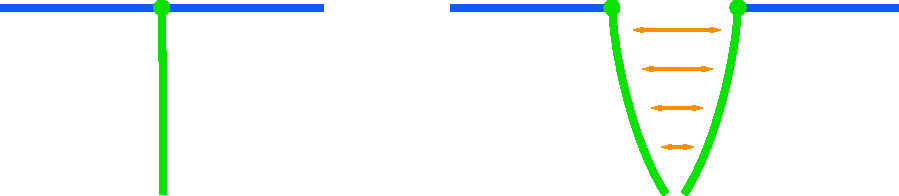
\includegraphics[scale = 0.7]{no_mfld}
\caption{Left: In the brane perspective, the bath CFT on the asymptotic boundary (blue) is connected to two copies of the effective CFT on the brane (green) but the resulting geometry is not a manifold. Right: For excitations below the effective CFT cutoff the system behaves as if it consists of two systems on a manifold which are weakly coupled in the gravitational region (green).}
\label{fig:no_mfld}
\end{figure}

First, we note that constructions where multiple CFTs are joined at a common defect are not rare. For example they appear in the study of boundary and interface CFTs (\eg see \cite{Chiodaroli:2012vc}), and sometimes seem to be required to remove anomalies \cite{Ooguri:2020sua}.

Second, we would like to argue that in the regime where the defect theory can be described by two copies of the boundary CFT coupled to Einstein gravity, we can approximately think of the full theory as two copies of the orbifolded theory (each living on a manifold), which are weakly coupled in the gravitational region -- see the right panel of figure \ref{fig:no_mfld}. This is particularly easy to see from the bulk perspective. For brevity we restrict ourselves to the discussion of graviton modes, but a similar story applies to all bulk fields. 

Let us begin by recalling that for $\veps \ll 1$, the spectrum of graviton fluctuations in the bulk is almost unchanged with respect to the modes in (two copies of) empty AdS space. Hence much of the corresponding physics should be very similar that of two copies of the the AdS$_{d+1}$, or to two copies of the dual CFT$_d$ on the boundaries of two independent AdS$_{d+1}$ geometries. Of course, one exception to the preceding is that upon gluing the two AdS$_{d+1}$ geometries together, a new set of very light graviton states localized in the vicinity of the brane \cite{Randall:1999vf,Randall:1999ee,Karch:2000ct,Karch:2001jb}, as discussed in section \ref{face}. For simplicity, we refer to the latter as the brane graviton modes, while we refer to the former as the standard normalizable modes.\footnote{These bulk modes are $\mathbb Z_2$ graded under reflection across the Planck brane, and the even modes survive the $\mathbb Z_2$ orbifold discussed above include the brane graviton states as well as half of the standard normalizable modes. However, this organization of the modes is not useful for the following discussion.}

On a fixed time slice, as shown in the right panel of figure \ref{fig:brane2}, the standard normalizable modes will describe stress energy excitations in the dual CFT on both the left and right halves of the asymptotic boundary. If we assume an approximate extrapolate dictionary \cite{Harlow:2011ke} for the brane theory as well, these normalizable modes will also describe analogous excitations for the effective CFT on the brane. However, there will be two sets of such excitations: those described by bulk excitations\footnote{We stress here that the localized excitations considered here do not correspond to individual energy eigenmodes, which were implicit in the previous paragraph. Rather they will consist of linear combinations of such eigenmodes evaluated on the fixed time slice being examined here. Of course, having superpositions of energy eigenmodes is what produces the complicated time evolution described below.} with support primarily in the right copy of the AdS$_{d+1}$ geometry, and those described by the analogous excitations primarily in the left AdS$_{d+1}$ geometry. Hence, the stress tensor on the brane can be decomposed into two pieces which correspond to subsectors of the brane theory, each of which is determined by bulk excitations which essentially live on one side of the brane. If these subsectors were truly superselection sectors (\eg as one might imagine arises in the limit $\veps\to0$), our brane theory would contain two independent copies of the boundary CFT  and each of these copies would only interact with the bath CFT on the corresponding half of the asymptotic boundary. That is, each of these systems would live on an independent manifold with topology $S^{d-1} \times \mathbb R$. 

However, this is not strictly correct and the two copies of the CFT on the brane are weakly coupled with $\veps\ll1$ but finite. In particular, localized stress energy excitations of the form considered above will not remain localized with time evolution. Rather they will eventually spread across the entire asymptotic boundary if time evolves for a sufficiently long time. For example, an excitation localized on the right asymptotic boundary will evolve to eventually produce excitations of the stress tensors on the left asymptotic boundary and on the brane as well. From the boundary perspective, excitations moving onto the brane correspond to excitations that are absorbed by the conformal defect (and remain there for a long time).

The spreading of the localized excitations can be seen to arise through two physical effects: First, the bulk excitations can tunnel between the two AdS$_{d+1}$ regions shown in figure \ref{fig:brane2}. Recall that (the radial part of) the linearized bulk equation of motion can be reduced to a Schroedinger equation with a double-well potential, where the height of the barrier is determined by the brane tension \cite{Karch:2000ct}. With $\veps\ll1$ but finite, the barrier height while large remains finite and there will be a finite probability for a bulk excitation on one side of the Planck brane to tunnel to the other. A second independent coupling comes because the stress tensors of the two copies of the CFT couple to the same gravity theory on the brane. From the bulk perspective, the nonlinear Einstein equation produces interactions between the brane graviton modes with excitations on either side of the brane. Hence bulk excitation excitations on one side can leak to the other side by scattering process involving the brane gravitons. However, we note that both effects become smaller as the brane tension approaches its critical value, \ie as $\veps$ approaches zero. Thus, to a good approximation, the brane theory can be treated at two copies of the boundary CFT which only interact weakly. \\


\hd{Entanglement wedge cross-sections:} Recent work \cite{Takayanagi:2017knl,Nguyen:2017yqw} has drawn attention to
the entanglement wedge cross-section, \ie for disconnected boundary regions, the codimension-two surfaces in the bulk which have minimal area and which split the entanglement wedge in two. In particular, there are a number of proposals relating these holographic surfaces to various entanglement measures: entanglement of purification \cite{Takayanagi:2017knl,Nguyen:2017yqw}, reflected entropy \cite{Dutta:2019gen},  odd entanglement entropy \cite{Tamaoka:2018ned,Kusuki:2019evw,Kusuki:2019rbk}, or entanglement negativity \cite{Kudler-Flam:2018qjo,Kusuki:2019zsp}. 

Turning to our model and examining figure \ref{fig:RTPhases}, we see that there are two such minimal surfaces in the connected phase, for which a quantum extremal island appears on the brane. These surfaces are simply disks of radius $P=P_0$ on either side of the brane, with area
\beq\label{reflw}
A=\frac{2\,L^{d-1}\, \Omega_{d-2}}{d-1} \ P_0^{d-1}\, {}_{2}F_1\left[ \frac{1}{2},\frac{d-1}{2},\frac{d+1}{2},-P_0^2 \right]\,,
\eeq
as can be seen from eq.~\reef{A_disc}. The fact that both disks have the same area results from the fact that the corresponding boundary regions are symmetric on either of the conformal defect -- see figure \ref{EEprob}. Of course, if one of the two caps comprising the boundary regions was smaller, the minimal area disk closer to this cap would provide the global minimum and hence become the entanglement wedge cross-section. It would be interesting to understand if the second minimal disk also plays an interesting role in characterizing the entanglement of the boundary state. In this vein, let us add that there are also two additional extremal disks which divide the entanglement wedge in two but their area is actually a local maximum. These disks again lie on either side of the brane but end on $\sigma_\xR$, the intersection of the RT surface with the brane. Again, it is natural to wonder if these surfaces have an interpretation in terms of the boundary entanglement. Let us note that similar surfaces appear in the following discussion.\\

\hd{RT Bubbles and Wormholes:} 

	In appendix \ref{bubble}, we consider a surprising class of RT surfaces with the topology of a sphere, \ie $S^{d-1}$ in the ($d+1$)-dimensional bulk. The appearance of these extremal `bubbles' is quite unusual as they are homologous to the entire boundary. Hence the standard RT prescription would assign an entropy to the ground state of the dual boundary system. Further, presence of a `zero mode' which allows the bubbles to be translated along the brane makes their interpretation even more puzzling. An essential feature for the appearance of the RT bubbles was that the gravitational coupling in the DGP term \reef{newbran} was negative, \ie $\lamb<0$. We also noted that the bubbles do not appear to be macroscopic objects in the brane theory. Rather, as shown in eq.~\reef{haiku2}, their size is always of order of the effective cutoff $\tilde\delta$.
	
Despite the unusual features of these RT bubbles, the discussion in appendix \ref{bubble} highlights a general feature of the quantum extremal islands in a simple way. In particular, as discussed below eq.~\reef{genbubble1}, there are two competing terms contributing to the generalized entropy of these surfaces: the bulk area which describes the entropy of the CFT fields on the brane enclosed by the bubble and the area of the boundary where they intersect the brane, which appears in the gravitational entropy of the DGP term. The bulk contribution naturally acts to contract the bubble but with $\lamb<0$, the brane contribution acts to expand the bubble. As described in the appendix, there is an equilibrium radius where these two effects balance one another. Of course, with $\lamb>0$, the brane contribution also acts to contract the boundary of the bubble and so no closed extremal surfaces appear, as expected.

As noted above, a similar competition is a general feature in the formation of quantum extremal islands. However, in this case as discussed in section \ref{sec:enzyme}, the bulk and brane contributions combine to produce a Bekenstein-Hawking term $\area(\sigma_\xR)/{4G_\mt{eff}}$ on the boundary of the island. This contribution, of course, imposes a large penalty to the formation of a large island and acts to contract the boundary towards a smaller (\ie vanishing) radius. For an island to appear, this contraction must be balanced by an expanding contribution. From the bulk perspective, this is simply coming from the remaining\footnote{We combined part of the bulk area into the Bekenstein-Hawking term above.} bulk area contribution of the RT surface, which we can ascribe to the quantum EE of the CFT state from the brane perspective. The point to be noted here is that for this to provide an expansion the RT surface must be anchored far from the island, \ie in the asymptotic (nongravitational) region associated with the boundary CFT. While perhaps self-evident, this discussion highlights the nonlocal nature of the physics producing the quantum extremal islands.

Let us add that the quantum extremal islands discussed here (as well as the RT bubbles) are remnants of replica wormholes in the limit $n\to1$. This follows from the fact that we are simply studying holographic EE with RT surfaces in a new bulk background, \ie with a back-reacted brane. Hence the analysis of \cite{Lewkowycz:2013nqa}\footnote{Following \cite{Dong:2016hjy,Faulkner:2017vdd}, the same applies for general time dependent situations.} introduces a smooth $n$-fold covering geometry for the corresponding Renyi entropies with positive integer indices. These covering geometries produce smooth wormhole geometries on brane analogous to those discussed in \cite{Almheiri:2019qdq,Penington:2019kki} for two dimensions. 

Now assuming replica symmetry, one can then take a $\mathbb Z_n$ orbifold quotient which leaves a single copy of the boundary geometry but the bulk solution now contains a codimension-two cosmic brane with tension $T_n=(n-1)/(4\Gbk\,n)$. In the presence of a DGP brane, we expect that there is an additional contribution where the two branes intersect, \ie the intersection surface carries an intrinsic tension $\widehat T_n=(n-1)/(4\Gbr\,n)$. In this setting, our discussion above for the formation of quantum extremal islands extends to the Renyi entropies in a relatively straightforward way. In particular, we expect that an area contribution associated with the boundary of the island now carries an effective tension $\tilde T_n=(n-1)/(4G_\mt{eff}\,n)$, which combines the intrinsic tension of this intersection surface and the contribution of the cosmic brane in the vicinity of the Planck brane. The contraction created by this term must be balance by the expansion provided by the remaining cosmic brane contributions. However, to provide an expansion the cosmic brane must be anchored by a twist operator in the asymptotic (nongravitational) boundary. Again, this highlights the nonlocal nature of the physics which implicitly supports the replica wormholes.

Of course, these dynamical considerations are emergent in the topological models considered in \cite{Marolf:2020xie,Penington:2019kki}. Hence it would be interesting to understand the implications of this dynamics to extend the new discussions of baby universes and ensembles to higher dimensions.\\



To conclude, let us comment that we will build on the holographic model constructed here to study the Page curve and the appearance of quantum extremal islands for higher dimensional black holes in \cite{QEI}. In particular, we study eternal black holes coming to equilibrium with an external heat bath (prepared at the same temperature) in a higher dimensional analog of the analysis appearing in \cite{Almheiri:2019yqk}. Let us reiterate that unconventional features (\ie Gauss-Bonnet and DGP couplings) introduced to favour quantum extremal islands here are unimportant in the discussion of higher dimensional black holes.\\





%%% Local Variables:
%%% mode: latex
%%% TeX-master: "../lifeonbrane3"
%%% End:




\section*{Acknowledgments}
We would like to thank Ahmed Almheiri, Raphael Bousso, Xi Dong, Netta Engelhardt,  Zach Fisher, Greg Gabadadze, Juan Hernandez, Don Marolf, Shan-Ming Ruan, Edgar Shaghoulian, Antony Speranza and Raman Sundrum for useful comments and discussions. Research at Perimeter Institute is supported in part by the Government of Canada through the Department of Innovation, Science and Economic Development Canada and by the Province of Ontario through the Ministry of Colleges and Universities. RCM is supported in part by a Discovery Grant from the Natural Sciences and Engineering Research Council of Canada, and by the BMO Financial Group. HZC is supported by the Province of Ontario and the University of Waterloo through an Ontario Graduate Scholarship. RCM and DN also received funding from the Simons Foundation through the ``It from Qubit'' collaboration. The work of IR is funded by the Gravity, Quantum Fields and Information group at AEI, which is generously supported by the Alexander von Humboldt Foundation and the Federal Ministry for Education and Research  through the Sofja Kovalevskaja Award. IR also acknowledges the support of the Perimeter Visiting Graduate Fellows program and the hospitality of Perimeter Institute, where part of this work was done. JS acknowledges the support of the Natural Sciences and Engineering Research Council of Canada (NSERC).

\appendix

\section{Generalized Entropy on the Brane}\label{generalE}
% !TEX root = ../lifeonbrane3.tex
%

In sections \ref{sec:two-d} and \ref{sec:DGP}, we introduced intrinsic gravitational terms to the brane action. Following \cite{Almheiri:2019hni},\footnote{See also \cite{Almheiri:2019psf, Almheiri:2019yqk, Chen:2019uhq, Penington:2019kki, Almheiri:2019qdq}.} we assumed that these terms contribute to the generalized entropy, \eg see eq.~\reef{eq:sad0} or \reef{eq:sad}.
In this appendix, we present a extended version of an argument in \cite{Myers:2010tj}, which will support this assumption and our formula for generalized entropy. 

As in the main text, we begin with a $d$-dimensional holographic CFT on $R\times S^{d-1}$ with a conformal defect on the equator of the sphere, sweeping out $R\times S^{d-2}$. On a fixed time-slice, we choose an entangling surface $\SCFT$ which divides the sphere into two equal halves along a maximal $S^{d-2}$ which lies orthogonal to the conformal defect. Now we wish to determine the entanglement entropy between the two halves
of the system, as sketched in figure \ref{fig:defect}. Recall that with the geometric approach \cite{Callan:1994py}, we must evaluate the partition function on a (Euclidean) background geometry with an infinitesimal conical defect. In order to construct a symmetric geometry where introducing such a defect is well-defined, we perform a Wick rotation on the boundary time (\ie $t_\mt{E}=it$) and then conformally transform the Euclidean background metric to a round $S^{d}$ with the conformal defect lying on a maximal $S^{d-1}$ on this background. Now $\SCFT$ remains a maximal $S^{d-2}$ which runs orthogonal to the defect and pierces the latter on a $S^{d-3}$. With this construction, there is a rotational symmetry in the two dimensions orthogonal to $\SCFT$. To evaluate the corresponding entanglement entropy, we construct $\mathcal{M}_{1-\eps}$, the `$n$-fold cover' with $n=1-\eps$, by introducing an infinitesimal conical defect at $\SCFT$. The entanglement entropy is then given by
\beq\label{entro9}
S = \lim_{\eps\to0}\left( \frac{\partial\ }{\partial\eps}+1 \right)\log
Z_{1-\eps}\,,
\eeq
where $Z_{1-\eps}$ is the partition function of the holographic CFT on the covering space $\mathcal{M}_{1-\eps}$. Of course, the latter has a dual description in terms of the bulk gravity, and using the usual saddle point approximation, eq.~\reef{entro9} becomes \cite{Myers:2010tj}
\beq\label{entropylimit}
S =-\lim_{\epsilon\to0}\Big(\frac{\partial}{\partial \epsilon} + 1\Big) I_{E, 1-\epsilon}\,,
\eeq 
where $I_{E,1-\epsilon}$ is the Euclidean bulk action evaluated on the appropriate dual solution.
%
%\begin{figure}[h]
%	\def\svgwidth{0.3\linewidth}
%	\centering{
%		\input{defect.pdf_tex}
%		\caption{A timeslice of our $d$-dimensional CFT setup with entangling surface $\Sigma_\mt{CFT}$. An infinitesimal conical defect $\Sigma_\xR$ runs through the bulk and intersects the brane at $\sigma_\xR$.} \label{fig:defect}
%	}
%\end{figure}
\begin{figure}[h]
	\def\svgwidth{0.6\linewidth}
	\centering{
		\input{defect31.pdf_tex}
		\caption{A timeslice of our $d$-dimensional CFT setup with entangling surface $\Sigma_\mt{CFT}$ and an equatorial conformal defect (the green line). In the right panel, one dimension is suppressed relative to the left panel.} \label{fig:defect}}
\end{figure}

Setting $n=1$ for a moment, the bulk dual of $\mathcal{M}_{1}$ is simply the Euclidean version of the geometry constructed in section \ref{BranGeo}, which we denote $\widetilde{\mathcal{M}}_{1}$. Recall the boundary geometry is $S^{d}$ and the conformal defect runs around a maximal $S^{d-1}$. In the bulk, the geometry is locally EAdS$_{d+1}$ everywhere away from the brane, and the brane has a EAdS$_d$ geometry which extends out to the conformal defect at the asymptotic boundary and with the curvature scale given by eq.~\reef{curve1} -- see figure \ref{fig:defect2}. Now the  entangling surface $\SCFT$ on the asymptotic AdS boundary is the boundary of an extremal surface $\Sigma_\xR$ in the bulk, which runs  straight across the bulk solution and has a EAdS$_{d-1}$ geometry with curvature scale $L$.  This surface pierces the brane at a right angle and the intersection, another extremal surface $\sigma_\xR$, has the geometry of a EAdS$_{d-2}$ with curvature scale $\ell_\mt{B}$ -- see figure \ref{fig:defect2}. Now because of the symmetry of this configuration, the rotational symmetry about the entangling surface in the boundary extends to a rotational symmetry about $\Sigma_\xR$ in the bulk. Hence we can calculate the entanglement entropy with the same geometric approach as we applied in the boundary. That is, we construct $\widetilde{\mathcal{M}}_{1-\eps}$, the $n$-fold cover (with $n=1-\eps$) of the bulk solution  with a infinitesimal conical defect at $\Sigma_\xR$ and by extension, at $\sigma_\xR$ on the brane. 

\begin{figure}[h]
	\def\svgwidth{0.6\linewidth}
	\centering{
		\input{defect32.pdf_tex}
		\caption{A cross-section of the Euclidean geometry $\widetilde{\mathcal{M}}_{1}$. The orange semicircle and its complement along a time slice represent the orange shaded region of figure \ref{fig:defect} and its complement. The rotation that keeps $\Sigma_\mt{CFT}$ fixed represents euclidean time. An infinitesimal conical defect $\Sigma_\xR$ runs through the bulk and intersects the brane at $\sigma_\xR$.} \label{fig:defect2}
	}
\end{figure}

That is, the angle around $\Sigma_\xR$ runs through a range $2\pi(1-\epsilon)$. Now  \cite{Fursaev:1994ea,Fursaev:1995ef} developed a description of such conical defects in which the singular geometry is replaced by a `regulator' geometry where the region
around the conical singularity is smoothed out. Applying their key result, we can write the bulk Riemann tensor  as a ``smooth" contribution away from $\Sigma_\xR$, the conical defect, and a singular order $\epsilon$ contribution at $\Sigma_\xR$,\footnote{This order $\eps$ contribution is universal, whereas the details of the regulator come into play at order $\eps^2$ and higher.}
\beq\label{separation}
^{(\epsilon)}R^{ab}{}_{cd} = R^{ab}{}_{cd}+2\pi \epsilon\, {\varepsilon}^{ab}{\varepsilon}_{cd}\,\delta_{\Sigma_\xR}\,,
\eeq 
where ${\varepsilon}_{ab}$ is the Euclidean volume form in the two-dimensional transverse space to $\Sigma_\xR$, and $R^{ab}{}_{cd}$ is the ``smooth" curvature piece. The $\delta_{\Sigma_\xR}$ is a two-dimensional delta function defined in \cite{Myers:2010tj}. The conical singularity intersects the brane at $\sigma_\xR$ and so we have a similar decomposition for the Riemann tensor on the brane,
\beq\label{separation2}
^{(\epsilon)}\tilde R^{ij}{}_{k\ell} = \tilde R^{ij}{}_{k\ell}+2\pi \epsilon \,\tilde{\varepsilon}^{ij}\tilde{\varepsilon}_{k\ell}\,\delta_{\sigma_\xR}\,.
\eeq 

Now recall that our aim is to evaluate the Euclidean action in eq.~\reef{entropylimit}. This action is the sum of the Euclidean versions\footnote{Note that the difference in signs in going between Minkowski and Euclidean signatures \cite{Myers:2010tj}.} of the bulk and brane actions in eqs.~\reef{act2} and \reef{newbran} (or perhaps eq.~\reef{JTee} for $d=2$), as well as the associated boundary terms. Equipped with eqs.~\reef{separation} and \reef{separation2}, it can be shown that in the limit of small $\epsilon$ that the Euclidean action can be expanded as
\beqa\label{epsilonaction}
I_{E,1-\epsilon}& =& (1-\epsilon)I_{E,1} +
 \int_\mt{bulk}\!\! d^{d+1}x \sqrt{g}\, 2\pi \epsilon {\varepsilon}^{ab}{\varepsilon}_{cd}\,\delta_{\Sigma_\xR}\, \frac{\partial \mathcal{L}_\mt{E,bulk}}{\partial R^{ab}{}_{cd}}\\
 %
&&\qquad+\int_\mt{brane}\!\!\!\! d^{d}x \sqrt{\tilde g} \, 2\pi \epsilon \tilde{\varepsilon}^{ij}\tilde{\varepsilon}_{k\ell}\,\delta_{\sigma_\xR}\,  \frac{\partial \mathcal{L}_\mt{E,brane}}{\partial \tilde{R}^{ij}{}_{k\ell}} +\mathcal{O}(\epsilon^2)\,.
\eeqa
Noting the symmetry of our configuration, \ie the curvatures are constant everywhere along the surfaces $\Sigma_\xR$ and $\sigma_\xR$,
we then find the entropy in eq.~(\ref{entropylimit}) is given by
\beq\label{fish9}
S = -2\pi \frac{\partial \mathcal{L}_\mt{E,bulk}}{\partial R^{ab}{}_{cd}} {\varepsilon}^{ab}{\varepsilon}_{cd} \int_{\Sigma_\xR} d^{d-1}x \sqrt{h}-2\pi \frac{\partial \mathcal{L}_\mt{E,brane}}{\partial \tilde{R}^{ij}{}_{k\ell}} \tilde{\varepsilon}^{ij}\tilde{\varepsilon}_{k\ell} \int_{\sigma_\xR} d^{d-2}x \sqrt{h'}\,,
\eeq 
where $h$ and $h'$ are the induced metrics along the $\Sigma_\xR$ and $\sigma_\xR$, respectively. Hence we see that there is a contribution of the Wald entropy from both the bulk action and the brane action. Further, let us note that various signs appear upon analytically continuing back to Lorentzian spacetime, \ie in the Lagrangian and the transverse volume form \cite{Myers:2010tj}. 


For the case where the Einstein-Hilbert action appears both in the bulk and on the brane, as in eqs.~\reef{act2} and \reef{newbran}, we find the formula for the generalized entropy \reef{fish9} becomes
\beq\label{fish88}
S = \frac{A(\Sigma_\xR)}{4 G_\mt{bulk}}+ \frac{A(\sigma_\xR)}{4 G_\mt{brane}}\,,
\eeq
as given in equation \reef{eq:sad}. The present derivation only applies to special symmetric configuration, as in \cite{Myers:2010tj}. The symmetry of this configuration preculdes finding any extrinsic curvature terms in eq.~\reef{fish9}, as would be expected for the Dong entropy \cite{Dong:2013qoa}. We note however that no such terms would correct eq.~\reef{fish88} for the generalized entropy coming from the Einstein-Hilbert term. It would, of course, be interesting to extend our derivation to more general configurations involving bulk DGP branes, along the lines of \cite{Lewkowycz:2013nqa} or \cite{Dong:2016hjy}.

%As a final note here, let us observe that our derivation of eq.~\reef{fish88} involved explicitly introducing a  comparing this singular approach to \cite{Lewkowycz:2013nqa} as Callan-Wilczek \cite{Callan:1994py} is to Gibbons-Hawking \rcm{ref??}


\section{RT Bubbles}
\label{bubble}
% !TEX root = ../lifeonbrane3.tex
%





%\subsection{`Bubbles' on the brane}\label{bubblesX}


In this appendix, we consider a simple but surprising class of RT surfaces. In particular, we show below that there are closed extremal surfaces with the topology of a sphere, \ie $S^{d-1}$ in the locally AdS$_{d+1}$ bulk geometry. In empty AdS space, one could consider such spherical surfaces, but their area would be extremized when they collapse to zero size. In the present case, we will show that in certain situations, the spherical RT surfaces can be supported at finite size by the brane.  To illustrate the situation, we continue with the special case of $d=3$ as in section \ref{sec:examples}, and afterwards comment on the situation with general $d$. 
%
%\begin{figure}[h]
%\begin{center}
%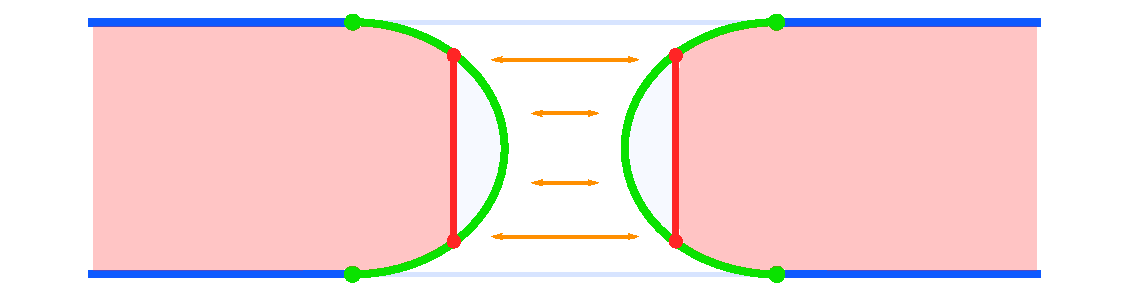
\includegraphics[scale=0.2]{images/bubble}
%\caption{One half of an RT bubble supported on the brane. \rcm{Lets illustrate this in the `style' of figure \ref{fig:EWs}.}}
%\label{figbubble}
%\end{center}
%\end{figure}

\begin{figure}[h]
	\def\svgwidth{0.8\linewidth}
	\centering{
		\input{bubble.pdf_tex}
		\caption{An RT `bubble' on the brane: even for the vacuum, when $\Gbr<0$ the competing bulk and brane area terms can lead to a stable extremal surface, which is  homologous to the entire time slice for the boundary CFT. The entanglement wedge then corresponds to the shaded red region. Since the two sides of the brane are glued together, the RT surface has the topology of $S^{d-1}$. }
		\label{figbubble}
	}
\end{figure}

Consider the geometry illustrated in figure \ref{figbubble}. On either side of the brane, we have a disk satisfying $\zeta=$constant, \ie satisfying eq.~\reef{zetap} with $P_0=0$. Hence locally these surfaces extremize the entropy functional \reef{area} in the bulk. However, rather than extending out to the asymptotic boundary, as shown in the figure, the two disks intersect the brane and meet at some radius $\pb$.  Hence this RT surface has the topology of a sphere and we use the nomenclature `bubble' to describe these surfaces. For $d=3$, the generalised entropy \reef{eq:sad} of this bubble is
\begin{align}\label{Agenbubble}
\sgen&=\frac{\pi L^2}{\Gbk} \left(  \sqrt{1+\pb^2}-1  + \lamb\, \pb \right) +2\,\lgb 
\end{align}
with $\lamb$ defined in eq.~\eqref{newdefs}. We have also included the topological term introduced in eq.~\reef{Euler3}.
Of course, since these surfaces never reach the asymptotic boundary, this quantity is finite, \ie there are no UV divergences in eq.~\reef{Agenbubble}. 

Extremizing eq.~\reef{Agenbubble} with respect to the radius of the bubble, we find
\beq\label{gamdot}
\partial_{\pb}\sgen=0 \qquad
\implies\qquad \frac{\pb}{\sqrt{1+\pb^2}}=-\lamb=-\frac{\Gbk}{2L\,\Gbr}\,.
\eeq
Now recall that we will always have $\Gbk>0$, but considered the possibility of $\Gbr$ becoming negative in section \ref{sec:examples}. Let us first consider the case $\lamb\ge 0$, which implies $1/\Gbr\ge 0$. In this case, we can not satisfy eq.~\reef{gamdot}, since both the bulk and brane contributions to the generalised entropy \eqref{Agenbubble} are positive and monotonically increasing functions of $\pb$. Therefore the minimum lies at $\pb=0$, \ie where the bubble collapses to zero size -- see figure \reef{figAbubble}. 

Of course, the more interesting scenario is when $\lamb$, and hence
$1/\Gbr$, are negative. Then eq.~\reef{gamdot} has the solution
\begin{align}
\pbo=-\frac{\lamb}{\sqrt{1-\lamb^2}}\,,
\label{cookie}
\end{align}
for which the generalized entropy \reef{Agenbubble} becomes
\begin{align}\label{Sbubble}
\sgen= \frac{\pi L^2}{\Gbk} \left( \sqrt{1-\lamb^2} - 1 \right)+2\,\lgb .
\end{align}
We note that these expressions are only sensible for $-1<\lamb<0$. In fact, for $\lamb<-1$, there is no minimum for the generalized entropy \reef{Agenbubble}, \ie there is no solution for eq.~\reef{gamdot}, and rather $\pb$ runs off to infinity -- see figure \reef{figAbubble}.  This is, perhaps, not so surprising since we can see from eq.~\reef{Newton34} that this regime is pathological, with the graviton localized on the brane becoming a ghost.

Therefore we only consider the regime $-1<\lamb<0$ where eqs.~\reef{cookie} and \reef{Sbubble} apply. As illustrated in figure \reef{figAbubble}, eq.~\reef{cookie} is indeed the global minimum of the generalized entropy \eqref{Agenbubble}. We might note that the sum of the bulk and brane terms in eq.~\reef{Sbubble} is negative. That is, the combined contributions of the two area terms in eq.~\reef{eq:sad} is in fact {\it negative!} Hence we only get a sensible (\ie positive) result for the generalized entropy \reef{Agenbubble} with the inclusion of the topological term \reef{Euler3} and with $\lgb$ sufficiently positive, which was also favoured in section \ref{sec:examples}.
%
%\begin{figure}[h]
%\begin{center}
%\includegraphics[scale=0.4]{images/Abubble}
%\caption{The generalised area \eqref{Agenbubble} for a bubble as a function of its radius. For $\lamb>0$, the area is minimal for vanishing size, whereas for $-1<\lamb<0$ it has a finite size. For $\lamb<-1$, there is no global minimum, signalling an instability of the system. }
%\label{figAbubble}
%\end{center}
%\end{figure}

\begin{figure}[h]
	\def\svgwidth{0.8\linewidth}
	\centering{
		\input{bubblePlot.pdf_tex}
		\caption{The generalised area \eqref{Agenbubble} for a bubble as a function of its radius. For $\lamb>0$, the area is minimal for vanishing size, whereas for $-1<\lamb<0$ it has a finite size. For $\lamb<-1$, there is no global minimum, signalling an instability of the system. Further note that as $P_0$ approaches zero, $S_\mt{gen}\to \pi L^2/ G_\mt{bulk}$ since we have set $\lgb=\pi L^2/(2G_\mt{bulk})$.
		}
		\label{figAbubble}
	}
\end{figure}


These calculations are easily extended to higher dimensions, where eq.~\reef{Agenbubble} is replaced by
\beq\label{genbubble1}
S_\mt{gen}=\frac{L^{d-1}\,\Omega_{d-2}  }{2(d-1)\Gbk}\,\pb^{d-1}\ {}_{2}F_1\!\left[ \frac{1}{2},\frac{d-1}{2},\frac{d+1}{2},-\pb^2 \right]+\frac{L^{d-2}\, \Omega_{d-2}}{4\Gbr}\,\pb^{d-2}\,.
\eeq
We have not included contributions from any topological gravity terms in this expression for general $d$ -- see further comments below. To produce a qualitative understanding of this expression, 
we note that
\beq
  \hyperF\!\left[\frac{1}{2}, \frac{d-1}{2}, \frac{d+1}{2}, -\pb^2 \right]  \simeq\begin{cases}
  1 & \text{if $\pb\ll 1$}\,,
  \\
  \frac{d-1}{d-2}\frac{1}{\pb} &\text{if $\pb\gg 1$}\,.
\end{cases}
\label{eq:bubblegum}
\eeq
Now, we observe that for large $\pb$, the leading contribution in eq.~\reef{genbubble1} takes the expected form
\beq\label{expect4}
\sgen\simeq \frac{A(\sigma_\xR)}{4G_\mt{eff}} +\cdots \qquad{\rm where}\ \ \ \frac{A(\sigma_\xR)}{4G_\mt{eff}}=\frac{L^{d-1}\,\Omega_{d-2}  }{2(d-2)\Gbk}\,(1+\lamb)\,\pb^{d-2}\,,
\eeq
again using eq.~\eqref{newdefs}. Hence, there is a large penalty for having the RT surface meet the brane at a large radius $\pb$, which  will tend to push the intersection $\sigma_\xR$ to smaller radii. However, for small $\pb$, the bulk contribution to $\sgen$  grows like the volume, \ie it is proportional to $\pb^{d-1}$. Hence in this regime, the brane contribution dominates since it is proportional to $\lamb\pb^{d-2}$, and for $\lamb<0$, this term will favour  larger values of $\pb$. Hence for the interesting case of $\lamb<0$, we can expect that the generalized entropy for general $d$ is extremized at some finite value of $\pb$ of order $-\lamb$, just as we found for $d=3$. Of course, the denominator in eq.~\eqref{cookie} is also important for $\lambda_b$ close to $-1$, but this can not be seen with this simple qualitative analysis. Now, in fact, the extremality condition can in fact be solved exactly for any $d$. One finds
\beq\label{amazing}
  \partial_{\pb} S_\gen
  = \frac{L^{d-1}\,\Omega_{d-2}}{2 G_\bulk}\, \pb^{d-3}\left(
  \frac{\pb}{\sqrt{\pb^2+1}} + \lamb \right)=0\,.
\eeq
Of course, for $\lamb\ge0$, the only solution is $\pb=0$, \ie the bubble collapses to zero size, as expected. However, for $\lamb<0$, the minimum is given by $\pb=\pbo$, precisely the same critical  radius as in eq.~\eqref{cookie}. Substituting this critical radius into the generalized entropy \reef{genbubble1} does not yield any simplifications, however the result is easily evaluated numerically as a function of $\lamb$. Of course, the generalized entropy \reef{genbubble1} is negative at this minimum and so one would really need to add a topological term to the gravitational theory, either in the bulk or on the brane, to produce a sensible entropy, as we did for the $d=3$ example.


\subsection*{Wormholes and Cutoffs} %\label{wormy}

The appearance of these extremal bubbles is quite unusual, of course. Since they are homologous to the entire boundary, this suggests that the ground state of the dual boundary system has an entropy by the standard RT prescription. The bulk construction makes clear that it is the conformal defect which introduces this large degeneracy of ground states.\footnote{As we see in figure \ref{figAbubble}, entropy associated with the zero-size bubble is nonvanishing and higher than that of the stable finite-size bubble due to the topological contribution. However, we note that it may be that the correct RT prescription is to choose `empty surface' in this case, giving zero entropy.} %\vc{Are we really getting a mixed state of degenerate ground states? What would purify this? (I'm having a hard time picturing a path integral construction of this state. Especially in the boundary picture, it's hard to see how the path integral can create a mixed state.) Also, I'm confused about the sign of the bubble entropy. It seems we have two possibilities: we include $\lambda_{GB}$ (maybe we don't actually need to) so that the positive topological contribution plus the otherwise negative entropy of a single fixed bubble plus the positive(?) volume degeneracy (described below) is positive; or all that stuff sums to a negative value. In the first case, wouldn't the RT prescription tell us to choose the empty surface, giving a zero entropy? In the second case, how can we interpret a negative entropy as a ground state degeneracy?}

We should note, however, that the evaluation of this ground state entropy presented above is incomplete. In particular, there is a `zero mode' associated with these bubbles which allows them to be translated along the brane. Recall that while the empty AdS$_{d+1}$ geometry has an $SO(2,d)$ isometry (reflecting the conformal symmetry group of the boundary CFT), the backreacted brane geometry preserves an $SO(2,d-1)$ subgroup of these symmetries. Now our construction places the center of the bubbles at $P=0$, however, by acting with these symmetries, we can position the center anywhere on the brane. Further recall that one arrives at the RT prescription by evaluating (a particular limit of) a saddlepoint in the gravitational path integral \cite{Lewkowycz:2013nqa}. Hence we have discovered that there is a zero mode associated with the saddlepoints connected to the bubbles. Hence the integral over this zero mode would add a contribution to the entropy proportional to the logarithm of the (regulated) brane volume. It is interesting to speculate that this contribution may lift the negative value for $S_\mt{gen}(\pbo)$ to some positive entropy.

An essential feature required for the appearance of these bubbles was that the gravitational coupling associated with the DGP term \reef{newbran} was negative, \ie $1/G_\brane<0$. While this may seem unusual, let us note that integrating out quantum fields on the brane can produce either a positive or negative shift in Newton's constant. In particular, the shift is found to be negative for a $U(1)$ gauge field when $d<8$ \cite{Larsen:1995ax,Kabat:1995eq}. With the connection between the renormalization of Newton's constant and the area law contribution in entanglement entropy \cite{Callan:1994py,Susskind:1994sm}, this negative renormalization generates a puzzle which, however,  was finally resolved in terms of edge modes in \cite{Donnelly:2014fua,Donnelly:2015hxa}. There is a similar negative renormaliation for non-minimally coupled scalars \cite{Larsen:1995ax}, for which the resolution of the associated puzzle appears  in \cite{Faulkner:2013ana}. However, we should add that if we imagine $1/G_\brane<0$ is induced by additional quantum fields on the brane, then our entanglement entropy calculations are incomplete as they do not fully include the contributions of these extra fields. Hence our perspective here is to simply view the DGP term as a counterterm as would appear in the usual quantization of gravity on the brane, and in this context, the sign of $1/G_\brane$ is not proscribed but rather is chosen as needed to produce the `observed' value of $1/G_\mt{eff}$.

Another remark in this vein is that the bubble solutions appear as soon as $1/G_\brane$ is negative, \ie these solutions \reef{cookie} exist for very small values of $\lamb$ as long as $\lamb<0$. However, it is important to recall that the short distance cutoff is given by eq.~\reef{ctoffminus} in this regime. Hence combining  eqs.~\reef{cylindd} and \reef{cookie},  the areal size of the bubbles becomes
\beq
L\pbo=\frac{|\lamb|\,L}{\sqrt{1-\lamb^2}}\simeq \frac{|\lamb|}{\sqrt{1+|\lamb|}}\,\tilde\delta\,.
\label{haiku2}
\eeq 
where we have substituted eq.~\eqref{haiku} in the second expression.
This expression approaches the maximum size $\tilde\delta/\sqrt{2}$ as $\lamb\to-1$. That is, the radius of bubbles is always smaller than the cutoff scale $\tilde\delta$ on the brane! Therefore, these solutions are not reliable in the regime where Einstein gravity gives a good description of the brane.  On the other hand, our calculations in this appendix involved evaluating RT surfaces in the bulk, \ie they only depended on bulk perspective. Further, for $|\lamb|\gtrsim1/\sqrt{2}$, the corresponding RT surfaces grow much larger than the bulk AdS scale, and so would be seen as valid solutions. 
%\vc{How can we know that a negative $G_\brane$ we have chosen still permits a good semiclassical theory up to a certain scale in the bulk perspective? (E.g.~from the bulk perspective alone, we can't even see that a $\lambda_b<-1$ produces ghost-like modes. It seems we can only be sure we have a good theory after comparing the DGP and induced actions, i.e.~taking the brane perspective.)}
However, one may ask if there are physical constraints which will not allow us to realize theories with $\lamb$ which are that negative and so prevent us from considering scenarios where these bubbles have a macroscopic size. 

We close here with two final remarks: These bubbles are a remnant of replica wormholes in the limit $n\to1$ \cite{Penington:2019kki,Hartman:2020swn}. In the discussion section, we explore if there are any lessons that they may hold for the new discussions of baby universes and ensembles \cite{Marolf:2020xie}. Another comment is that the bubble surfaces produce an interesting
entanglement wedge, which extends to a band  covering a finite time interval on the boundary. Of course, this is reminiscent of the holographic construction of differential entropy \cite{Balasubramanian:2013rqa,Balasubramanian:2013lsa,Czech:2014wka,Myers:2014jia,Headrick:2014eia}, which can be used to evaluate the area of closed surfaces in the bulk. It would be interesting to examine these connections further.


%%% Local Variables:
%%% mode: latex
%%% TeX-master: "../lifeonbrane3"
%%% End:


%\section{Thinking about Ensembles?}
%\label{ensign}
%% !TEX root = ../lifeonbrane3.tex
%



\rcm{lots of new references to read}

In order to derive the island formula, the appearance of wormholes in the replica trick is a crucial ingredient.
In the two-dimensional models involving JT gravity studied so far \cite{Almheiri:2019qdq,Penington:2019kki}, the existence of wormholes follows from the fact that JT gravity is defined by ensemble averaging over an ensemble of Hamiltonians.\footnote{For example, JT gravity emerges as the low energy effective description of the SYK model \cite{}, or has a UV complete definition in terms of a matrix model \cite{Saad:2019lba}.} In fact, by assuming ensemble averaging, one can easily reproduce many features \cite{Marolf:2020xie} demonstrated in the 2d models. 

However, it is generally assumed that in higher dimensions gravity on asymptotically AdS spacetimes is dual to a single, unitary theory.\footnote{The best known example is the duality between $\mathcal N=4$ super Yang-Mills theory and supergravity (or more precisely Type IIB string theory) on AdS${}_5\times S^5$.} In fact, in the higher dimensional case one would expect replica wormholes to be absent in any local theory. This can be seen by considering a theory on a higher-dimensional spacetime which couples to gravity in a subregion $U_\text{grav}$, and lives on a fixed background in the complement $U_\text{bath}$. If we want to compute the density matrix of a region $A \subset U_\text{bath}$, we are instructed to integrate out all degrees of freedom in the gravitating region $U_\text{grav}$. If we take products of the reduced density matrix -- like we would do in the replica trick -- no integral over the gravitating region is left to be performed and no Euclidean wormholes appear. More generally, in two dimensions, replica Wormholes appear in calculations of the spectral form factor and yield to a non-factorizability of products of the partition function. However, for a CFT${}_d$ the partition function is a number and a product of many partition functions clearly must factorize.

This opens the question if and how islands and replica wormholes appear in the higher dimensional case. As we have seen, in our model, they are readily explained from the bulk perspective, but in order to go beyond the case of holographic matter, it is important to also understand how they arise in the brane picture. Here, we will explain a possible mechanism suggested by the model discussed in this paper, and its relation to ensemble averaging.

As discussed in this paper, the description of the brane theory as a local CFT with a cutoff coupled to gravity in some region of space is only an effective one. In fact, we see from the bulk picture that the degrees of freedom in $U_\text{bath}$ and $U_\text{grav}$ are not independent. A particularly clear sign is the fact that under certain conditions parts of the gravitating region $\mathcal I_A \subset U_\text{grav}$ lie in the entanglement wedge of bath subregions $A \subset U_\text{bath}$. This signalled the appearance of an island on the brane picture. In this case, as is clear from EW reconstruction, specifying the state in $A$ also specifies the state in the island $\mathcal I_A$. In the presence of a brane, new bulk modes appear, which can be identified with the now-dynamical metric and sources of other primary operators on the brane. Specifying the state in $\mathcal I_A$ thus in particular means to specify the states of the metric and all other sources. The description that takes into account the link between degrees of freedom in the bath and the gravitating region corresponds to the full quantum gravity description of the state of \cite{Almheiri:2019yqk}.

In an effective, local and semi-classical approximation this link between the bath and the gravitating region is ignored so that $A$ and its associated island $\mathcal I_A$ are treated as independent subregions. If we are interested in a reduced density matrix $\rho^\text{s.c.}_A$ of a $A$ in the semi-classical approximation, we can obtain it from a fully quantum gravity density matrix $\rho^\text{q.g.}_A$, containing information of $A$ and $\mathcal I_A$, by treating the degrees of freedom in $\mathcal I_A$ as independent and tracing over them. Now, consider taking a product of $n$ density matrices $(\rho^\text{q.g.}_A)^n$. If we want to go to the semi-classical picture, we need to trace over the state on $\mathcal I_A$,
\begin{align}
(\rho^\text{s.c.}_A)^n = \tr_{\mathcal I_A}((\rho^\text{q.g.}_A)^n)
\end{align}
This correlates the states of the metric, quantum fields and other sources in any of the replica copies of $\mathcal I_A$ in the product. Moreover, since the trace also runs over modes which are associated with sources on the brane, this procedure effectively looks like ensemble averaging the sources on $\mathcal I_A$. This ensemble averaging then has an immediate description in terms of including Euclidean wormholes in the path integral.\\



%\section{Details of AdS/ICFT} \label{details}
%% !TEX root = ../lifeonbrane3.tex
%



We will give some detailed calculations which show how the change in bulk parameters is related to changes in the brane/boundary picture. For simplicity, we consider the case of a Poincare patch with a time-like co-dimension one defect which passes through the origin. The defect breaks the conformal symmetry from $SO(d,2)$ to $SO(d-1,2)$.

\subsection{Interface OPE expansion in holography}
An operator in the CFT has an expansion in terms of operators living at the interface. If we denote by $x$ the direction perpendicular to the brane and by $y$ the direction along the brane, we have that
\begin{align}
    O_{\Delta}(x,y) = \sum_{\Delta'} c_{O_{\Delta}O_{\Delta'}} \frac{O_{\Delta'}(y)}{|x|^{\Delta - \Delta'}}.
\end{align}
We will now discuss how this expansion is realized holographically. To this end we choose AdS slicing coordinates
\begin{align}
    ds_{AdS_{d+1}}^2 = \frac{L^2}{\sin^2 \theta}(d\theta^2 + ds_{AdS_d}^2).
\end{align}
The boundaries are located at $\theta = \pm \pi$.
As mentioned above, we will for simplicity assume that $ds_{AdS_d}^2$ is the AdS metric in Poincare coordinates,
\begin{align}
    ds_{AdS_d}^2 = \frac{dx^\mu dx_\mu + dz^2}{z^2}
\end{align}
Consider a scalar field of mass $m$. We will make a the ansatz
\begin{align}
    \phi(x,z,\theta;p) = e^{i p x} \psi(z) f(\theta).
\end{align}
The equation of motion then yields
\begin{align}
    \psi(z) \left(f''(\theta )-(d-1) \cot (\theta ) f'(\theta )\right)\\
    +f(\theta ) \left(z \left(-(d-2) \psi'(z) +z \psi''(z)-z \psi(z) p^2\right)-m^2 \psi(z) \csc ^2(\theta )\right) = 0
\end{align}
We need to solve
\begin{align}
    z \left(-(d-2) \psi'(z)+z \psi''(z) - z \psi(z) p^2 \right)=\lambda  \psi(z).
\end{align}
This is the $z$ dependent part for the equation of a scalar field on AdS$_d$ with mass-squared $\lambda$. As we will see immediately, this means that $\lambda$ is bounded from below by the Breitenlohner-Freedman bound, $\lambda \geq - (\frac{d-1}{2})^2$. As is well known, the general solution can be expressed in terms of Bessel functions,
\begin{align}
    \psi(z) = c_1 z^{\frac{d-1}{2}} J_{\frac{1}{2} \sqrt{d^2-2 d+4 \lambda +1}}\left(z \sqrt{-p^2}\right)+c_2 z^{\frac{d-1}{2}} Y_{\frac{1}{2} \sqrt{d^2-2 d+4 \lambda +1}}\left(z \sqrt{-p^2}\right).
\end{align}
The equation for $f(\theta)$ then becomes
\begin{align}
\left(f''(\theta )-(d-1) \cot (\theta ) f'(\theta )\right)+f(\theta ) \left(\lambda - m^2 \csc ^2(\theta )\right)=0
\end{align}
with solutions
\begin{align}
    \left( c_1 P_{\frac{1}{2} \left(\sqrt{d^2-2 d+4 \lambda +1}-1\right)}^{\frac{1}{2} \sqrt{d^2+4 m^2}}(\cos (\theta ))+c_2 Q_{\frac{1}{2} \left(\sqrt{d^2-2 d+4 \lambda +1}-1\right)}^{\frac{1}{2} \sqrt{d^2+4 m^2}}(\cos (\theta ))\right)\left(\sin ^2(\theta )\right)^{d/4},
\end{align}
where $P$ and $Q$ are Legendre functions. Note that $\lambda$ has not been fixed yet, so we have two continuous families of solutions. We will see in a bit that by carefully considering the situation at the bulk dual of the defect, $\lambda$ will be quantized. The defect operators will then be given as the dual operators to the $d$-dimensional fields $\psi[z]e^{ipx}$.


The Legendre functions are somewhat hard to work with, since for generic mass both solutions diverge as $\theta \to - \pi$ and only a particular linear combination forms the normalizable modes. It would therefore probably be useful to re-express them in terms of hypergeometric functions. We will not do this here, however, but continue discussing a special case in which $P$ becomes the normalizable mode. This happens for $m=0$, a massless field in the bulk.

In the case discussed in this paper, we have two copies of the spacetime between the boundary and the brane, which are identified along the brane. Since the asymptotic boundary is compact it is clear that the bulk modes must be quantized and in fact, it is well known that requiring regularity of the normalizable mode in the bulk in global AdS imposes a quantization condition on the bulk modes. By $\mathbb Z_2$ symmetry of the setup, we know that all modes are either even or odd under reflection across the brane. Without any additional sources added, the solution for a scalar field is is regular everywhere.\footnote{We will revisit this assumption below.} The even modes have vanishing normal derivative at the brane, while the odd modes vanish at the brane. We must also impose this condition on our solutions. This condition quantizes $\lambda$. The exact value must be determined numerically, however for simple cases, it can also be done analytically.

\paragraph{Example. } Let us take $x=0$ as the defect, i.e., we do not introduce a defect, but simply pretend that $x=0$ is a special place. The defect OPE then becomes simply the Taylor expansion of an operator around $x=0$. For a generalized free fields we have that the conformal family simply consists of derivatives of the operators, i.e., operators or dimensions $\Delta' = \Delta + n$. The relation between $\lambda$ and $\Delta'$ is 
\begin{align}
    \lambda = \Delta'(\Delta'-(d-1)).
\end{align}
In the case at hand we assumed a massless scalar field, so $\Delta = d$. The correct boundary condition is Dirichlet conditions at both boundaries. One can confirm explicitly by a numerical computation, that the quantization condition yields
\begin{align}
    \lambda = (d+n)(n+1).
\end{align}
In the case we present in the paper, we need to focus on even modes, since only those induce dynamical fields on the brane.

\subsection{Bound states and mode counting}
What happens if we introduce a defect and couple bulk fields to it? Before we answer this question, let us consider a somewhat simpler situation, namely that of a Randall--Sundrum brane. The aim of this section is to understand under which conditions bound states appear and which other modes we have to integrate out in order to obtain an effective theory for such modes. Other questions are about the number and orthogonality of modes. Lastly, we are interested in the holographic dictionary for the effective theory on the RS brane. 

We will take AdS in Poincare coordinates and consider a scalar field. The ansatz for the wavefunction reads
\begin{align}
    \psi(t,\vec x,z) = \iint d\omega d\vec p \; c_{\omega p }\; e^{i \omega t + i \vec p \vec x} f(z;p,\omega).
\end{align}
Using this, we want to solve the equations of motion in $d+1$ dimensions,
\begin{align}
    z^2 f''(z;p,\omega) - z (d-1) f'(z;p,\omega) + z^2 (-\omega^2 + p^2) f(z;p,\omega) + m^2 f(z;p,\omega) = 0.
\end{align}
The solutions are well known and given in terms of a linear combination of Bessel functions,
\begin{align}
    f(z;p,\omega) = c_1 z^{\frac{d}{2}} J_{\frac 1 2 \sqrt{d^2 - 4m^2}}(k z) + c_2 z^{\frac{d-1}{2}} Y_{\frac 1 2 \sqrt{d^2 - 4m^2}}(k z),
\end{align}
with $\omega^2 - p^2 = k^2$. If $\frac 1 2 \sqrt{d^2 - 4m^2}$ is not integer, we could have replaced $Y_{\frac 1 2 \sqrt{d^2 - 4m^2}}(k z) \to J_{-\frac 1 2 \sqrt{d^2 - 4m^2}}(k z)$ to obtain another set of linearly independent functions. Both, $Y_\alpha(k z)$ and $J_\alpha(kz)$ diverge as $z \to 0$, where the asymptotic boundary is located. Since we do not intend to turn on sources we drop those solutions and are left with $J_\alpha$. It obeys the identity
\begin{align}
    \int_0^\infty x J_{\alpha}(ux) J_{\alpha}(vx) dx = \frac 1 u \delta(u-v),
\end{align}
which we can use to normalize the solutions. The reason is that this integral takes the same form as the Klein Gordon norm along the $z$-direction.
\begin{align}
    \sim \int dz z^{-d+1} (\psi_1 \partial_t \psi_2 - \psi_2 \partial_t \psi_1).
\end{align}
Note that if we require regularity of the solution, we also have that $k^2 > 0$.

We now introduce a Randall--Sundrum brane at $z = z_*$. In order to understand how different boundary conditions change the number of modes, consider first the case where we impose Dirichlet conditions at the brane. It is clear already that now $k$ will be quantized. At leading order, the large $z$ expansion of $J_\nu$ is
\begin{align}
    J_\nu(k z) = \sqrt{\frac{2} {\pi k z}} \cos(k z - \frac 1 2 \nu \pi - \frac 1 4 \pi).
\end{align}
Clearly, for $k z_* \gg 1$ the zeroes are at 
\begin{align}
    k = \frac{\pi}{z_*} (n + \frac 1 2 \nu - \frac 1 4).
\end{align}
How does this change if we introduce non-trivial boundary conditions at the brane? In analogy with the gravitational case, let us pick Robin boundary conditions,
\begin{align}
    \phi'(z_*) = c \phi(z_*).
\end{align}
It is important that our boundary condition takes this form (as opposed to, say, $\phi'(z_*) = c \phi(z_*)$), since otherwise a linear combination of solutions would not be a solution anymore. Using the large $z$ expansion, we find that (assuming $c \geq \mathcal O(1)$)
\begin{align}
   \sin(k z_* - \frac 1 2 \nu \pi - \frac 1 4 \pi) = -\frac{c}{k} \cos(k z_* - \frac 1 2 \nu \pi - \frac 1 4 \pi).
\end{align}
The key point is that the modes are spaced at order $\frac 1 {z_*}$ and changes in the spectrum for a range of modes of $\Delta k < \mathcal O(1)$ (these are still order $z_* k$ modes) can be neglected. In other words: the spectrum changes with respect to the one with Dirichlet boundary conditions, but only very mildly.
\\
\\
Open question: What happens for $k z_* \sim \mathcal O(1)$?
\\
\\
Crucially, thanks to the modified boundary condition, a new state appears with $k^2 < 0$. The relevant solution is $I_\nu(k z)$. at large $k z$ this takes the form
\begin{align}
    I_\nu(k z) \sim \frac{e^{kz}}{\sqrt{2 \pi k z}}.
\end{align}
Clearly, this could never satisfy a Dirichlet boundary condition $\phi = 0$ at large $z_*$, but the Robin condition becomes at leading order
\begin{align}
    k = c.
\end{align}

In order to compare the effects, we should normalize the modes. The bound state very roughly has a norm of
\begin{align}
    \int dz z{^-d} e^{2 k z} \sim \frac{e^{2 k z}}{z^{d-1}}, 
\end{align}
so that to properly normalized wave function in the large $kz$ limit roughly becomes 
\begin{align}
   \psi \sim z_*^{\frac{d-1}{2}}\frac{e^{k(z-z_*)}}{\sqrt{2 \pi k z}}.
\end{align}
The positive energy states are roughly normalized and thus we see that evaluated at the brane, the bound state is bigger by a factor of $\sim z_*^{\frac{d-1}{2}}$.

At the asymptotic boundary, we have that
\begin{align}
    J_\nu(kz) \sim (\frac 1 2 kz)^\nu \Gamma(\nu + 1)^{-1} \\
    \psi \sim z_*^{\frac{d-1}{2}} e^{-k z_*} (\frac 1 2 kz)^\nu \Gamma(\nu + 1)^{-1}.
\end{align}
As a result of the normalization, we see that the bound state is exponentially suppressed. We conclude that by integrating out all KK modes, we produce the CFT at the asymptotic boundary together with a scalar field on the brane. However, both, the CFT at the asymptotic boundary as well as the theory on the Randall-Sundrum brane are only effective theories. The corrections to the theory on the RS brane are a power-law in the coordinate distance of the RS brane to the asymptotic boundary, while the corrections to the CFT are exponentially small.

For massless particles we expect that $k\sim 0$ and it is unclear how much of the above analysis still holds.


\subsection{The CFT on the brane}
Let us consider a fixed time, e.g. $t=0$. The bulk modes can be classified into even and odd modes under the $\mathbb Z_2$ symmetry coming from reflecting the system at the brane. A certain linear combination of even and odd modes only has support on one side of the brane, while the orthogonal linear combination has support on the other side. Furthermore, all odd modes vanish on the brane and only even induce fields.

It should be clear from the preceding section that the acceptable values of $\lambda$ and thus also the defect operator spectrum is determined by the location of the brane. Let us assume that we locate the brane very close to $\theta = \pi$. Imposing Neumann boundary conditions at the brane, one can easily see that the allowed values for $\lambda$ are very close to the allowed values for $\lambda$ had we simply quantized AdS without a brane. This means that the OPE spectrum coming from one side of the brane looks very much like the one of a CFT with a ``fake defect'' as discussed in the example above. This suggests that the theory on the brane has approximately the same light spectrum as the CFT on the asymptotic AdS boundary. Since there are theories on either side of the brane, the brane carries a second copy of the theory.

The operators of the brane CFT are given by the limiting value of the bulk fields. Let's say the brane is placed at $\epsilon_{UV} \equiv \epsilon$. We can calculate correlation functions of brane operators $\bar {\mathcal O} = \epsilon^\Delta \bar \phi$ on the brane by introducing a source to the bulk Lagrangian,
\begin{align}
    \dots + \int_{\partial} \bar J \bar {\mathcal O}.
\end{align}
Adding this term changes the Neumann boundary condition of the bulk field $\phi$ from $n \cdot \nabla \phi = 0$ to $(n \cdot \nabla \phi - J) = 0$. We thus see that in the holographic dictionary of the brane theory, the role of sources is played by the Neumann boundary condition (as opposed to Dirichlet conditions at the asymptotic AdS boundary). Correlation functions can also simply be calculated by using a modified version of the extrapolate dictionary, where we do not divide out by $z^\Delta$, but include this factor into the definition of the operators. This factor is precisely what gives the induced field its scaling dimension. If we are interested in calculating correlation functions between CFT operators and operators on the brane, the easiest way should be by just using the extrapolate dictionary.

\subsection{Adding DGP terms}
We can add additional terms to the brane, which as we will now see change the bulk solution, change the dynamics of the brane theory, and modify the defect CFT.
\subsubsection{Scalar fields}
The simplest term we can add to the brane is a source term
\begin{align}
    S_{DGP} = -\alpha \int \bar \phi,
\end{align}
where $\bar \phi$ is the induced field on the brane. This modifies the background solution, but not the equation for fluctuations around the solution. The reason is clear: Any contribution to the equations of motion of fluctuations around the classical solution must be at order $\mathcal O(\delta \phi^2)$, but the term discussed here vanishes at this order. However, what does change is the classical solution and with it the vacuum expectation value of $\mathcal O$, the operator dual to the field $\phi$. The reduced conformal invariance allows scalar one-point functions of the form 
\begin{align}
    \langle \mathcal O \rangle = \frac a {|x|}
\end{align}
and such a term is turned on by coupling $\phi$ linearly to the brane.\footnote{I have not calculated the exact coefficient.} As mentioned already above, it now becomes clear that a minimal coupling of scalar fields to the brane does change the background, but is not sufficient to create a bound state on the brane. For this to happen, we must try harder.

The next term we will discuss takes the form of a kinetic term
\begin{align}
    S_{DGP} = - \frac 1 2 \int (\partial \bar \phi)^2 + \bar m^2 \phi^2.
\end{align}
If we vary the action, this contributes an extra term to the equations of motion.
\begin{align}
    \Box \phi + \frac{\delta(\theta - \theta_B)}{\sin^2 \theta_B} (\bar \Box - \bar m^2) \bar \phi = 0.
\end{align}
If we expand $\phi$ in eigenfunctions of the D'alembert operator along the brane as before, we obtain for a mode with eigenvalue $\lambda$
\begin{align}
    \Box \phi_\lambda(\theta) + \frac{\delta(\theta - \theta_B)}{\sin^2 \theta_B}  (\lambda - \bar m^2) \bar \phi_\lambda = 0.
\end{align}
Thus, we note that a kinetic term induces a source term, which depends on the mode we are considering. Integrating this equation around $\theta_B$ will give a discontinuity in the first derivative of the field at the location of the brane
\begin{align}
    (\bar \phi'_{\lambda,L} - \bar \phi'_{\lambda,R}) +  (\lambda - \bar m^2) \bar \phi_\sigma = 0.
\end{align}
For the $\mathbb Z_2$ even solution we find
\begin{align}
        2 \partial_\theta \log \bar \phi_{\lambda} +  (\lambda - \bar m^2) = 0,
\end{align}
which quantizes $\lambda$, now however as a function of the brane location, $\bar m$ and $\lambda$ itself. Note that those terms essentially are Robin bounday conditions. The mass-term changes the boundary condition universally, while the kinetic term changes it for different modes. This discussion only affects the modes which previously had Neumann boundary conditions. The modes with Dirichlet conditions at the location of the brane are unaffected, since the source term vanishes.


The action for fluctuations $\psi$ around this solution obtains two additional terms.
\begin{align}
    \dots + \int (\bar \Box \bar \phi - \bar m^2 \bar \phi ) \psi - \frac 1 2 \int (\partial \psi)^2 - \bar m^2 \psi^2
\end{align}
It is thus easy to see that $\psi$ is also sourced and that the equations of motion for $\psi$ might allow a bound-state close to the brane.
This means, amongst other things, that the normal derivative at the brane changes which induces a change in the operator spectrum.


\subsubsection{The gravitational field}
Since the gravitational field is non-linear, the situation is slightly richer here. As discussed above, adding a simple tension term to the brane,
\begin{align}
    S_\text{brane} = - T \int \sqrt{|h|}, 
\end{align}
warps spacetime. In the case of the $\mathbb Z_2$ quotient of our setting, this can also be interpreted as moving the brane closer to (or further away from -- depending on the value of $T$) the second asymptotic boundary. Before tackling the global AdS situation we are considering, let us look at the analogous situation in Randall-Sundrum. There, metric fluctuations around this background obey an equation of the form
\begin{align}
    \left[\frac{-m^2}{2} e^{2 k |y|} - \frac 1 2 \partial_y^2 - 2 k \delta(y) + 2 k^2 \right] \psi(z) = 0.
\end{align}
Here, we just used their notation in which metric fluctuations can be split into contributions orthogonal and transverse to the brane directions, $h(x,y) = \psi(y) e^{ipx}$, $p^2 = m^2$ and $k$ is a parameter in their solution which controls the ratio between the bulk cosmological constant and the brane tension, $k^{-1} \sim L^2 G_\text{bulk} T_\text{brane} \sim \frac 1 L$. The relation between those parameters is a special feature of the Randall-Sundrum model.

An important observation is that the appearance of the $\delta$ function term is responsible for the support of a bound state. The shape of the wave function is controlled by $\frac{e^{k|y|}}{k}$, where $y=0$ is the location of the defect, and so we see that small $k$ means the bound state is wider. Note that in this case, larger $T_\brane$ means a wider bound state. The reason is that the Randall-Sundrum solution does not allow to fix $G_\mt{bulk}$ and $L$ while changing $T_\brane$.

Consider now the case where we have added an additional Einstein-Hilbert DGP term to the action of our brane. Note that we are in the bulk picture, where we have not intergrated out the directions orthogonal to the brane. The variation of the action obtains a new source-term
\begin{align}
    \int\sqrt{h}(\frac{G_{ab}}{16 \pi G_\brane}   - \frac 1 2 T h_{ab} + \frac 1 2 \Delta T h_{ab}) \delta h^{ab}.
\end{align}
In order not to change the brane position, we have that 
\begin{align}
     G_{ab} = - 8 \pi G_\brane \Delta T h_{ab}. 
\end{align}
In the RS scenario, $\Delta T =0$, since the location of the branes is independent of the brane tension. 
Let us now look at fluctuations around this background. The relevant terms appear at second order in the above equation. Recall that the factor $k$ which determines the width of the bound state is proportional the the tension $T$. The question now is whether the other two terms we introduced (and fixed by making them cancel) modify $k$. The relevant contributions come from the second order expansion of the brane action. We get the relevant second order terms by looking at the first-order contribution from 
\begin{align}
    \delta(\frac{G_{ab}}{16 \pi G_\brane}),
\end{align}
which however are just the linearized field equations. We find\footnote{http://www.physics.fau.edu/~cbeetle/PHY6938.07F/linearized.pdf} that for zero modes, i.e., those which obey Einsteins equations, the linearized equations also cancel and clearly, even for zero mode fluctuations, there is no additional contribution at the location of the brane. However, for KK modes a coupling 
\begin{align}
 - \frac{m^2}{32 \pi G_\brane}
\end{align}
is generated.



To get closer to our situation, imagine that the theory on the brane was not on a flat, but on an AdS background. In this case we would need to add an additional $\Delta T$-term. The metric on the brane obeys
\begin{align}
\delta G_{ab} = \frac 1 2 \frac{(d-1)(d-2)}{\ell_B^2} h_{ab}.
\end{align}
Fluctuations $\delta h_{ab}$ around that background obey
\begin{align}
\delta G_{ab} = \frac 1 2 \frac{(d-1)(d-2)}{\ell_B^2} \delta h_{ab},
\end{align}
where $\delta G_{ab}$ is evaluated on the AdS background. The quantity $\ell_B$ is determined by the choice of $T_0$. To add DGP terms, we modify the action by
\begin{align}
\Delta I_\brane = \frac 1 {16 \pi G_\brane} \int \sqrt h R + \int \sqrt h \Delta T.
\end{align}
Here, we finally added a $\Delta T$ which is fixed by the requirement that $\Delta I_\brane$ does not modify the location of the brane. In order to ensure this, we require $\delta \Delta I_\brane = 0$, which fixes
\begin{align}
\Delta T = \frac{(d-1)(d-2)}{16 \pi G_\brane \ell_B^2}.
\end{align}
Let us now consider bulk fluctuations. Their leading order action is given by expanding the bulk action including brane terms to second order in the fluctuations. However, the DGP-term vanishes even at second order for zero-modes,
\begin{align}
\delta^2 \Delta I_\brane =& \int \sqrt \frac 1 2 h^{ab} \delta h_{ab} \left( \frac{G_{cd}}{16 \pi G_\brane} - \frac 1 2 \Delta T h_{cd}) \delta h^{cd} \right) \\
&+ \int \sqrt{h} \left( \frac{\delta G_{cd}}{16 \pi G_\brane} - \frac 1 2 \Delta T \delta h_{cd}\right) \delta h^{cd}.
\end{align}
The first equation vanishes by definition of $\Delta T$, while the second line vanishes for on-shell $\delta h_{ab}$. Note that the on-shell modes are precisely the zero-modes of Randall-Sundrum. The KK-modes are off-shell. For them, adding DGP terms changes the coupling.


\subsubsection{Randall--Sundrum}
We can treat the RS scenario as a toy model for our case. We aim at understanding what the effect of adding a DGP term is. Without a DGP term, the graviton bulk solutions take the form
\begin{align}
\psi = A \left(|z| + \frac 1 k\right)^{1/2} J_2\left( m\left(|z| + \frac 1 k\right) \right) + B \left(|z| + \frac 1 k\right)^{1/2} Y_2\left( m\left(|z| + \frac 1 k\right) \right).
\end{align}
Close to the origin, where the condition
\begin{align}
\psi'(0) = - \frac 3 2 k \psi(0)
\end{align}
holds, we can approximate
\begin{align}
J_2 \sim \frac{m^2 (|z| + \frac 1 k)^2}{8} \\
Y_2 \sim - \frac{4}{\pi m^2 (|z| + \frac 1 k)^2} - \frac 1 \pi.
\end{align}
From this we obtain
\begin{align}
\psi(0) = A \frac {m^2} 8 \frac 1 {k^{5/2}} - B \left( \frac{4 k^{3/2}}{\pi m^2} + \frac 1 {\pi k^{1/2}} \right) \\
\psi'(0) = A \frac 5 2 \frac {m^2} 8 \frac 1 {k^{3/2}} + B \left( \frac 3 2 \frac{4 k^{5/2}}{\pi m^2} - \frac {k^{1/2}}{2 \pi } \right).
\end{align}

Adding a DGP term modifies the coupling to the brane to
\begin{align}
T_\brane \to T_\brane (1 + \frac{m^2}{16 \pi G_\brane T_\brane}) = T_\brane (1 + \frac{m^2 L^2}{12} \frac{G_\mt{bulk}}{L G_\brane}) \equiv T_\brane \lambda.
\end{align}
The term which multiplies the delta-function in the equations of motion thus gets multiplied, $k \to \lambda k$. While this leaves the bulk solution unchanged, the condition at the brane changes to
\begin{align}
\psi'(0) = - \frac 3 2 k \lambda \psi(0).
\end{align}
In terms of the solutions we find that
\begin{align}
\frac A B = \frac 8 {5 + 3\lambda} \frac{k^2}{\pi m^2} \left(12 (\lambda - 1) \frac {k^2}{m^2} + (3 \lambda + 1) \right).
\end{align}
The case without DGP terms is $\lambda = 1$ and we find
\begin{align}
\frac A B = \frac{4 k^2}{\pi m^2}.
\end{align}
The vanishing of the first term, however, suggests some fine-tuning.
If we substitute the expression for $\lambda$ we end up with ($2G_\mt{bulk} = G_\mt{eff} L$)
\begin{align}
\label{eq:ratioAB2}
\frac A B = \frac 8 {5 + 3\lambda} \frac{k^2}{\pi m^2} \left(\frac{G_\mt{eff}}{2 G_\brane} + 4 + \frac{m^2}{4 k^2} \frac{G_\mt{eff}}{2 G_\brane} \right).
\end{align}
We are now especially interested in the coupling of the fairly light KK modes, \ie $m L \ll 1$. For positive values of $G_\brane$, we see that the relative strength of both terms in the linear combination changes, 
\begin{align}
\frac A B = \frac{4 k^2}{\pi m^2} \left(1 + \frac{G_\mt{eff}}{8 G_\brane} \right).
\end{align}
However, if we choose $G_\brane$ negative and are close to regime where
\begin{align}
\frac{G_\mt{eff}}{G_\brane} \sim - 8, 
\end{align}
we can make the first two terms in the parenthesis cancel. We end up with 
\begin{align}
\frac A B \sim - \frac 4 \pi \sim \text{constant}.
\end{align}
This would mean that the ``non-normalizable'' modes are not suppressed for light masses anymore.

The next obvious question is what is the forbidden range for $\frac{G_\mt{eff}}{2 G_\brane}$? Since the effect of massive KK modes on the gravitational coupling is exponentially suppressed by a Yukawa term, we can focus on only the light KK modes. Requiring that the first two terms of equation \eqref{eq:ratioAB2} dominate and approximating the last term by $0$, we find 
\begin{align}
 \frac{4}{G_\mt{eff}} \gg - \frac{1}{2 G_\brane}.
\end{align}
Up to numerical factors of order $\mathcal O(1)$, this agrees with the condition on $G_\brane$ in the main text, which came from a lower bound on $(1+\lambda_B)$.




\subsubsection{Our setting}
Let us discuss gravity in our case in more detail. We consider slicing coordinates
\begin{align}
\frac{1}{\sin(\mu)^2} \left(d\mu + ds^2_{AdS, d}\right).
\end{align}
Let us call indices in the $d+1$-dimensional spacetime $M,N,\dots$ and in the slices $i,j,\dots$. The non-vanishing Christoffel symbols are
\begin{align}
\Gamma^\mu_{\mu\mu} = -cot(\mu) && \Gamma^i_{j\mu} = -cot(\mu) \delta^i_j && \Gamma^\mu_{ij} = cot(\mu) \tilde g_{ij} && \Gamma^i_{jk} = \tilde \Gamma^i_{jk},
\end{align}
where tilde denotes objects with respect to the metric on the slices.
Gauge freedom allows us to fix $d+1$ components on the metric fluctuation. In order make good use of the symmetries of our system we go to a Fefferman-Graham-like gauge, where we set all components of the metric involving $\mu$ to zero.
If we assume a Lagrangian of the form
\begin{align}
L = R - (d-1)(d-2) \Lambda,
\end{align}
the linearized equations of motion in the bulk can be brought to the form\footnote{Note that in transverse-traceless gauge, the equations simply take the form $\frac 1 2 \Box h_{ab} - \Lambda h_{ab} = 0$.}
\begin{align}
\frac 1 2 \Box h_{ab} + \frac 1 2 g_{ab} \nabla^d \nabla^c h_{cd} - \frac 1 2 g_{ab} \nabla_d \nabla^d h^{c}_{c} + \frac 1 2 \nabla_a \nabla_b h^c_c - \frac 1 2 \nabla^c \nabla_a h_{bc}- \frac 1 2 \nabla^c \nabla_b h_{ac} + (d-1) \Lambda (h_{ab} - \frac 1 2 g_{ab} h^c_c) = 0.
\end{align}
We will start by computing the terms one by one, everthing with indices upstairs, though. The calculations are done by expanding the derivatives with xAct and then continuing by hand.
\begin{align}
(\Box h)^{\mu\mu} &= 2 \Gamma^{\mu}_{ij} \Gamma^\mu_{kl} g^{ik} h^{jl} \\
&= 2 \cos^2 \mu \sin^2 \mu h^c_c\\
(\Box h)^{\mu i} &= \partial_l (h^{ki} \Gamma^\mu_{jk} g^{lj}) + \Gamma^\mu_{jk} (\tilde \nabla^l h^{ik}) + \Gamma^i_{ml} g^{jl} \Gamma^\mu_{kj} h^{mk} - \Gamma^k_{kl} g^{lm} \Gamma^\mu_{mj} h^{ij}\\
(\Box h)^{ij} &= 
\end{align}
\begin{align}
\nabla^d \nabla^c h_{cd} &= \tilde \nabla_i \tilde \nabla_j h^{ij} + \partial_\mu(\Gamma^\mu_{ij} h^{ij}) + h^{ij} \Gamma^\mu_{ij} \Gamma^\mu_{\mu\mu} \\
&= \tilde \nabla_i \tilde \nabla_j h^{ij} + \sin \mu \partial_\mu (\cos \mu  h^c_c)
\end{align}
\begin{align}
\nabla_i \nabla_j h^c_c &= \tilde \nabla_i \tilde \nabla_j h^c_c - \Gamma^\mu_{ij} \partial_\mu h^c_c\\
&=\tilde \nabla_i \tilde \nabla_j h^c_c - \cos(\mu)\sin(\mu) g_{ij} \partial_\mu h^c_c\\
\nabla_\mu \nabla_\mu h^{c}_c &= \partial_\mu \partial_\mu h^c_c - \Gamma^\mu_{\mu\mu} \partial_\mu h^c_c.
\end{align}
\begin{align}
\nabla^i \nabla^j h^M_M &= \tilde \nabla^i \tilde \nabla^j h^M_M + \Gamma^i_{k\mu} g^{kj} g^{\mu\mu} \partial_\mu h^M_M\\
\nabla^\mu \nabla^\mu h^{M}_M &= g^{\mu\mu} \partial_\mu(g^{\mu\mu} \partial_\mu h^M_M) + g^{\mu\mu}g^{\mu\mu} \Gamma^\mu_{\mu\mu} \partial_\mu h^M_M
\end{align}
\begin{align}
\nabla_c \nabla^\mu h^{\mu c} = \Gamma^\mu_{cf} g^{\mu\mu} (\partial_\mu h^{fc} + \Gamma^c_{\mu e} h^{fe} + \Gamma^f_{\mu d} h^{dc}) + \Gamma^\mu_{cf} g^{fe} \Gamma^\mu_{ed} h^{dc}
\end{align}
The $\mu\mu$ component of the equations of motion thus becomes
\begin{align}
\frac 1 2 \Box h^{\mu\mu} + \frac 1 2 g^{\mu\mu} \nabla^M \nabla^N h_{MN} - \frac 1 2 g^{\mu\mu} \nabla_M \nabla^M h^N_N + \frac 1 2 \nabla^\mu \nabla^\mu h^M_M - \nabla^M \nabla^\mu h^\mu_M - \frac{\Lambda}{2}(d-1) g^{\mu\mu} h^M_M = 0. 
\end{align}

The goal now is to impose on-shell-ness of the gravitons the $d$-dimensional slice at the location of the brane (these are the zero-modes) and solve for the behavior in $\mu$ direction, after we have added a source term at the boundary.

\subsection{More detailed description about how holographic works}
everything is commented out.
 %Nonetheless, we expect that the CFT on the dynamical theory can still be treated as approximately holographic. On the asymptotic AdS boundary the Dirichlet boundary condition plays the role of sources while on the Planck brane, sources are the Neumann boundary conditions. \dn{Not sure anymore whether the story is that simple} \vc{I'm not sure how Neumann boundary conditions can be treated as sources. (For Dirichlet, we can say that a source is given by the coefficient of the $\sim z^{d-\Delta}$ part of a bulk field fixed by the Dirichlet boundary conditions; For Neumann boundary conditions, we don't to fix the $\sim z^{d-\Delta}$ asymptotic value of the fields, so I'm not sure what to equate the source to.)}

% At any fixed time-slice, we can separate the low lying operator spectrum into two pieces. There are light bulk-CFT operators which are dual to the fields away from the brane. Their dimensions are almost the same as those of the CFT without the defect. Secondly, there are defect operators, which describe excitations close to the brane. This set of operators will again almost look like the operator spectrum of a holographic CFT. \dn{$G_{eff}$ characterizes the ``number of channels'' between the brane CFT and the asymptotic CFT. This is fairly obvious from the gravitational perspective: Large $G_{eff}$ corresponds to a large overlap of the graviton wavefunction with modes away from the brane, \ie the effective brane theory loses information into the bath through a non-local(?) effect. What does this correspond to in the boundary perspective?}

%\dn{Can we make an argument, where we approximate the correlator by the length of a geodesic and relate this to the boundary entropy? For example in 2D, the boundary entropy should scale with be $\tilde c_T$ and }

% \dn{Preliminary:} We can be a bit more precise: Consider the CFT correlator
%\begin{align}
%\langle \mathcal O_\mt{bulk} \mathcal O_\mt{bdry} \rangle \sim \left(\frac{c_T}{\tilde c_T}\right)^{m/2}.
%\end{align}
%The scaling can be heuristically motivated as follows. At large $N$, a single trace operator $\mathcal O$ creates a single particle state with unit amplitude. The state consists of some power, $(\tilde c_T)^{m/2}$, of the degrees of freedom with equal probability. If $c_T$ is much smaller than $\tilde c_T$, then 

%For the stress energy two-point function, this indicates that 
%\begin{align}
%\langle T_{brane} T_{bath} \rangle \sim \sqrt{c_{bulk} c_{bdry}} \frac{c_{bulk}}{c_{bdry}}.
%\end{align}
%Holographically, this becomes  
%\begin{align}
%\langle g_{bulk} g_{bulk} \rangle \sim \sqrt{\frac{1}{G_\mt{bulk} G_\mt{eff}}}  \frac{G_\mt{eff}}{G_\mt{bulk}},
%\end{align}
%where the propagator on the left is the bulk-to-brane propagator. Note that this the correlator between graviton bound state and bulk gravitons must be much smaller.

%Again, we can remove the first square-root by choosing the canonical normalization of the two-point function. The second factor is the coupling between the gravity theory and the bath. It would be interesting if we could derive this using more detailed CFT methods.  



\bibliography{bibliography}
\bibliographystyle{utphys}

\end{document}


%%% JUNK %%%%%

\dn{Extras for version 2}
Extras:
\begin{enumerate}
\item \rcm{intersection of brane and boundary is not a manifold??} 
\item \dn{Flat limit?}
\item \dn{de Sitter?}
\item \dn{Ensemble averaging!}
%\item {\it What to do with:} \rcm{Drop} While we specify the position and shape of the entangling surface in the asymptotic boundary, the position and shape of the RT surface as it crosses the brane, \ie the quantum extremal surface, is determined dynamically. There is a tension with \cite{Myers:2013lva}.
\end{enumerate}


\subsection{Old stuff}
\dn{Remove this subsection if not needed anymore}

\rcm{Tell the story of three descriptions of the same system; make the parallel with the three descriptions in \cite{Almheiri:2019hni}; old words:} There are two sides to the brane story that we will consider in this section. In the first perspective (section \ref{bulkgravity}) we view the brane as properly lying in the ($d+1$)-dimensional spacetime. We can use the Israel junction conditions to relate the bulk stress-energy tensor across the brane to the discontinuity of the extrinsic curvature across the brane, which determines the location of the brane as embedded in higher dimensional space. The second perspective (section \ref{inducedgravity}) applies the Randall-Sundrum technique to realize an effective action on the brane in which we are left only with a $d$-dimensional theory. We see the consistency between the pictures by observing how the equations of motion fix the brane position in the ambient spacetime.


\rcm{mention:} Our Planck brane is in the middle of the space and so there is no confusion about whether or not these degrees of freedom belong to the boundary or the bulk. It's the bulk!

\rcm{mention:} brane theory as an `ensemble', \ie not a CFT with a cutoff but an ensemble of CFTs \dn{So far I still disagree. I don't think that there are Randall-Sundrum modes for sources of scalar fields. The sources in the RS case correspond to the value of the Neumann BC of the non-gravitational fields towards the brane, which (at least in the $\mathbb Z_2$ orbifold) needs to be fixed.}

\rcm{Move the discussion of cutoff from section \ref{wormy} here:} Due to the large number of matter degrees of freedom, the formation of bubbles can occur above the Planck scale $A\sim G_\eff$. However, for the same reason, it becomes questionable whether the semiclassical description of gravity does in fact hold down to the Planck scale. Roughly speaking, $c$-many matter fields should backreact $c$-times as strongly: backreactions which are ordinarily suppressed by $G_\eff$ are now only suppressed by $c G_\eff$. In terms of Feynman diagrams, while loop order is ordinarily suppressed by $G_\eff$, matter loops now carry factors of $c$. This seems to suggest that with a large $c$ number of matter degrees of freedom, gravity can only be treated semiclassically down to scales of order\footnote{For related discussions, see \cite{Dvali:2007hz,Dvali:2007wp,Reeb:2009rm}. \vc{``Rob should take a look at them in more detail -- in particular, \cite{Dvali:2007wp}."}} $c G_\eff$ rather than $G_\eff$. Indeed, the exchange in dominance between `classical' area term $A/4G_\eff$ and the quantum entropy $S_\ren$ at scales $A\sim c G_\eff$ appears to support this claim. However, as argued in the previous paragraph, the formation of bubbles is not possible at scales $A\gtrsim c G_\eff$. In fact, the bubble size found in \eqref{eq:cookie} lies well below this scale. Hence, it would seem that the formation of bubbles is a mere by-product of attempting to probe length scales below the range of validity of semiclassical gravity on the brane.




%%% Local Variables:
%%% mode: latex
%%% TeX-master: t
%%% End:
